% 高一158_上实东滩_期中.tex
%   —— 高一上数学"2026-2027 年上实东滩高一上期中"（试卷版/答案版/紧凑版）
% 试卷版：xelatex 高一158_上实东滩_期中.tex
% 答案版：xelatex "\def\isanswer{1}% 高一158_上实东滩_期中.tex
%   —— 高一上数学"2026-2027 年上实东滩高一上期中"（试卷版/答案版/紧凑版）
% 试卷版：xelatex 高一158_上实东滩_期中.tex
% 答案版：xelatex "\def\isanswer{1}% 高一158_上实东滩_期中.tex
%   —— 高一上数学"2026-2027 年上实东滩高一上期中"（试卷版/答案版/紧凑版）
% 试卷版：xelatex 高一158_上实东滩_期中.tex
% 答案版：xelatex "\def\isanswer{1}% 高一158_上实东滩_期中.tex
%   —— 高一上数学"2026-2027 年上实东滩高一上期中"（试卷版/答案版/紧凑版）
% 试卷版：xelatex 高一158_上实东滩_期中.tex
% 答案版：xelatex "\def\isanswer{1}\input{高一158_上实东滩_期中.tex}"
% 紧凑版：xelatex "\def\iscompact{1}\input{高一158_上实东滩_期中.tex}"
%
% ① 原始材料：微信公众号"魔都数学加油站"文章，连载"27学年高一158"，原文标题
% "27学年高一158——2026-2027年上海市上实东滩高一上期中"（本卷本地编号 158 与
% 原卷连载号一致，无撞号）。
% 正文为 9 张 PNG 页（01/05/08/09 为 2560×3620，02/03/04/06/07 为 4762×6735，
% 同一篇各页分辨率混排，逐页按各自分辨率裁图核对）。
% 体例：讲评版——填空 3—12（10 题）、选择 13—16（4 题）、解答 17—21（5 题），
% 共 19 题，自第 3 题起编（1、2 未印在本篇）；Q5 只印【答案】、其余 18 题
% 逐题印【解析】（逐题核实，见 ②）。题目、答案、解析均据原图转录；卷面粉红色
% 水印"魔都数学加油站"及公众号页脚未录入。全卷末题为第 21 题，无附加题节。
% 全卷 2 组配图（逐页通读 9 页确认）——
%   · Q10 题干右侧"曼 → man"字形变换图（02 页），题目配图、三版都出，
%     裁 figures/gao158_q10.png；
%   · Q15 题干"如图所示"对数函数大致图像（03 页右下），题目配图、三版都出，
%     裁 figures/gao158_q15.png；
% 2 图均取自原卷截图，去粉色水印、转灰度、4× LANCZOS 放大；
% 其余各页逐页确认无其它题目配图、无解析内配图、无表格。
%
% 卷首标题：原卷印作"2026-2027 年上实东滩高一上期中"，年份区间按全稿惯例排 en dash；
% 原卷卷面未印副标题，本稿按同期中卷知识模块口径补出"集合与常用逻辑用语、不等式、函数"。
%
% ② 与原卷的排版差异／照录项清单：
%   ① 原文从第 3 题起，本稿保留原题号；共 19 题三节，解答题 5 题到 21；
%      三节各自一个 enumerate＋各自 \setcounter{enumi}{2}／{12}／{16}，
%      不贯穿（题目溯源.py 按 \bigsec 切节、每节独立计 depth，只收 depth==1 的 \item）；
%   ② 混合体例：Q5 只印【答案】、无【解析】，按 高一156 第 3 题成例另提
%      \ans{}、不补造解析；其余 18 题印【解析】、用 \solbegin…\solend；
%      四道选择题答案均在解析末句"故选 C／B／B／C"（逐个放大复核）、
%      题干括号 \mbox{（\quad）} 留空、不另提 \ans{}；答案版
%      【答案】/【解析】标记数 = 19 = 全卷题数（1 个 \ans ＋ 18 个 \solbegin）；
%   ③ 原卷卷面未印副标题，本稿按知识模块口径补出；
%   ④ 原卷填空横线按全稿惯例排 \blankline[4.4em]；选择题选项段前按惯例各加
%      \keepwithprev；解答题不留作答区、不加 \anspace（原卷为讲评版）；
%   ⑤ 数集：Q13"在 \R 上严格递增"、Q14"$x\in\R$"、Q17"$U=\R$"、
%      Q21"$m\in\R$" 原卷印正体粗体 R，按全稿惯例归一 \R；
%      绝对值排 \lvert…\rvert（Q12 $\lvert a\rvert$、Q14 $\lvert x-2\rvert$、
%      Q16 $\lvert\log_2 x\rvert$／$\lvert\log_2 a\rvert$／$\lvert\log_2 b\rvert$），
%      集合描述竖线排 \mid（Q17），不等号按全稿惯例排 \leqslant／\geqslant，
%      补集上划线 \overline{A}（Q17）；
%   ⑥ 子集／真子集符号逐处照录不统一：Q14 解析"$(2,3)\subsetneq(1,3)$"原卷印
%      带下划线且被斜杠划过的 ⊊（真子集，放大 03 页确认），照录 \subsetneq；
%      Q17 解析三处"$A\subseteq B$""$(-1,3]\subseteq(m-3,m+3)$"原卷印
%      带下划线 ⊆（放大 05 页确认），照录 \subseteq；本卷无单线 \subset 用例；
%   ⑦ 判别式：Q20 (3) 解析"$\Delta=2^{2m}-4>0$"原卷印高瘦等腰 \Delta
%      （像素实测高/宽 ≈ 1.13，扁三角 \triangle 为 0.93，放大 08 页确认），
%      照录 \Delta；本卷无扁三角 \triangle 用例；
%   ⑧ "图像"与"图象"：全卷统一用"图像"（Q6 题干、Q10 两处、Q11 解析、
%      Q15 题干与解析两处，逐处放大确认带单人旁），照录不改；
%   ⑨ 中文弯引号照录：Q5 命题"若实数…"、Q10"曼""man""新"、Q14 题干与
%      解析的两则不等式、Q17 (2)"$x\in A$""$x\in B$"；注释里一律 ASCII 引号；
%   ⑩ 半角逗号逐处照录：Q8"$2,3,4$""$-2,-1,0$"、Q10 点坐标 $(x,y)$／
%      $(t,2^t-1)$／$(1-2^t,t)$、Q15 四选项"$a>1, b>1$"等、
%      Q19 (3)"$C=3m+4n,0.8^m\cdot0.7^n<0.05,m,n\in\{0,1,2,\cdots\}$"
%      与"$0.7^2=0.49<0.512=0.8^3,2\times4<3\times3$"、
%      Q21 cases 内"$4-2m,$"等；其余行中逗号／顿号照录全角；
%      行末西文句点 ASCII `.`；
%   ⑪ 顿号照录：Q3"（用 $a$、$b$ 表示）"、Q5"$x$、$y$"、Q13"A、B"、
%      Q16 解析"$>1$、$a=\dfrac1b$"、Q19"甲、乙""$m$、$n$"、
%      Q20"$2^m>0$、之积为"、Q21"$m$、$n$"；顿号一律移到数学模式外，
%      数学模式内不出现中文标点；
%   ⑫ 角度与单位照录：Q10 三处"$90^{\circ}$"、Q18"$400\mathrm{m}^3$"
%      "$4\mathrm{m}$""$x\mathrm{m}$""$8\mathrm{m}$""$y\mathrm{m}$"
%      "$100\mathrm{m}^2$""$\left(x+\dfrac{100}{x}\right)\mathrm{m}^2$"；
%      Q19 百分号"20\%""30\%""5\%"按原卷排 \%；
%   ⑬ 文本模式全角括号照录：Q10"（提示：…）"、Q17"（$m$ 为实数）"、
%      Q19"（$n$ 为正整数）""（先后顺序不影响效果）""（$m$、$n$ 为非负整数）"、
%      Q20"由（1）得"、Q19"由第（2）小题"、Q21"（$m\in\R$）"；
%      子题行首标号按全稿惯例用半角 (1)(2)(3)；
%   ⑭ 复杂式照录别简化：Q3 $\dfrac{\log_3 2+\log_3 5}{\log_3 3+2\log_3 2}$、
%      Q8 $[-3,-2)\cup(4,5]$、Q9 $18ab=2^t\cdot3^t=6^t=a+b$、
%      Q12 $\dfrac{\sqrt6}{2}$、Q18 $C(8)=800\times8+\dfrac{80000}{8}+15000=31400$
%      （原卷即 C(8)，非 C(2)）、Q19 $0.8^{14}\approx0.04398$、
%      $0.7^9=0.040353607$、$0.052706752$、$0.046118408$、
%      Q20 $t^2-2^m t+1=0$、Q21 $h(m)$ 三段 cases 与 $\dfrac{(4-t)(4t-3)}{8t}$ 等；
%      \left…\right 不得拆到不同 $…$ 组；cases 块整体算一个印刷行；
%   ⑮ 一条 \step = 原卷解析的一个印刷行；别并折行、别拆行。跨页续印按题合并
%      （Q7 的 01—02 页、Q9/Q10/Q11 的 02—03 页、Q13/Q14 的 03 页上下、
%      Q15/Q16 的 04 页上下、Q17 的 04—05 页、Q18 的 05—06 页、
%      Q19 的 06—07 页、Q20 的 07—08 页、Q21 的 08—09 页）；
%      跨半页重叠行（Q5【答案】、Q9 设公共值行、Q10 题干、Q16 反之行、
%      Q18 (2) 题干、Q19 末两行、Q20 (3) 末行、Q21 cases 块）只算一个印刷行；
%   ⑯ 配图：2 组题目配图（见 ①），均三版都出，\needvspace 守卫放 \item 之前
%      把"题干＋图"整块推走，\includegraphics 放题干之后；本卷无解析内配图、
%      无红字加粗小标题（全卷逐页确认，故无 \stepm）。
%
% ③ 行数复核：一条 \step = 原卷解析的一个印刷行，cases 块作一个印刷行计。
%   逐题数（逐页核对）：Q3：1；Q4：2；Q5：0（只印【答案】、提 \ans{}，
%   不计入 \step 账）；Q6：1；Q7：4；Q8：5；Q9：2；Q10：2；Q11：3；
%   Q12：3；Q13：2；Q14：3；Q15：2；Q16：5；Q17：9；Q18：13；
%   Q19：17；Q20：17；Q21：13。
%   合计 104 行（104 条 \step ＋ 0 条 \stepm），与原卷逐题印刷行相等。
%   全卷 19 题：Q5 一处 \ans{} ＋ 其余 18 题设 \solbegin…\solend，
%   答案版【答案】/【解析】标记数 = 19 = 全卷题数。
%
% ④ 页码分布（供回原图复核）：
%   卷首标题＋"一、填空题"＋Q3 题干＋解析 1 行、Q4 题干＋解析 2 行、
%   Q5 题干＋【答案】在 01 页上半；Q5【答案】（重叠重印）＋Q6 题干＋解析 1 行、
%   Q7 题干＋解析前 3 行在 01 页下半；Q7 解析末行＋Q8 题干＋解析 5 行、
%   Q9 题干＋解析首行在 02 页上半；Q9 解析末行＋Q10 题干（含"曼→man"图）
%   ＋解析 2 行＋Q11 题干＋解析首行在 02 页下半；Q11 解析后 2 行＋Q12 题干
%   ＋解析 3 行＋"二、选择题"标题＋Q13 题干＋选项在 03 页上半；
%   Q13 选项（重叠重印）＋解析 2 行＋Q14 题干＋选项＋解析 3 行＋Q15 题干
%   ＋对数图像（右侧）在 03 页下半；Q15 选项＋解析 2 行＋Q16 题干＋选项
%   ＋解析前 4 行在 04 页上半；Q16 解析末行＋"三、解答题"标题＋Q17 题干
%   ＋两问＋解析 (1) 3 行在 04 页下半；Q17 解析 (2) 6 行＋Q18 题干＋三问
%   ＋解析 (1) 4 行＋(2) 首行在 05 页上下；Q18 解析 (2) 后 3 行＋(3) 5 行
%   ＋Q19 题干＋三问＋解析 (1) 1 行＋(2) 3 行在 06 页上下；Q19 解析 (2) 3 行
%   ＋(3) 12 行在 07 页上半；Q19 解析末 2 行（重叠）＋Q20 题干＋三问
%   ＋解析 (1) 3 行在 07 页下半；Q20 解析 (2) 4 行＋(3) 前 4 行在 08 页上半；
%   Q20 解析 (3) 后 6 行＋Q21 题干＋(1) 问在 08 页下半；Q21 (2)(3) 问＋
%   解析 (1) 3 行＋(2) 5 行＋cases 块在 09 页上半；Q21 cases 块（重叠）
%   ＋(3) 解析 5 行在 09 页下半。本稿按题连排，不丢行、不并折行；
%   全卷末题为第 21 题，无附加题节。
%
% ⑤ 存疑／需主会话回原图复核：
%   1. Q14 解析"$(2,3)\subsetneq(1,3)$"的 ⊊（真子集带斜杠）与 Q17 的 ⊆
%      是两种不同记号，本稿分别照录 \subsetneq／\subseteq，请复核；
%   2. Q20 (3)"$\Delta=2^{2m}-4>0$"判为高瘦 \Delta，请复核是否 \triangle；
%   3. 任务书提示"Q18 解析里印 C(2)=…"，但 06 页原图逐处读作
%      $C(8)=800\times8+\dfrac{80000}{8}+15000=31400$，未找到 C(2)，
%      本稿照原卷排 C(8)，请复核；
%   4. Q19 解析末句"最低总成本为 35 万元"（07 页上下两处印同），
%      OCR 曾误读为 34，本稿按 35 照录，请复核；
%   5. Q10 提示末尾"坐标为 $(-y,x)$）."为半角 $)$＋全角 $）$ 两枚括号，
%      本稿照录，请复核；
%   6. Q21 cases 块后"；"落在分式中行右侧（排版居中基线所致），
%      本稿排作 $…\end{cases}$；，请复核。
%   全卷除此 6 类外未发现其它笔误／自相矛盾处；19 题中 18 题印【解析】。
%
\documentclass[a4paper,11pt]{article}
\usepackage{common}

\begin{document}

\examtitlest[3]{2026--2027 年上实东滩高一上期中}{集合与常用逻辑用语、不等式、函数}

\bigsec{一、填空题}

\begin{enumerate}
\setcounter{enumi}{2}

% === Q3 === 换底公式；解析 1 行
\item 已知 $3^a=5$，$\log_3 2=b$，则 $\log_{12} 10=$\blankline[4.4em]（用 $a$、$b$ 表示）.

\ifanswer
\solbegin
\step{$\log_{12} 10=\dfrac{\log_3 2+\log_3 5}{\log_3 3+2\log_3 2}=\dfrac{a+b}{1+2b}$.}
\solend
\fi

% === Q4 === 定义域；解析 2 行；半角括号 ( ) 与全角逗号照录
\item 函数 $y=\sqrt{2-x}+\lg(x^2-1)$ 的定义域为\blankline[4.4em].

\ifanswer
\solbegin
\step{由 $2-x\geqslant0$ 且 $x^2-1>0$，得 $x\leqslant2$ 且 ($x<-1$或$x>1$)，}
\step{定义域为 $(-\infty,-1)\cup(1,2]$.}
\solend
\fi

% === Q5 === 只印【答案】、无【解析】；反证法，中文弯引号
\item 用反证法证明命题“若实数 $x$、$y$ 满足 $x+y>2$，则 $x$、$y$ 中至少有一个大于 1”时，
应假设\blankline[4.4em].

\ifanswer
\ans{$x\leqslant1$ 且 $y\leqslant1$}
\fi

% === Q6 === 图像平移；解析 1 行
\item 函数 $y=\dfrac{2x+1}{x-1}$ 的图像可由函数 $y=\dfrac{3}{x}$ 的图像先向右平移 $a$ 个单位，再向上平移 $b$ 个单位
得到，则 $a+b=$\blankline[4.4em].

\ifanswer
\solbegin
\step{$y=\dfrac{2x+1}{x-1}=\dfrac{3}{x-1}+2$，所以 $a=1$，$b=2$，$a+b=3$.}
\solend
\fi

% === Q7 === 集合三元子集；解析 4 行，跨 01—02 页
\item 设 $A=\{a_1,a_2,a_3,a_4\}$ 是由四个实数组成的集合，若 $A$ 的所有三元子集中，三个元素之和
组成的集合为 $B=\{1,4,7,12\}$，则集合 $A=$\blankline[4.4em].

\ifanswer
\solbegin
\step{设 $S=a_1+a_2+a_3+a_4$，}
\step{每个元素在四个三元子集中恰出现三次，则 $3S=1+4+7+12=24$，得 $S=8$.}
\step{四个三元子集的元素和分别为 $S-a_i$，}
\step{所以 $A=\{8-1,8-4,8-7,8-12\}=\{-4,1,4,7\}$.}
\solend
\fi

% === Q8 === 不等式整数解；解析 5 行；半角逗号照录
\item 不等式 $x^2-(a+1)x+a<0$ 的解集中恰有 3 个整数，则 $a$ 的取值范围是\blankline[4.4em].

\ifanswer
\solbegin
\step{原不等式为 $(x-1)(x-a)<0$；}
\step{$a=1$ 时解集为空集，不符合题意.}
\step{若 $a>1$，解集为 $(1,a)$，恰含整数 $2,3,4$，则 $4<a\leqslant5$.}
\step{若 $a<1$，解集为 $(a,1)$，恰含整数 $-2,-1,0$，则 $-3\leqslant a<-2$.}
\step{故 $a$ 的取值范围是 $[-3,-2)\cup(4,5]$.}
\solend
\fi

% === Q9 === 对数换底＋指数；解析 2 行
\item 已知正数 $a$、$b$ 满足 $1+\log_2 a=2+\log_3 b=\log_6(a+b)$，则 $\dfrac1a+\dfrac1b=$\blankline[4.4em].

\ifanswer
\solbegin
\step{设公共值为 $t$，则 $2a=2^t$，$9b=3^t$，$a+b=6^t$，}
\step{于是 $18ab=2^t\cdot3^t=6^t=a+b$，即 $\dfrac1a+\dfrac1b=\dfrac{a+b}{ab}=18$.}
\solend
\fi

% === Q10 === "曼"字旋转 90°；题目配图（三版都出）；解析 2 行
\needvspace{6cm}
\item 网上流传一个有趣的字形变换：把汉字“曼”的右半部分旋转 $90^{\circ}$，就得到英文单词
“man”的艺术字. 数学中，把曲线绕原点旋转也会得到“新”的曲线：将函数
$y=2^x-1$ 的图像绕坐标原点 $O$ 逆时针旋转 $90^{\circ}$，得到的曲线恰是某个函数的
图像，则这个函数的解析式为\blankline[4.4em]（提示：点 $(x,y)$ 绕 $O$ 逆时针旋转 $90^{\circ}$ 后的
坐标为 $(-y,x)$）.

\begin{center}

\includegraphics[width=0.42\textwidth]{figures/gao158_q10.png}
\end{center}

\ifanswer
\solbegin
\step{原图像上的点 $(t,2^t-1)$ 旋转后为 $(1-2^t,t)$.}
\step{记其为 $(x,y)$，则 $x=1-2^y$，即 $y=\log_2(1-x)$，定义域为 $(-\infty,1)$.}
\solend
\fi

% === Q11 === 值域；解析 3 行，跨 02—03 页
\item 函数 $f(x)=\sqrt{x-2}-\sqrt{15-3x}$ 的值域为\blankline[4.4em].

\ifanswer
\solbegin
\step{由 $x-2\geqslant0$ 且 $15-3x\geqslant0$，得定义域为 $[2,5]$.}
\step{在 $[2,5]$ 上，$\sqrt{x-2}$ 与 $-\sqrt{15-3x}$ 均严格递增，因此 $f(x)$ 严格递增.}
\step{$f(2)=-3$，$f(5)=\sqrt3$，结合函数的图像，值域为 $[-3,\sqrt3]$.}
\solend
\fi

% === Q12 === 绝对值 \lvert…\rvert；解析 3 行
\item 设实数 $a$ 满足 $a<4a^3-5a<\lvert a\rvert$，则 $a$ 的取值范围是\blankline[4.4em].

\ifanswer
\solbegin
\step{由 $a<\lvert a\rvert$ 得 $a<0$，原不等式为 $a<4a^3-5a<-a$.}
\step{同除以 $a<0$，得 $1>4a^2-5>-1\Leftrightarrow1<a^2<\dfrac32$，结合 $a<0$，}
\step{得 $-\dfrac{\sqrt6}{2}<a<-1$，故解集为 $\left(-\dfrac{\sqrt6}{2},-1\right)$.}
\solend
\fi

\end{enumerate}

\bigsec{二、选择题}

\begin{enumerate}
\setcounter{enumi}{12}

% === Q13 === \R 归一；解析 2 行，故选 C
\item 已知 $a>b$，则下列不等式一定成立的是\mbox{（\quad）}

\keepwithprev
A. $\dfrac1a<\dfrac1b$\qquad B. $a^2>b^2$\qquad C. $a^3>b^3$\qquad D. $ac^2>bc^2$

\ifanswer
\solbegin
\step{幂函数 $y=x^3$ 在 $\R$ 上严格递增，$a>b\Rightarrow a^3>b^3$，C 正确.}
\step{取 $a=1$，$b=-1$ 得 A、B 不成立；取 $c=0$ 得 D 不成立；故选 $C$.}
\solend
\fi

% === Q14 === \subsetneq 真子集；解析 3 行，故选 B
\item 设 $x\in\R$，则“$\lvert x-2\rvert<1$”是“$x^2-5x+6<0$”的\mbox{（\quad）}

\keepwithprev
A. 充分非必要条件\qquad\qquad B. 必要非充分条件

C. 充要条件\qquad\qquad D. 既非充分又非必要条件

\ifanswer
\solbegin
\step{$\lvert x-2\rvert<1\Leftrightarrow1<x<3$，$x^2-5x+6<0\Leftrightarrow(x-2)(x-3)<0\Leftrightarrow2<x<3$.}
\step{由 $(2,3)\subsetneq(1,3)$，得“$\lvert x-2\rvert<1$”是“$x^2-5x+6<0$”的必要非充分条件，}
\step{故选 $B$.}
\solend
\fi

% === Q15 === 对数函数大致图像（题目配图，三版都出）；解析 2 行，故选 B
\needvspace{9cm}
\item 已知函数 $f(x)=\log_a(x+b)$（$a>0$ 且 $a\ne1$）的大致图像如图所示，则 $a$、$b$ 满足
的关系是\mbox{（\quad）}

\begin{center}
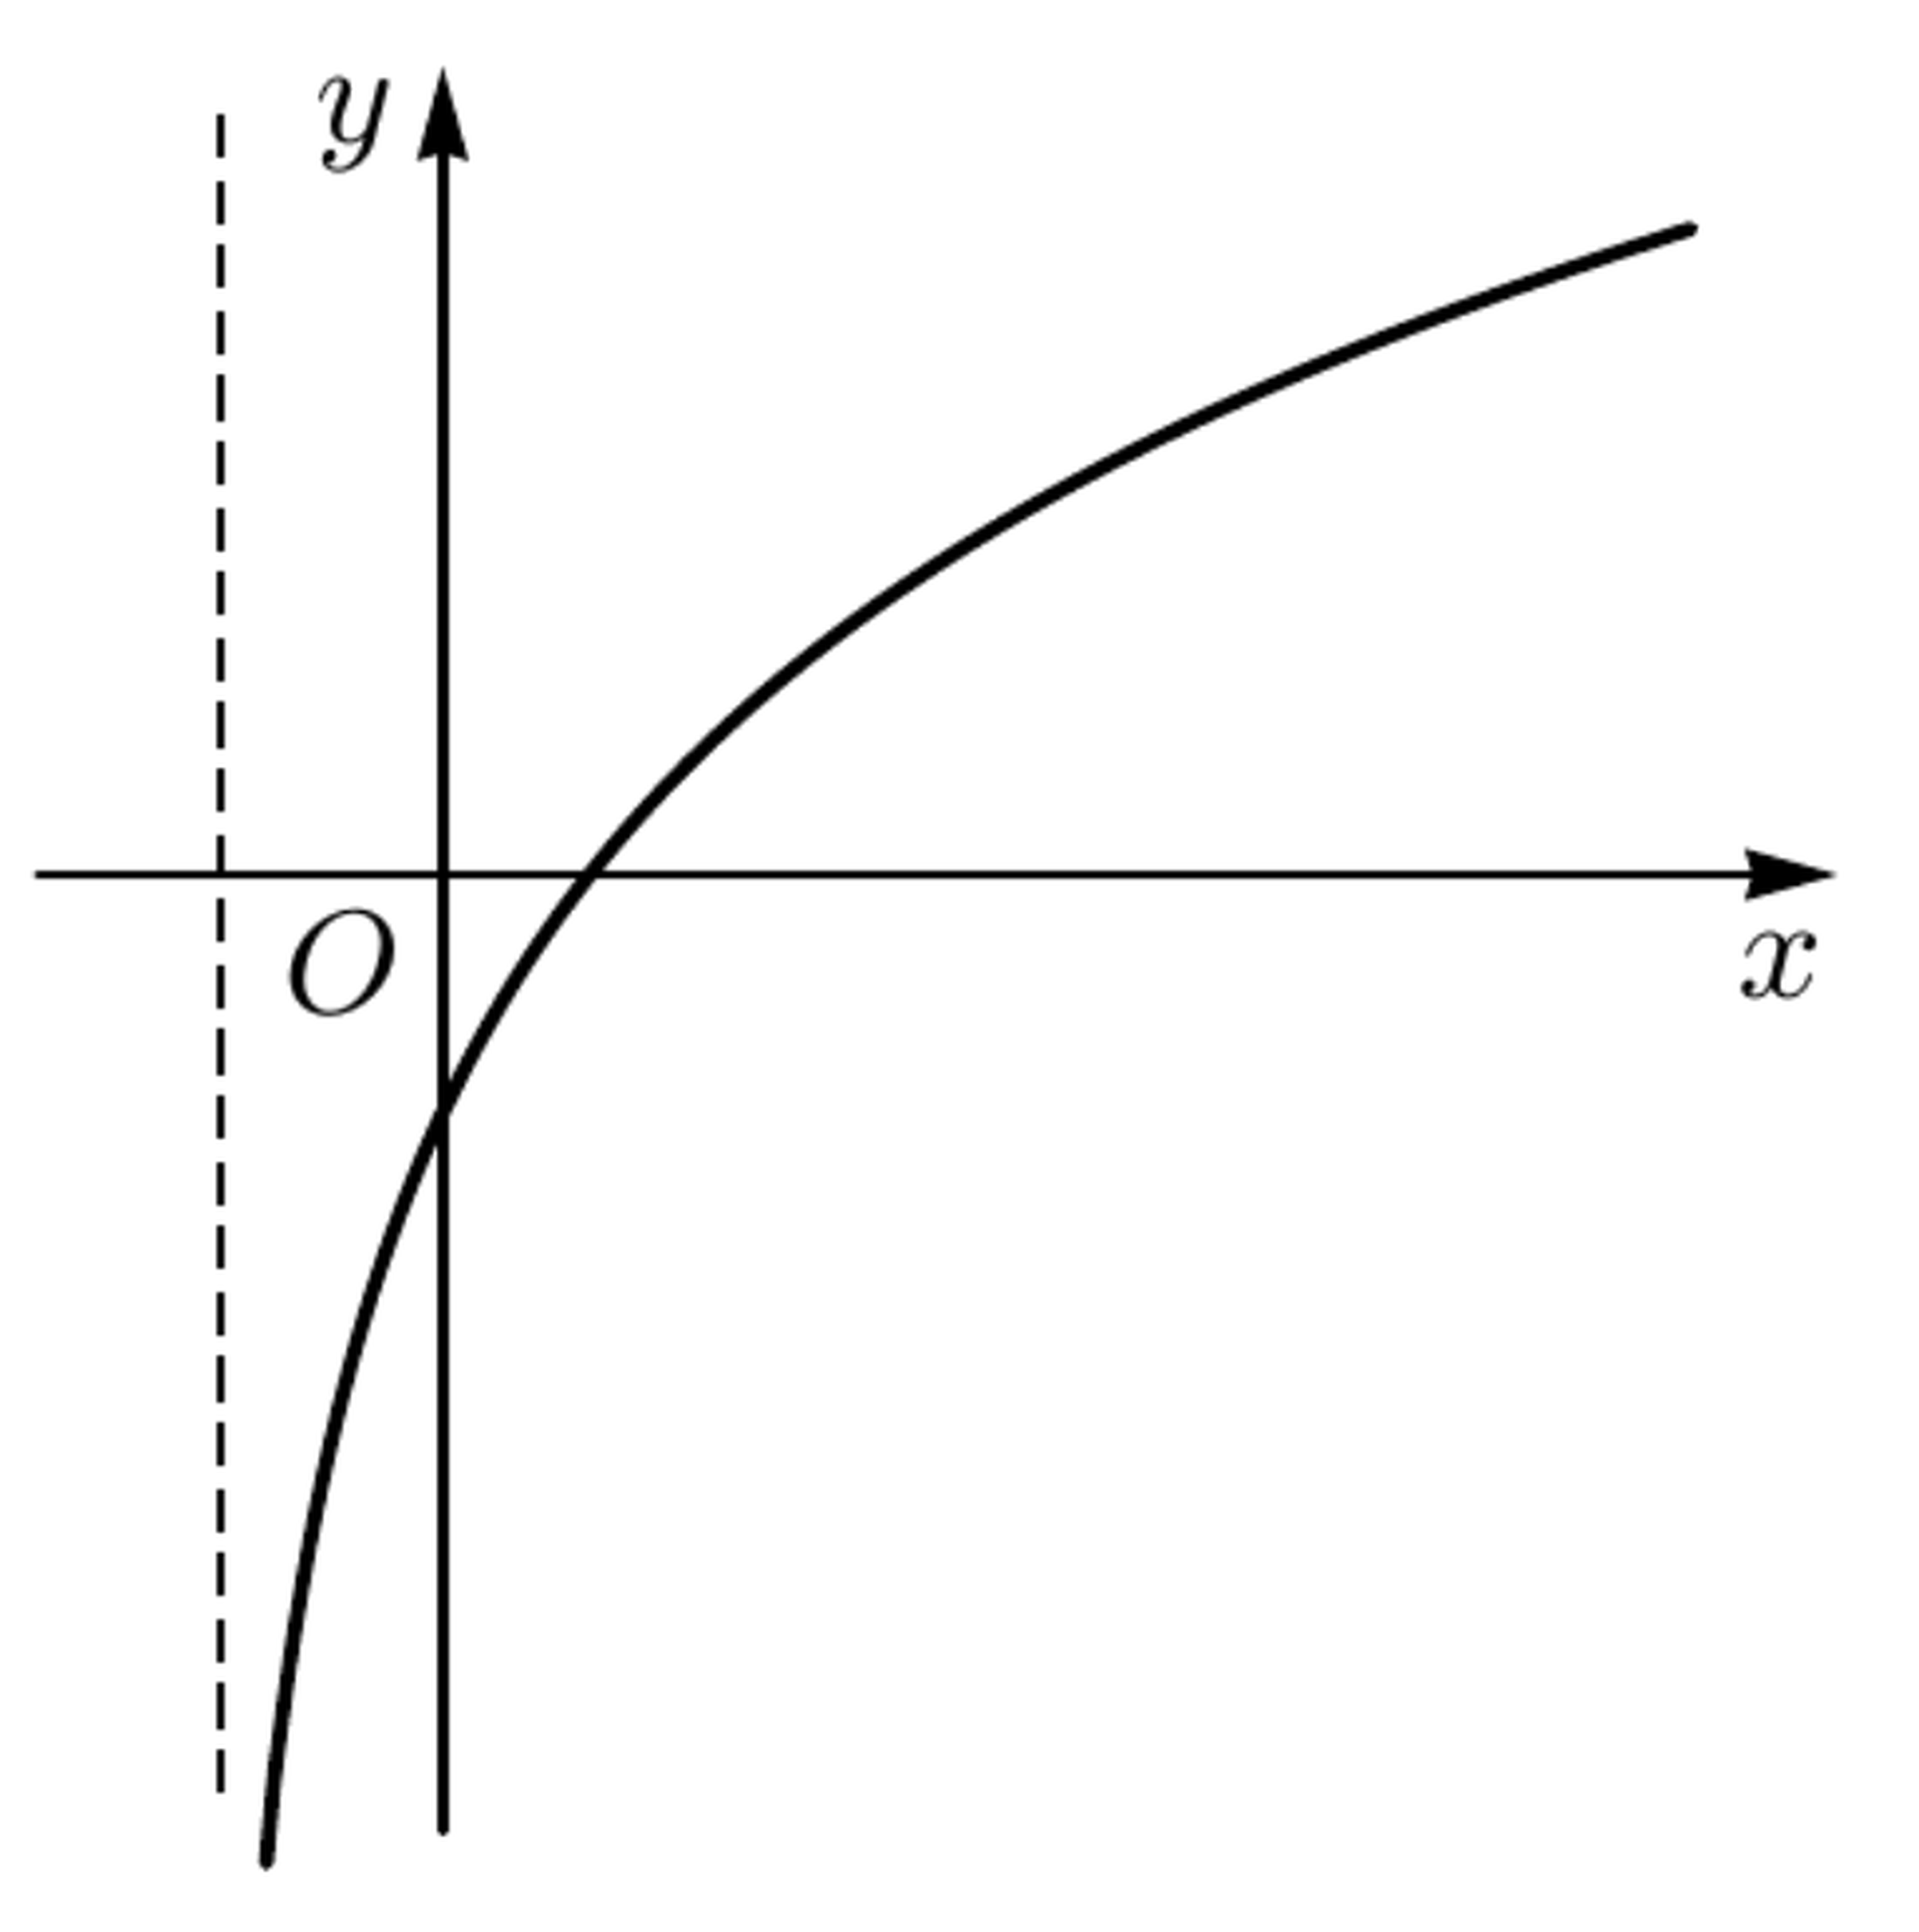
\includegraphics[width=0.42\textwidth]{figures/gao158_q15.png}
\end{center}

\keepwithprev
A. $a>1, b>1$\qquad\qquad B. $a>1, 0<b<1$

C. $0<a<1, b>1$\qquad\qquad D. $0<a<1, 0<b<1$

\ifanswer
\solbegin
\step{图像严格增，得 $a>1$.}
\step{图像与 $y$ 轴交于 $x$ 轴下方，得 $b>0$ 且 $\log_a b<0$，即 $0<b<1$，故选 $B$.}
\solend
\fi

% === Q16 === \lvert\log_2 x\rvert；解析 5 行，故选 C
\item 已知函数 $f(x)=\lvert\log_2 x\rvert$，若 $0<a<b$ 且 $f(a)=f(b)$，则 $a+2b$ 的取值范围是\mbox{（\quad）}

\keepwithprev
A. $(2\sqrt2,+\infty)$\qquad B. $[2\sqrt2,+\infty)$\qquad C. $(3,+\infty)$\qquad D. $[3,+\infty)$

\ifanswer
\solbegin
\step{由 $a<b$ 及 $\lvert\log_2 a\rvert=\lvert\log_2 b\rvert$，得 $\log_2 a=-\log_2 b$，即 $ab=1$，}
\step{且 $0<a<1<b$.}
\step{设 $t=a+2b=2b+\dfrac1b$，则 $t-3=\dfrac{(b-1)(2b-1)}{b}>0$.}
\step{反之，任取 $t>3$，令 $b=\dfrac{t+\sqrt{t^2-8}}{4}>1$、$a=\dfrac1b$，则满足题设且 $a+2b=t$.}
\step{因此取值范围为 $(3,+\infty)$，故选 $C$.}
\solend
\fi

\end{enumerate}

\bigsec{三、解答题}

\begin{enumerate}
\setcounter{enumi}{16}

% === Q17 === 集合、\overline{A}、\subseteq；解析 9 行
\item 已知全集 $U=\R$，集合 $A=\left\{x\mid\dfrac{x-3}{x+1}\leqslant0\right\}$，$B=\{x\mid x^2-2mx+m^2-9<0\}$（$m$ 为实数）.

(1) 当 $m=4$ 时，求 $A\cap B$ 和 $\overline{A}\cup B$；

(2) 若“$x\in A$”是“$x\in B$”的充分条件，求实数 $m$ 的取值范围.

\ifanswer
\solbegin
\step{(1) $\dfrac{x-3}{x+1}\leqslant0\Leftrightarrow-1<x\leqslant3$，所以 $A=(-1,3]$.}
\step{当 $m=4$ 时，$B=\{x\mid(x-4)^2<9\}=(1,7)$，}
\step{于是 $A\cap B=(1,3]$，$\overline{A}\cup B=(-\infty,-1]\cup(1,+\infty)$；}
\step{(2) $x^2-2mx+m^2-9<0\Leftrightarrow(x-m)^2<9$，所以 $B=(m-3,m+3)$.}
\step{题设充分条件等价于 $A\subseteq B$.}
\step{由于 $A=(-1,3]$，左端须满足 $m-3\leqslant-1$.}
\step{又 $3\in A$，须有 $3<m+3$.}
\step{这两个条件也保证 $(-1,3]\subseteq(m-3,m+3)$，}
\step{因此 $A\subseteq B\Leftrightarrow\begin{cases}m-3\leqslant-1\\m+3>3\end{cases}\Leftrightarrow0<m\leqslant2$.}
\solend
\fi

% === Q18 === 蓄水池造价（含 (3) 场地限制）；单位 \mathrm{m}；解析 13 行
\item 某工厂拟建一个容积为 $400\mathrm{m}^3$ 的无盖长方体蓄水池，池深 $4\mathrm{m}$，池底为矩形，其一边长
为 $x\mathrm{m}$. 池壁每平方米造价 100 元，池底每平方米造价 150 元. 设水池的总造价为 $C$
元.

(1) 把 $C$ 表示成 $x$ 的函数，并写出它的定义域；

(2) 当 $x$ 为何值时，总造价最低？最低造价是多少？

(3) 受场地限制，池底一边长 $x$ 不超过 $8\mathrm{m}$，此时总造价最低是多少？

\ifanswer
\solbegin
\step{(1) 设池底另一边长为 $y\mathrm{m}$，则 $4xy=400$，所以 $y=\dfrac{100}{x}$，$x>0$.}
\step{池底面积为 $100\mathrm{m}^2$，池壁总面积为 $8\left(x+\dfrac{100}{x}\right)\mathrm{m}^2$，}
\step{因此 $C(x)=100\times8\left(x+\dfrac{100}{x}\right)+150\times100=800x+\dfrac{80000}{x}+15000$，}
\step{定义域为 $(0,+\infty)$.}
\step{(2) 因为 $x>0$，所以 $C(x)=800\left(x+\dfrac{100}{x}\right)+15000$，}
\step{$\geqslant800\times2\sqrt{x\cdot\dfrac{100}{x}}+15000=31000$，}
\step{当且仅当 $x=\dfrac{100}{x}$，即 $x=10$ 时取等号.}
\step{答：当 $x=10$ 时，总造价最低，为 31000 元.}
\step{(3) 此时定义域为 $(0,8]$. 任取 $0<x_1<x_2\leqslant8$，}
\step{则 $C(x_2)-C(x_1)=800(x_2-x_1)\left(1-\dfrac{100}{x_1x_2}\right)<0$，}
\step{所以 $C(x)$ 在 $(0,8]$ 上严格递减，$x=8$ 时总造价最低，}
\step{且 $C(8)=800\times8+\dfrac{80000}{8}+15000=31400$.}
\step{答：受场地限制时，最低总造价为 31400 元.}
\solend
\fi

% === Q19 === 甲乙滤材 0.8^n／0.7^n；解析 17 行
\item 某环保公司研发了两种新型滤材甲和乙：污水每经过一层甲滤材，污染物含量减少
20\%；每经过一层乙滤材，污染物含量减少 30\%. 每层甲滤材成本 3 万元，每层乙滤材
成本 4 万元. 设原污水中污染物含量为 1，要求处理后污染物含量低于原来的 5\%.

(1) 若只使用一种滤材，污水经过 $n$ 层后污染物含量为 $y$，分别写出使用甲、乙两种滤材
时 $y$ 关于 $n$ 的函数关系式（$n$ 为正整数）；

(2) 若只使用一种滤材，分别求甲、乙至少各需要多少层，并比较哪种滤材的总成本更
低；

(3) 若两种滤材可以混合使用（先后顺序不影响效果），设使用甲滤材 $m$ 层、乙滤材 $n$
层（$m$、$n$ 为非负整数），求满足要求的最低总成本，并指出此时 $m$、$n$ 的值.

\ifanswer
\solbegin
\step{(1) 甲：$y=0.8^n$；乙：$y=0.7^n$，其中 $n$ 为正整数.}
\step{(2) 两种滤材均须满足 $y<0.05$，且污染物含量随层数增加而严格减少.}
\step{$0.8^{14}\approx0.04398<0.05<0.05498\approx0.8^{13}$，}
\step{$0.7^9=0.040353607<0.05<0.05764801=0.7^8$，}
\step{甲至少需要 14 层，成本为 $3\times14=42$ 万元；}
\step{乙至少需要 9 层，成本为 $4\times9=36$ 万元.}
\step{因此，只使用一种滤材时，使用乙滤材的总成本更低.}
\step{(3) 设总成本为 $C$ 万元，则 $C=3m+4n,0.8^m\cdot0.7^n<0.05,m,n\in\{0,1,2,\cdots\}$，}
\step{若 $m\geqslant3$，将其中 3 层甲替换为 2 层乙，}
\step{因为 $0.7^2=0.49<0.512=0.8^3,2\times4<3\times3$，}
\step{替换后污染物含量更低，成本减少 1 万元，因此最低成本方案必有 $m\leqslant2$.}
\step{当 $m=0$ 时，由第（2）小题得至少需要 9 层乙，最低成本为 36 万元.}
\step{当 $m=1$ 或 $m=2$ 时，$0.8\cdot0.7^7>0.8^2\cdot0.7^7=0.052706752>0.05$，}
\step{$0.8^2\cdot0.7^8<0.8\cdot0.7^8=0.046118408<0.05$，}
\step{因此两种情形均至少需要 8 层乙，}
\step{对应最低成本分别为 $3+4\times8=35$ 万元，$3\times2+4\times8=38$ 万元.}
\step{答：满足要求的最低总成本为 35 万元，此时使用甲滤材 1 层、乙滤材 8 层.}
\solend
\fi

% === Q20 === f(x)=\log_2(4^x+1)-x；\Delta；解析 17 行
\item 已知函数 $f(x)=\log_2(4^x+1)-x$.

(1) 证明 $f(x)=\log_2(2^x+2^{-x})$，并求 $f(x)$ 的最小值及取得最小值时 $x$ 的值；

(2) 解不等式 $f(x)>\log_2 5-1$；

(3) 证明：函数 $f(x)$ 在区间 $[0,+\infty)$ 上是严格增函数；并求使关于 $x$ 的方程 $f(x)=m$ 恰
有两个不同实数解的实数 $m$ 的取值范围.

\ifanswer
\solbegin
\step{(1) $f(x)=\log_2(4^x+1)-\log_2 2^x=\log_2\dfrac{4^x+1}{2^x}=\log_2(2^x+2^{-x})$，}
\step{因为 $2^x+2^{-x}\geqslant2\sqrt{2^x\cdot2^{-x}}=2$，所以 $f(x)\geqslant\log_2 2=1$，}
\step{等号当且仅当 $2^x=2^{-x}$，即 $x=0$ 时成立，故最小值为 1.}
\step{(2) 令 $t=2^x>0$，则 $f(x)>\log_2 5-1\Leftrightarrow t+\dfrac1t>\dfrac52\Leftrightarrow2t^2-5t+2>0$}
\step{$\Leftrightarrow(2t-1)(t-2)>0$，}
\step{结合 $t>0$，得 $0<t<\dfrac12$ 或 $t>2$，即 $x<-1$ 或 $x>1$，}
\step{解集为 $(-\infty,-1)\cup(1,+\infty)$.}
\step{(3) 任取 $0\leqslant x_1<x_2$，记 $a=2^{x_1}$，$b=2^{x_2}$，则 $1\leqslant a<b$，$ab>1$，}
\step{从而 $\left(b+\dfrac1b\right)-\left(a+\dfrac1a\right)=(b-a)\left(1-\dfrac{1}{ab}\right)>0$，}
\step{由对数函数的严格递增性，得 $f(x_1)<f(x_2)$，}
\step{所以 $f(x)$ 在 $[0,+\infty)$ 上是严格增函数.}
\step{当 $m<1$ 时，由（1）得方程无实数解；当 $m=1$ 时，只有实数解 $x=0$.}
\step{当 $m>1$ 时，令 $t=2^x>0$，则 $f(x)=m\Leftrightarrow t+\dfrac1t=2^m\Leftrightarrow t^2-2^m t+1=0$，}
\step{此时 $\Delta=2^{2m}-4>0$，两根之和为 $2^m>0$、之积为 $1>0$，}
\step{故有两个不同的正根.}
\step{每个正根 $t$ 唯一确定一个实数 $x=\log_2 t$，故原方程恰有两个不同实数解，}
\step{所求范围为 $m\in(1,+\infty)$.}
\solend
\fi

% === Q21 === f(x)=4^x-m\cdot2^{x+1}+3 值域与 h(m) 分段；解析 13 行
\item 已知函数 $f(x)=4^x-m\cdot2^{x+1}+3$（$m\in\R$），$x\in[0,2]$.

(1) 当 $m=1$ 时，求 $f(x)$ 的值域；

(2) 记 $f(x)$ 的最小值为 $h(m)$，求 $h(m)$ 的表达式；

(3) 若关于 $x$ 的方程 $f(x)=0$ 在区间 $[0,2]$ 上有解，求实数 $m$ 的取值范围.

\ifanswer
\solbegin
\step{令 $t=2^x$，则 $t\in[1,4]$，且 $f(x)=t^2-2mt+3=(t-m)^2+3-m^2$，}
\step{(1) 当 $m=1$ 时，$f(x)=(t-1)^2+2$.}
\step{由 $0\leqslant t-1\leqslant3$，得 $2\leqslant f(x)\leqslant11$，值域为 $[2,11]$.}
\step{(2) 二次函数 $y=(t-m)^2+3-m^2$ 的对称轴为直线 $t=m$.}
\step{当 $m\leqslant1$ 时，在 $t=1$ 处取最小值；}
\step{当 $1<m<4$ 时，在 $t=m$ 处取最小值；}
\step{当 $m\geqslant4$ 时，在 $t=4$ 处取最小值；}
\step{因此 $h(m)=\begin{cases}4-2m,&m\leqslant1\\3-m^2,&1<m<4\\19-8m,&m\geqslant4\end{cases}$；}
\step{(3) 方程 $f(x)=0$ 在 $[0,2]$ 上有解，}
\step{等价于存在 $t\in[1,4]$，使 $m=\dfrac{t^2+3}{2t}=\dfrac12\left(t+\dfrac3t\right)$，}
\step{由基本不等式，$m\geqslant\dfrac12\cdot2\sqrt{t\cdot\dfrac3t}=\sqrt3$，当且仅当 $t=\sqrt3$ 时取等号；}
\step{又 $\dfrac{19}{8}-m=\dfrac{(4-t)(4t-3)}{8t}\geqslant0$，当且仅当 $t=4$ 时取等号；}
\step{因此必有 $\sqrt3\leqslant m\leqslant\dfrac{19}{8}$.}
\solend
\fi

\end{enumerate}

\end{document}
"
% 紧凑版：xelatex "\def\iscompact{1}% 高一158_上实东滩_期中.tex
%   —— 高一上数学"2026-2027 年上实东滩高一上期中"（试卷版/答案版/紧凑版）
% 试卷版：xelatex 高一158_上实东滩_期中.tex
% 答案版：xelatex "\def\isanswer{1}\input{高一158_上实东滩_期中.tex}"
% 紧凑版：xelatex "\def\iscompact{1}\input{高一158_上实东滩_期中.tex}"
%
% ① 原始材料：微信公众号"魔都数学加油站"文章，连载"27学年高一158"，原文标题
% "27学年高一158——2026-2027年上海市上实东滩高一上期中"（本卷本地编号 158 与
% 原卷连载号一致，无撞号）。
% 正文为 9 张 PNG 页（01/05/08/09 为 2560×3620，02/03/04/06/07 为 4762×6735，
% 同一篇各页分辨率混排，逐页按各自分辨率裁图核对）。
% 体例：讲评版——填空 3—12（10 题）、选择 13—16（4 题）、解答 17—21（5 题），
% 共 19 题，自第 3 题起编（1、2 未印在本篇）；Q5 只印【答案】、其余 18 题
% 逐题印【解析】（逐题核实，见 ②）。题目、答案、解析均据原图转录；卷面粉红色
% 水印"魔都数学加油站"及公众号页脚未录入。全卷末题为第 21 题，无附加题节。
% 全卷 2 组配图（逐页通读 9 页确认）——
%   · Q10 题干右侧"曼 → man"字形变换图（02 页），题目配图、三版都出，
%     裁 figures/gao158_q10.png；
%   · Q15 题干"如图所示"对数函数大致图像（03 页右下），题目配图、三版都出，
%     裁 figures/gao158_q15.png；
% 2 图均取自原卷截图，去粉色水印、转灰度、4× LANCZOS 放大；
% 其余各页逐页确认无其它题目配图、无解析内配图、无表格。
%
% 卷首标题：原卷印作"2026-2027 年上实东滩高一上期中"，年份区间按全稿惯例排 en dash；
% 原卷卷面未印副标题，本稿按同期中卷知识模块口径补出"集合与常用逻辑用语、不等式、函数"。
%
% ② 与原卷的排版差异／照录项清单：
%   ① 原文从第 3 题起，本稿保留原题号；共 19 题三节，解答题 5 题到 21；
%      三节各自一个 enumerate＋各自 \setcounter{enumi}{2}／{12}／{16}，
%      不贯穿（题目溯源.py 按 \bigsec 切节、每节独立计 depth，只收 depth==1 的 \item）；
%   ② 混合体例：Q5 只印【答案】、无【解析】，按 高一156 第 3 题成例另提
%      \ans{}、不补造解析；其余 18 题印【解析】、用 \solbegin…\solend；
%      四道选择题答案均在解析末句"故选 C／B／B／C"（逐个放大复核）、
%      题干括号 \mbox{（\quad）} 留空、不另提 \ans{}；答案版
%      【答案】/【解析】标记数 = 19 = 全卷题数（1 个 \ans ＋ 18 个 \solbegin）；
%   ③ 原卷卷面未印副标题，本稿按知识模块口径补出；
%   ④ 原卷填空横线按全稿惯例排 \blankline[4.4em]；选择题选项段前按惯例各加
%      \keepwithprev；解答题不留作答区、不加 \anspace（原卷为讲评版）；
%   ⑤ 数集：Q13"在 \R 上严格递增"、Q14"$x\in\R$"、Q17"$U=\R$"、
%      Q21"$m\in\R$" 原卷印正体粗体 R，按全稿惯例归一 \R；
%      绝对值排 \lvert…\rvert（Q12 $\lvert a\rvert$、Q14 $\lvert x-2\rvert$、
%      Q16 $\lvert\log_2 x\rvert$／$\lvert\log_2 a\rvert$／$\lvert\log_2 b\rvert$），
%      集合描述竖线排 \mid（Q17），不等号按全稿惯例排 \leqslant／\geqslant，
%      补集上划线 \overline{A}（Q17）；
%   ⑥ 子集／真子集符号逐处照录不统一：Q14 解析"$(2,3)\subsetneq(1,3)$"原卷印
%      带下划线且被斜杠划过的 ⊊（真子集，放大 03 页确认），照录 \subsetneq；
%      Q17 解析三处"$A\subseteq B$""$(-1,3]\subseteq(m-3,m+3)$"原卷印
%      带下划线 ⊆（放大 05 页确认），照录 \subseteq；本卷无单线 \subset 用例；
%   ⑦ 判别式：Q20 (3) 解析"$\Delta=2^{2m}-4>0$"原卷印高瘦等腰 \Delta
%      （像素实测高/宽 ≈ 1.13，扁三角 \triangle 为 0.93，放大 08 页确认），
%      照录 \Delta；本卷无扁三角 \triangle 用例；
%   ⑧ "图像"与"图象"：全卷统一用"图像"（Q6 题干、Q10 两处、Q11 解析、
%      Q15 题干与解析两处，逐处放大确认带单人旁），照录不改；
%   ⑨ 中文弯引号照录：Q5 命题"若实数…"、Q10"曼""man""新"、Q14 题干与
%      解析的两则不等式、Q17 (2)"$x\in A$""$x\in B$"；注释里一律 ASCII 引号；
%   ⑩ 半角逗号逐处照录：Q8"$2,3,4$""$-2,-1,0$"、Q10 点坐标 $(x,y)$／
%      $(t,2^t-1)$／$(1-2^t,t)$、Q15 四选项"$a>1, b>1$"等、
%      Q19 (3)"$C=3m+4n,0.8^m\cdot0.7^n<0.05,m,n\in\{0,1,2,\cdots\}$"
%      与"$0.7^2=0.49<0.512=0.8^3,2\times4<3\times3$"、
%      Q21 cases 内"$4-2m,$"等；其余行中逗号／顿号照录全角；
%      行末西文句点 ASCII `.`；
%   ⑪ 顿号照录：Q3"（用 $a$、$b$ 表示）"、Q5"$x$、$y$"、Q13"A、B"、
%      Q16 解析"$>1$、$a=\dfrac1b$"、Q19"甲、乙""$m$、$n$"、
%      Q20"$2^m>0$、之积为"、Q21"$m$、$n$"；顿号一律移到数学模式外，
%      数学模式内不出现中文标点；
%   ⑫ 角度与单位照录：Q10 三处"$90^{\circ}$"、Q18"$400\mathrm{m}^3$"
%      "$4\mathrm{m}$""$x\mathrm{m}$""$8\mathrm{m}$""$y\mathrm{m}$"
%      "$100\mathrm{m}^2$""$\left(x+\dfrac{100}{x}\right)\mathrm{m}^2$"；
%      Q19 百分号"20\%""30\%""5\%"按原卷排 \%；
%   ⑬ 文本模式全角括号照录：Q10"（提示：…）"、Q17"（$m$ 为实数）"、
%      Q19"（$n$ 为正整数）""（先后顺序不影响效果）""（$m$、$n$ 为非负整数）"、
%      Q20"由（1）得"、Q19"由第（2）小题"、Q21"（$m\in\R$）"；
%      子题行首标号按全稿惯例用半角 (1)(2)(3)；
%   ⑭ 复杂式照录别简化：Q3 $\dfrac{\log_3 2+\log_3 5}{\log_3 3+2\log_3 2}$、
%      Q8 $[-3,-2)\cup(4,5]$、Q9 $18ab=2^t\cdot3^t=6^t=a+b$、
%      Q12 $\dfrac{\sqrt6}{2}$、Q18 $C(8)=800\times8+\dfrac{80000}{8}+15000=31400$
%      （原卷即 C(8)，非 C(2)）、Q19 $0.8^{14}\approx0.04398$、
%      $0.7^9=0.040353607$、$0.052706752$、$0.046118408$、
%      Q20 $t^2-2^m t+1=0$、Q21 $h(m)$ 三段 cases 与 $\dfrac{(4-t)(4t-3)}{8t}$ 等；
%      \left…\right 不得拆到不同 $…$ 组；cases 块整体算一个印刷行；
%   ⑮ 一条 \step = 原卷解析的一个印刷行；别并折行、别拆行。跨页续印按题合并
%      （Q7 的 01—02 页、Q9/Q10/Q11 的 02—03 页、Q13/Q14 的 03 页上下、
%      Q15/Q16 的 04 页上下、Q17 的 04—05 页、Q18 的 05—06 页、
%      Q19 的 06—07 页、Q20 的 07—08 页、Q21 的 08—09 页）；
%      跨半页重叠行（Q5【答案】、Q9 设公共值行、Q10 题干、Q16 反之行、
%      Q18 (2) 题干、Q19 末两行、Q20 (3) 末行、Q21 cases 块）只算一个印刷行；
%   ⑯ 配图：2 组题目配图（见 ①），均三版都出，\needvspace 守卫放 \item 之前
%      把"题干＋图"整块推走，\includegraphics 放题干之后；本卷无解析内配图、
%      无红字加粗小标题（全卷逐页确认，故无 \stepm）。
%
% ③ 行数复核：一条 \step = 原卷解析的一个印刷行，cases 块作一个印刷行计。
%   逐题数（逐页核对）：Q3：1；Q4：2；Q5：0（只印【答案】、提 \ans{}，
%   不计入 \step 账）；Q6：1；Q7：4；Q8：5；Q9：2；Q10：2；Q11：3；
%   Q12：3；Q13：2；Q14：3；Q15：2；Q16：5；Q17：9；Q18：13；
%   Q19：17；Q20：17；Q21：13。
%   合计 104 行（104 条 \step ＋ 0 条 \stepm），与原卷逐题印刷行相等。
%   全卷 19 题：Q5 一处 \ans{} ＋ 其余 18 题设 \solbegin…\solend，
%   答案版【答案】/【解析】标记数 = 19 = 全卷题数。
%
% ④ 页码分布（供回原图复核）：
%   卷首标题＋"一、填空题"＋Q3 题干＋解析 1 行、Q4 题干＋解析 2 行、
%   Q5 题干＋【答案】在 01 页上半；Q5【答案】（重叠重印）＋Q6 题干＋解析 1 行、
%   Q7 题干＋解析前 3 行在 01 页下半；Q7 解析末行＋Q8 题干＋解析 5 行、
%   Q9 题干＋解析首行在 02 页上半；Q9 解析末行＋Q10 题干（含"曼→man"图）
%   ＋解析 2 行＋Q11 题干＋解析首行在 02 页下半；Q11 解析后 2 行＋Q12 题干
%   ＋解析 3 行＋"二、选择题"标题＋Q13 题干＋选项在 03 页上半；
%   Q13 选项（重叠重印）＋解析 2 行＋Q14 题干＋选项＋解析 3 行＋Q15 题干
%   ＋对数图像（右侧）在 03 页下半；Q15 选项＋解析 2 行＋Q16 题干＋选项
%   ＋解析前 4 行在 04 页上半；Q16 解析末行＋"三、解答题"标题＋Q17 题干
%   ＋两问＋解析 (1) 3 行在 04 页下半；Q17 解析 (2) 6 行＋Q18 题干＋三问
%   ＋解析 (1) 4 行＋(2) 首行在 05 页上下；Q18 解析 (2) 后 3 行＋(3) 5 行
%   ＋Q19 题干＋三问＋解析 (1) 1 行＋(2) 3 行在 06 页上下；Q19 解析 (2) 3 行
%   ＋(3) 12 行在 07 页上半；Q19 解析末 2 行（重叠）＋Q20 题干＋三问
%   ＋解析 (1) 3 行在 07 页下半；Q20 解析 (2) 4 行＋(3) 前 4 行在 08 页上半；
%   Q20 解析 (3) 后 6 行＋Q21 题干＋(1) 问在 08 页下半；Q21 (2)(3) 问＋
%   解析 (1) 3 行＋(2) 5 行＋cases 块在 09 页上半；Q21 cases 块（重叠）
%   ＋(3) 解析 5 行在 09 页下半。本稿按题连排，不丢行、不并折行；
%   全卷末题为第 21 题，无附加题节。
%
% ⑤ 存疑／需主会话回原图复核：
%   1. Q14 解析"$(2,3)\subsetneq(1,3)$"的 ⊊（真子集带斜杠）与 Q17 的 ⊆
%      是两种不同记号，本稿分别照录 \subsetneq／\subseteq，请复核；
%   2. Q20 (3)"$\Delta=2^{2m}-4>0$"判为高瘦 \Delta，请复核是否 \triangle；
%   3. 任务书提示"Q18 解析里印 C(2)=…"，但 06 页原图逐处读作
%      $C(8)=800\times8+\dfrac{80000}{8}+15000=31400$，未找到 C(2)，
%      本稿照原卷排 C(8)，请复核；
%   4. Q19 解析末句"最低总成本为 35 万元"（07 页上下两处印同），
%      OCR 曾误读为 34，本稿按 35 照录，请复核；
%   5. Q10 提示末尾"坐标为 $(-y,x)$）."为半角 $)$＋全角 $）$ 两枚括号，
%      本稿照录，请复核；
%   6. Q21 cases 块后"；"落在分式中行右侧（排版居中基线所致），
%      本稿排作 $…\end{cases}$；，请复核。
%   全卷除此 6 类外未发现其它笔误／自相矛盾处；19 题中 18 题印【解析】。
%
\documentclass[a4paper,11pt]{article}
\usepackage{common}

\begin{document}

\examtitlest[3]{2026--2027 年上实东滩高一上期中}{集合与常用逻辑用语、不等式、函数}

\bigsec{一、填空题}

\begin{enumerate}
\setcounter{enumi}{2}

% === Q3 === 换底公式；解析 1 行
\item 已知 $3^a=5$，$\log_3 2=b$，则 $\log_{12} 10=$\blankline[4.4em]（用 $a$、$b$ 表示）.

\ifanswer
\solbegin
\step{$\log_{12} 10=\dfrac{\log_3 2+\log_3 5}{\log_3 3+2\log_3 2}=\dfrac{a+b}{1+2b}$.}
\solend
\fi

% === Q4 === 定义域；解析 2 行；半角括号 ( ) 与全角逗号照录
\item 函数 $y=\sqrt{2-x}+\lg(x^2-1)$ 的定义域为\blankline[4.4em].

\ifanswer
\solbegin
\step{由 $2-x\geqslant0$ 且 $x^2-1>0$，得 $x\leqslant2$ 且 ($x<-1$或$x>1$)，}
\step{定义域为 $(-\infty,-1)\cup(1,2]$.}
\solend
\fi

% === Q5 === 只印【答案】、无【解析】；反证法，中文弯引号
\item 用反证法证明命题“若实数 $x$、$y$ 满足 $x+y>2$，则 $x$、$y$ 中至少有一个大于 1”时，
应假设\blankline[4.4em].

\ifanswer
\ans{$x\leqslant1$ 且 $y\leqslant1$}
\fi

% === Q6 === 图像平移；解析 1 行
\item 函数 $y=\dfrac{2x+1}{x-1}$ 的图像可由函数 $y=\dfrac{3}{x}$ 的图像先向右平移 $a$ 个单位，再向上平移 $b$ 个单位
得到，则 $a+b=$\blankline[4.4em].

\ifanswer
\solbegin
\step{$y=\dfrac{2x+1}{x-1}=\dfrac{3}{x-1}+2$，所以 $a=1$，$b=2$，$a+b=3$.}
\solend
\fi

% === Q7 === 集合三元子集；解析 4 行，跨 01—02 页
\item 设 $A=\{a_1,a_2,a_3,a_4\}$ 是由四个实数组成的集合，若 $A$ 的所有三元子集中，三个元素之和
组成的集合为 $B=\{1,4,7,12\}$，则集合 $A=$\blankline[4.4em].

\ifanswer
\solbegin
\step{设 $S=a_1+a_2+a_3+a_4$，}
\step{每个元素在四个三元子集中恰出现三次，则 $3S=1+4+7+12=24$，得 $S=8$.}
\step{四个三元子集的元素和分别为 $S-a_i$，}
\step{所以 $A=\{8-1,8-4,8-7,8-12\}=\{-4,1,4,7\}$.}
\solend
\fi

% === Q8 === 不等式整数解；解析 5 行；半角逗号照录
\item 不等式 $x^2-(a+1)x+a<0$ 的解集中恰有 3 个整数，则 $a$ 的取值范围是\blankline[4.4em].

\ifanswer
\solbegin
\step{原不等式为 $(x-1)(x-a)<0$；}
\step{$a=1$ 时解集为空集，不符合题意.}
\step{若 $a>1$，解集为 $(1,a)$，恰含整数 $2,3,4$，则 $4<a\leqslant5$.}
\step{若 $a<1$，解集为 $(a,1)$，恰含整数 $-2,-1,0$，则 $-3\leqslant a<-2$.}
\step{故 $a$ 的取值范围是 $[-3,-2)\cup(4,5]$.}
\solend
\fi

% === Q9 === 对数换底＋指数；解析 2 行
\item 已知正数 $a$、$b$ 满足 $1+\log_2 a=2+\log_3 b=\log_6(a+b)$，则 $\dfrac1a+\dfrac1b=$\blankline[4.4em].

\ifanswer
\solbegin
\step{设公共值为 $t$，则 $2a=2^t$，$9b=3^t$，$a+b=6^t$，}
\step{于是 $18ab=2^t\cdot3^t=6^t=a+b$，即 $\dfrac1a+\dfrac1b=\dfrac{a+b}{ab}=18$.}
\solend
\fi

% === Q10 === "曼"字旋转 90°；题目配图（三版都出）；解析 2 行
\needvspace{6cm}
\item 网上流传一个有趣的字形变换：把汉字“曼”的右半部分旋转 $90^{\circ}$，就得到英文单词
“man”的艺术字. 数学中，把曲线绕原点旋转也会得到“新”的曲线：将函数
$y=2^x-1$ 的图像绕坐标原点 $O$ 逆时针旋转 $90^{\circ}$，得到的曲线恰是某个函数的
图像，则这个函数的解析式为\blankline[4.4em]（提示：点 $(x,y)$ 绕 $O$ 逆时针旋转 $90^{\circ}$ 后的
坐标为 $(-y,x)$）.

\begin{center}

\includegraphics[width=0.42\textwidth]{figures/gao158_q10.png}
\end{center}

\ifanswer
\solbegin
\step{原图像上的点 $(t,2^t-1)$ 旋转后为 $(1-2^t,t)$.}
\step{记其为 $(x,y)$，则 $x=1-2^y$，即 $y=\log_2(1-x)$，定义域为 $(-\infty,1)$.}
\solend
\fi

% === Q11 === 值域；解析 3 行，跨 02—03 页
\item 函数 $f(x)=\sqrt{x-2}-\sqrt{15-3x}$ 的值域为\blankline[4.4em].

\ifanswer
\solbegin
\step{由 $x-2\geqslant0$ 且 $15-3x\geqslant0$，得定义域为 $[2,5]$.}
\step{在 $[2,5]$ 上，$\sqrt{x-2}$ 与 $-\sqrt{15-3x}$ 均严格递增，因此 $f(x)$ 严格递增.}
\step{$f(2)=-3$，$f(5)=\sqrt3$，结合函数的图像，值域为 $[-3,\sqrt3]$.}
\solend
\fi

% === Q12 === 绝对值 \lvert…\rvert；解析 3 行
\item 设实数 $a$ 满足 $a<4a^3-5a<\lvert a\rvert$，则 $a$ 的取值范围是\blankline[4.4em].

\ifanswer
\solbegin
\step{由 $a<\lvert a\rvert$ 得 $a<0$，原不等式为 $a<4a^3-5a<-a$.}
\step{同除以 $a<0$，得 $1>4a^2-5>-1\Leftrightarrow1<a^2<\dfrac32$，结合 $a<0$，}
\step{得 $-\dfrac{\sqrt6}{2}<a<-1$，故解集为 $\left(-\dfrac{\sqrt6}{2},-1\right)$.}
\solend
\fi

\end{enumerate}

\bigsec{二、选择题}

\begin{enumerate}
\setcounter{enumi}{12}

% === Q13 === \R 归一；解析 2 行，故选 C
\item 已知 $a>b$，则下列不等式一定成立的是\mbox{（\quad）}

\keepwithprev
A. $\dfrac1a<\dfrac1b$\qquad B. $a^2>b^2$\qquad C. $a^3>b^3$\qquad D. $ac^2>bc^2$

\ifanswer
\solbegin
\step{幂函数 $y=x^3$ 在 $\R$ 上严格递增，$a>b\Rightarrow a^3>b^3$，C 正确.}
\step{取 $a=1$，$b=-1$ 得 A、B 不成立；取 $c=0$ 得 D 不成立；故选 $C$.}
\solend
\fi

% === Q14 === \subsetneq 真子集；解析 3 行，故选 B
\item 设 $x\in\R$，则“$\lvert x-2\rvert<1$”是“$x^2-5x+6<0$”的\mbox{（\quad）}

\keepwithprev
A. 充分非必要条件\qquad\qquad B. 必要非充分条件

C. 充要条件\qquad\qquad D. 既非充分又非必要条件

\ifanswer
\solbegin
\step{$\lvert x-2\rvert<1\Leftrightarrow1<x<3$，$x^2-5x+6<0\Leftrightarrow(x-2)(x-3)<0\Leftrightarrow2<x<3$.}
\step{由 $(2,3)\subsetneq(1,3)$，得“$\lvert x-2\rvert<1$”是“$x^2-5x+6<0$”的必要非充分条件，}
\step{故选 $B$.}
\solend
\fi

% === Q15 === 对数函数大致图像（题目配图，三版都出）；解析 2 行，故选 B
\needvspace{9cm}
\item 已知函数 $f(x)=\log_a(x+b)$（$a>0$ 且 $a\ne1$）的大致图像如图所示，则 $a$、$b$ 满足
的关系是\mbox{（\quad）}

\begin{center}
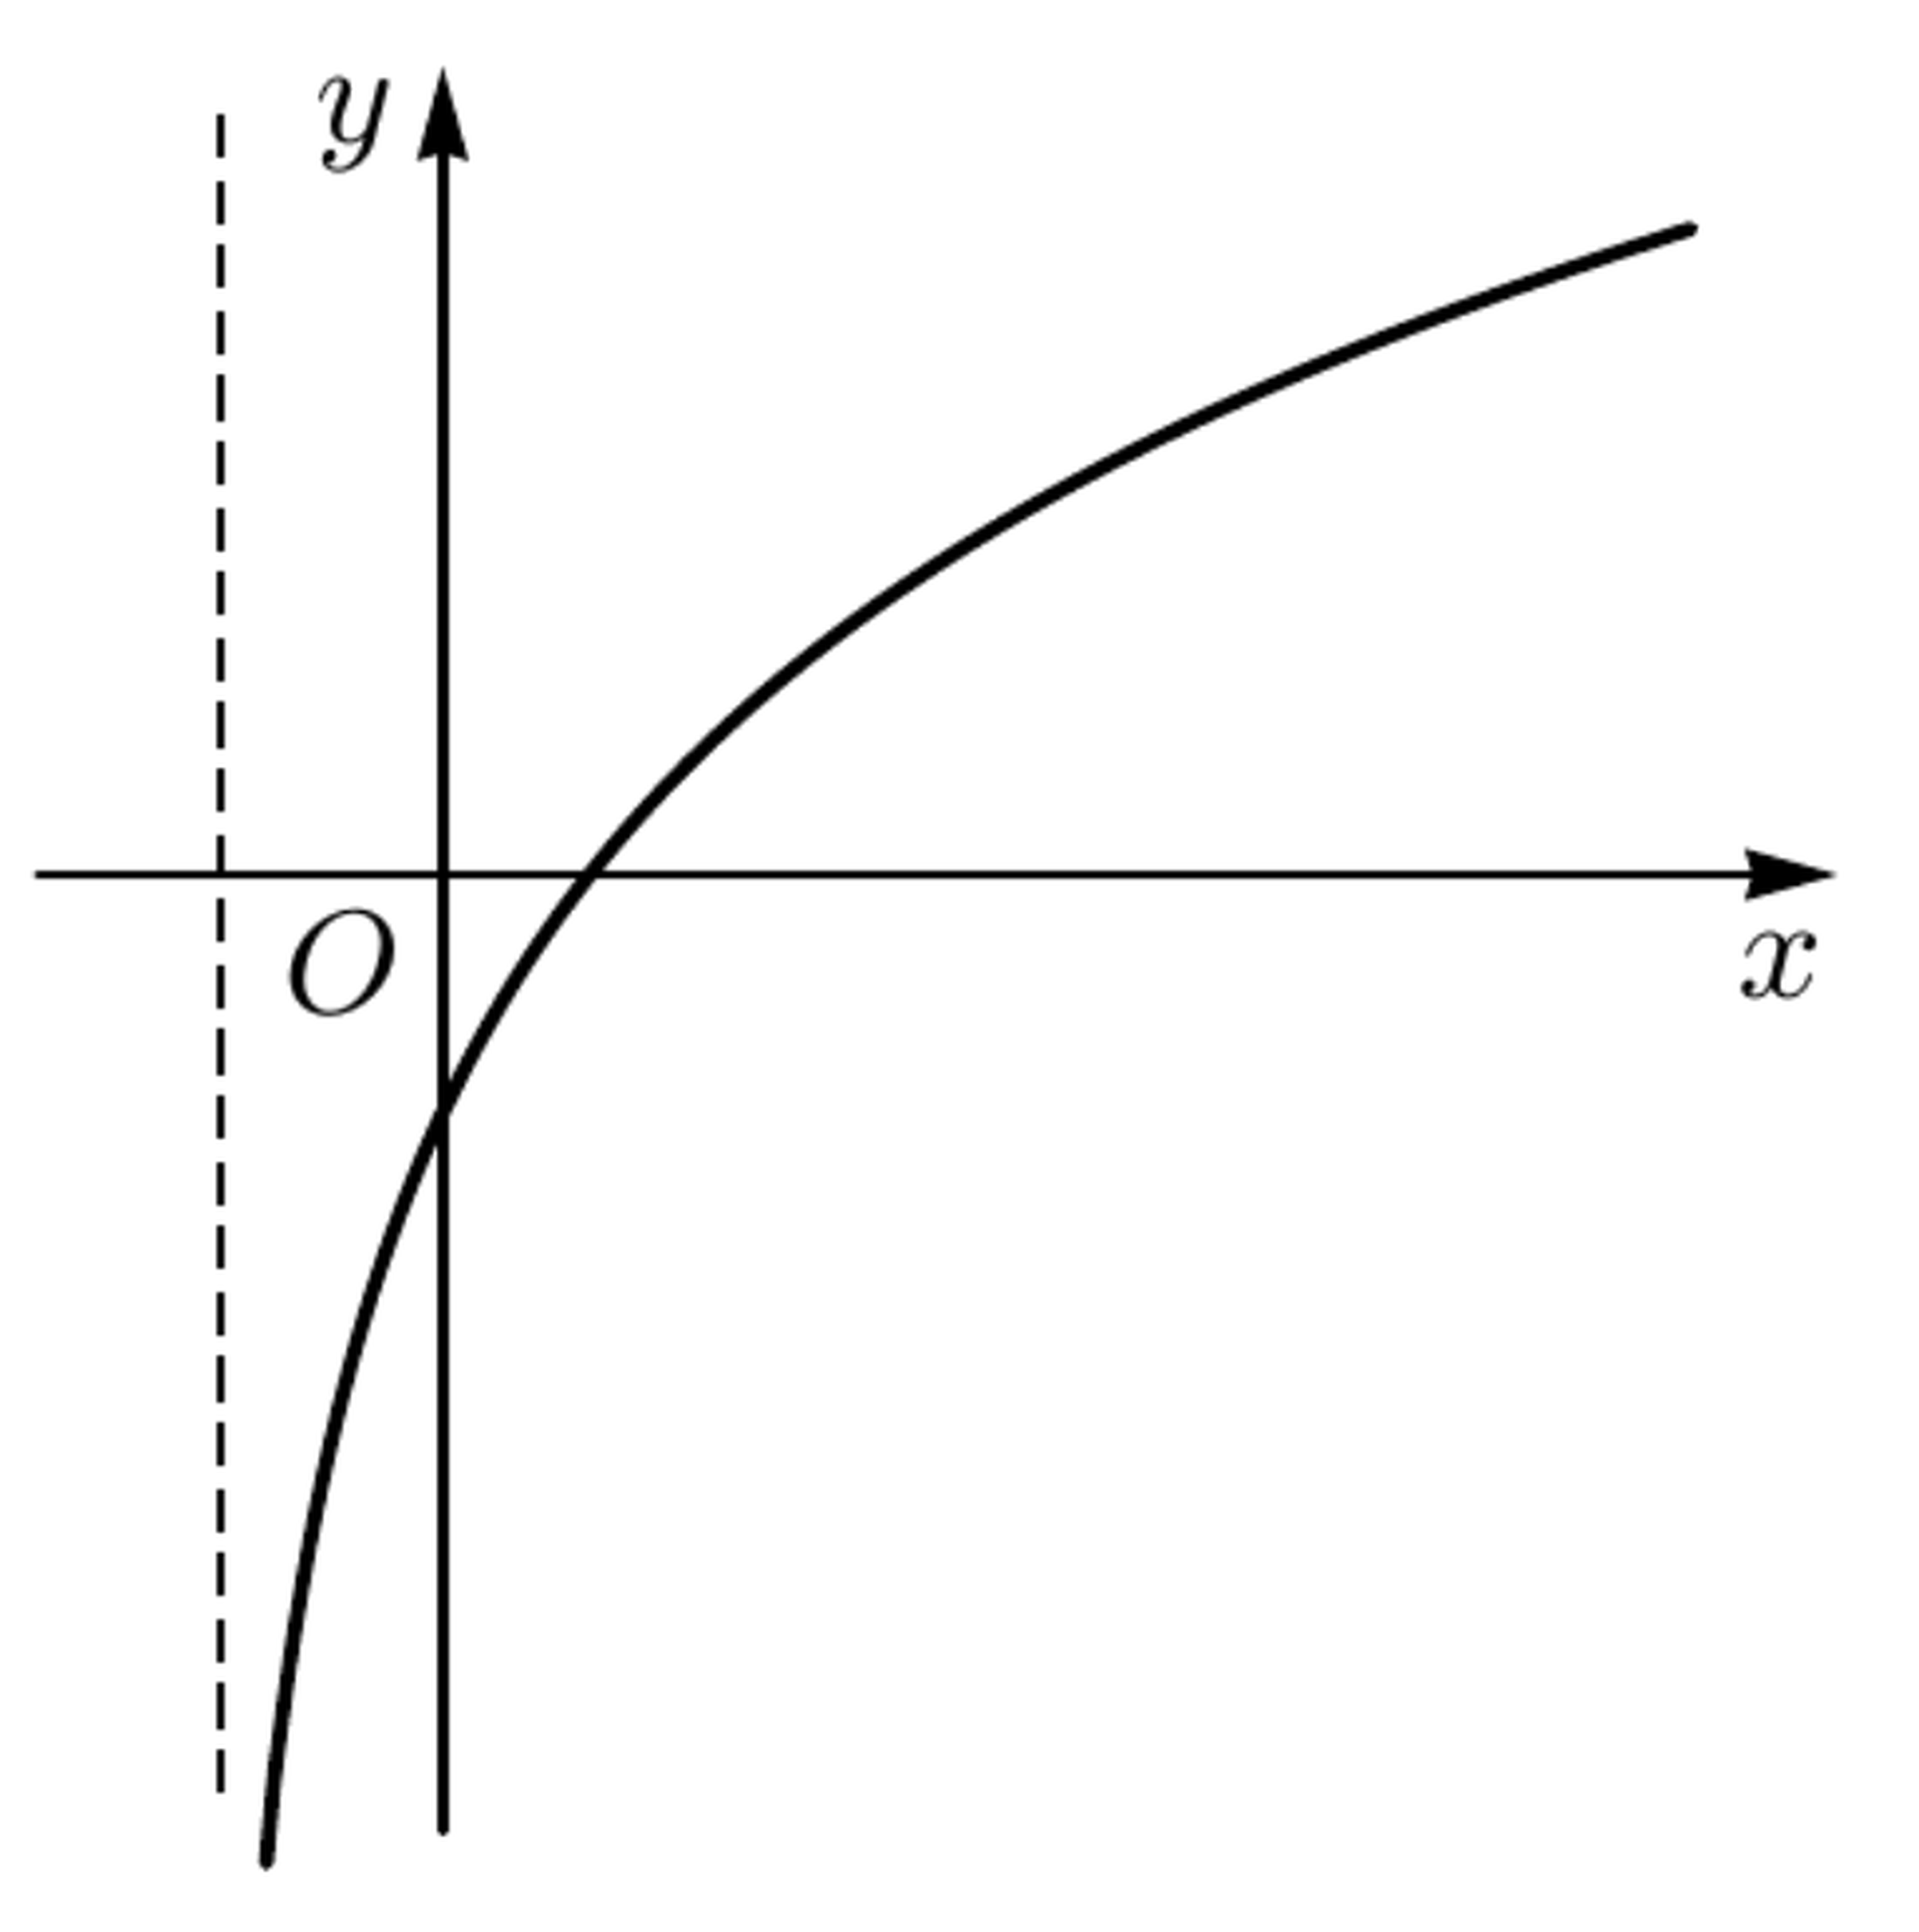
\includegraphics[width=0.42\textwidth]{figures/gao158_q15.png}
\end{center}

\keepwithprev
A. $a>1, b>1$\qquad\qquad B. $a>1, 0<b<1$

C. $0<a<1, b>1$\qquad\qquad D. $0<a<1, 0<b<1$

\ifanswer
\solbegin
\step{图像严格增，得 $a>1$.}
\step{图像与 $y$ 轴交于 $x$ 轴下方，得 $b>0$ 且 $\log_a b<0$，即 $0<b<1$，故选 $B$.}
\solend
\fi

% === Q16 === \lvert\log_2 x\rvert；解析 5 行，故选 C
\item 已知函数 $f(x)=\lvert\log_2 x\rvert$，若 $0<a<b$ 且 $f(a)=f(b)$，则 $a+2b$ 的取值范围是\mbox{（\quad）}

\keepwithprev
A. $(2\sqrt2,+\infty)$\qquad B. $[2\sqrt2,+\infty)$\qquad C. $(3,+\infty)$\qquad D. $[3,+\infty)$

\ifanswer
\solbegin
\step{由 $a<b$ 及 $\lvert\log_2 a\rvert=\lvert\log_2 b\rvert$，得 $\log_2 a=-\log_2 b$，即 $ab=1$，}
\step{且 $0<a<1<b$.}
\step{设 $t=a+2b=2b+\dfrac1b$，则 $t-3=\dfrac{(b-1)(2b-1)}{b}>0$.}
\step{反之，任取 $t>3$，令 $b=\dfrac{t+\sqrt{t^2-8}}{4}>1$、$a=\dfrac1b$，则满足题设且 $a+2b=t$.}
\step{因此取值范围为 $(3,+\infty)$，故选 $C$.}
\solend
\fi

\end{enumerate}

\bigsec{三、解答题}

\begin{enumerate}
\setcounter{enumi}{16}

% === Q17 === 集合、\overline{A}、\subseteq；解析 9 行
\item 已知全集 $U=\R$，集合 $A=\left\{x\mid\dfrac{x-3}{x+1}\leqslant0\right\}$，$B=\{x\mid x^2-2mx+m^2-9<0\}$（$m$ 为实数）.

(1) 当 $m=4$ 时，求 $A\cap B$ 和 $\overline{A}\cup B$；

(2) 若“$x\in A$”是“$x\in B$”的充分条件，求实数 $m$ 的取值范围.

\ifanswer
\solbegin
\step{(1) $\dfrac{x-3}{x+1}\leqslant0\Leftrightarrow-1<x\leqslant3$，所以 $A=(-1,3]$.}
\step{当 $m=4$ 时，$B=\{x\mid(x-4)^2<9\}=(1,7)$，}
\step{于是 $A\cap B=(1,3]$，$\overline{A}\cup B=(-\infty,-1]\cup(1,+\infty)$；}
\step{(2) $x^2-2mx+m^2-9<0\Leftrightarrow(x-m)^2<9$，所以 $B=(m-3,m+3)$.}
\step{题设充分条件等价于 $A\subseteq B$.}
\step{由于 $A=(-1,3]$，左端须满足 $m-3\leqslant-1$.}
\step{又 $3\in A$，须有 $3<m+3$.}
\step{这两个条件也保证 $(-1,3]\subseteq(m-3,m+3)$，}
\step{因此 $A\subseteq B\Leftrightarrow\begin{cases}m-3\leqslant-1\\m+3>3\end{cases}\Leftrightarrow0<m\leqslant2$.}
\solend
\fi

% === Q18 === 蓄水池造价（含 (3) 场地限制）；单位 \mathrm{m}；解析 13 行
\item 某工厂拟建一个容积为 $400\mathrm{m}^3$ 的无盖长方体蓄水池，池深 $4\mathrm{m}$，池底为矩形，其一边长
为 $x\mathrm{m}$. 池壁每平方米造价 100 元，池底每平方米造价 150 元. 设水池的总造价为 $C$
元.

(1) 把 $C$ 表示成 $x$ 的函数，并写出它的定义域；

(2) 当 $x$ 为何值时，总造价最低？最低造价是多少？

(3) 受场地限制，池底一边长 $x$ 不超过 $8\mathrm{m}$，此时总造价最低是多少？

\ifanswer
\solbegin
\step{(1) 设池底另一边长为 $y\mathrm{m}$，则 $4xy=400$，所以 $y=\dfrac{100}{x}$，$x>0$.}
\step{池底面积为 $100\mathrm{m}^2$，池壁总面积为 $8\left(x+\dfrac{100}{x}\right)\mathrm{m}^2$，}
\step{因此 $C(x)=100\times8\left(x+\dfrac{100}{x}\right)+150\times100=800x+\dfrac{80000}{x}+15000$，}
\step{定义域为 $(0,+\infty)$.}
\step{(2) 因为 $x>0$，所以 $C(x)=800\left(x+\dfrac{100}{x}\right)+15000$，}
\step{$\geqslant800\times2\sqrt{x\cdot\dfrac{100}{x}}+15000=31000$，}
\step{当且仅当 $x=\dfrac{100}{x}$，即 $x=10$ 时取等号.}
\step{答：当 $x=10$ 时，总造价最低，为 31000 元.}
\step{(3) 此时定义域为 $(0,8]$. 任取 $0<x_1<x_2\leqslant8$，}
\step{则 $C(x_2)-C(x_1)=800(x_2-x_1)\left(1-\dfrac{100}{x_1x_2}\right)<0$，}
\step{所以 $C(x)$ 在 $(0,8]$ 上严格递减，$x=8$ 时总造价最低，}
\step{且 $C(8)=800\times8+\dfrac{80000}{8}+15000=31400$.}
\step{答：受场地限制时，最低总造价为 31400 元.}
\solend
\fi

% === Q19 === 甲乙滤材 0.8^n／0.7^n；解析 17 行
\item 某环保公司研发了两种新型滤材甲和乙：污水每经过一层甲滤材，污染物含量减少
20\%；每经过一层乙滤材，污染物含量减少 30\%. 每层甲滤材成本 3 万元，每层乙滤材
成本 4 万元. 设原污水中污染物含量为 1，要求处理后污染物含量低于原来的 5\%.

(1) 若只使用一种滤材，污水经过 $n$ 层后污染物含量为 $y$，分别写出使用甲、乙两种滤材
时 $y$ 关于 $n$ 的函数关系式（$n$ 为正整数）；

(2) 若只使用一种滤材，分别求甲、乙至少各需要多少层，并比较哪种滤材的总成本更
低；

(3) 若两种滤材可以混合使用（先后顺序不影响效果），设使用甲滤材 $m$ 层、乙滤材 $n$
层（$m$、$n$ 为非负整数），求满足要求的最低总成本，并指出此时 $m$、$n$ 的值.

\ifanswer
\solbegin
\step{(1) 甲：$y=0.8^n$；乙：$y=0.7^n$，其中 $n$ 为正整数.}
\step{(2) 两种滤材均须满足 $y<0.05$，且污染物含量随层数增加而严格减少.}
\step{$0.8^{14}\approx0.04398<0.05<0.05498\approx0.8^{13}$，}
\step{$0.7^9=0.040353607<0.05<0.05764801=0.7^8$，}
\step{甲至少需要 14 层，成本为 $3\times14=42$ 万元；}
\step{乙至少需要 9 层，成本为 $4\times9=36$ 万元.}
\step{因此，只使用一种滤材时，使用乙滤材的总成本更低.}
\step{(3) 设总成本为 $C$ 万元，则 $C=3m+4n,0.8^m\cdot0.7^n<0.05,m,n\in\{0,1,2,\cdots\}$，}
\step{若 $m\geqslant3$，将其中 3 层甲替换为 2 层乙，}
\step{因为 $0.7^2=0.49<0.512=0.8^3,2\times4<3\times3$，}
\step{替换后污染物含量更低，成本减少 1 万元，因此最低成本方案必有 $m\leqslant2$.}
\step{当 $m=0$ 时，由第（2）小题得至少需要 9 层乙，最低成本为 36 万元.}
\step{当 $m=1$ 或 $m=2$ 时，$0.8\cdot0.7^7>0.8^2\cdot0.7^7=0.052706752>0.05$，}
\step{$0.8^2\cdot0.7^8<0.8\cdot0.7^8=0.046118408<0.05$，}
\step{因此两种情形均至少需要 8 层乙，}
\step{对应最低成本分别为 $3+4\times8=35$ 万元，$3\times2+4\times8=38$ 万元.}
\step{答：满足要求的最低总成本为 35 万元，此时使用甲滤材 1 层、乙滤材 8 层.}
\solend
\fi

% === Q20 === f(x)=\log_2(4^x+1)-x；\Delta；解析 17 行
\item 已知函数 $f(x)=\log_2(4^x+1)-x$.

(1) 证明 $f(x)=\log_2(2^x+2^{-x})$，并求 $f(x)$ 的最小值及取得最小值时 $x$ 的值；

(2) 解不等式 $f(x)>\log_2 5-1$；

(3) 证明：函数 $f(x)$ 在区间 $[0,+\infty)$ 上是严格增函数；并求使关于 $x$ 的方程 $f(x)=m$ 恰
有两个不同实数解的实数 $m$ 的取值范围.

\ifanswer
\solbegin
\step{(1) $f(x)=\log_2(4^x+1)-\log_2 2^x=\log_2\dfrac{4^x+1}{2^x}=\log_2(2^x+2^{-x})$，}
\step{因为 $2^x+2^{-x}\geqslant2\sqrt{2^x\cdot2^{-x}}=2$，所以 $f(x)\geqslant\log_2 2=1$，}
\step{等号当且仅当 $2^x=2^{-x}$，即 $x=0$ 时成立，故最小值为 1.}
\step{(2) 令 $t=2^x>0$，则 $f(x)>\log_2 5-1\Leftrightarrow t+\dfrac1t>\dfrac52\Leftrightarrow2t^2-5t+2>0$}
\step{$\Leftrightarrow(2t-1)(t-2)>0$，}
\step{结合 $t>0$，得 $0<t<\dfrac12$ 或 $t>2$，即 $x<-1$ 或 $x>1$，}
\step{解集为 $(-\infty,-1)\cup(1,+\infty)$.}
\step{(3) 任取 $0\leqslant x_1<x_2$，记 $a=2^{x_1}$，$b=2^{x_2}$，则 $1\leqslant a<b$，$ab>1$，}
\step{从而 $\left(b+\dfrac1b\right)-\left(a+\dfrac1a\right)=(b-a)\left(1-\dfrac{1}{ab}\right)>0$，}
\step{由对数函数的严格递增性，得 $f(x_1)<f(x_2)$，}
\step{所以 $f(x)$ 在 $[0,+\infty)$ 上是严格增函数.}
\step{当 $m<1$ 时，由（1）得方程无实数解；当 $m=1$ 时，只有实数解 $x=0$.}
\step{当 $m>1$ 时，令 $t=2^x>0$，则 $f(x)=m\Leftrightarrow t+\dfrac1t=2^m\Leftrightarrow t^2-2^m t+1=0$，}
\step{此时 $\Delta=2^{2m}-4>0$，两根之和为 $2^m>0$、之积为 $1>0$，}
\step{故有两个不同的正根.}
\step{每个正根 $t$ 唯一确定一个实数 $x=\log_2 t$，故原方程恰有两个不同实数解，}
\step{所求范围为 $m\in(1,+\infty)$.}
\solend
\fi

% === Q21 === f(x)=4^x-m\cdot2^{x+1}+3 值域与 h(m) 分段；解析 13 行
\item 已知函数 $f(x)=4^x-m\cdot2^{x+1}+3$（$m\in\R$），$x\in[0,2]$.

(1) 当 $m=1$ 时，求 $f(x)$ 的值域；

(2) 记 $f(x)$ 的最小值为 $h(m)$，求 $h(m)$ 的表达式；

(3) 若关于 $x$ 的方程 $f(x)=0$ 在区间 $[0,2]$ 上有解，求实数 $m$ 的取值范围.

\ifanswer
\solbegin
\step{令 $t=2^x$，则 $t\in[1,4]$，且 $f(x)=t^2-2mt+3=(t-m)^2+3-m^2$，}
\step{(1) 当 $m=1$ 时，$f(x)=(t-1)^2+2$.}
\step{由 $0\leqslant t-1\leqslant3$，得 $2\leqslant f(x)\leqslant11$，值域为 $[2,11]$.}
\step{(2) 二次函数 $y=(t-m)^2+3-m^2$ 的对称轴为直线 $t=m$.}
\step{当 $m\leqslant1$ 时，在 $t=1$ 处取最小值；}
\step{当 $1<m<4$ 时，在 $t=m$ 处取最小值；}
\step{当 $m\geqslant4$ 时，在 $t=4$ 处取最小值；}
\step{因此 $h(m)=\begin{cases}4-2m,&m\leqslant1\\3-m^2,&1<m<4\\19-8m,&m\geqslant4\end{cases}$；}
\step{(3) 方程 $f(x)=0$ 在 $[0,2]$ 上有解，}
\step{等价于存在 $t\in[1,4]$，使 $m=\dfrac{t^2+3}{2t}=\dfrac12\left(t+\dfrac3t\right)$，}
\step{由基本不等式，$m\geqslant\dfrac12\cdot2\sqrt{t\cdot\dfrac3t}=\sqrt3$，当且仅当 $t=\sqrt3$ 时取等号；}
\step{又 $\dfrac{19}{8}-m=\dfrac{(4-t)(4t-3)}{8t}\geqslant0$，当且仅当 $t=4$ 时取等号；}
\step{因此必有 $\sqrt3\leqslant m\leqslant\dfrac{19}{8}$.}
\solend
\fi

\end{enumerate}

\end{document}
"
%
% ① 原始材料：微信公众号"魔都数学加油站"文章，连载"27学年高一158"，原文标题
% "27学年高一158——2026-2027年上海市上实东滩高一上期中"（本卷本地编号 158 与
% 原卷连载号一致，无撞号）。
% 正文为 9 张 PNG 页（01/05/08/09 为 2560×3620，02/03/04/06/07 为 4762×6735，
% 同一篇各页分辨率混排，逐页按各自分辨率裁图核对）。
% 体例：讲评版——填空 3—12（10 题）、选择 13—16（4 题）、解答 17—21（5 题），
% 共 19 题，自第 3 题起编（1、2 未印在本篇）；Q5 只印【答案】、其余 18 题
% 逐题印【解析】（逐题核实，见 ②）。题目、答案、解析均据原图转录；卷面粉红色
% 水印"魔都数学加油站"及公众号页脚未录入。全卷末题为第 21 题，无附加题节。
% 全卷 2 组配图（逐页通读 9 页确认）——
%   · Q10 题干右侧"曼 → man"字形变换图（02 页），题目配图、三版都出，
%     裁 figures/gao158_q10.png；
%   · Q15 题干"如图所示"对数函数大致图像（03 页右下），题目配图、三版都出，
%     裁 figures/gao158_q15.png；
% 2 图均取自原卷截图，去粉色水印、转灰度、4× LANCZOS 放大；
% 其余各页逐页确认无其它题目配图、无解析内配图、无表格。
%
% 卷首标题：原卷印作"2026-2027 年上实东滩高一上期中"，年份区间按全稿惯例排 en dash；
% 原卷卷面未印副标题，本稿按同期中卷知识模块口径补出"集合与常用逻辑用语、不等式、函数"。
%
% ② 与原卷的排版差异／照录项清单：
%   ① 原文从第 3 题起，本稿保留原题号；共 19 题三节，解答题 5 题到 21；
%      三节各自一个 enumerate＋各自 \setcounter{enumi}{2}／{12}／{16}，
%      不贯穿（题目溯源.py 按 \bigsec 切节、每节独立计 depth，只收 depth==1 的 \item）；
%   ② 混合体例：Q5 只印【答案】、无【解析】，按 高一156 第 3 题成例另提
%      \ans{}、不补造解析；其余 18 题印【解析】、用 \solbegin…\solend；
%      四道选择题答案均在解析末句"故选 C／B／B／C"（逐个放大复核）、
%      题干括号 \mbox{（\quad）} 留空、不另提 \ans{}；答案版
%      【答案】/【解析】标记数 = 19 = 全卷题数（1 个 \ans ＋ 18 个 \solbegin）；
%   ③ 原卷卷面未印副标题，本稿按知识模块口径补出；
%   ④ 原卷填空横线按全稿惯例排 \blankline[4.4em]；选择题选项段前按惯例各加
%      \keepwithprev；解答题不留作答区、不加 \anspace（原卷为讲评版）；
%   ⑤ 数集：Q13"在 \R 上严格递增"、Q14"$x\in\R$"、Q17"$U=\R$"、
%      Q21"$m\in\R$" 原卷印正体粗体 R，按全稿惯例归一 \R；
%      绝对值排 \lvert…\rvert（Q12 $\lvert a\rvert$、Q14 $\lvert x-2\rvert$、
%      Q16 $\lvert\log_2 x\rvert$／$\lvert\log_2 a\rvert$／$\lvert\log_2 b\rvert$），
%      集合描述竖线排 \mid（Q17），不等号按全稿惯例排 \leqslant／\geqslant，
%      补集上划线 \overline{A}（Q17）；
%   ⑥ 子集／真子集符号逐处照录不统一：Q14 解析"$(2,3)\subsetneq(1,3)$"原卷印
%      带下划线且被斜杠划过的 ⊊（真子集，放大 03 页确认），照录 \subsetneq；
%      Q17 解析三处"$A\subseteq B$""$(-1,3]\subseteq(m-3,m+3)$"原卷印
%      带下划线 ⊆（放大 05 页确认），照录 \subseteq；本卷无单线 \subset 用例；
%   ⑦ 判别式：Q20 (3) 解析"$\Delta=2^{2m}-4>0$"原卷印高瘦等腰 \Delta
%      （像素实测高/宽 ≈ 1.13，扁三角 \triangle 为 0.93，放大 08 页确认），
%      照录 \Delta；本卷无扁三角 \triangle 用例；
%   ⑧ "图像"与"图象"：全卷统一用"图像"（Q6 题干、Q10 两处、Q11 解析、
%      Q15 题干与解析两处，逐处放大确认带单人旁），照录不改；
%   ⑨ 中文弯引号照录：Q5 命题"若实数…"、Q10"曼""man""新"、Q14 题干与
%      解析的两则不等式、Q17 (2)"$x\in A$""$x\in B$"；注释里一律 ASCII 引号；
%   ⑩ 半角逗号逐处照录：Q8"$2,3,4$""$-2,-1,0$"、Q10 点坐标 $(x,y)$／
%      $(t,2^t-1)$／$(1-2^t,t)$、Q15 四选项"$a>1, b>1$"等、
%      Q19 (3)"$C=3m+4n,0.8^m\cdot0.7^n<0.05,m,n\in\{0,1,2,\cdots\}$"
%      与"$0.7^2=0.49<0.512=0.8^3,2\times4<3\times3$"、
%      Q21 cases 内"$4-2m,$"等；其余行中逗号／顿号照录全角；
%      行末西文句点 ASCII `.`；
%   ⑪ 顿号照录：Q3"（用 $a$、$b$ 表示）"、Q5"$x$、$y$"、Q13"A、B"、
%      Q16 解析"$>1$、$a=\dfrac1b$"、Q19"甲、乙""$m$、$n$"、
%      Q20"$2^m>0$、之积为"、Q21"$m$、$n$"；顿号一律移到数学模式外，
%      数学模式内不出现中文标点；
%   ⑫ 角度与单位照录：Q10 三处"$90^{\circ}$"、Q18"$400\mathrm{m}^3$"
%      "$4\mathrm{m}$""$x\mathrm{m}$""$8\mathrm{m}$""$y\mathrm{m}$"
%      "$100\mathrm{m}^2$""$\left(x+\dfrac{100}{x}\right)\mathrm{m}^2$"；
%      Q19 百分号"20\%""30\%""5\%"按原卷排 \%；
%   ⑬ 文本模式全角括号照录：Q10"（提示：…）"、Q17"（$m$ 为实数）"、
%      Q19"（$n$ 为正整数）""（先后顺序不影响效果）""（$m$、$n$ 为非负整数）"、
%      Q20"由（1）得"、Q19"由第（2）小题"、Q21"（$m\in\R$）"；
%      子题行首标号按全稿惯例用半角 (1)(2)(3)；
%   ⑭ 复杂式照录别简化：Q3 $\dfrac{\log_3 2+\log_3 5}{\log_3 3+2\log_3 2}$、
%      Q8 $[-3,-2)\cup(4,5]$、Q9 $18ab=2^t\cdot3^t=6^t=a+b$、
%      Q12 $\dfrac{\sqrt6}{2}$、Q18 $C(8)=800\times8+\dfrac{80000}{8}+15000=31400$
%      （原卷即 C(8)，非 C(2)）、Q19 $0.8^{14}\approx0.04398$、
%      $0.7^9=0.040353607$、$0.052706752$、$0.046118408$、
%      Q20 $t^2-2^m t+1=0$、Q21 $h(m)$ 三段 cases 与 $\dfrac{(4-t)(4t-3)}{8t}$ 等；
%      \left…\right 不得拆到不同 $…$ 组；cases 块整体算一个印刷行；
%   ⑮ 一条 \step = 原卷解析的一个印刷行；别并折行、别拆行。跨页续印按题合并
%      （Q7 的 01—02 页、Q9/Q10/Q11 的 02—03 页、Q13/Q14 的 03 页上下、
%      Q15/Q16 的 04 页上下、Q17 的 04—05 页、Q18 的 05—06 页、
%      Q19 的 06—07 页、Q20 的 07—08 页、Q21 的 08—09 页）；
%      跨半页重叠行（Q5【答案】、Q9 设公共值行、Q10 题干、Q16 反之行、
%      Q18 (2) 题干、Q19 末两行、Q20 (3) 末行、Q21 cases 块）只算一个印刷行；
%   ⑯ 配图：2 组题目配图（见 ①），均三版都出，\needvspace 守卫放 \item 之前
%      把"题干＋图"整块推走，\includegraphics 放题干之后；本卷无解析内配图、
%      无红字加粗小标题（全卷逐页确认，故无 \stepm）。
%
% ③ 行数复核：一条 \step = 原卷解析的一个印刷行，cases 块作一个印刷行计。
%   逐题数（逐页核对）：Q3：1；Q4：2；Q5：0（只印【答案】、提 \ans{}，
%   不计入 \step 账）；Q6：1；Q7：4；Q8：5；Q9：2；Q10：2；Q11：3；
%   Q12：3；Q13：2；Q14：3；Q15：2；Q16：5；Q17：9；Q18：13；
%   Q19：17；Q20：17；Q21：13。
%   合计 104 行（104 条 \step ＋ 0 条 \stepm），与原卷逐题印刷行相等。
%   全卷 19 题：Q5 一处 \ans{} ＋ 其余 18 题设 \solbegin…\solend，
%   答案版【答案】/【解析】标记数 = 19 = 全卷题数。
%
% ④ 页码分布（供回原图复核）：
%   卷首标题＋"一、填空题"＋Q3 题干＋解析 1 行、Q4 题干＋解析 2 行、
%   Q5 题干＋【答案】在 01 页上半；Q5【答案】（重叠重印）＋Q6 题干＋解析 1 行、
%   Q7 题干＋解析前 3 行在 01 页下半；Q7 解析末行＋Q8 题干＋解析 5 行、
%   Q9 题干＋解析首行在 02 页上半；Q9 解析末行＋Q10 题干（含"曼→man"图）
%   ＋解析 2 行＋Q11 题干＋解析首行在 02 页下半；Q11 解析后 2 行＋Q12 题干
%   ＋解析 3 行＋"二、选择题"标题＋Q13 题干＋选项在 03 页上半；
%   Q13 选项（重叠重印）＋解析 2 行＋Q14 题干＋选项＋解析 3 行＋Q15 题干
%   ＋对数图像（右侧）在 03 页下半；Q15 选项＋解析 2 行＋Q16 题干＋选项
%   ＋解析前 4 行在 04 页上半；Q16 解析末行＋"三、解答题"标题＋Q17 题干
%   ＋两问＋解析 (1) 3 行在 04 页下半；Q17 解析 (2) 6 行＋Q18 题干＋三问
%   ＋解析 (1) 4 行＋(2) 首行在 05 页上下；Q18 解析 (2) 后 3 行＋(3) 5 行
%   ＋Q19 题干＋三问＋解析 (1) 1 行＋(2) 3 行在 06 页上下；Q19 解析 (2) 3 行
%   ＋(3) 12 行在 07 页上半；Q19 解析末 2 行（重叠）＋Q20 题干＋三问
%   ＋解析 (1) 3 行在 07 页下半；Q20 解析 (2) 4 行＋(3) 前 4 行在 08 页上半；
%   Q20 解析 (3) 后 6 行＋Q21 题干＋(1) 问在 08 页下半；Q21 (2)(3) 问＋
%   解析 (1) 3 行＋(2) 5 行＋cases 块在 09 页上半；Q21 cases 块（重叠）
%   ＋(3) 解析 5 行在 09 页下半。本稿按题连排，不丢行、不并折行；
%   全卷末题为第 21 题，无附加题节。
%
% ⑤ 存疑／需主会话回原图复核：
%   1. Q14 解析"$(2,3)\subsetneq(1,3)$"的 ⊊（真子集带斜杠）与 Q17 的 ⊆
%      是两种不同记号，本稿分别照录 \subsetneq／\subseteq，请复核；
%   2. Q20 (3)"$\Delta=2^{2m}-4>0$"判为高瘦 \Delta，请复核是否 \triangle；
%   3. 任务书提示"Q18 解析里印 C(2)=…"，但 06 页原图逐处读作
%      $C(8)=800\times8+\dfrac{80000}{8}+15000=31400$，未找到 C(2)，
%      本稿照原卷排 C(8)，请复核；
%   4. Q19 解析末句"最低总成本为 35 万元"（07 页上下两处印同），
%      OCR 曾误读为 34，本稿按 35 照录，请复核；
%   5. Q10 提示末尾"坐标为 $(-y,x)$）."为半角 $)$＋全角 $）$ 两枚括号，
%      本稿照录，请复核；
%   6. Q21 cases 块后"；"落在分式中行右侧（排版居中基线所致），
%      本稿排作 $…\end{cases}$；，请复核。
%   全卷除此 6 类外未发现其它笔误／自相矛盾处；19 题中 18 题印【解析】。
%
\documentclass[a4paper,11pt]{article}
\usepackage{common}

\begin{document}

\examtitlest[3]{2026--2027 年上实东滩高一上期中}{集合与常用逻辑用语、不等式、函数}

\bigsec{一、填空题}

\begin{enumerate}
\setcounter{enumi}{2}

% === Q3 === 换底公式；解析 1 行
\item 已知 $3^a=5$，$\log_3 2=b$，则 $\log_{12} 10=$\blankline[4.4em]（用 $a$、$b$ 表示）.

\ifanswer
\solbegin
\step{$\log_{12} 10=\dfrac{\log_3 2+\log_3 5}{\log_3 3+2\log_3 2}=\dfrac{a+b}{1+2b}$.}
\solend
\fi

% === Q4 === 定义域；解析 2 行；半角括号 ( ) 与全角逗号照录
\item 函数 $y=\sqrt{2-x}+\lg(x^2-1)$ 的定义域为\blankline[4.4em].

\ifanswer
\solbegin
\step{由 $2-x\geqslant0$ 且 $x^2-1>0$，得 $x\leqslant2$ 且 ($x<-1$或$x>1$)，}
\step{定义域为 $(-\infty,-1)\cup(1,2]$.}
\solend
\fi

% === Q5 === 只印【答案】、无【解析】；反证法，中文弯引号
\item 用反证法证明命题“若实数 $x$、$y$ 满足 $x+y>2$，则 $x$、$y$ 中至少有一个大于 1”时，
应假设\blankline[4.4em].

\ifanswer
\ans{$x\leqslant1$ 且 $y\leqslant1$}
\fi

% === Q6 === 图像平移；解析 1 行
\item 函数 $y=\dfrac{2x+1}{x-1}$ 的图像可由函数 $y=\dfrac{3}{x}$ 的图像先向右平移 $a$ 个单位，再向上平移 $b$ 个单位
得到，则 $a+b=$\blankline[4.4em].

\ifanswer
\solbegin
\step{$y=\dfrac{2x+1}{x-1}=\dfrac{3}{x-1}+2$，所以 $a=1$，$b=2$，$a+b=3$.}
\solend
\fi

% === Q7 === 集合三元子集；解析 4 行，跨 01—02 页
\item 设 $A=\{a_1,a_2,a_3,a_4\}$ 是由四个实数组成的集合，若 $A$ 的所有三元子集中，三个元素之和
组成的集合为 $B=\{1,4,7,12\}$，则集合 $A=$\blankline[4.4em].

\ifanswer
\solbegin
\step{设 $S=a_1+a_2+a_3+a_4$，}
\step{每个元素在四个三元子集中恰出现三次，则 $3S=1+4+7+12=24$，得 $S=8$.}
\step{四个三元子集的元素和分别为 $S-a_i$，}
\step{所以 $A=\{8-1,8-4,8-7,8-12\}=\{-4,1,4,7\}$.}
\solend
\fi

% === Q8 === 不等式整数解；解析 5 行；半角逗号照录
\item 不等式 $x^2-(a+1)x+a<0$ 的解集中恰有 3 个整数，则 $a$ 的取值范围是\blankline[4.4em].

\ifanswer
\solbegin
\step{原不等式为 $(x-1)(x-a)<0$；}
\step{$a=1$ 时解集为空集，不符合题意.}
\step{若 $a>1$，解集为 $(1,a)$，恰含整数 $2,3,4$，则 $4<a\leqslant5$.}
\step{若 $a<1$，解集为 $(a,1)$，恰含整数 $-2,-1,0$，则 $-3\leqslant a<-2$.}
\step{故 $a$ 的取值范围是 $[-3,-2)\cup(4,5]$.}
\solend
\fi

% === Q9 === 对数换底＋指数；解析 2 行
\item 已知正数 $a$、$b$ 满足 $1+\log_2 a=2+\log_3 b=\log_6(a+b)$，则 $\dfrac1a+\dfrac1b=$\blankline[4.4em].

\ifanswer
\solbegin
\step{设公共值为 $t$，则 $2a=2^t$，$9b=3^t$，$a+b=6^t$，}
\step{于是 $18ab=2^t\cdot3^t=6^t=a+b$，即 $\dfrac1a+\dfrac1b=\dfrac{a+b}{ab}=18$.}
\solend
\fi

% === Q10 === "曼"字旋转 90°；题目配图（三版都出）；解析 2 行
\needvspace{6cm}
\item 网上流传一个有趣的字形变换：把汉字“曼”的右半部分旋转 $90^{\circ}$，就得到英文单词
“man”的艺术字. 数学中，把曲线绕原点旋转也会得到“新”的曲线：将函数
$y=2^x-1$ 的图像绕坐标原点 $O$ 逆时针旋转 $90^{\circ}$，得到的曲线恰是某个函数的
图像，则这个函数的解析式为\blankline[4.4em]（提示：点 $(x,y)$ 绕 $O$ 逆时针旋转 $90^{\circ}$ 后的
坐标为 $(-y,x)$）.

\begin{center}

\includegraphics[width=0.42\textwidth]{figures/gao158_q10.png}
\end{center}

\ifanswer
\solbegin
\step{原图像上的点 $(t,2^t-1)$ 旋转后为 $(1-2^t,t)$.}
\step{记其为 $(x,y)$，则 $x=1-2^y$，即 $y=\log_2(1-x)$，定义域为 $(-\infty,1)$.}
\solend
\fi

% === Q11 === 值域；解析 3 行，跨 02—03 页
\item 函数 $f(x)=\sqrt{x-2}-\sqrt{15-3x}$ 的值域为\blankline[4.4em].

\ifanswer
\solbegin
\step{由 $x-2\geqslant0$ 且 $15-3x\geqslant0$，得定义域为 $[2,5]$.}
\step{在 $[2,5]$ 上，$\sqrt{x-2}$ 与 $-\sqrt{15-3x}$ 均严格递增，因此 $f(x)$ 严格递增.}
\step{$f(2)=-3$，$f(5)=\sqrt3$，结合函数的图像，值域为 $[-3,\sqrt3]$.}
\solend
\fi

% === Q12 === 绝对值 \lvert…\rvert；解析 3 行
\item 设实数 $a$ 满足 $a<4a^3-5a<\lvert a\rvert$，则 $a$ 的取值范围是\blankline[4.4em].

\ifanswer
\solbegin
\step{由 $a<\lvert a\rvert$ 得 $a<0$，原不等式为 $a<4a^3-5a<-a$.}
\step{同除以 $a<0$，得 $1>4a^2-5>-1\Leftrightarrow1<a^2<\dfrac32$，结合 $a<0$，}
\step{得 $-\dfrac{\sqrt6}{2}<a<-1$，故解集为 $\left(-\dfrac{\sqrt6}{2},-1\right)$.}
\solend
\fi

\end{enumerate}

\bigsec{二、选择题}

\begin{enumerate}
\setcounter{enumi}{12}

% === Q13 === \R 归一；解析 2 行，故选 C
\item 已知 $a>b$，则下列不等式一定成立的是\mbox{（\quad）}

\keepwithprev
A. $\dfrac1a<\dfrac1b$\qquad B. $a^2>b^2$\qquad C. $a^3>b^3$\qquad D. $ac^2>bc^2$

\ifanswer
\solbegin
\step{幂函数 $y=x^3$ 在 $\R$ 上严格递增，$a>b\Rightarrow a^3>b^3$，C 正确.}
\step{取 $a=1$，$b=-1$ 得 A、B 不成立；取 $c=0$ 得 D 不成立；故选 $C$.}
\solend
\fi

% === Q14 === \subsetneq 真子集；解析 3 行，故选 B
\item 设 $x\in\R$，则“$\lvert x-2\rvert<1$”是“$x^2-5x+6<0$”的\mbox{（\quad）}

\keepwithprev
A. 充分非必要条件\qquad\qquad B. 必要非充分条件

C. 充要条件\qquad\qquad D. 既非充分又非必要条件

\ifanswer
\solbegin
\step{$\lvert x-2\rvert<1\Leftrightarrow1<x<3$，$x^2-5x+6<0\Leftrightarrow(x-2)(x-3)<0\Leftrightarrow2<x<3$.}
\step{由 $(2,3)\subsetneq(1,3)$，得“$\lvert x-2\rvert<1$”是“$x^2-5x+6<0$”的必要非充分条件，}
\step{故选 $B$.}
\solend
\fi

% === Q15 === 对数函数大致图像（题目配图，三版都出）；解析 2 行，故选 B
\needvspace{9cm}
\item 已知函数 $f(x)=\log_a(x+b)$（$a>0$ 且 $a\ne1$）的大致图像如图所示，则 $a$、$b$ 满足
的关系是\mbox{（\quad）}

\begin{center}
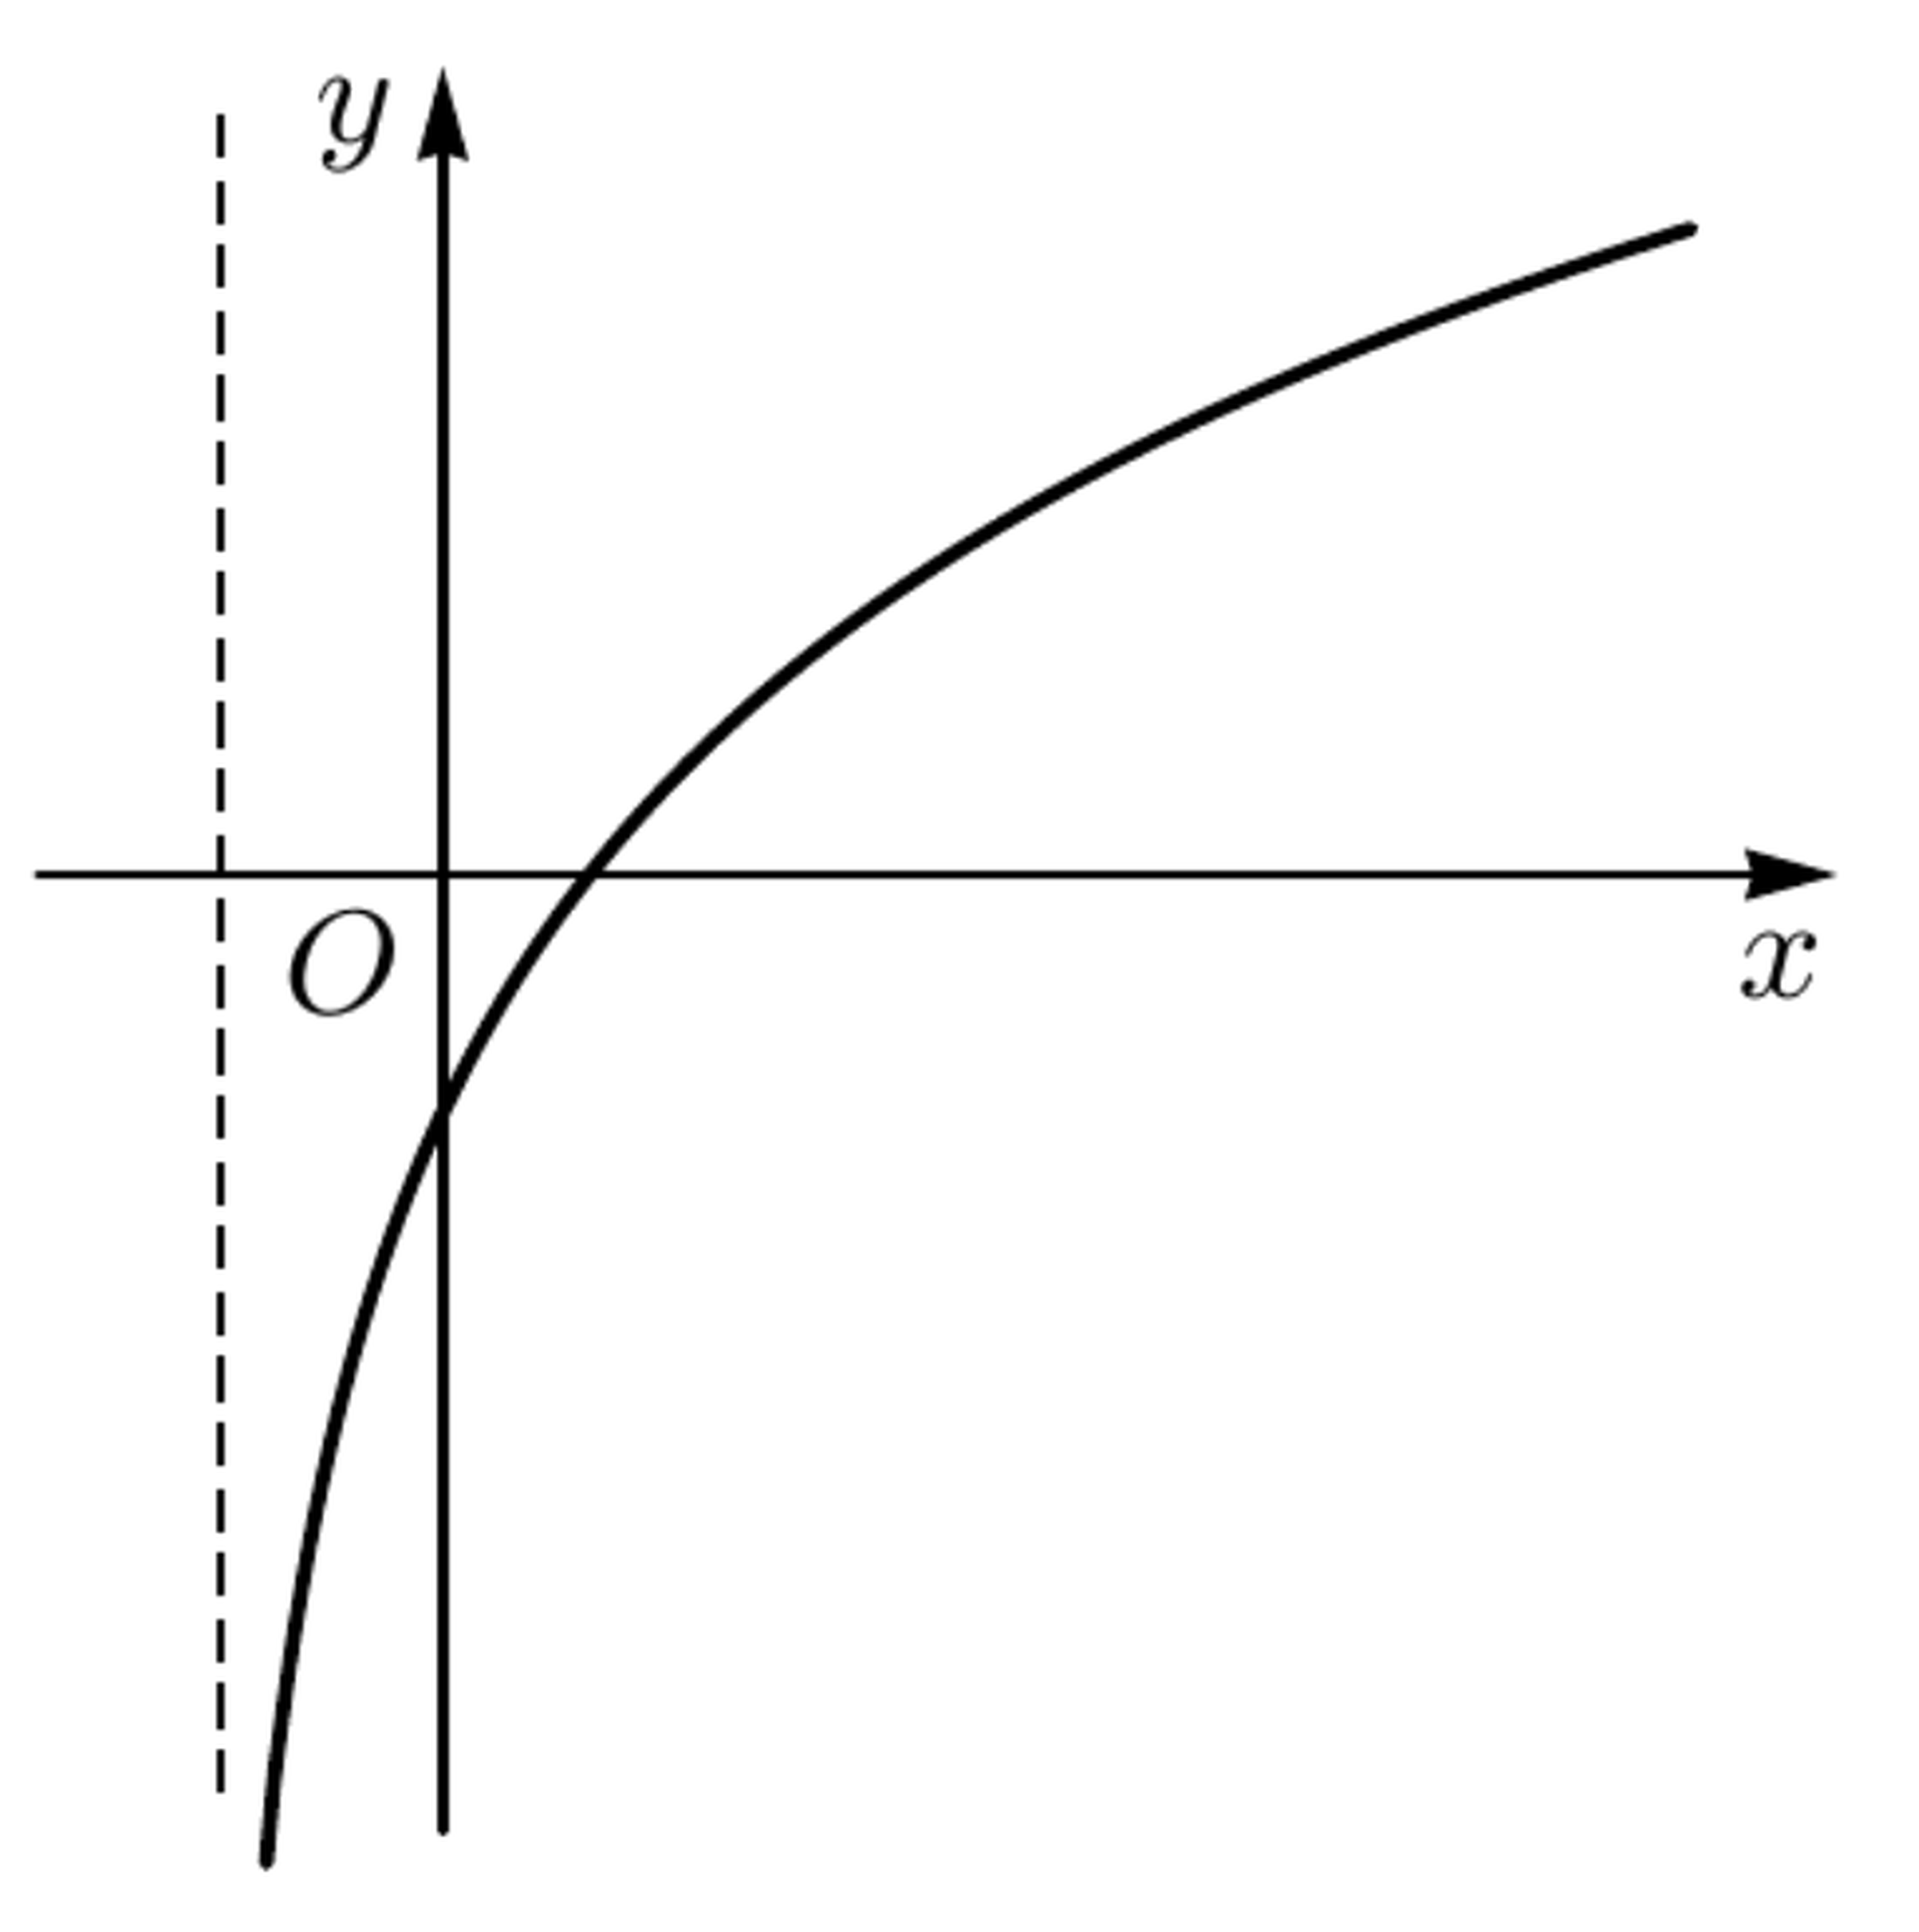
\includegraphics[width=0.42\textwidth]{figures/gao158_q15.png}
\end{center}

\keepwithprev
A. $a>1, b>1$\qquad\qquad B. $a>1, 0<b<1$

C. $0<a<1, b>1$\qquad\qquad D. $0<a<1, 0<b<1$

\ifanswer
\solbegin
\step{图像严格增，得 $a>1$.}
\step{图像与 $y$ 轴交于 $x$ 轴下方，得 $b>0$ 且 $\log_a b<0$，即 $0<b<1$，故选 $B$.}
\solend
\fi

% === Q16 === \lvert\log_2 x\rvert；解析 5 行，故选 C
\item 已知函数 $f(x)=\lvert\log_2 x\rvert$，若 $0<a<b$ 且 $f(a)=f(b)$，则 $a+2b$ 的取值范围是\mbox{（\quad）}

\keepwithprev
A. $(2\sqrt2,+\infty)$\qquad B. $[2\sqrt2,+\infty)$\qquad C. $(3,+\infty)$\qquad D. $[3,+\infty)$

\ifanswer
\solbegin
\step{由 $a<b$ 及 $\lvert\log_2 a\rvert=\lvert\log_2 b\rvert$，得 $\log_2 a=-\log_2 b$，即 $ab=1$，}
\step{且 $0<a<1<b$.}
\step{设 $t=a+2b=2b+\dfrac1b$，则 $t-3=\dfrac{(b-1)(2b-1)}{b}>0$.}
\step{反之，任取 $t>3$，令 $b=\dfrac{t+\sqrt{t^2-8}}{4}>1$、$a=\dfrac1b$，则满足题设且 $a+2b=t$.}
\step{因此取值范围为 $(3,+\infty)$，故选 $C$.}
\solend
\fi

\end{enumerate}

\bigsec{三、解答题}

\begin{enumerate}
\setcounter{enumi}{16}

% === Q17 === 集合、\overline{A}、\subseteq；解析 9 行
\item 已知全集 $U=\R$，集合 $A=\left\{x\mid\dfrac{x-3}{x+1}\leqslant0\right\}$，$B=\{x\mid x^2-2mx+m^2-9<0\}$（$m$ 为实数）.

(1) 当 $m=4$ 时，求 $A\cap B$ 和 $\overline{A}\cup B$；

(2) 若“$x\in A$”是“$x\in B$”的充分条件，求实数 $m$ 的取值范围.

\ifanswer
\solbegin
\step{(1) $\dfrac{x-3}{x+1}\leqslant0\Leftrightarrow-1<x\leqslant3$，所以 $A=(-1,3]$.}
\step{当 $m=4$ 时，$B=\{x\mid(x-4)^2<9\}=(1,7)$，}
\step{于是 $A\cap B=(1,3]$，$\overline{A}\cup B=(-\infty,-1]\cup(1,+\infty)$；}
\step{(2) $x^2-2mx+m^2-9<0\Leftrightarrow(x-m)^2<9$，所以 $B=(m-3,m+3)$.}
\step{题设充分条件等价于 $A\subseteq B$.}
\step{由于 $A=(-1,3]$，左端须满足 $m-3\leqslant-1$.}
\step{又 $3\in A$，须有 $3<m+3$.}
\step{这两个条件也保证 $(-1,3]\subseteq(m-3,m+3)$，}
\step{因此 $A\subseteq B\Leftrightarrow\begin{cases}m-3\leqslant-1\\m+3>3\end{cases}\Leftrightarrow0<m\leqslant2$.}
\solend
\fi

% === Q18 === 蓄水池造价（含 (3) 场地限制）；单位 \mathrm{m}；解析 13 行
\item 某工厂拟建一个容积为 $400\mathrm{m}^3$ 的无盖长方体蓄水池，池深 $4\mathrm{m}$，池底为矩形，其一边长
为 $x\mathrm{m}$. 池壁每平方米造价 100 元，池底每平方米造价 150 元. 设水池的总造价为 $C$
元.

(1) 把 $C$ 表示成 $x$ 的函数，并写出它的定义域；

(2) 当 $x$ 为何值时，总造价最低？最低造价是多少？

(3) 受场地限制，池底一边长 $x$ 不超过 $8\mathrm{m}$，此时总造价最低是多少？

\ifanswer
\solbegin
\step{(1) 设池底另一边长为 $y\mathrm{m}$，则 $4xy=400$，所以 $y=\dfrac{100}{x}$，$x>0$.}
\step{池底面积为 $100\mathrm{m}^2$，池壁总面积为 $8\left(x+\dfrac{100}{x}\right)\mathrm{m}^2$，}
\step{因此 $C(x)=100\times8\left(x+\dfrac{100}{x}\right)+150\times100=800x+\dfrac{80000}{x}+15000$，}
\step{定义域为 $(0,+\infty)$.}
\step{(2) 因为 $x>0$，所以 $C(x)=800\left(x+\dfrac{100}{x}\right)+15000$，}
\step{$\geqslant800\times2\sqrt{x\cdot\dfrac{100}{x}}+15000=31000$，}
\step{当且仅当 $x=\dfrac{100}{x}$，即 $x=10$ 时取等号.}
\step{答：当 $x=10$ 时，总造价最低，为 31000 元.}
\step{(3) 此时定义域为 $(0,8]$. 任取 $0<x_1<x_2\leqslant8$，}
\step{则 $C(x_2)-C(x_1)=800(x_2-x_1)\left(1-\dfrac{100}{x_1x_2}\right)<0$，}
\step{所以 $C(x)$ 在 $(0,8]$ 上严格递减，$x=8$ 时总造价最低，}
\step{且 $C(8)=800\times8+\dfrac{80000}{8}+15000=31400$.}
\step{答：受场地限制时，最低总造价为 31400 元.}
\solend
\fi

% === Q19 === 甲乙滤材 0.8^n／0.7^n；解析 17 行
\item 某环保公司研发了两种新型滤材甲和乙：污水每经过一层甲滤材，污染物含量减少
20\%；每经过一层乙滤材，污染物含量减少 30\%. 每层甲滤材成本 3 万元，每层乙滤材
成本 4 万元. 设原污水中污染物含量为 1，要求处理后污染物含量低于原来的 5\%.

(1) 若只使用一种滤材，污水经过 $n$ 层后污染物含量为 $y$，分别写出使用甲、乙两种滤材
时 $y$ 关于 $n$ 的函数关系式（$n$ 为正整数）；

(2) 若只使用一种滤材，分别求甲、乙至少各需要多少层，并比较哪种滤材的总成本更
低；

(3) 若两种滤材可以混合使用（先后顺序不影响效果），设使用甲滤材 $m$ 层、乙滤材 $n$
层（$m$、$n$ 为非负整数），求满足要求的最低总成本，并指出此时 $m$、$n$ 的值.

\ifanswer
\solbegin
\step{(1) 甲：$y=0.8^n$；乙：$y=0.7^n$，其中 $n$ 为正整数.}
\step{(2) 两种滤材均须满足 $y<0.05$，且污染物含量随层数增加而严格减少.}
\step{$0.8^{14}\approx0.04398<0.05<0.05498\approx0.8^{13}$，}
\step{$0.7^9=0.040353607<0.05<0.05764801=0.7^8$，}
\step{甲至少需要 14 层，成本为 $3\times14=42$ 万元；}
\step{乙至少需要 9 层，成本为 $4\times9=36$ 万元.}
\step{因此，只使用一种滤材时，使用乙滤材的总成本更低.}
\step{(3) 设总成本为 $C$ 万元，则 $C=3m+4n,0.8^m\cdot0.7^n<0.05,m,n\in\{0,1,2,\cdots\}$，}
\step{若 $m\geqslant3$，将其中 3 层甲替换为 2 层乙，}
\step{因为 $0.7^2=0.49<0.512=0.8^3,2\times4<3\times3$，}
\step{替换后污染物含量更低，成本减少 1 万元，因此最低成本方案必有 $m\leqslant2$.}
\step{当 $m=0$ 时，由第（2）小题得至少需要 9 层乙，最低成本为 36 万元.}
\step{当 $m=1$ 或 $m=2$ 时，$0.8\cdot0.7^7>0.8^2\cdot0.7^7=0.052706752>0.05$，}
\step{$0.8^2\cdot0.7^8<0.8\cdot0.7^8=0.046118408<0.05$，}
\step{因此两种情形均至少需要 8 层乙，}
\step{对应最低成本分别为 $3+4\times8=35$ 万元，$3\times2+4\times8=38$ 万元.}
\step{答：满足要求的最低总成本为 35 万元，此时使用甲滤材 1 层、乙滤材 8 层.}
\solend
\fi

% === Q20 === f(x)=\log_2(4^x+1)-x；\Delta；解析 17 行
\item 已知函数 $f(x)=\log_2(4^x+1)-x$.

(1) 证明 $f(x)=\log_2(2^x+2^{-x})$，并求 $f(x)$ 的最小值及取得最小值时 $x$ 的值；

(2) 解不等式 $f(x)>\log_2 5-1$；

(3) 证明：函数 $f(x)$ 在区间 $[0,+\infty)$ 上是严格增函数；并求使关于 $x$ 的方程 $f(x)=m$ 恰
有两个不同实数解的实数 $m$ 的取值范围.

\ifanswer
\solbegin
\step{(1) $f(x)=\log_2(4^x+1)-\log_2 2^x=\log_2\dfrac{4^x+1}{2^x}=\log_2(2^x+2^{-x})$，}
\step{因为 $2^x+2^{-x}\geqslant2\sqrt{2^x\cdot2^{-x}}=2$，所以 $f(x)\geqslant\log_2 2=1$，}
\step{等号当且仅当 $2^x=2^{-x}$，即 $x=0$ 时成立，故最小值为 1.}
\step{(2) 令 $t=2^x>0$，则 $f(x)>\log_2 5-1\Leftrightarrow t+\dfrac1t>\dfrac52\Leftrightarrow2t^2-5t+2>0$}
\step{$\Leftrightarrow(2t-1)(t-2)>0$，}
\step{结合 $t>0$，得 $0<t<\dfrac12$ 或 $t>2$，即 $x<-1$ 或 $x>1$，}
\step{解集为 $(-\infty,-1)\cup(1,+\infty)$.}
\step{(3) 任取 $0\leqslant x_1<x_2$，记 $a=2^{x_1}$，$b=2^{x_2}$，则 $1\leqslant a<b$，$ab>1$，}
\step{从而 $\left(b+\dfrac1b\right)-\left(a+\dfrac1a\right)=(b-a)\left(1-\dfrac{1}{ab}\right)>0$，}
\step{由对数函数的严格递增性，得 $f(x_1)<f(x_2)$，}
\step{所以 $f(x)$ 在 $[0,+\infty)$ 上是严格增函数.}
\step{当 $m<1$ 时，由（1）得方程无实数解；当 $m=1$ 时，只有实数解 $x=0$.}
\step{当 $m>1$ 时，令 $t=2^x>0$，则 $f(x)=m\Leftrightarrow t+\dfrac1t=2^m\Leftrightarrow t^2-2^m t+1=0$，}
\step{此时 $\Delta=2^{2m}-4>0$，两根之和为 $2^m>0$、之积为 $1>0$，}
\step{故有两个不同的正根.}
\step{每个正根 $t$ 唯一确定一个实数 $x=\log_2 t$，故原方程恰有两个不同实数解，}
\step{所求范围为 $m\in(1,+\infty)$.}
\solend
\fi

% === Q21 === f(x)=4^x-m\cdot2^{x+1}+3 值域与 h(m) 分段；解析 13 行
\item 已知函数 $f(x)=4^x-m\cdot2^{x+1}+3$（$m\in\R$），$x\in[0,2]$.

(1) 当 $m=1$ 时，求 $f(x)$ 的值域；

(2) 记 $f(x)$ 的最小值为 $h(m)$，求 $h(m)$ 的表达式；

(3) 若关于 $x$ 的方程 $f(x)=0$ 在区间 $[0,2]$ 上有解，求实数 $m$ 的取值范围.

\ifanswer
\solbegin
\step{令 $t=2^x$，则 $t\in[1,4]$，且 $f(x)=t^2-2mt+3=(t-m)^2+3-m^2$，}
\step{(1) 当 $m=1$ 时，$f(x)=(t-1)^2+2$.}
\step{由 $0\leqslant t-1\leqslant3$，得 $2\leqslant f(x)\leqslant11$，值域为 $[2,11]$.}
\step{(2) 二次函数 $y=(t-m)^2+3-m^2$ 的对称轴为直线 $t=m$.}
\step{当 $m\leqslant1$ 时，在 $t=1$ 处取最小值；}
\step{当 $1<m<4$ 时，在 $t=m$ 处取最小值；}
\step{当 $m\geqslant4$ 时，在 $t=4$ 处取最小值；}
\step{因此 $h(m)=\begin{cases}4-2m,&m\leqslant1\\3-m^2,&1<m<4\\19-8m,&m\geqslant4\end{cases}$；}
\step{(3) 方程 $f(x)=0$ 在 $[0,2]$ 上有解，}
\step{等价于存在 $t\in[1,4]$，使 $m=\dfrac{t^2+3}{2t}=\dfrac12\left(t+\dfrac3t\right)$，}
\step{由基本不等式，$m\geqslant\dfrac12\cdot2\sqrt{t\cdot\dfrac3t}=\sqrt3$，当且仅当 $t=\sqrt3$ 时取等号；}
\step{又 $\dfrac{19}{8}-m=\dfrac{(4-t)(4t-3)}{8t}\geqslant0$，当且仅当 $t=4$ 时取等号；}
\step{因此必有 $\sqrt3\leqslant m\leqslant\dfrac{19}{8}$.}
\solend
\fi

\end{enumerate}

\end{document}
"
% 紧凑版：xelatex "\def\iscompact{1}% 高一158_上实东滩_期中.tex
%   —— 高一上数学"2026-2027 年上实东滩高一上期中"（试卷版/答案版/紧凑版）
% 试卷版：xelatex 高一158_上实东滩_期中.tex
% 答案版：xelatex "\def\isanswer{1}% 高一158_上实东滩_期中.tex
%   —— 高一上数学"2026-2027 年上实东滩高一上期中"（试卷版/答案版/紧凑版）
% 试卷版：xelatex 高一158_上实东滩_期中.tex
% 答案版：xelatex "\def\isanswer{1}\input{高一158_上实东滩_期中.tex}"
% 紧凑版：xelatex "\def\iscompact{1}\input{高一158_上实东滩_期中.tex}"
%
% ① 原始材料：微信公众号"魔都数学加油站"文章，连载"27学年高一158"，原文标题
% "27学年高一158——2026-2027年上海市上实东滩高一上期中"（本卷本地编号 158 与
% 原卷连载号一致，无撞号）。
% 正文为 9 张 PNG 页（01/05/08/09 为 2560×3620，02/03/04/06/07 为 4762×6735，
% 同一篇各页分辨率混排，逐页按各自分辨率裁图核对）。
% 体例：讲评版——填空 3—12（10 题）、选择 13—16（4 题）、解答 17—21（5 题），
% 共 19 题，自第 3 题起编（1、2 未印在本篇）；Q5 只印【答案】、其余 18 题
% 逐题印【解析】（逐题核实，见 ②）。题目、答案、解析均据原图转录；卷面粉红色
% 水印"魔都数学加油站"及公众号页脚未录入。全卷末题为第 21 题，无附加题节。
% 全卷 2 组配图（逐页通读 9 页确认）——
%   · Q10 题干右侧"曼 → man"字形变换图（02 页），题目配图、三版都出，
%     裁 figures/gao158_q10.png；
%   · Q15 题干"如图所示"对数函数大致图像（03 页右下），题目配图、三版都出，
%     裁 figures/gao158_q15.png；
% 2 图均取自原卷截图，去粉色水印、转灰度、4× LANCZOS 放大；
% 其余各页逐页确认无其它题目配图、无解析内配图、无表格。
%
% 卷首标题：原卷印作"2026-2027 年上实东滩高一上期中"，年份区间按全稿惯例排 en dash；
% 原卷卷面未印副标题，本稿按同期中卷知识模块口径补出"集合与常用逻辑用语、不等式、函数"。
%
% ② 与原卷的排版差异／照录项清单：
%   ① 原文从第 3 题起，本稿保留原题号；共 19 题三节，解答题 5 题到 21；
%      三节各自一个 enumerate＋各自 \setcounter{enumi}{2}／{12}／{16}，
%      不贯穿（题目溯源.py 按 \bigsec 切节、每节独立计 depth，只收 depth==1 的 \item）；
%   ② 混合体例：Q5 只印【答案】、无【解析】，按 高一156 第 3 题成例另提
%      \ans{}、不补造解析；其余 18 题印【解析】、用 \solbegin…\solend；
%      四道选择题答案均在解析末句"故选 C／B／B／C"（逐个放大复核）、
%      题干括号 \mbox{（\quad）} 留空、不另提 \ans{}；答案版
%      【答案】/【解析】标记数 = 19 = 全卷题数（1 个 \ans ＋ 18 个 \solbegin）；
%   ③ 原卷卷面未印副标题，本稿按知识模块口径补出；
%   ④ 原卷填空横线按全稿惯例排 \blankline[4.4em]；选择题选项段前按惯例各加
%      \keepwithprev；解答题不留作答区、不加 \anspace（原卷为讲评版）；
%   ⑤ 数集：Q13"在 \R 上严格递增"、Q14"$x\in\R$"、Q17"$U=\R$"、
%      Q21"$m\in\R$" 原卷印正体粗体 R，按全稿惯例归一 \R；
%      绝对值排 \lvert…\rvert（Q12 $\lvert a\rvert$、Q14 $\lvert x-2\rvert$、
%      Q16 $\lvert\log_2 x\rvert$／$\lvert\log_2 a\rvert$／$\lvert\log_2 b\rvert$），
%      集合描述竖线排 \mid（Q17），不等号按全稿惯例排 \leqslant／\geqslant，
%      补集上划线 \overline{A}（Q17）；
%   ⑥ 子集／真子集符号逐处照录不统一：Q14 解析"$(2,3)\subsetneq(1,3)$"原卷印
%      带下划线且被斜杠划过的 ⊊（真子集，放大 03 页确认），照录 \subsetneq；
%      Q17 解析三处"$A\subseteq B$""$(-1,3]\subseteq(m-3,m+3)$"原卷印
%      带下划线 ⊆（放大 05 页确认），照录 \subseteq；本卷无单线 \subset 用例；
%   ⑦ 判别式：Q20 (3) 解析"$\Delta=2^{2m}-4>0$"原卷印高瘦等腰 \Delta
%      （像素实测高/宽 ≈ 1.13，扁三角 \triangle 为 0.93，放大 08 页确认），
%      照录 \Delta；本卷无扁三角 \triangle 用例；
%   ⑧ "图像"与"图象"：全卷统一用"图像"（Q6 题干、Q10 两处、Q11 解析、
%      Q15 题干与解析两处，逐处放大确认带单人旁），照录不改；
%   ⑨ 中文弯引号照录：Q5 命题"若实数…"、Q10"曼""man""新"、Q14 题干与
%      解析的两则不等式、Q17 (2)"$x\in A$""$x\in B$"；注释里一律 ASCII 引号；
%   ⑩ 半角逗号逐处照录：Q8"$2,3,4$""$-2,-1,0$"、Q10 点坐标 $(x,y)$／
%      $(t,2^t-1)$／$(1-2^t,t)$、Q15 四选项"$a>1, b>1$"等、
%      Q19 (3)"$C=3m+4n,0.8^m\cdot0.7^n<0.05,m,n\in\{0,1,2,\cdots\}$"
%      与"$0.7^2=0.49<0.512=0.8^3,2\times4<3\times3$"、
%      Q21 cases 内"$4-2m,$"等；其余行中逗号／顿号照录全角；
%      行末西文句点 ASCII `.`；
%   ⑪ 顿号照录：Q3"（用 $a$、$b$ 表示）"、Q5"$x$、$y$"、Q13"A、B"、
%      Q16 解析"$>1$、$a=\dfrac1b$"、Q19"甲、乙""$m$、$n$"、
%      Q20"$2^m>0$、之积为"、Q21"$m$、$n$"；顿号一律移到数学模式外，
%      数学模式内不出现中文标点；
%   ⑫ 角度与单位照录：Q10 三处"$90^{\circ}$"、Q18"$400\mathrm{m}^3$"
%      "$4\mathrm{m}$""$x\mathrm{m}$""$8\mathrm{m}$""$y\mathrm{m}$"
%      "$100\mathrm{m}^2$""$\left(x+\dfrac{100}{x}\right)\mathrm{m}^2$"；
%      Q19 百分号"20\%""30\%""5\%"按原卷排 \%；
%   ⑬ 文本模式全角括号照录：Q10"（提示：…）"、Q17"（$m$ 为实数）"、
%      Q19"（$n$ 为正整数）""（先后顺序不影响效果）""（$m$、$n$ 为非负整数）"、
%      Q20"由（1）得"、Q19"由第（2）小题"、Q21"（$m\in\R$）"；
%      子题行首标号按全稿惯例用半角 (1)(2)(3)；
%   ⑭ 复杂式照录别简化：Q3 $\dfrac{\log_3 2+\log_3 5}{\log_3 3+2\log_3 2}$、
%      Q8 $[-3,-2)\cup(4,5]$、Q9 $18ab=2^t\cdot3^t=6^t=a+b$、
%      Q12 $\dfrac{\sqrt6}{2}$、Q18 $C(8)=800\times8+\dfrac{80000}{8}+15000=31400$
%      （原卷即 C(8)，非 C(2)）、Q19 $0.8^{14}\approx0.04398$、
%      $0.7^9=0.040353607$、$0.052706752$、$0.046118408$、
%      Q20 $t^2-2^m t+1=0$、Q21 $h(m)$ 三段 cases 与 $\dfrac{(4-t)(4t-3)}{8t}$ 等；
%      \left…\right 不得拆到不同 $…$ 组；cases 块整体算一个印刷行；
%   ⑮ 一条 \step = 原卷解析的一个印刷行；别并折行、别拆行。跨页续印按题合并
%      （Q7 的 01—02 页、Q9/Q10/Q11 的 02—03 页、Q13/Q14 的 03 页上下、
%      Q15/Q16 的 04 页上下、Q17 的 04—05 页、Q18 的 05—06 页、
%      Q19 的 06—07 页、Q20 的 07—08 页、Q21 的 08—09 页）；
%      跨半页重叠行（Q5【答案】、Q9 设公共值行、Q10 题干、Q16 反之行、
%      Q18 (2) 题干、Q19 末两行、Q20 (3) 末行、Q21 cases 块）只算一个印刷行；
%   ⑯ 配图：2 组题目配图（见 ①），均三版都出，\needvspace 守卫放 \item 之前
%      把"题干＋图"整块推走，\includegraphics 放题干之后；本卷无解析内配图、
%      无红字加粗小标题（全卷逐页确认，故无 \stepm）。
%
% ③ 行数复核：一条 \step = 原卷解析的一个印刷行，cases 块作一个印刷行计。
%   逐题数（逐页核对）：Q3：1；Q4：2；Q5：0（只印【答案】、提 \ans{}，
%   不计入 \step 账）；Q6：1；Q7：4；Q8：5；Q9：2；Q10：2；Q11：3；
%   Q12：3；Q13：2；Q14：3；Q15：2；Q16：5；Q17：9；Q18：13；
%   Q19：17；Q20：17；Q21：13。
%   合计 104 行（104 条 \step ＋ 0 条 \stepm），与原卷逐题印刷行相等。
%   全卷 19 题：Q5 一处 \ans{} ＋ 其余 18 题设 \solbegin…\solend，
%   答案版【答案】/【解析】标记数 = 19 = 全卷题数。
%
% ④ 页码分布（供回原图复核）：
%   卷首标题＋"一、填空题"＋Q3 题干＋解析 1 行、Q4 题干＋解析 2 行、
%   Q5 题干＋【答案】在 01 页上半；Q5【答案】（重叠重印）＋Q6 题干＋解析 1 行、
%   Q7 题干＋解析前 3 行在 01 页下半；Q7 解析末行＋Q8 题干＋解析 5 行、
%   Q9 题干＋解析首行在 02 页上半；Q9 解析末行＋Q10 题干（含"曼→man"图）
%   ＋解析 2 行＋Q11 题干＋解析首行在 02 页下半；Q11 解析后 2 行＋Q12 题干
%   ＋解析 3 行＋"二、选择题"标题＋Q13 题干＋选项在 03 页上半；
%   Q13 选项（重叠重印）＋解析 2 行＋Q14 题干＋选项＋解析 3 行＋Q15 题干
%   ＋对数图像（右侧）在 03 页下半；Q15 选项＋解析 2 行＋Q16 题干＋选项
%   ＋解析前 4 行在 04 页上半；Q16 解析末行＋"三、解答题"标题＋Q17 题干
%   ＋两问＋解析 (1) 3 行在 04 页下半；Q17 解析 (2) 6 行＋Q18 题干＋三问
%   ＋解析 (1) 4 行＋(2) 首行在 05 页上下；Q18 解析 (2) 后 3 行＋(3) 5 行
%   ＋Q19 题干＋三问＋解析 (1) 1 行＋(2) 3 行在 06 页上下；Q19 解析 (2) 3 行
%   ＋(3) 12 行在 07 页上半；Q19 解析末 2 行（重叠）＋Q20 题干＋三问
%   ＋解析 (1) 3 行在 07 页下半；Q20 解析 (2) 4 行＋(3) 前 4 行在 08 页上半；
%   Q20 解析 (3) 后 6 行＋Q21 题干＋(1) 问在 08 页下半；Q21 (2)(3) 问＋
%   解析 (1) 3 行＋(2) 5 行＋cases 块在 09 页上半；Q21 cases 块（重叠）
%   ＋(3) 解析 5 行在 09 页下半。本稿按题连排，不丢行、不并折行；
%   全卷末题为第 21 题，无附加题节。
%
% ⑤ 存疑／需主会话回原图复核：
%   1. Q14 解析"$(2,3)\subsetneq(1,3)$"的 ⊊（真子集带斜杠）与 Q17 的 ⊆
%      是两种不同记号，本稿分别照录 \subsetneq／\subseteq，请复核；
%   2. Q20 (3)"$\Delta=2^{2m}-4>0$"判为高瘦 \Delta，请复核是否 \triangle；
%   3. 任务书提示"Q18 解析里印 C(2)=…"，但 06 页原图逐处读作
%      $C(8)=800\times8+\dfrac{80000}{8}+15000=31400$，未找到 C(2)，
%      本稿照原卷排 C(8)，请复核；
%   4. Q19 解析末句"最低总成本为 35 万元"（07 页上下两处印同），
%      OCR 曾误读为 34，本稿按 35 照录，请复核；
%   5. Q10 提示末尾"坐标为 $(-y,x)$）."为半角 $)$＋全角 $）$ 两枚括号，
%      本稿照录，请复核；
%   6. Q21 cases 块后"；"落在分式中行右侧（排版居中基线所致），
%      本稿排作 $…\end{cases}$；，请复核。
%   全卷除此 6 类外未发现其它笔误／自相矛盾处；19 题中 18 题印【解析】。
%
\documentclass[a4paper,11pt]{article}
\usepackage{common}

\begin{document}

\examtitlest[3]{2026--2027 年上实东滩高一上期中}{集合与常用逻辑用语、不等式、函数}

\bigsec{一、填空题}

\begin{enumerate}
\setcounter{enumi}{2}

% === Q3 === 换底公式；解析 1 行
\item 已知 $3^a=5$，$\log_3 2=b$，则 $\log_{12} 10=$\blankline[4.4em]（用 $a$、$b$ 表示）.

\ifanswer
\solbegin
\step{$\log_{12} 10=\dfrac{\log_3 2+\log_3 5}{\log_3 3+2\log_3 2}=\dfrac{a+b}{1+2b}$.}
\solend
\fi

% === Q4 === 定义域；解析 2 行；半角括号 ( ) 与全角逗号照录
\item 函数 $y=\sqrt{2-x}+\lg(x^2-1)$ 的定义域为\blankline[4.4em].

\ifanswer
\solbegin
\step{由 $2-x\geqslant0$ 且 $x^2-1>0$，得 $x\leqslant2$ 且 ($x<-1$或$x>1$)，}
\step{定义域为 $(-\infty,-1)\cup(1,2]$.}
\solend
\fi

% === Q5 === 只印【答案】、无【解析】；反证法，中文弯引号
\item 用反证法证明命题“若实数 $x$、$y$ 满足 $x+y>2$，则 $x$、$y$ 中至少有一个大于 1”时，
应假设\blankline[4.4em].

\ifanswer
\ans{$x\leqslant1$ 且 $y\leqslant1$}
\fi

% === Q6 === 图像平移；解析 1 行
\item 函数 $y=\dfrac{2x+1}{x-1}$ 的图像可由函数 $y=\dfrac{3}{x}$ 的图像先向右平移 $a$ 个单位，再向上平移 $b$ 个单位
得到，则 $a+b=$\blankline[4.4em].

\ifanswer
\solbegin
\step{$y=\dfrac{2x+1}{x-1}=\dfrac{3}{x-1}+2$，所以 $a=1$，$b=2$，$a+b=3$.}
\solend
\fi

% === Q7 === 集合三元子集；解析 4 行，跨 01—02 页
\item 设 $A=\{a_1,a_2,a_3,a_4\}$ 是由四个实数组成的集合，若 $A$ 的所有三元子集中，三个元素之和
组成的集合为 $B=\{1,4,7,12\}$，则集合 $A=$\blankline[4.4em].

\ifanswer
\solbegin
\step{设 $S=a_1+a_2+a_3+a_4$，}
\step{每个元素在四个三元子集中恰出现三次，则 $3S=1+4+7+12=24$，得 $S=8$.}
\step{四个三元子集的元素和分别为 $S-a_i$，}
\step{所以 $A=\{8-1,8-4,8-7,8-12\}=\{-4,1,4,7\}$.}
\solend
\fi

% === Q8 === 不等式整数解；解析 5 行；半角逗号照录
\item 不等式 $x^2-(a+1)x+a<0$ 的解集中恰有 3 个整数，则 $a$ 的取值范围是\blankline[4.4em].

\ifanswer
\solbegin
\step{原不等式为 $(x-1)(x-a)<0$；}
\step{$a=1$ 时解集为空集，不符合题意.}
\step{若 $a>1$，解集为 $(1,a)$，恰含整数 $2,3,4$，则 $4<a\leqslant5$.}
\step{若 $a<1$，解集为 $(a,1)$，恰含整数 $-2,-1,0$，则 $-3\leqslant a<-2$.}
\step{故 $a$ 的取值范围是 $[-3,-2)\cup(4,5]$.}
\solend
\fi

% === Q9 === 对数换底＋指数；解析 2 行
\item 已知正数 $a$、$b$ 满足 $1+\log_2 a=2+\log_3 b=\log_6(a+b)$，则 $\dfrac1a+\dfrac1b=$\blankline[4.4em].

\ifanswer
\solbegin
\step{设公共值为 $t$，则 $2a=2^t$，$9b=3^t$，$a+b=6^t$，}
\step{于是 $18ab=2^t\cdot3^t=6^t=a+b$，即 $\dfrac1a+\dfrac1b=\dfrac{a+b}{ab}=18$.}
\solend
\fi

% === Q10 === "曼"字旋转 90°；题目配图（三版都出）；解析 2 行
\needvspace{6cm}
\item 网上流传一个有趣的字形变换：把汉字“曼”的右半部分旋转 $90^{\circ}$，就得到英文单词
“man”的艺术字. 数学中，把曲线绕原点旋转也会得到“新”的曲线：将函数
$y=2^x-1$ 的图像绕坐标原点 $O$ 逆时针旋转 $90^{\circ}$，得到的曲线恰是某个函数的
图像，则这个函数的解析式为\blankline[4.4em]（提示：点 $(x,y)$ 绕 $O$ 逆时针旋转 $90^{\circ}$ 后的
坐标为 $(-y,x)$）.

\begin{center}

\includegraphics[width=0.42\textwidth]{figures/gao158_q10.png}
\end{center}

\ifanswer
\solbegin
\step{原图像上的点 $(t,2^t-1)$ 旋转后为 $(1-2^t,t)$.}
\step{记其为 $(x,y)$，则 $x=1-2^y$，即 $y=\log_2(1-x)$，定义域为 $(-\infty,1)$.}
\solend
\fi

% === Q11 === 值域；解析 3 行，跨 02—03 页
\item 函数 $f(x)=\sqrt{x-2}-\sqrt{15-3x}$ 的值域为\blankline[4.4em].

\ifanswer
\solbegin
\step{由 $x-2\geqslant0$ 且 $15-3x\geqslant0$，得定义域为 $[2,5]$.}
\step{在 $[2,5]$ 上，$\sqrt{x-2}$ 与 $-\sqrt{15-3x}$ 均严格递增，因此 $f(x)$ 严格递增.}
\step{$f(2)=-3$，$f(5)=\sqrt3$，结合函数的图像，值域为 $[-3,\sqrt3]$.}
\solend
\fi

% === Q12 === 绝对值 \lvert…\rvert；解析 3 行
\item 设实数 $a$ 满足 $a<4a^3-5a<\lvert a\rvert$，则 $a$ 的取值范围是\blankline[4.4em].

\ifanswer
\solbegin
\step{由 $a<\lvert a\rvert$ 得 $a<0$，原不等式为 $a<4a^3-5a<-a$.}
\step{同除以 $a<0$，得 $1>4a^2-5>-1\Leftrightarrow1<a^2<\dfrac32$，结合 $a<0$，}
\step{得 $-\dfrac{\sqrt6}{2}<a<-1$，故解集为 $\left(-\dfrac{\sqrt6}{2},-1\right)$.}
\solend
\fi

\end{enumerate}

\bigsec{二、选择题}

\begin{enumerate}
\setcounter{enumi}{12}

% === Q13 === \R 归一；解析 2 行，故选 C
\item 已知 $a>b$，则下列不等式一定成立的是\mbox{（\quad）}

\keepwithprev
A. $\dfrac1a<\dfrac1b$\qquad B. $a^2>b^2$\qquad C. $a^3>b^3$\qquad D. $ac^2>bc^2$

\ifanswer
\solbegin
\step{幂函数 $y=x^3$ 在 $\R$ 上严格递增，$a>b\Rightarrow a^3>b^3$，C 正确.}
\step{取 $a=1$，$b=-1$ 得 A、B 不成立；取 $c=0$ 得 D 不成立；故选 $C$.}
\solend
\fi

% === Q14 === \subsetneq 真子集；解析 3 行，故选 B
\item 设 $x\in\R$，则“$\lvert x-2\rvert<1$”是“$x^2-5x+6<0$”的\mbox{（\quad）}

\keepwithprev
A. 充分非必要条件\qquad\qquad B. 必要非充分条件

C. 充要条件\qquad\qquad D. 既非充分又非必要条件

\ifanswer
\solbegin
\step{$\lvert x-2\rvert<1\Leftrightarrow1<x<3$，$x^2-5x+6<0\Leftrightarrow(x-2)(x-3)<0\Leftrightarrow2<x<3$.}
\step{由 $(2,3)\subsetneq(1,3)$，得“$\lvert x-2\rvert<1$”是“$x^2-5x+6<0$”的必要非充分条件，}
\step{故选 $B$.}
\solend
\fi

% === Q15 === 对数函数大致图像（题目配图，三版都出）；解析 2 行，故选 B
\needvspace{9cm}
\item 已知函数 $f(x)=\log_a(x+b)$（$a>0$ 且 $a\ne1$）的大致图像如图所示，则 $a$、$b$ 满足
的关系是\mbox{（\quad）}

\begin{center}
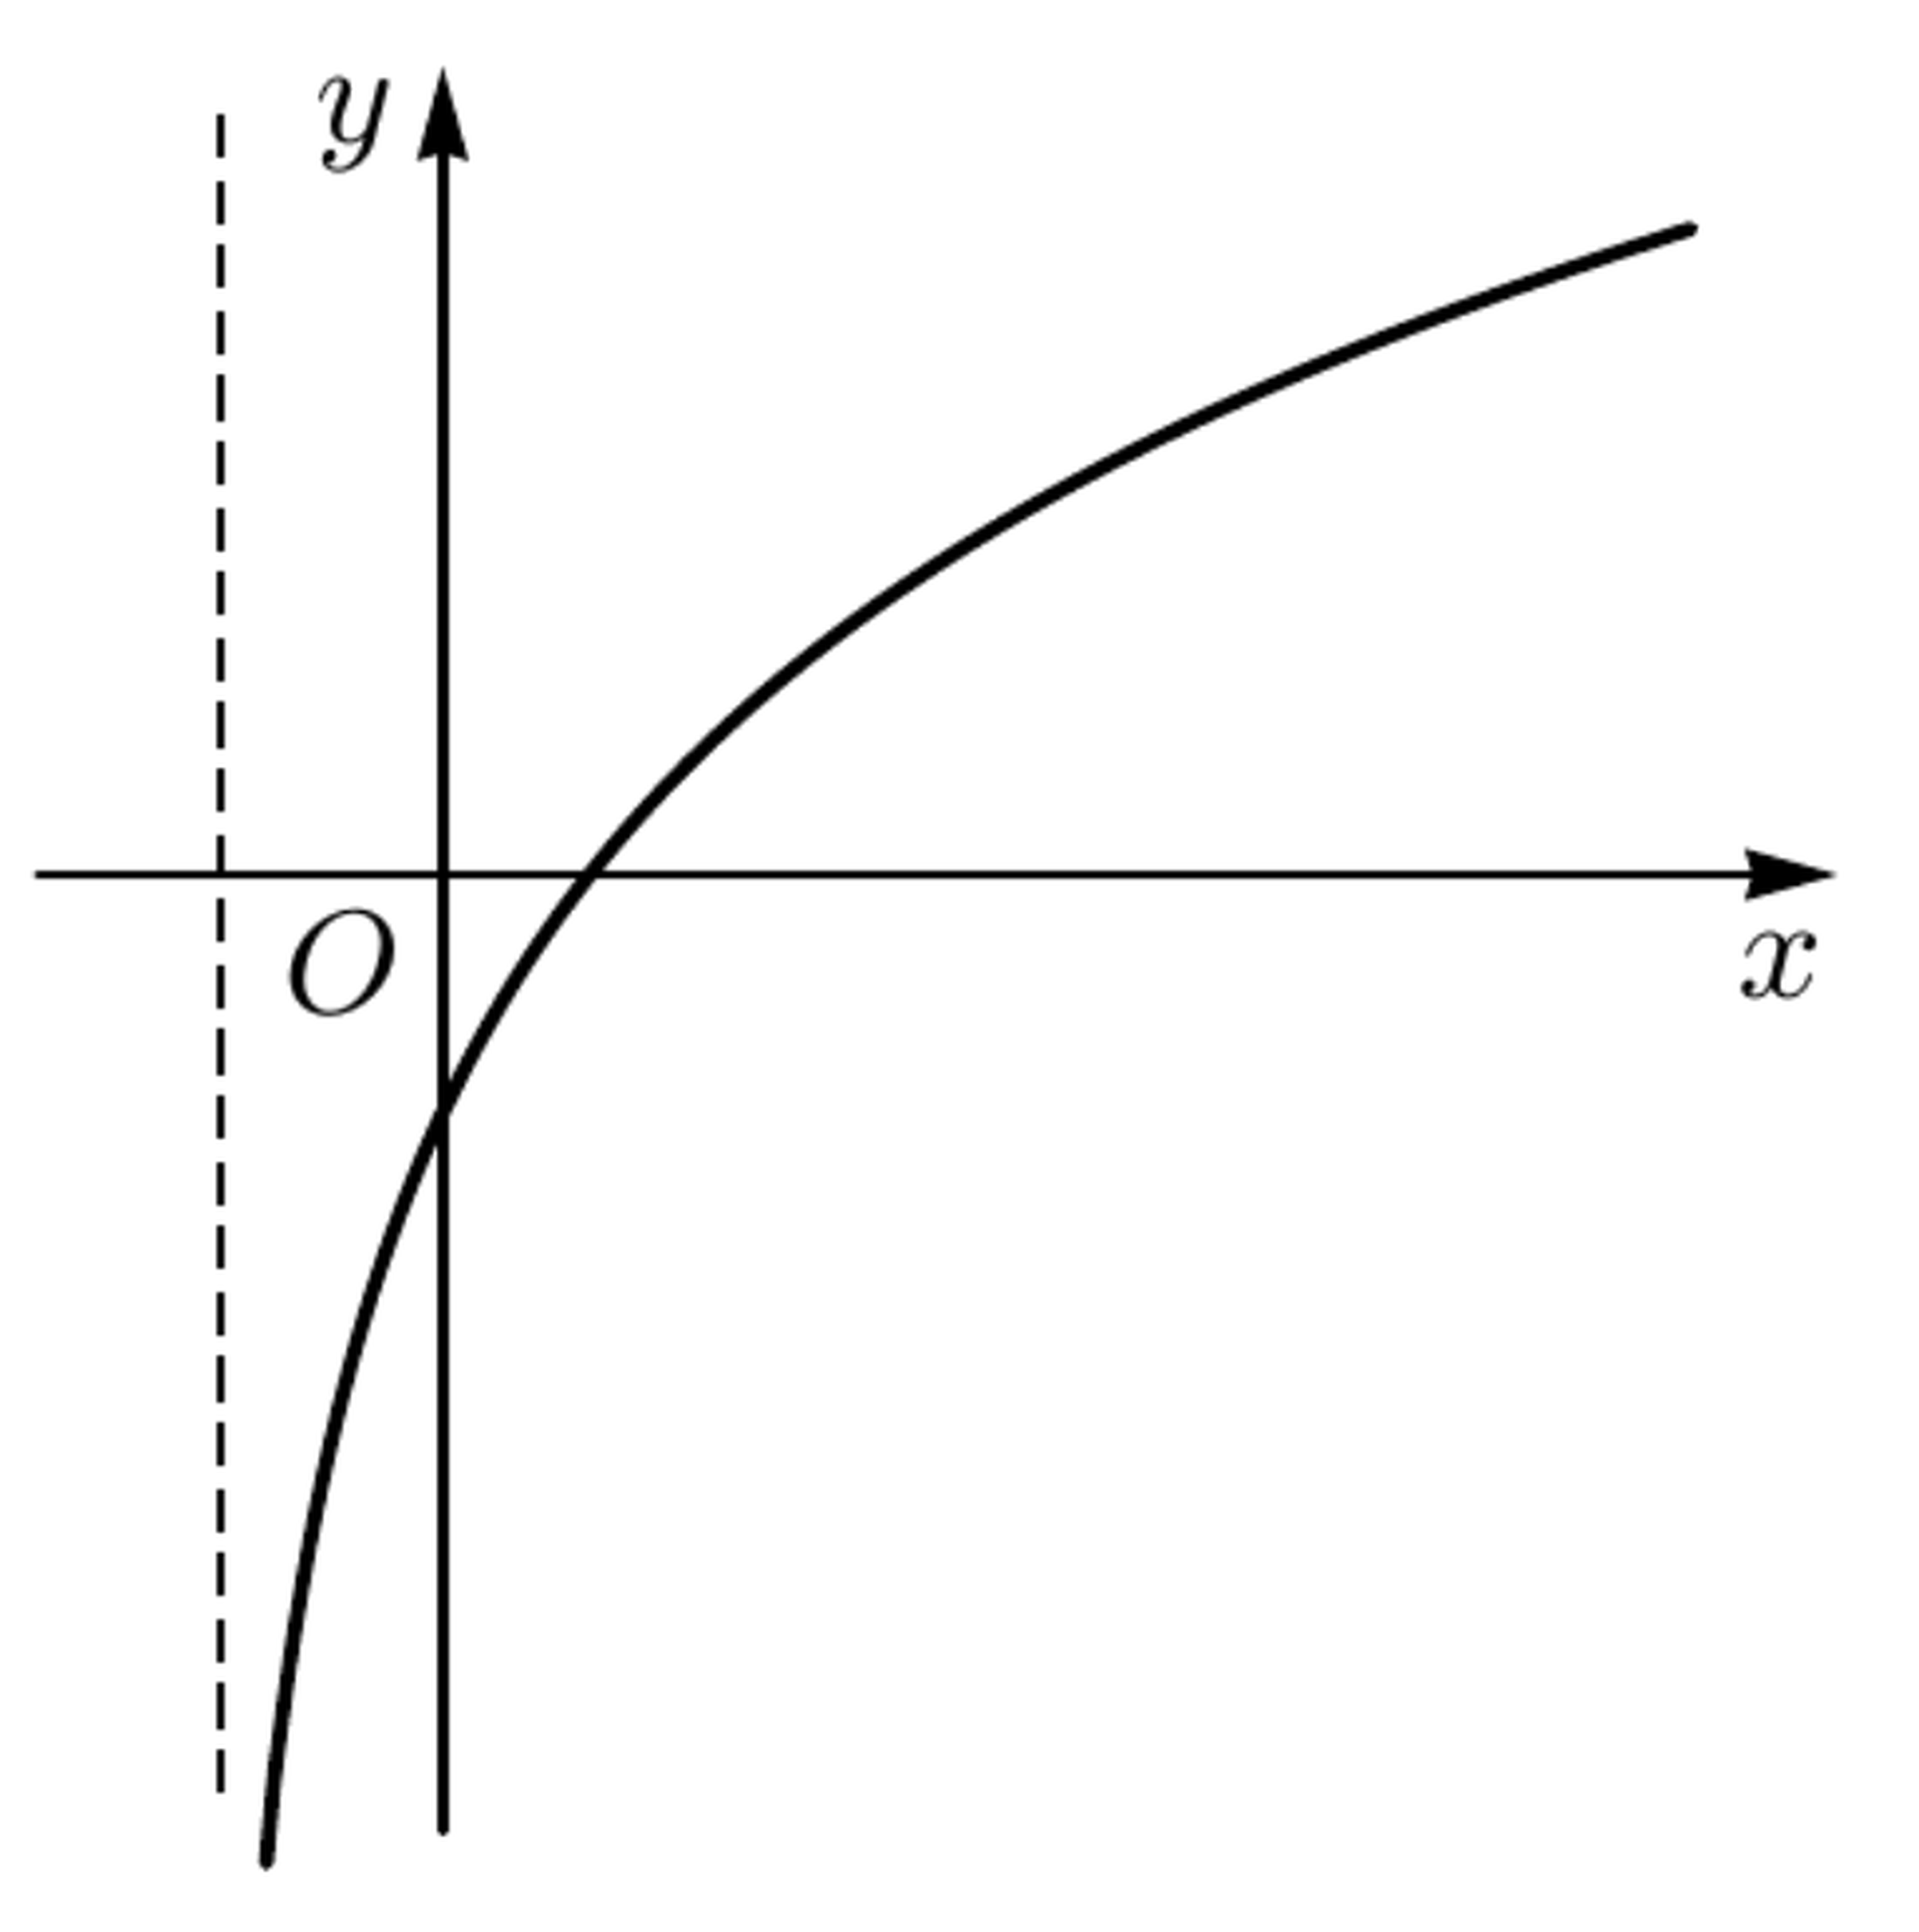
\includegraphics[width=0.42\textwidth]{figures/gao158_q15.png}
\end{center}

\keepwithprev
A. $a>1, b>1$\qquad\qquad B. $a>1, 0<b<1$

C. $0<a<1, b>1$\qquad\qquad D. $0<a<1, 0<b<1$

\ifanswer
\solbegin
\step{图像严格增，得 $a>1$.}
\step{图像与 $y$ 轴交于 $x$ 轴下方，得 $b>0$ 且 $\log_a b<0$，即 $0<b<1$，故选 $B$.}
\solend
\fi

% === Q16 === \lvert\log_2 x\rvert；解析 5 行，故选 C
\item 已知函数 $f(x)=\lvert\log_2 x\rvert$，若 $0<a<b$ 且 $f(a)=f(b)$，则 $a+2b$ 的取值范围是\mbox{（\quad）}

\keepwithprev
A. $(2\sqrt2,+\infty)$\qquad B. $[2\sqrt2,+\infty)$\qquad C. $(3,+\infty)$\qquad D. $[3,+\infty)$

\ifanswer
\solbegin
\step{由 $a<b$ 及 $\lvert\log_2 a\rvert=\lvert\log_2 b\rvert$，得 $\log_2 a=-\log_2 b$，即 $ab=1$，}
\step{且 $0<a<1<b$.}
\step{设 $t=a+2b=2b+\dfrac1b$，则 $t-3=\dfrac{(b-1)(2b-1)}{b}>0$.}
\step{反之，任取 $t>3$，令 $b=\dfrac{t+\sqrt{t^2-8}}{4}>1$、$a=\dfrac1b$，则满足题设且 $a+2b=t$.}
\step{因此取值范围为 $(3,+\infty)$，故选 $C$.}
\solend
\fi

\end{enumerate}

\bigsec{三、解答题}

\begin{enumerate}
\setcounter{enumi}{16}

% === Q17 === 集合、\overline{A}、\subseteq；解析 9 行
\item 已知全集 $U=\R$，集合 $A=\left\{x\mid\dfrac{x-3}{x+1}\leqslant0\right\}$，$B=\{x\mid x^2-2mx+m^2-9<0\}$（$m$ 为实数）.

(1) 当 $m=4$ 时，求 $A\cap B$ 和 $\overline{A}\cup B$；

(2) 若“$x\in A$”是“$x\in B$”的充分条件，求实数 $m$ 的取值范围.

\ifanswer
\solbegin
\step{(1) $\dfrac{x-3}{x+1}\leqslant0\Leftrightarrow-1<x\leqslant3$，所以 $A=(-1,3]$.}
\step{当 $m=4$ 时，$B=\{x\mid(x-4)^2<9\}=(1,7)$，}
\step{于是 $A\cap B=(1,3]$，$\overline{A}\cup B=(-\infty,-1]\cup(1,+\infty)$；}
\step{(2) $x^2-2mx+m^2-9<0\Leftrightarrow(x-m)^2<9$，所以 $B=(m-3,m+3)$.}
\step{题设充分条件等价于 $A\subseteq B$.}
\step{由于 $A=(-1,3]$，左端须满足 $m-3\leqslant-1$.}
\step{又 $3\in A$，须有 $3<m+3$.}
\step{这两个条件也保证 $(-1,3]\subseteq(m-3,m+3)$，}
\step{因此 $A\subseteq B\Leftrightarrow\begin{cases}m-3\leqslant-1\\m+3>3\end{cases}\Leftrightarrow0<m\leqslant2$.}
\solend
\fi

% === Q18 === 蓄水池造价（含 (3) 场地限制）；单位 \mathrm{m}；解析 13 行
\item 某工厂拟建一个容积为 $400\mathrm{m}^3$ 的无盖长方体蓄水池，池深 $4\mathrm{m}$，池底为矩形，其一边长
为 $x\mathrm{m}$. 池壁每平方米造价 100 元，池底每平方米造价 150 元. 设水池的总造价为 $C$
元.

(1) 把 $C$ 表示成 $x$ 的函数，并写出它的定义域；

(2) 当 $x$ 为何值时，总造价最低？最低造价是多少？

(3) 受场地限制，池底一边长 $x$ 不超过 $8\mathrm{m}$，此时总造价最低是多少？

\ifanswer
\solbegin
\step{(1) 设池底另一边长为 $y\mathrm{m}$，则 $4xy=400$，所以 $y=\dfrac{100}{x}$，$x>0$.}
\step{池底面积为 $100\mathrm{m}^2$，池壁总面积为 $8\left(x+\dfrac{100}{x}\right)\mathrm{m}^2$，}
\step{因此 $C(x)=100\times8\left(x+\dfrac{100}{x}\right)+150\times100=800x+\dfrac{80000}{x}+15000$，}
\step{定义域为 $(0,+\infty)$.}
\step{(2) 因为 $x>0$，所以 $C(x)=800\left(x+\dfrac{100}{x}\right)+15000$，}
\step{$\geqslant800\times2\sqrt{x\cdot\dfrac{100}{x}}+15000=31000$，}
\step{当且仅当 $x=\dfrac{100}{x}$，即 $x=10$ 时取等号.}
\step{答：当 $x=10$ 时，总造价最低，为 31000 元.}
\step{(3) 此时定义域为 $(0,8]$. 任取 $0<x_1<x_2\leqslant8$，}
\step{则 $C(x_2)-C(x_1)=800(x_2-x_1)\left(1-\dfrac{100}{x_1x_2}\right)<0$，}
\step{所以 $C(x)$ 在 $(0,8]$ 上严格递减，$x=8$ 时总造价最低，}
\step{且 $C(8)=800\times8+\dfrac{80000}{8}+15000=31400$.}
\step{答：受场地限制时，最低总造价为 31400 元.}
\solend
\fi

% === Q19 === 甲乙滤材 0.8^n／0.7^n；解析 17 行
\item 某环保公司研发了两种新型滤材甲和乙：污水每经过一层甲滤材，污染物含量减少
20\%；每经过一层乙滤材，污染物含量减少 30\%. 每层甲滤材成本 3 万元，每层乙滤材
成本 4 万元. 设原污水中污染物含量为 1，要求处理后污染物含量低于原来的 5\%.

(1) 若只使用一种滤材，污水经过 $n$ 层后污染物含量为 $y$，分别写出使用甲、乙两种滤材
时 $y$ 关于 $n$ 的函数关系式（$n$ 为正整数）；

(2) 若只使用一种滤材，分别求甲、乙至少各需要多少层，并比较哪种滤材的总成本更
低；

(3) 若两种滤材可以混合使用（先后顺序不影响效果），设使用甲滤材 $m$ 层、乙滤材 $n$
层（$m$、$n$ 为非负整数），求满足要求的最低总成本，并指出此时 $m$、$n$ 的值.

\ifanswer
\solbegin
\step{(1) 甲：$y=0.8^n$；乙：$y=0.7^n$，其中 $n$ 为正整数.}
\step{(2) 两种滤材均须满足 $y<0.05$，且污染物含量随层数增加而严格减少.}
\step{$0.8^{14}\approx0.04398<0.05<0.05498\approx0.8^{13}$，}
\step{$0.7^9=0.040353607<0.05<0.05764801=0.7^8$，}
\step{甲至少需要 14 层，成本为 $3\times14=42$ 万元；}
\step{乙至少需要 9 层，成本为 $4\times9=36$ 万元.}
\step{因此，只使用一种滤材时，使用乙滤材的总成本更低.}
\step{(3) 设总成本为 $C$ 万元，则 $C=3m+4n,0.8^m\cdot0.7^n<0.05,m,n\in\{0,1,2,\cdots\}$，}
\step{若 $m\geqslant3$，将其中 3 层甲替换为 2 层乙，}
\step{因为 $0.7^2=0.49<0.512=0.8^3,2\times4<3\times3$，}
\step{替换后污染物含量更低，成本减少 1 万元，因此最低成本方案必有 $m\leqslant2$.}
\step{当 $m=0$ 时，由第（2）小题得至少需要 9 层乙，最低成本为 36 万元.}
\step{当 $m=1$ 或 $m=2$ 时，$0.8\cdot0.7^7>0.8^2\cdot0.7^7=0.052706752>0.05$，}
\step{$0.8^2\cdot0.7^8<0.8\cdot0.7^8=0.046118408<0.05$，}
\step{因此两种情形均至少需要 8 层乙，}
\step{对应最低成本分别为 $3+4\times8=35$ 万元，$3\times2+4\times8=38$ 万元.}
\step{答：满足要求的最低总成本为 35 万元，此时使用甲滤材 1 层、乙滤材 8 层.}
\solend
\fi

% === Q20 === f(x)=\log_2(4^x+1)-x；\Delta；解析 17 行
\item 已知函数 $f(x)=\log_2(4^x+1)-x$.

(1) 证明 $f(x)=\log_2(2^x+2^{-x})$，并求 $f(x)$ 的最小值及取得最小值时 $x$ 的值；

(2) 解不等式 $f(x)>\log_2 5-1$；

(3) 证明：函数 $f(x)$ 在区间 $[0,+\infty)$ 上是严格增函数；并求使关于 $x$ 的方程 $f(x)=m$ 恰
有两个不同实数解的实数 $m$ 的取值范围.

\ifanswer
\solbegin
\step{(1) $f(x)=\log_2(4^x+1)-\log_2 2^x=\log_2\dfrac{4^x+1}{2^x}=\log_2(2^x+2^{-x})$，}
\step{因为 $2^x+2^{-x}\geqslant2\sqrt{2^x\cdot2^{-x}}=2$，所以 $f(x)\geqslant\log_2 2=1$，}
\step{等号当且仅当 $2^x=2^{-x}$，即 $x=0$ 时成立，故最小值为 1.}
\step{(2) 令 $t=2^x>0$，则 $f(x)>\log_2 5-1\Leftrightarrow t+\dfrac1t>\dfrac52\Leftrightarrow2t^2-5t+2>0$}
\step{$\Leftrightarrow(2t-1)(t-2)>0$，}
\step{结合 $t>0$，得 $0<t<\dfrac12$ 或 $t>2$，即 $x<-1$ 或 $x>1$，}
\step{解集为 $(-\infty,-1)\cup(1,+\infty)$.}
\step{(3) 任取 $0\leqslant x_1<x_2$，记 $a=2^{x_1}$，$b=2^{x_2}$，则 $1\leqslant a<b$，$ab>1$，}
\step{从而 $\left(b+\dfrac1b\right)-\left(a+\dfrac1a\right)=(b-a)\left(1-\dfrac{1}{ab}\right)>0$，}
\step{由对数函数的严格递增性，得 $f(x_1)<f(x_2)$，}
\step{所以 $f(x)$ 在 $[0,+\infty)$ 上是严格增函数.}
\step{当 $m<1$ 时，由（1）得方程无实数解；当 $m=1$ 时，只有实数解 $x=0$.}
\step{当 $m>1$ 时，令 $t=2^x>0$，则 $f(x)=m\Leftrightarrow t+\dfrac1t=2^m\Leftrightarrow t^2-2^m t+1=0$，}
\step{此时 $\Delta=2^{2m}-4>0$，两根之和为 $2^m>0$、之积为 $1>0$，}
\step{故有两个不同的正根.}
\step{每个正根 $t$ 唯一确定一个实数 $x=\log_2 t$，故原方程恰有两个不同实数解，}
\step{所求范围为 $m\in(1,+\infty)$.}
\solend
\fi

% === Q21 === f(x)=4^x-m\cdot2^{x+1}+3 值域与 h(m) 分段；解析 13 行
\item 已知函数 $f(x)=4^x-m\cdot2^{x+1}+3$（$m\in\R$），$x\in[0,2]$.

(1) 当 $m=1$ 时，求 $f(x)$ 的值域；

(2) 记 $f(x)$ 的最小值为 $h(m)$，求 $h(m)$ 的表达式；

(3) 若关于 $x$ 的方程 $f(x)=0$ 在区间 $[0,2]$ 上有解，求实数 $m$ 的取值范围.

\ifanswer
\solbegin
\step{令 $t=2^x$，则 $t\in[1,4]$，且 $f(x)=t^2-2mt+3=(t-m)^2+3-m^2$，}
\step{(1) 当 $m=1$ 时，$f(x)=(t-1)^2+2$.}
\step{由 $0\leqslant t-1\leqslant3$，得 $2\leqslant f(x)\leqslant11$，值域为 $[2,11]$.}
\step{(2) 二次函数 $y=(t-m)^2+3-m^2$ 的对称轴为直线 $t=m$.}
\step{当 $m\leqslant1$ 时，在 $t=1$ 处取最小值；}
\step{当 $1<m<4$ 时，在 $t=m$ 处取最小值；}
\step{当 $m\geqslant4$ 时，在 $t=4$ 处取最小值；}
\step{因此 $h(m)=\begin{cases}4-2m,&m\leqslant1\\3-m^2,&1<m<4\\19-8m,&m\geqslant4\end{cases}$；}
\step{(3) 方程 $f(x)=0$ 在 $[0,2]$ 上有解，}
\step{等价于存在 $t\in[1,4]$，使 $m=\dfrac{t^2+3}{2t}=\dfrac12\left(t+\dfrac3t\right)$，}
\step{由基本不等式，$m\geqslant\dfrac12\cdot2\sqrt{t\cdot\dfrac3t}=\sqrt3$，当且仅当 $t=\sqrt3$ 时取等号；}
\step{又 $\dfrac{19}{8}-m=\dfrac{(4-t)(4t-3)}{8t}\geqslant0$，当且仅当 $t=4$ 时取等号；}
\step{因此必有 $\sqrt3\leqslant m\leqslant\dfrac{19}{8}$.}
\solend
\fi

\end{enumerate}

\end{document}
"
% 紧凑版：xelatex "\def\iscompact{1}% 高一158_上实东滩_期中.tex
%   —— 高一上数学"2026-2027 年上实东滩高一上期中"（试卷版/答案版/紧凑版）
% 试卷版：xelatex 高一158_上实东滩_期中.tex
% 答案版：xelatex "\def\isanswer{1}\input{高一158_上实东滩_期中.tex}"
% 紧凑版：xelatex "\def\iscompact{1}\input{高一158_上实东滩_期中.tex}"
%
% ① 原始材料：微信公众号"魔都数学加油站"文章，连载"27学年高一158"，原文标题
% "27学年高一158——2026-2027年上海市上实东滩高一上期中"（本卷本地编号 158 与
% 原卷连载号一致，无撞号）。
% 正文为 9 张 PNG 页（01/05/08/09 为 2560×3620，02/03/04/06/07 为 4762×6735，
% 同一篇各页分辨率混排，逐页按各自分辨率裁图核对）。
% 体例：讲评版——填空 3—12（10 题）、选择 13—16（4 题）、解答 17—21（5 题），
% 共 19 题，自第 3 题起编（1、2 未印在本篇）；Q5 只印【答案】、其余 18 题
% 逐题印【解析】（逐题核实，见 ②）。题目、答案、解析均据原图转录；卷面粉红色
% 水印"魔都数学加油站"及公众号页脚未录入。全卷末题为第 21 题，无附加题节。
% 全卷 2 组配图（逐页通读 9 页确认）——
%   · Q10 题干右侧"曼 → man"字形变换图（02 页），题目配图、三版都出，
%     裁 figures/gao158_q10.png；
%   · Q15 题干"如图所示"对数函数大致图像（03 页右下），题目配图、三版都出，
%     裁 figures/gao158_q15.png；
% 2 图均取自原卷截图，去粉色水印、转灰度、4× LANCZOS 放大；
% 其余各页逐页确认无其它题目配图、无解析内配图、无表格。
%
% 卷首标题：原卷印作"2026-2027 年上实东滩高一上期中"，年份区间按全稿惯例排 en dash；
% 原卷卷面未印副标题，本稿按同期中卷知识模块口径补出"集合与常用逻辑用语、不等式、函数"。
%
% ② 与原卷的排版差异／照录项清单：
%   ① 原文从第 3 题起，本稿保留原题号；共 19 题三节，解答题 5 题到 21；
%      三节各自一个 enumerate＋各自 \setcounter{enumi}{2}／{12}／{16}，
%      不贯穿（题目溯源.py 按 \bigsec 切节、每节独立计 depth，只收 depth==1 的 \item）；
%   ② 混合体例：Q5 只印【答案】、无【解析】，按 高一156 第 3 题成例另提
%      \ans{}、不补造解析；其余 18 题印【解析】、用 \solbegin…\solend；
%      四道选择题答案均在解析末句"故选 C／B／B／C"（逐个放大复核）、
%      题干括号 \mbox{（\quad）} 留空、不另提 \ans{}；答案版
%      【答案】/【解析】标记数 = 19 = 全卷题数（1 个 \ans ＋ 18 个 \solbegin）；
%   ③ 原卷卷面未印副标题，本稿按知识模块口径补出；
%   ④ 原卷填空横线按全稿惯例排 \blankline[4.4em]；选择题选项段前按惯例各加
%      \keepwithprev；解答题不留作答区、不加 \anspace（原卷为讲评版）；
%   ⑤ 数集：Q13"在 \R 上严格递增"、Q14"$x\in\R$"、Q17"$U=\R$"、
%      Q21"$m\in\R$" 原卷印正体粗体 R，按全稿惯例归一 \R；
%      绝对值排 \lvert…\rvert（Q12 $\lvert a\rvert$、Q14 $\lvert x-2\rvert$、
%      Q16 $\lvert\log_2 x\rvert$／$\lvert\log_2 a\rvert$／$\lvert\log_2 b\rvert$），
%      集合描述竖线排 \mid（Q17），不等号按全稿惯例排 \leqslant／\geqslant，
%      补集上划线 \overline{A}（Q17）；
%   ⑥ 子集／真子集符号逐处照录不统一：Q14 解析"$(2,3)\subsetneq(1,3)$"原卷印
%      带下划线且被斜杠划过的 ⊊（真子集，放大 03 页确认），照录 \subsetneq；
%      Q17 解析三处"$A\subseteq B$""$(-1,3]\subseteq(m-3,m+3)$"原卷印
%      带下划线 ⊆（放大 05 页确认），照录 \subseteq；本卷无单线 \subset 用例；
%   ⑦ 判别式：Q20 (3) 解析"$\Delta=2^{2m}-4>0$"原卷印高瘦等腰 \Delta
%      （像素实测高/宽 ≈ 1.13，扁三角 \triangle 为 0.93，放大 08 页确认），
%      照录 \Delta；本卷无扁三角 \triangle 用例；
%   ⑧ "图像"与"图象"：全卷统一用"图像"（Q6 题干、Q10 两处、Q11 解析、
%      Q15 题干与解析两处，逐处放大确认带单人旁），照录不改；
%   ⑨ 中文弯引号照录：Q5 命题"若实数…"、Q10"曼""man""新"、Q14 题干与
%      解析的两则不等式、Q17 (2)"$x\in A$""$x\in B$"；注释里一律 ASCII 引号；
%   ⑩ 半角逗号逐处照录：Q8"$2,3,4$""$-2,-1,0$"、Q10 点坐标 $(x,y)$／
%      $(t,2^t-1)$／$(1-2^t,t)$、Q15 四选项"$a>1, b>1$"等、
%      Q19 (3)"$C=3m+4n,0.8^m\cdot0.7^n<0.05,m,n\in\{0,1,2,\cdots\}$"
%      与"$0.7^2=0.49<0.512=0.8^3,2\times4<3\times3$"、
%      Q21 cases 内"$4-2m,$"等；其余行中逗号／顿号照录全角；
%      行末西文句点 ASCII `.`；
%   ⑪ 顿号照录：Q3"（用 $a$、$b$ 表示）"、Q5"$x$、$y$"、Q13"A、B"、
%      Q16 解析"$>1$、$a=\dfrac1b$"、Q19"甲、乙""$m$、$n$"、
%      Q20"$2^m>0$、之积为"、Q21"$m$、$n$"；顿号一律移到数学模式外，
%      数学模式内不出现中文标点；
%   ⑫ 角度与单位照录：Q10 三处"$90^{\circ}$"、Q18"$400\mathrm{m}^3$"
%      "$4\mathrm{m}$""$x\mathrm{m}$""$8\mathrm{m}$""$y\mathrm{m}$"
%      "$100\mathrm{m}^2$""$\left(x+\dfrac{100}{x}\right)\mathrm{m}^2$"；
%      Q19 百分号"20\%""30\%""5\%"按原卷排 \%；
%   ⑬ 文本模式全角括号照录：Q10"（提示：…）"、Q17"（$m$ 为实数）"、
%      Q19"（$n$ 为正整数）""（先后顺序不影响效果）""（$m$、$n$ 为非负整数）"、
%      Q20"由（1）得"、Q19"由第（2）小题"、Q21"（$m\in\R$）"；
%      子题行首标号按全稿惯例用半角 (1)(2)(3)；
%   ⑭ 复杂式照录别简化：Q3 $\dfrac{\log_3 2+\log_3 5}{\log_3 3+2\log_3 2}$、
%      Q8 $[-3,-2)\cup(4,5]$、Q9 $18ab=2^t\cdot3^t=6^t=a+b$、
%      Q12 $\dfrac{\sqrt6}{2}$、Q18 $C(8)=800\times8+\dfrac{80000}{8}+15000=31400$
%      （原卷即 C(8)，非 C(2)）、Q19 $0.8^{14}\approx0.04398$、
%      $0.7^9=0.040353607$、$0.052706752$、$0.046118408$、
%      Q20 $t^2-2^m t+1=0$、Q21 $h(m)$ 三段 cases 与 $\dfrac{(4-t)(4t-3)}{8t}$ 等；
%      \left…\right 不得拆到不同 $…$ 组；cases 块整体算一个印刷行；
%   ⑮ 一条 \step = 原卷解析的一个印刷行；别并折行、别拆行。跨页续印按题合并
%      （Q7 的 01—02 页、Q9/Q10/Q11 的 02—03 页、Q13/Q14 的 03 页上下、
%      Q15/Q16 的 04 页上下、Q17 的 04—05 页、Q18 的 05—06 页、
%      Q19 的 06—07 页、Q20 的 07—08 页、Q21 的 08—09 页）；
%      跨半页重叠行（Q5【答案】、Q9 设公共值行、Q10 题干、Q16 反之行、
%      Q18 (2) 题干、Q19 末两行、Q20 (3) 末行、Q21 cases 块）只算一个印刷行；
%   ⑯ 配图：2 组题目配图（见 ①），均三版都出，\needvspace 守卫放 \item 之前
%      把"题干＋图"整块推走，\includegraphics 放题干之后；本卷无解析内配图、
%      无红字加粗小标题（全卷逐页确认，故无 \stepm）。
%
% ③ 行数复核：一条 \step = 原卷解析的一个印刷行，cases 块作一个印刷行计。
%   逐题数（逐页核对）：Q3：1；Q4：2；Q5：0（只印【答案】、提 \ans{}，
%   不计入 \step 账）；Q6：1；Q7：4；Q8：5；Q9：2；Q10：2；Q11：3；
%   Q12：3；Q13：2；Q14：3；Q15：2；Q16：5；Q17：9；Q18：13；
%   Q19：17；Q20：17；Q21：13。
%   合计 104 行（104 条 \step ＋ 0 条 \stepm），与原卷逐题印刷行相等。
%   全卷 19 题：Q5 一处 \ans{} ＋ 其余 18 题设 \solbegin…\solend，
%   答案版【答案】/【解析】标记数 = 19 = 全卷题数。
%
% ④ 页码分布（供回原图复核）：
%   卷首标题＋"一、填空题"＋Q3 题干＋解析 1 行、Q4 题干＋解析 2 行、
%   Q5 题干＋【答案】在 01 页上半；Q5【答案】（重叠重印）＋Q6 题干＋解析 1 行、
%   Q7 题干＋解析前 3 行在 01 页下半；Q7 解析末行＋Q8 题干＋解析 5 行、
%   Q9 题干＋解析首行在 02 页上半；Q9 解析末行＋Q10 题干（含"曼→man"图）
%   ＋解析 2 行＋Q11 题干＋解析首行在 02 页下半；Q11 解析后 2 行＋Q12 题干
%   ＋解析 3 行＋"二、选择题"标题＋Q13 题干＋选项在 03 页上半；
%   Q13 选项（重叠重印）＋解析 2 行＋Q14 题干＋选项＋解析 3 行＋Q15 题干
%   ＋对数图像（右侧）在 03 页下半；Q15 选项＋解析 2 行＋Q16 题干＋选项
%   ＋解析前 4 行在 04 页上半；Q16 解析末行＋"三、解答题"标题＋Q17 题干
%   ＋两问＋解析 (1) 3 行在 04 页下半；Q17 解析 (2) 6 行＋Q18 题干＋三问
%   ＋解析 (1) 4 行＋(2) 首行在 05 页上下；Q18 解析 (2) 后 3 行＋(3) 5 行
%   ＋Q19 题干＋三问＋解析 (1) 1 行＋(2) 3 行在 06 页上下；Q19 解析 (2) 3 行
%   ＋(3) 12 行在 07 页上半；Q19 解析末 2 行（重叠）＋Q20 题干＋三问
%   ＋解析 (1) 3 行在 07 页下半；Q20 解析 (2) 4 行＋(3) 前 4 行在 08 页上半；
%   Q20 解析 (3) 后 6 行＋Q21 题干＋(1) 问在 08 页下半；Q21 (2)(3) 问＋
%   解析 (1) 3 行＋(2) 5 行＋cases 块在 09 页上半；Q21 cases 块（重叠）
%   ＋(3) 解析 5 行在 09 页下半。本稿按题连排，不丢行、不并折行；
%   全卷末题为第 21 题，无附加题节。
%
% ⑤ 存疑／需主会话回原图复核：
%   1. Q14 解析"$(2,3)\subsetneq(1,3)$"的 ⊊（真子集带斜杠）与 Q17 的 ⊆
%      是两种不同记号，本稿分别照录 \subsetneq／\subseteq，请复核；
%   2. Q20 (3)"$\Delta=2^{2m}-4>0$"判为高瘦 \Delta，请复核是否 \triangle；
%   3. 任务书提示"Q18 解析里印 C(2)=…"，但 06 页原图逐处读作
%      $C(8)=800\times8+\dfrac{80000}{8}+15000=31400$，未找到 C(2)，
%      本稿照原卷排 C(8)，请复核；
%   4. Q19 解析末句"最低总成本为 35 万元"（07 页上下两处印同），
%      OCR 曾误读为 34，本稿按 35 照录，请复核；
%   5. Q10 提示末尾"坐标为 $(-y,x)$）."为半角 $)$＋全角 $）$ 两枚括号，
%      本稿照录，请复核；
%   6. Q21 cases 块后"；"落在分式中行右侧（排版居中基线所致），
%      本稿排作 $…\end{cases}$；，请复核。
%   全卷除此 6 类外未发现其它笔误／自相矛盾处；19 题中 18 题印【解析】。
%
\documentclass[a4paper,11pt]{article}
\usepackage{common}

\begin{document}

\examtitlest[3]{2026--2027 年上实东滩高一上期中}{集合与常用逻辑用语、不等式、函数}

\bigsec{一、填空题}

\begin{enumerate}
\setcounter{enumi}{2}

% === Q3 === 换底公式；解析 1 行
\item 已知 $3^a=5$，$\log_3 2=b$，则 $\log_{12} 10=$\blankline[4.4em]（用 $a$、$b$ 表示）.

\ifanswer
\solbegin
\step{$\log_{12} 10=\dfrac{\log_3 2+\log_3 5}{\log_3 3+2\log_3 2}=\dfrac{a+b}{1+2b}$.}
\solend
\fi

% === Q4 === 定义域；解析 2 行；半角括号 ( ) 与全角逗号照录
\item 函数 $y=\sqrt{2-x}+\lg(x^2-1)$ 的定义域为\blankline[4.4em].

\ifanswer
\solbegin
\step{由 $2-x\geqslant0$ 且 $x^2-1>0$，得 $x\leqslant2$ 且 ($x<-1$或$x>1$)，}
\step{定义域为 $(-\infty,-1)\cup(1,2]$.}
\solend
\fi

% === Q5 === 只印【答案】、无【解析】；反证法，中文弯引号
\item 用反证法证明命题“若实数 $x$、$y$ 满足 $x+y>2$，则 $x$、$y$ 中至少有一个大于 1”时，
应假设\blankline[4.4em].

\ifanswer
\ans{$x\leqslant1$ 且 $y\leqslant1$}
\fi

% === Q6 === 图像平移；解析 1 行
\item 函数 $y=\dfrac{2x+1}{x-1}$ 的图像可由函数 $y=\dfrac{3}{x}$ 的图像先向右平移 $a$ 个单位，再向上平移 $b$ 个单位
得到，则 $a+b=$\blankline[4.4em].

\ifanswer
\solbegin
\step{$y=\dfrac{2x+1}{x-1}=\dfrac{3}{x-1}+2$，所以 $a=1$，$b=2$，$a+b=3$.}
\solend
\fi

% === Q7 === 集合三元子集；解析 4 行，跨 01—02 页
\item 设 $A=\{a_1,a_2,a_3,a_4\}$ 是由四个实数组成的集合，若 $A$ 的所有三元子集中，三个元素之和
组成的集合为 $B=\{1,4,7,12\}$，则集合 $A=$\blankline[4.4em].

\ifanswer
\solbegin
\step{设 $S=a_1+a_2+a_3+a_4$，}
\step{每个元素在四个三元子集中恰出现三次，则 $3S=1+4+7+12=24$，得 $S=8$.}
\step{四个三元子集的元素和分别为 $S-a_i$，}
\step{所以 $A=\{8-1,8-4,8-7,8-12\}=\{-4,1,4,7\}$.}
\solend
\fi

% === Q8 === 不等式整数解；解析 5 行；半角逗号照录
\item 不等式 $x^2-(a+1)x+a<0$ 的解集中恰有 3 个整数，则 $a$ 的取值范围是\blankline[4.4em].

\ifanswer
\solbegin
\step{原不等式为 $(x-1)(x-a)<0$；}
\step{$a=1$ 时解集为空集，不符合题意.}
\step{若 $a>1$，解集为 $(1,a)$，恰含整数 $2,3,4$，则 $4<a\leqslant5$.}
\step{若 $a<1$，解集为 $(a,1)$，恰含整数 $-2,-1,0$，则 $-3\leqslant a<-2$.}
\step{故 $a$ 的取值范围是 $[-3,-2)\cup(4,5]$.}
\solend
\fi

% === Q9 === 对数换底＋指数；解析 2 行
\item 已知正数 $a$、$b$ 满足 $1+\log_2 a=2+\log_3 b=\log_6(a+b)$，则 $\dfrac1a+\dfrac1b=$\blankline[4.4em].

\ifanswer
\solbegin
\step{设公共值为 $t$，则 $2a=2^t$，$9b=3^t$，$a+b=6^t$，}
\step{于是 $18ab=2^t\cdot3^t=6^t=a+b$，即 $\dfrac1a+\dfrac1b=\dfrac{a+b}{ab}=18$.}
\solend
\fi

% === Q10 === "曼"字旋转 90°；题目配图（三版都出）；解析 2 行
\needvspace{6cm}
\item 网上流传一个有趣的字形变换：把汉字“曼”的右半部分旋转 $90^{\circ}$，就得到英文单词
“man”的艺术字. 数学中，把曲线绕原点旋转也会得到“新”的曲线：将函数
$y=2^x-1$ 的图像绕坐标原点 $O$ 逆时针旋转 $90^{\circ}$，得到的曲线恰是某个函数的
图像，则这个函数的解析式为\blankline[4.4em]（提示：点 $(x,y)$ 绕 $O$ 逆时针旋转 $90^{\circ}$ 后的
坐标为 $(-y,x)$）.

\begin{center}

\includegraphics[width=0.42\textwidth]{figures/gao158_q10.png}
\end{center}

\ifanswer
\solbegin
\step{原图像上的点 $(t,2^t-1)$ 旋转后为 $(1-2^t,t)$.}
\step{记其为 $(x,y)$，则 $x=1-2^y$，即 $y=\log_2(1-x)$，定义域为 $(-\infty,1)$.}
\solend
\fi

% === Q11 === 值域；解析 3 行，跨 02—03 页
\item 函数 $f(x)=\sqrt{x-2}-\sqrt{15-3x}$ 的值域为\blankline[4.4em].

\ifanswer
\solbegin
\step{由 $x-2\geqslant0$ 且 $15-3x\geqslant0$，得定义域为 $[2,5]$.}
\step{在 $[2,5]$ 上，$\sqrt{x-2}$ 与 $-\sqrt{15-3x}$ 均严格递增，因此 $f(x)$ 严格递增.}
\step{$f(2)=-3$，$f(5)=\sqrt3$，结合函数的图像，值域为 $[-3,\sqrt3]$.}
\solend
\fi

% === Q12 === 绝对值 \lvert…\rvert；解析 3 行
\item 设实数 $a$ 满足 $a<4a^3-5a<\lvert a\rvert$，则 $a$ 的取值范围是\blankline[4.4em].

\ifanswer
\solbegin
\step{由 $a<\lvert a\rvert$ 得 $a<0$，原不等式为 $a<4a^3-5a<-a$.}
\step{同除以 $a<0$，得 $1>4a^2-5>-1\Leftrightarrow1<a^2<\dfrac32$，结合 $a<0$，}
\step{得 $-\dfrac{\sqrt6}{2}<a<-1$，故解集为 $\left(-\dfrac{\sqrt6}{2},-1\right)$.}
\solend
\fi

\end{enumerate}

\bigsec{二、选择题}

\begin{enumerate}
\setcounter{enumi}{12}

% === Q13 === \R 归一；解析 2 行，故选 C
\item 已知 $a>b$，则下列不等式一定成立的是\mbox{（\quad）}

\keepwithprev
A. $\dfrac1a<\dfrac1b$\qquad B. $a^2>b^2$\qquad C. $a^3>b^3$\qquad D. $ac^2>bc^2$

\ifanswer
\solbegin
\step{幂函数 $y=x^3$ 在 $\R$ 上严格递增，$a>b\Rightarrow a^3>b^3$，C 正确.}
\step{取 $a=1$，$b=-1$ 得 A、B 不成立；取 $c=0$ 得 D 不成立；故选 $C$.}
\solend
\fi

% === Q14 === \subsetneq 真子集；解析 3 行，故选 B
\item 设 $x\in\R$，则“$\lvert x-2\rvert<1$”是“$x^2-5x+6<0$”的\mbox{（\quad）}

\keepwithprev
A. 充分非必要条件\qquad\qquad B. 必要非充分条件

C. 充要条件\qquad\qquad D. 既非充分又非必要条件

\ifanswer
\solbegin
\step{$\lvert x-2\rvert<1\Leftrightarrow1<x<3$，$x^2-5x+6<0\Leftrightarrow(x-2)(x-3)<0\Leftrightarrow2<x<3$.}
\step{由 $(2,3)\subsetneq(1,3)$，得“$\lvert x-2\rvert<1$”是“$x^2-5x+6<0$”的必要非充分条件，}
\step{故选 $B$.}
\solend
\fi

% === Q15 === 对数函数大致图像（题目配图，三版都出）；解析 2 行，故选 B
\needvspace{9cm}
\item 已知函数 $f(x)=\log_a(x+b)$（$a>0$ 且 $a\ne1$）的大致图像如图所示，则 $a$、$b$ 满足
的关系是\mbox{（\quad）}

\begin{center}
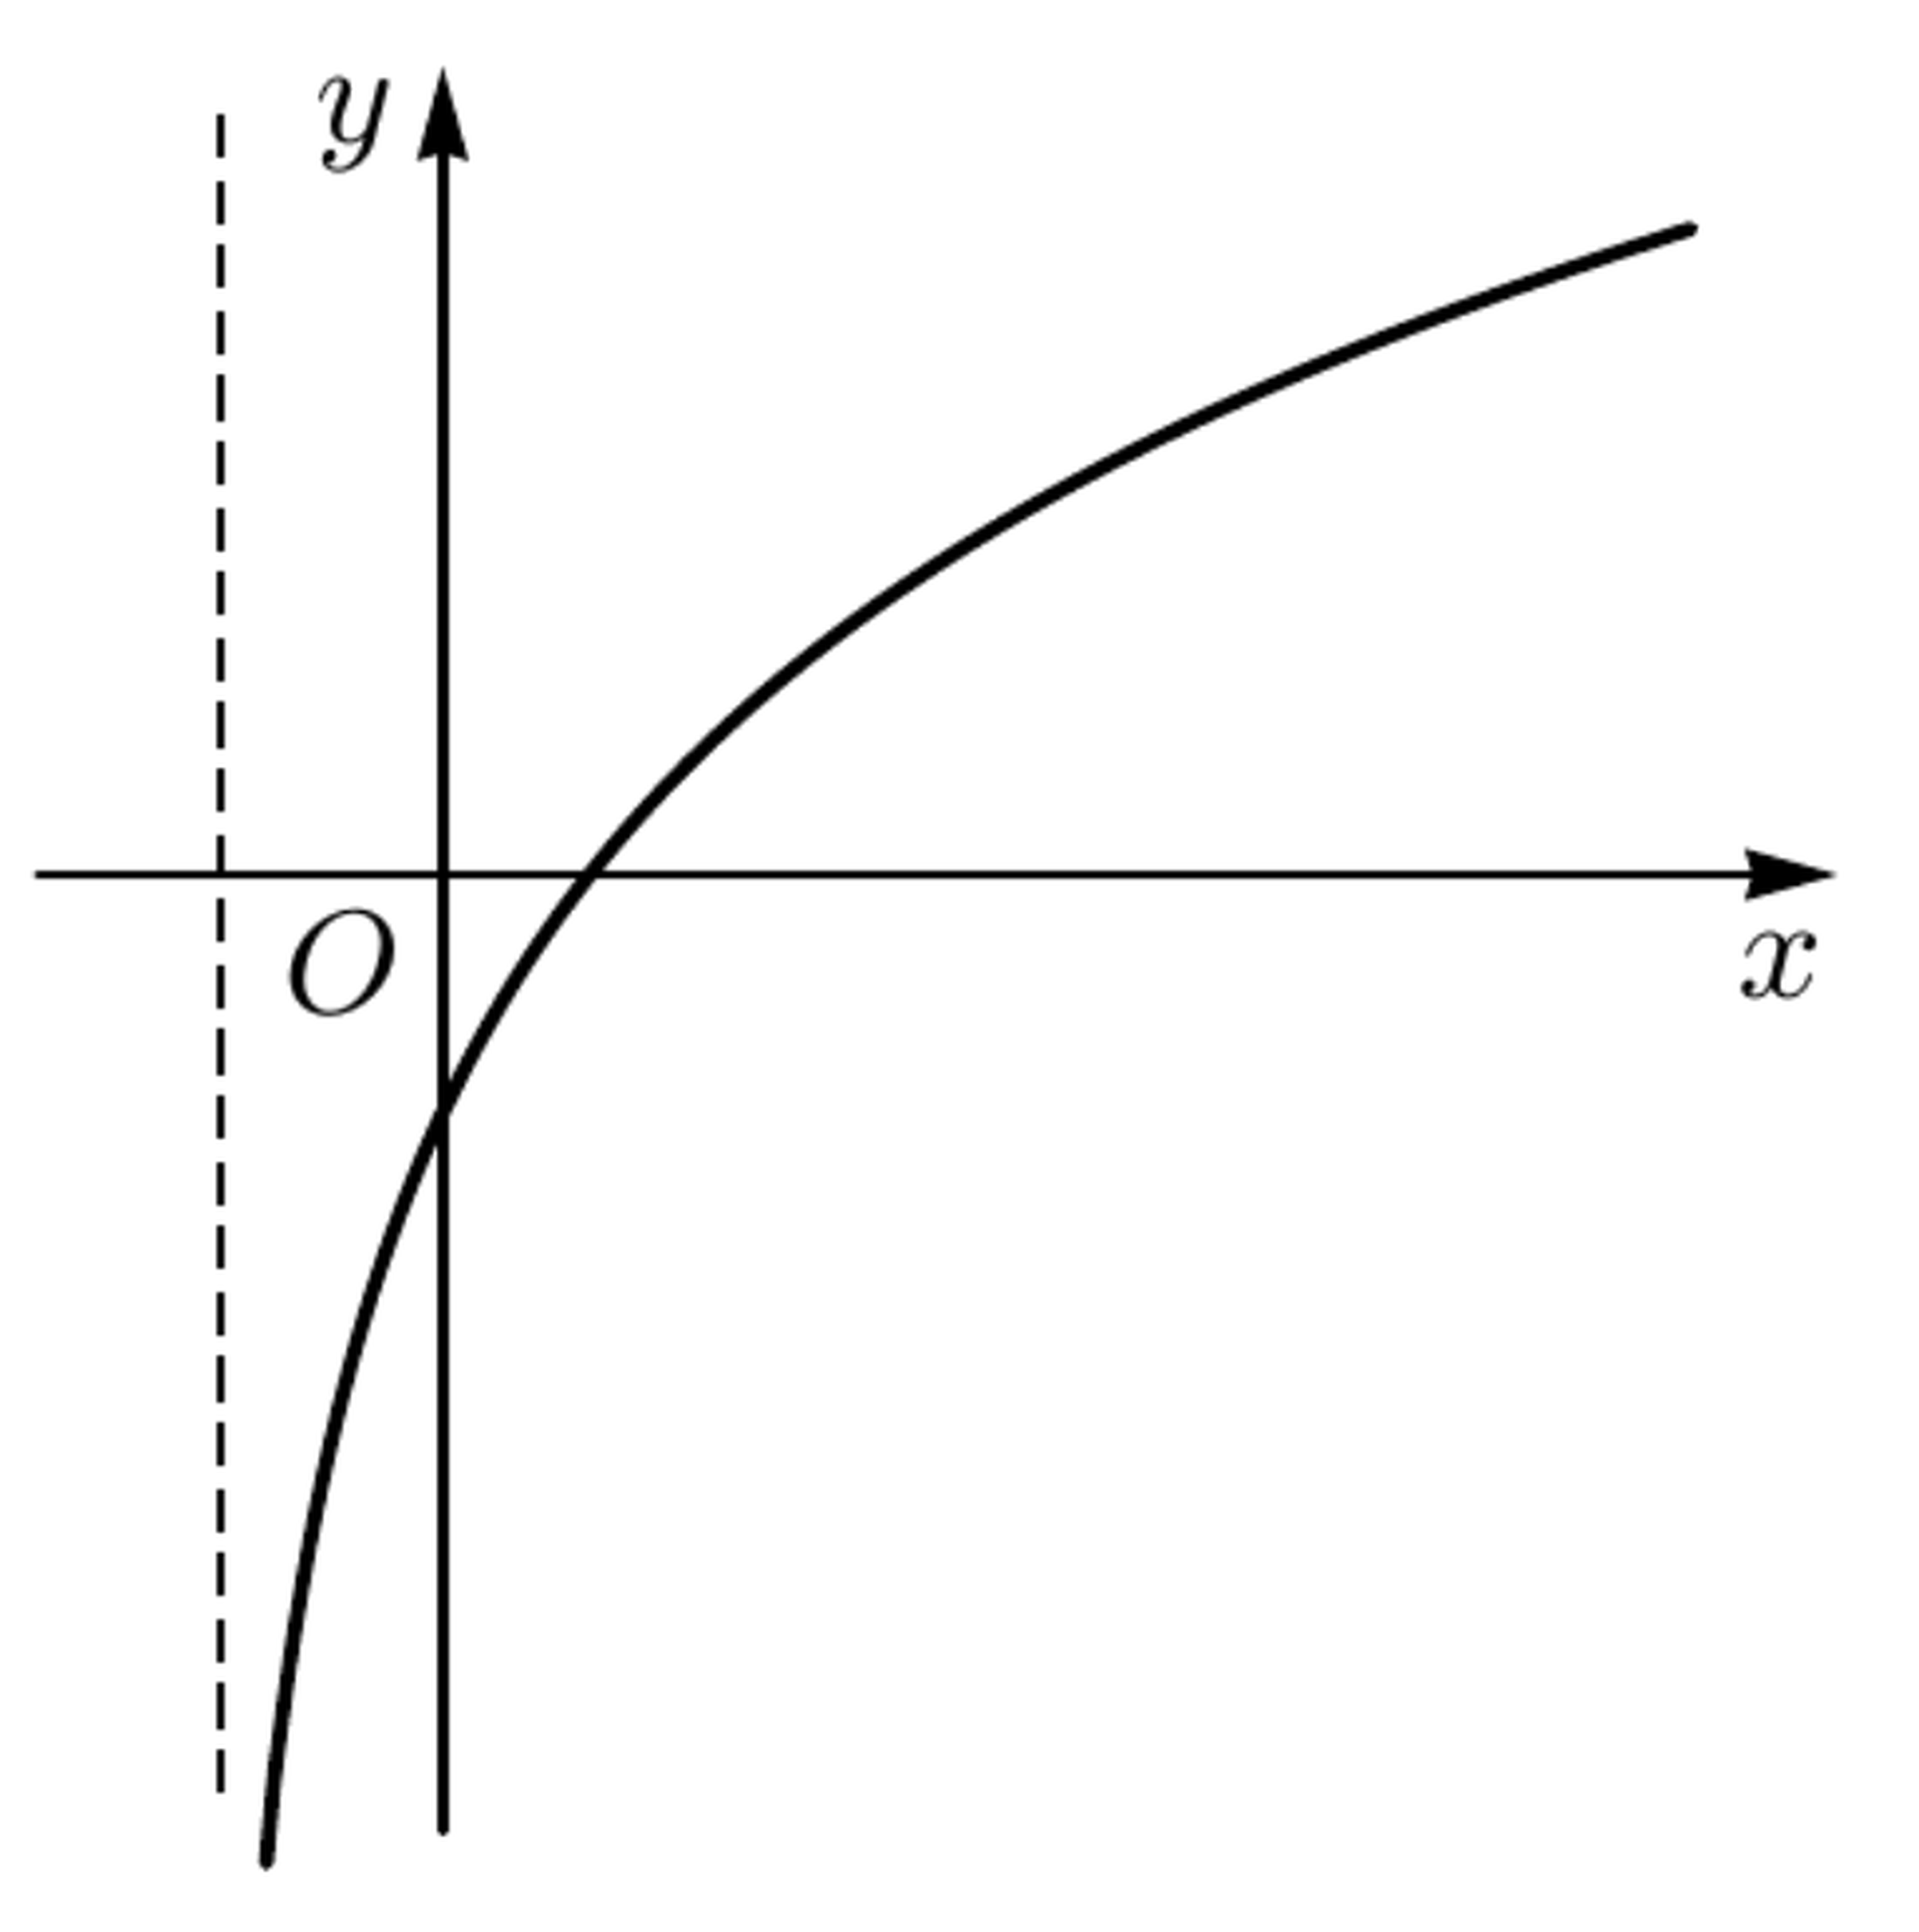
\includegraphics[width=0.42\textwidth]{figures/gao158_q15.png}
\end{center}

\keepwithprev
A. $a>1, b>1$\qquad\qquad B. $a>1, 0<b<1$

C. $0<a<1, b>1$\qquad\qquad D. $0<a<1, 0<b<1$

\ifanswer
\solbegin
\step{图像严格增，得 $a>1$.}
\step{图像与 $y$ 轴交于 $x$ 轴下方，得 $b>0$ 且 $\log_a b<0$，即 $0<b<1$，故选 $B$.}
\solend
\fi

% === Q16 === \lvert\log_2 x\rvert；解析 5 行，故选 C
\item 已知函数 $f(x)=\lvert\log_2 x\rvert$，若 $0<a<b$ 且 $f(a)=f(b)$，则 $a+2b$ 的取值范围是\mbox{（\quad）}

\keepwithprev
A. $(2\sqrt2,+\infty)$\qquad B. $[2\sqrt2,+\infty)$\qquad C. $(3,+\infty)$\qquad D. $[3,+\infty)$

\ifanswer
\solbegin
\step{由 $a<b$ 及 $\lvert\log_2 a\rvert=\lvert\log_2 b\rvert$，得 $\log_2 a=-\log_2 b$，即 $ab=1$，}
\step{且 $0<a<1<b$.}
\step{设 $t=a+2b=2b+\dfrac1b$，则 $t-3=\dfrac{(b-1)(2b-1)}{b}>0$.}
\step{反之，任取 $t>3$，令 $b=\dfrac{t+\sqrt{t^2-8}}{4}>1$、$a=\dfrac1b$，则满足题设且 $a+2b=t$.}
\step{因此取值范围为 $(3,+\infty)$，故选 $C$.}
\solend
\fi

\end{enumerate}

\bigsec{三、解答题}

\begin{enumerate}
\setcounter{enumi}{16}

% === Q17 === 集合、\overline{A}、\subseteq；解析 9 行
\item 已知全集 $U=\R$，集合 $A=\left\{x\mid\dfrac{x-3}{x+1}\leqslant0\right\}$，$B=\{x\mid x^2-2mx+m^2-9<0\}$（$m$ 为实数）.

(1) 当 $m=4$ 时，求 $A\cap B$ 和 $\overline{A}\cup B$；

(2) 若“$x\in A$”是“$x\in B$”的充分条件，求实数 $m$ 的取值范围.

\ifanswer
\solbegin
\step{(1) $\dfrac{x-3}{x+1}\leqslant0\Leftrightarrow-1<x\leqslant3$，所以 $A=(-1,3]$.}
\step{当 $m=4$ 时，$B=\{x\mid(x-4)^2<9\}=(1,7)$，}
\step{于是 $A\cap B=(1,3]$，$\overline{A}\cup B=(-\infty,-1]\cup(1,+\infty)$；}
\step{(2) $x^2-2mx+m^2-9<0\Leftrightarrow(x-m)^2<9$，所以 $B=(m-3,m+3)$.}
\step{题设充分条件等价于 $A\subseteq B$.}
\step{由于 $A=(-1,3]$，左端须满足 $m-3\leqslant-1$.}
\step{又 $3\in A$，须有 $3<m+3$.}
\step{这两个条件也保证 $(-1,3]\subseteq(m-3,m+3)$，}
\step{因此 $A\subseteq B\Leftrightarrow\begin{cases}m-3\leqslant-1\\m+3>3\end{cases}\Leftrightarrow0<m\leqslant2$.}
\solend
\fi

% === Q18 === 蓄水池造价（含 (3) 场地限制）；单位 \mathrm{m}；解析 13 行
\item 某工厂拟建一个容积为 $400\mathrm{m}^3$ 的无盖长方体蓄水池，池深 $4\mathrm{m}$，池底为矩形，其一边长
为 $x\mathrm{m}$. 池壁每平方米造价 100 元，池底每平方米造价 150 元. 设水池的总造价为 $C$
元.

(1) 把 $C$ 表示成 $x$ 的函数，并写出它的定义域；

(2) 当 $x$ 为何值时，总造价最低？最低造价是多少？

(3) 受场地限制，池底一边长 $x$ 不超过 $8\mathrm{m}$，此时总造价最低是多少？

\ifanswer
\solbegin
\step{(1) 设池底另一边长为 $y\mathrm{m}$，则 $4xy=400$，所以 $y=\dfrac{100}{x}$，$x>0$.}
\step{池底面积为 $100\mathrm{m}^2$，池壁总面积为 $8\left(x+\dfrac{100}{x}\right)\mathrm{m}^2$，}
\step{因此 $C(x)=100\times8\left(x+\dfrac{100}{x}\right)+150\times100=800x+\dfrac{80000}{x}+15000$，}
\step{定义域为 $(0,+\infty)$.}
\step{(2) 因为 $x>0$，所以 $C(x)=800\left(x+\dfrac{100}{x}\right)+15000$，}
\step{$\geqslant800\times2\sqrt{x\cdot\dfrac{100}{x}}+15000=31000$，}
\step{当且仅当 $x=\dfrac{100}{x}$，即 $x=10$ 时取等号.}
\step{答：当 $x=10$ 时，总造价最低，为 31000 元.}
\step{(3) 此时定义域为 $(0,8]$. 任取 $0<x_1<x_2\leqslant8$，}
\step{则 $C(x_2)-C(x_1)=800(x_2-x_1)\left(1-\dfrac{100}{x_1x_2}\right)<0$，}
\step{所以 $C(x)$ 在 $(0,8]$ 上严格递减，$x=8$ 时总造价最低，}
\step{且 $C(8)=800\times8+\dfrac{80000}{8}+15000=31400$.}
\step{答：受场地限制时，最低总造价为 31400 元.}
\solend
\fi

% === Q19 === 甲乙滤材 0.8^n／0.7^n；解析 17 行
\item 某环保公司研发了两种新型滤材甲和乙：污水每经过一层甲滤材，污染物含量减少
20\%；每经过一层乙滤材，污染物含量减少 30\%. 每层甲滤材成本 3 万元，每层乙滤材
成本 4 万元. 设原污水中污染物含量为 1，要求处理后污染物含量低于原来的 5\%.

(1) 若只使用一种滤材，污水经过 $n$ 层后污染物含量为 $y$，分别写出使用甲、乙两种滤材
时 $y$ 关于 $n$ 的函数关系式（$n$ 为正整数）；

(2) 若只使用一种滤材，分别求甲、乙至少各需要多少层，并比较哪种滤材的总成本更
低；

(3) 若两种滤材可以混合使用（先后顺序不影响效果），设使用甲滤材 $m$ 层、乙滤材 $n$
层（$m$、$n$ 为非负整数），求满足要求的最低总成本，并指出此时 $m$、$n$ 的值.

\ifanswer
\solbegin
\step{(1) 甲：$y=0.8^n$；乙：$y=0.7^n$，其中 $n$ 为正整数.}
\step{(2) 两种滤材均须满足 $y<0.05$，且污染物含量随层数增加而严格减少.}
\step{$0.8^{14}\approx0.04398<0.05<0.05498\approx0.8^{13}$，}
\step{$0.7^9=0.040353607<0.05<0.05764801=0.7^8$，}
\step{甲至少需要 14 层，成本为 $3\times14=42$ 万元；}
\step{乙至少需要 9 层，成本为 $4\times9=36$ 万元.}
\step{因此，只使用一种滤材时，使用乙滤材的总成本更低.}
\step{(3) 设总成本为 $C$ 万元，则 $C=3m+4n,0.8^m\cdot0.7^n<0.05,m,n\in\{0,1,2,\cdots\}$，}
\step{若 $m\geqslant3$，将其中 3 层甲替换为 2 层乙，}
\step{因为 $0.7^2=0.49<0.512=0.8^3,2\times4<3\times3$，}
\step{替换后污染物含量更低，成本减少 1 万元，因此最低成本方案必有 $m\leqslant2$.}
\step{当 $m=0$ 时，由第（2）小题得至少需要 9 层乙，最低成本为 36 万元.}
\step{当 $m=1$ 或 $m=2$ 时，$0.8\cdot0.7^7>0.8^2\cdot0.7^7=0.052706752>0.05$，}
\step{$0.8^2\cdot0.7^8<0.8\cdot0.7^8=0.046118408<0.05$，}
\step{因此两种情形均至少需要 8 层乙，}
\step{对应最低成本分别为 $3+4\times8=35$ 万元，$3\times2+4\times8=38$ 万元.}
\step{答：满足要求的最低总成本为 35 万元，此时使用甲滤材 1 层、乙滤材 8 层.}
\solend
\fi

% === Q20 === f(x)=\log_2(4^x+1)-x；\Delta；解析 17 行
\item 已知函数 $f(x)=\log_2(4^x+1)-x$.

(1) 证明 $f(x)=\log_2(2^x+2^{-x})$，并求 $f(x)$ 的最小值及取得最小值时 $x$ 的值；

(2) 解不等式 $f(x)>\log_2 5-1$；

(3) 证明：函数 $f(x)$ 在区间 $[0,+\infty)$ 上是严格增函数；并求使关于 $x$ 的方程 $f(x)=m$ 恰
有两个不同实数解的实数 $m$ 的取值范围.

\ifanswer
\solbegin
\step{(1) $f(x)=\log_2(4^x+1)-\log_2 2^x=\log_2\dfrac{4^x+1}{2^x}=\log_2(2^x+2^{-x})$，}
\step{因为 $2^x+2^{-x}\geqslant2\sqrt{2^x\cdot2^{-x}}=2$，所以 $f(x)\geqslant\log_2 2=1$，}
\step{等号当且仅当 $2^x=2^{-x}$，即 $x=0$ 时成立，故最小值为 1.}
\step{(2) 令 $t=2^x>0$，则 $f(x)>\log_2 5-1\Leftrightarrow t+\dfrac1t>\dfrac52\Leftrightarrow2t^2-5t+2>0$}
\step{$\Leftrightarrow(2t-1)(t-2)>0$，}
\step{结合 $t>0$，得 $0<t<\dfrac12$ 或 $t>2$，即 $x<-1$ 或 $x>1$，}
\step{解集为 $(-\infty,-1)\cup(1,+\infty)$.}
\step{(3) 任取 $0\leqslant x_1<x_2$，记 $a=2^{x_1}$，$b=2^{x_2}$，则 $1\leqslant a<b$，$ab>1$，}
\step{从而 $\left(b+\dfrac1b\right)-\left(a+\dfrac1a\right)=(b-a)\left(1-\dfrac{1}{ab}\right)>0$，}
\step{由对数函数的严格递增性，得 $f(x_1)<f(x_2)$，}
\step{所以 $f(x)$ 在 $[0,+\infty)$ 上是严格增函数.}
\step{当 $m<1$ 时，由（1）得方程无实数解；当 $m=1$ 时，只有实数解 $x=0$.}
\step{当 $m>1$ 时，令 $t=2^x>0$，则 $f(x)=m\Leftrightarrow t+\dfrac1t=2^m\Leftrightarrow t^2-2^m t+1=0$，}
\step{此时 $\Delta=2^{2m}-4>0$，两根之和为 $2^m>0$、之积为 $1>0$，}
\step{故有两个不同的正根.}
\step{每个正根 $t$ 唯一确定一个实数 $x=\log_2 t$，故原方程恰有两个不同实数解，}
\step{所求范围为 $m\in(1,+\infty)$.}
\solend
\fi

% === Q21 === f(x)=4^x-m\cdot2^{x+1}+3 值域与 h(m) 分段；解析 13 行
\item 已知函数 $f(x)=4^x-m\cdot2^{x+1}+3$（$m\in\R$），$x\in[0,2]$.

(1) 当 $m=1$ 时，求 $f(x)$ 的值域；

(2) 记 $f(x)$ 的最小值为 $h(m)$，求 $h(m)$ 的表达式；

(3) 若关于 $x$ 的方程 $f(x)=0$ 在区间 $[0,2]$ 上有解，求实数 $m$ 的取值范围.

\ifanswer
\solbegin
\step{令 $t=2^x$，则 $t\in[1,4]$，且 $f(x)=t^2-2mt+3=(t-m)^2+3-m^2$，}
\step{(1) 当 $m=1$ 时，$f(x)=(t-1)^2+2$.}
\step{由 $0\leqslant t-1\leqslant3$，得 $2\leqslant f(x)\leqslant11$，值域为 $[2,11]$.}
\step{(2) 二次函数 $y=(t-m)^2+3-m^2$ 的对称轴为直线 $t=m$.}
\step{当 $m\leqslant1$ 时，在 $t=1$ 处取最小值；}
\step{当 $1<m<4$ 时，在 $t=m$ 处取最小值；}
\step{当 $m\geqslant4$ 时，在 $t=4$ 处取最小值；}
\step{因此 $h(m)=\begin{cases}4-2m,&m\leqslant1\\3-m^2,&1<m<4\\19-8m,&m\geqslant4\end{cases}$；}
\step{(3) 方程 $f(x)=0$ 在 $[0,2]$ 上有解，}
\step{等价于存在 $t\in[1,4]$，使 $m=\dfrac{t^2+3}{2t}=\dfrac12\left(t+\dfrac3t\right)$，}
\step{由基本不等式，$m\geqslant\dfrac12\cdot2\sqrt{t\cdot\dfrac3t}=\sqrt3$，当且仅当 $t=\sqrt3$ 时取等号；}
\step{又 $\dfrac{19}{8}-m=\dfrac{(4-t)(4t-3)}{8t}\geqslant0$，当且仅当 $t=4$ 时取等号；}
\step{因此必有 $\sqrt3\leqslant m\leqslant\dfrac{19}{8}$.}
\solend
\fi

\end{enumerate}

\end{document}
"
%
% ① 原始材料：微信公众号"魔都数学加油站"文章，连载"27学年高一158"，原文标题
% "27学年高一158——2026-2027年上海市上实东滩高一上期中"（本卷本地编号 158 与
% 原卷连载号一致，无撞号）。
% 正文为 9 张 PNG 页（01/05/08/09 为 2560×3620，02/03/04/06/07 为 4762×6735，
% 同一篇各页分辨率混排，逐页按各自分辨率裁图核对）。
% 体例：讲评版——填空 3—12（10 题）、选择 13—16（4 题）、解答 17—21（5 题），
% 共 19 题，自第 3 题起编（1、2 未印在本篇）；Q5 只印【答案】、其余 18 题
% 逐题印【解析】（逐题核实，见 ②）。题目、答案、解析均据原图转录；卷面粉红色
% 水印"魔都数学加油站"及公众号页脚未录入。全卷末题为第 21 题，无附加题节。
% 全卷 2 组配图（逐页通读 9 页确认）——
%   · Q10 题干右侧"曼 → man"字形变换图（02 页），题目配图、三版都出，
%     裁 figures/gao158_q10.png；
%   · Q15 题干"如图所示"对数函数大致图像（03 页右下），题目配图、三版都出，
%     裁 figures/gao158_q15.png；
% 2 图均取自原卷截图，去粉色水印、转灰度、4× LANCZOS 放大；
% 其余各页逐页确认无其它题目配图、无解析内配图、无表格。
%
% 卷首标题：原卷印作"2026-2027 年上实东滩高一上期中"，年份区间按全稿惯例排 en dash；
% 原卷卷面未印副标题，本稿按同期中卷知识模块口径补出"集合与常用逻辑用语、不等式、函数"。
%
% ② 与原卷的排版差异／照录项清单：
%   ① 原文从第 3 题起，本稿保留原题号；共 19 题三节，解答题 5 题到 21；
%      三节各自一个 enumerate＋各自 \setcounter{enumi}{2}／{12}／{16}，
%      不贯穿（题目溯源.py 按 \bigsec 切节、每节独立计 depth，只收 depth==1 的 \item）；
%   ② 混合体例：Q5 只印【答案】、无【解析】，按 高一156 第 3 题成例另提
%      \ans{}、不补造解析；其余 18 题印【解析】、用 \solbegin…\solend；
%      四道选择题答案均在解析末句"故选 C／B／B／C"（逐个放大复核）、
%      题干括号 \mbox{（\quad）} 留空、不另提 \ans{}；答案版
%      【答案】/【解析】标记数 = 19 = 全卷题数（1 个 \ans ＋ 18 个 \solbegin）；
%   ③ 原卷卷面未印副标题，本稿按知识模块口径补出；
%   ④ 原卷填空横线按全稿惯例排 \blankline[4.4em]；选择题选项段前按惯例各加
%      \keepwithprev；解答题不留作答区、不加 \anspace（原卷为讲评版）；
%   ⑤ 数集：Q13"在 \R 上严格递增"、Q14"$x\in\R$"、Q17"$U=\R$"、
%      Q21"$m\in\R$" 原卷印正体粗体 R，按全稿惯例归一 \R；
%      绝对值排 \lvert…\rvert（Q12 $\lvert a\rvert$、Q14 $\lvert x-2\rvert$、
%      Q16 $\lvert\log_2 x\rvert$／$\lvert\log_2 a\rvert$／$\lvert\log_2 b\rvert$），
%      集合描述竖线排 \mid（Q17），不等号按全稿惯例排 \leqslant／\geqslant，
%      补集上划线 \overline{A}（Q17）；
%   ⑥ 子集／真子集符号逐处照录不统一：Q14 解析"$(2,3)\subsetneq(1,3)$"原卷印
%      带下划线且被斜杠划过的 ⊊（真子集，放大 03 页确认），照录 \subsetneq；
%      Q17 解析三处"$A\subseteq B$""$(-1,3]\subseteq(m-3,m+3)$"原卷印
%      带下划线 ⊆（放大 05 页确认），照录 \subseteq；本卷无单线 \subset 用例；
%   ⑦ 判别式：Q20 (3) 解析"$\Delta=2^{2m}-4>0$"原卷印高瘦等腰 \Delta
%      （像素实测高/宽 ≈ 1.13，扁三角 \triangle 为 0.93，放大 08 页确认），
%      照录 \Delta；本卷无扁三角 \triangle 用例；
%   ⑧ "图像"与"图象"：全卷统一用"图像"（Q6 题干、Q10 两处、Q11 解析、
%      Q15 题干与解析两处，逐处放大确认带单人旁），照录不改；
%   ⑨ 中文弯引号照录：Q5 命题"若实数…"、Q10"曼""man""新"、Q14 题干与
%      解析的两则不等式、Q17 (2)"$x\in A$""$x\in B$"；注释里一律 ASCII 引号；
%   ⑩ 半角逗号逐处照录：Q8"$2,3,4$""$-2,-1,0$"、Q10 点坐标 $(x,y)$／
%      $(t,2^t-1)$／$(1-2^t,t)$、Q15 四选项"$a>1, b>1$"等、
%      Q19 (3)"$C=3m+4n,0.8^m\cdot0.7^n<0.05,m,n\in\{0,1,2,\cdots\}$"
%      与"$0.7^2=0.49<0.512=0.8^3,2\times4<3\times3$"、
%      Q21 cases 内"$4-2m,$"等；其余行中逗号／顿号照录全角；
%      行末西文句点 ASCII `.`；
%   ⑪ 顿号照录：Q3"（用 $a$、$b$ 表示）"、Q5"$x$、$y$"、Q13"A、B"、
%      Q16 解析"$>1$、$a=\dfrac1b$"、Q19"甲、乙""$m$、$n$"、
%      Q20"$2^m>0$、之积为"、Q21"$m$、$n$"；顿号一律移到数学模式外，
%      数学模式内不出现中文标点；
%   ⑫ 角度与单位照录：Q10 三处"$90^{\circ}$"、Q18"$400\mathrm{m}^3$"
%      "$4\mathrm{m}$""$x\mathrm{m}$""$8\mathrm{m}$""$y\mathrm{m}$"
%      "$100\mathrm{m}^2$""$\left(x+\dfrac{100}{x}\right)\mathrm{m}^2$"；
%      Q19 百分号"20\%""30\%""5\%"按原卷排 \%；
%   ⑬ 文本模式全角括号照录：Q10"（提示：…）"、Q17"（$m$ 为实数）"、
%      Q19"（$n$ 为正整数）""（先后顺序不影响效果）""（$m$、$n$ 为非负整数）"、
%      Q20"由（1）得"、Q19"由第（2）小题"、Q21"（$m\in\R$）"；
%      子题行首标号按全稿惯例用半角 (1)(2)(3)；
%   ⑭ 复杂式照录别简化：Q3 $\dfrac{\log_3 2+\log_3 5}{\log_3 3+2\log_3 2}$、
%      Q8 $[-3,-2)\cup(4,5]$、Q9 $18ab=2^t\cdot3^t=6^t=a+b$、
%      Q12 $\dfrac{\sqrt6}{2}$、Q18 $C(8)=800\times8+\dfrac{80000}{8}+15000=31400$
%      （原卷即 C(8)，非 C(2)）、Q19 $0.8^{14}\approx0.04398$、
%      $0.7^9=0.040353607$、$0.052706752$、$0.046118408$、
%      Q20 $t^2-2^m t+1=0$、Q21 $h(m)$ 三段 cases 与 $\dfrac{(4-t)(4t-3)}{8t}$ 等；
%      \left…\right 不得拆到不同 $…$ 组；cases 块整体算一个印刷行；
%   ⑮ 一条 \step = 原卷解析的一个印刷行；别并折行、别拆行。跨页续印按题合并
%      （Q7 的 01—02 页、Q9/Q10/Q11 的 02—03 页、Q13/Q14 的 03 页上下、
%      Q15/Q16 的 04 页上下、Q17 的 04—05 页、Q18 的 05—06 页、
%      Q19 的 06—07 页、Q20 的 07—08 页、Q21 的 08—09 页）；
%      跨半页重叠行（Q5【答案】、Q9 设公共值行、Q10 题干、Q16 反之行、
%      Q18 (2) 题干、Q19 末两行、Q20 (3) 末行、Q21 cases 块）只算一个印刷行；
%   ⑯ 配图：2 组题目配图（见 ①），均三版都出，\needvspace 守卫放 \item 之前
%      把"题干＋图"整块推走，\includegraphics 放题干之后；本卷无解析内配图、
%      无红字加粗小标题（全卷逐页确认，故无 \stepm）。
%
% ③ 行数复核：一条 \step = 原卷解析的一个印刷行，cases 块作一个印刷行计。
%   逐题数（逐页核对）：Q3：1；Q4：2；Q5：0（只印【答案】、提 \ans{}，
%   不计入 \step 账）；Q6：1；Q7：4；Q8：5；Q9：2；Q10：2；Q11：3；
%   Q12：3；Q13：2；Q14：3；Q15：2；Q16：5；Q17：9；Q18：13；
%   Q19：17；Q20：17；Q21：13。
%   合计 104 行（104 条 \step ＋ 0 条 \stepm），与原卷逐题印刷行相等。
%   全卷 19 题：Q5 一处 \ans{} ＋ 其余 18 题设 \solbegin…\solend，
%   答案版【答案】/【解析】标记数 = 19 = 全卷题数。
%
% ④ 页码分布（供回原图复核）：
%   卷首标题＋"一、填空题"＋Q3 题干＋解析 1 行、Q4 题干＋解析 2 行、
%   Q5 题干＋【答案】在 01 页上半；Q5【答案】（重叠重印）＋Q6 题干＋解析 1 行、
%   Q7 题干＋解析前 3 行在 01 页下半；Q7 解析末行＋Q8 题干＋解析 5 行、
%   Q9 题干＋解析首行在 02 页上半；Q9 解析末行＋Q10 题干（含"曼→man"图）
%   ＋解析 2 行＋Q11 题干＋解析首行在 02 页下半；Q11 解析后 2 行＋Q12 题干
%   ＋解析 3 行＋"二、选择题"标题＋Q13 题干＋选项在 03 页上半；
%   Q13 选项（重叠重印）＋解析 2 行＋Q14 题干＋选项＋解析 3 行＋Q15 题干
%   ＋对数图像（右侧）在 03 页下半；Q15 选项＋解析 2 行＋Q16 题干＋选项
%   ＋解析前 4 行在 04 页上半；Q16 解析末行＋"三、解答题"标题＋Q17 题干
%   ＋两问＋解析 (1) 3 行在 04 页下半；Q17 解析 (2) 6 行＋Q18 题干＋三问
%   ＋解析 (1) 4 行＋(2) 首行在 05 页上下；Q18 解析 (2) 后 3 行＋(3) 5 行
%   ＋Q19 题干＋三问＋解析 (1) 1 行＋(2) 3 行在 06 页上下；Q19 解析 (2) 3 行
%   ＋(3) 12 行在 07 页上半；Q19 解析末 2 行（重叠）＋Q20 题干＋三问
%   ＋解析 (1) 3 行在 07 页下半；Q20 解析 (2) 4 行＋(3) 前 4 行在 08 页上半；
%   Q20 解析 (3) 后 6 行＋Q21 题干＋(1) 问在 08 页下半；Q21 (2)(3) 问＋
%   解析 (1) 3 行＋(2) 5 行＋cases 块在 09 页上半；Q21 cases 块（重叠）
%   ＋(3) 解析 5 行在 09 页下半。本稿按题连排，不丢行、不并折行；
%   全卷末题为第 21 题，无附加题节。
%
% ⑤ 存疑／需主会话回原图复核：
%   1. Q14 解析"$(2,3)\subsetneq(1,3)$"的 ⊊（真子集带斜杠）与 Q17 的 ⊆
%      是两种不同记号，本稿分别照录 \subsetneq／\subseteq，请复核；
%   2. Q20 (3)"$\Delta=2^{2m}-4>0$"判为高瘦 \Delta，请复核是否 \triangle；
%   3. 任务书提示"Q18 解析里印 C(2)=…"，但 06 页原图逐处读作
%      $C(8)=800\times8+\dfrac{80000}{8}+15000=31400$，未找到 C(2)，
%      本稿照原卷排 C(8)，请复核；
%   4. Q19 解析末句"最低总成本为 35 万元"（07 页上下两处印同），
%      OCR 曾误读为 34，本稿按 35 照录，请复核；
%   5. Q10 提示末尾"坐标为 $(-y,x)$）."为半角 $)$＋全角 $）$ 两枚括号，
%      本稿照录，请复核；
%   6. Q21 cases 块后"；"落在分式中行右侧（排版居中基线所致），
%      本稿排作 $…\end{cases}$；，请复核。
%   全卷除此 6 类外未发现其它笔误／自相矛盾处；19 题中 18 题印【解析】。
%
\documentclass[a4paper,11pt]{article}
\usepackage{common}

\begin{document}

\examtitlest[3]{2026--2027 年上实东滩高一上期中}{集合与常用逻辑用语、不等式、函数}

\bigsec{一、填空题}

\begin{enumerate}
\setcounter{enumi}{2}

% === Q3 === 换底公式；解析 1 行
\item 已知 $3^a=5$，$\log_3 2=b$，则 $\log_{12} 10=$\blankline[4.4em]（用 $a$、$b$ 表示）.

\ifanswer
\solbegin
\step{$\log_{12} 10=\dfrac{\log_3 2+\log_3 5}{\log_3 3+2\log_3 2}=\dfrac{a+b}{1+2b}$.}
\solend
\fi

% === Q4 === 定义域；解析 2 行；半角括号 ( ) 与全角逗号照录
\item 函数 $y=\sqrt{2-x}+\lg(x^2-1)$ 的定义域为\blankline[4.4em].

\ifanswer
\solbegin
\step{由 $2-x\geqslant0$ 且 $x^2-1>0$，得 $x\leqslant2$ 且 ($x<-1$或$x>1$)，}
\step{定义域为 $(-\infty,-1)\cup(1,2]$.}
\solend
\fi

% === Q5 === 只印【答案】、无【解析】；反证法，中文弯引号
\item 用反证法证明命题“若实数 $x$、$y$ 满足 $x+y>2$，则 $x$、$y$ 中至少有一个大于 1”时，
应假设\blankline[4.4em].

\ifanswer
\ans{$x\leqslant1$ 且 $y\leqslant1$}
\fi

% === Q6 === 图像平移；解析 1 行
\item 函数 $y=\dfrac{2x+1}{x-1}$ 的图像可由函数 $y=\dfrac{3}{x}$ 的图像先向右平移 $a$ 个单位，再向上平移 $b$ 个单位
得到，则 $a+b=$\blankline[4.4em].

\ifanswer
\solbegin
\step{$y=\dfrac{2x+1}{x-1}=\dfrac{3}{x-1}+2$，所以 $a=1$，$b=2$，$a+b=3$.}
\solend
\fi

% === Q7 === 集合三元子集；解析 4 行，跨 01—02 页
\item 设 $A=\{a_1,a_2,a_3,a_4\}$ 是由四个实数组成的集合，若 $A$ 的所有三元子集中，三个元素之和
组成的集合为 $B=\{1,4,7,12\}$，则集合 $A=$\blankline[4.4em].

\ifanswer
\solbegin
\step{设 $S=a_1+a_2+a_3+a_4$，}
\step{每个元素在四个三元子集中恰出现三次，则 $3S=1+4+7+12=24$，得 $S=8$.}
\step{四个三元子集的元素和分别为 $S-a_i$，}
\step{所以 $A=\{8-1,8-4,8-7,8-12\}=\{-4,1,4,7\}$.}
\solend
\fi

% === Q8 === 不等式整数解；解析 5 行；半角逗号照录
\item 不等式 $x^2-(a+1)x+a<0$ 的解集中恰有 3 个整数，则 $a$ 的取值范围是\blankline[4.4em].

\ifanswer
\solbegin
\step{原不等式为 $(x-1)(x-a)<0$；}
\step{$a=1$ 时解集为空集，不符合题意.}
\step{若 $a>1$，解集为 $(1,a)$，恰含整数 $2,3,4$，则 $4<a\leqslant5$.}
\step{若 $a<1$，解集为 $(a,1)$，恰含整数 $-2,-1,0$，则 $-3\leqslant a<-2$.}
\step{故 $a$ 的取值范围是 $[-3,-2)\cup(4,5]$.}
\solend
\fi

% === Q9 === 对数换底＋指数；解析 2 行
\item 已知正数 $a$、$b$ 满足 $1+\log_2 a=2+\log_3 b=\log_6(a+b)$，则 $\dfrac1a+\dfrac1b=$\blankline[4.4em].

\ifanswer
\solbegin
\step{设公共值为 $t$，则 $2a=2^t$，$9b=3^t$，$a+b=6^t$，}
\step{于是 $18ab=2^t\cdot3^t=6^t=a+b$，即 $\dfrac1a+\dfrac1b=\dfrac{a+b}{ab}=18$.}
\solend
\fi

% === Q10 === "曼"字旋转 90°；题目配图（三版都出）；解析 2 行
\needvspace{6cm}
\item 网上流传一个有趣的字形变换：把汉字“曼”的右半部分旋转 $90^{\circ}$，就得到英文单词
“man”的艺术字. 数学中，把曲线绕原点旋转也会得到“新”的曲线：将函数
$y=2^x-1$ 的图像绕坐标原点 $O$ 逆时针旋转 $90^{\circ}$，得到的曲线恰是某个函数的
图像，则这个函数的解析式为\blankline[4.4em]（提示：点 $(x,y)$ 绕 $O$ 逆时针旋转 $90^{\circ}$ 后的
坐标为 $(-y,x)$）.

\begin{center}

\includegraphics[width=0.42\textwidth]{figures/gao158_q10.png}
\end{center}

\ifanswer
\solbegin
\step{原图像上的点 $(t,2^t-1)$ 旋转后为 $(1-2^t,t)$.}
\step{记其为 $(x,y)$，则 $x=1-2^y$，即 $y=\log_2(1-x)$，定义域为 $(-\infty,1)$.}
\solend
\fi

% === Q11 === 值域；解析 3 行，跨 02—03 页
\item 函数 $f(x)=\sqrt{x-2}-\sqrt{15-3x}$ 的值域为\blankline[4.4em].

\ifanswer
\solbegin
\step{由 $x-2\geqslant0$ 且 $15-3x\geqslant0$，得定义域为 $[2,5]$.}
\step{在 $[2,5]$ 上，$\sqrt{x-2}$ 与 $-\sqrt{15-3x}$ 均严格递增，因此 $f(x)$ 严格递增.}
\step{$f(2)=-3$，$f(5)=\sqrt3$，结合函数的图像，值域为 $[-3,\sqrt3]$.}
\solend
\fi

% === Q12 === 绝对值 \lvert…\rvert；解析 3 行
\item 设实数 $a$ 满足 $a<4a^3-5a<\lvert a\rvert$，则 $a$ 的取值范围是\blankline[4.4em].

\ifanswer
\solbegin
\step{由 $a<\lvert a\rvert$ 得 $a<0$，原不等式为 $a<4a^3-5a<-a$.}
\step{同除以 $a<0$，得 $1>4a^2-5>-1\Leftrightarrow1<a^2<\dfrac32$，结合 $a<0$，}
\step{得 $-\dfrac{\sqrt6}{2}<a<-1$，故解集为 $\left(-\dfrac{\sqrt6}{2},-1\right)$.}
\solend
\fi

\end{enumerate}

\bigsec{二、选择题}

\begin{enumerate}
\setcounter{enumi}{12}

% === Q13 === \R 归一；解析 2 行，故选 C
\item 已知 $a>b$，则下列不等式一定成立的是\mbox{（\quad）}

\keepwithprev
A. $\dfrac1a<\dfrac1b$\qquad B. $a^2>b^2$\qquad C. $a^3>b^3$\qquad D. $ac^2>bc^2$

\ifanswer
\solbegin
\step{幂函数 $y=x^3$ 在 $\R$ 上严格递增，$a>b\Rightarrow a^3>b^3$，C 正确.}
\step{取 $a=1$，$b=-1$ 得 A、B 不成立；取 $c=0$ 得 D 不成立；故选 $C$.}
\solend
\fi

% === Q14 === \subsetneq 真子集；解析 3 行，故选 B
\item 设 $x\in\R$，则“$\lvert x-2\rvert<1$”是“$x^2-5x+6<0$”的\mbox{（\quad）}

\keepwithprev
A. 充分非必要条件\qquad\qquad B. 必要非充分条件

C. 充要条件\qquad\qquad D. 既非充分又非必要条件

\ifanswer
\solbegin
\step{$\lvert x-2\rvert<1\Leftrightarrow1<x<3$，$x^2-5x+6<0\Leftrightarrow(x-2)(x-3)<0\Leftrightarrow2<x<3$.}
\step{由 $(2,3)\subsetneq(1,3)$，得“$\lvert x-2\rvert<1$”是“$x^2-5x+6<0$”的必要非充分条件，}
\step{故选 $B$.}
\solend
\fi

% === Q15 === 对数函数大致图像（题目配图，三版都出）；解析 2 行，故选 B
\needvspace{9cm}
\item 已知函数 $f(x)=\log_a(x+b)$（$a>0$ 且 $a\ne1$）的大致图像如图所示，则 $a$、$b$ 满足
的关系是\mbox{（\quad）}

\begin{center}
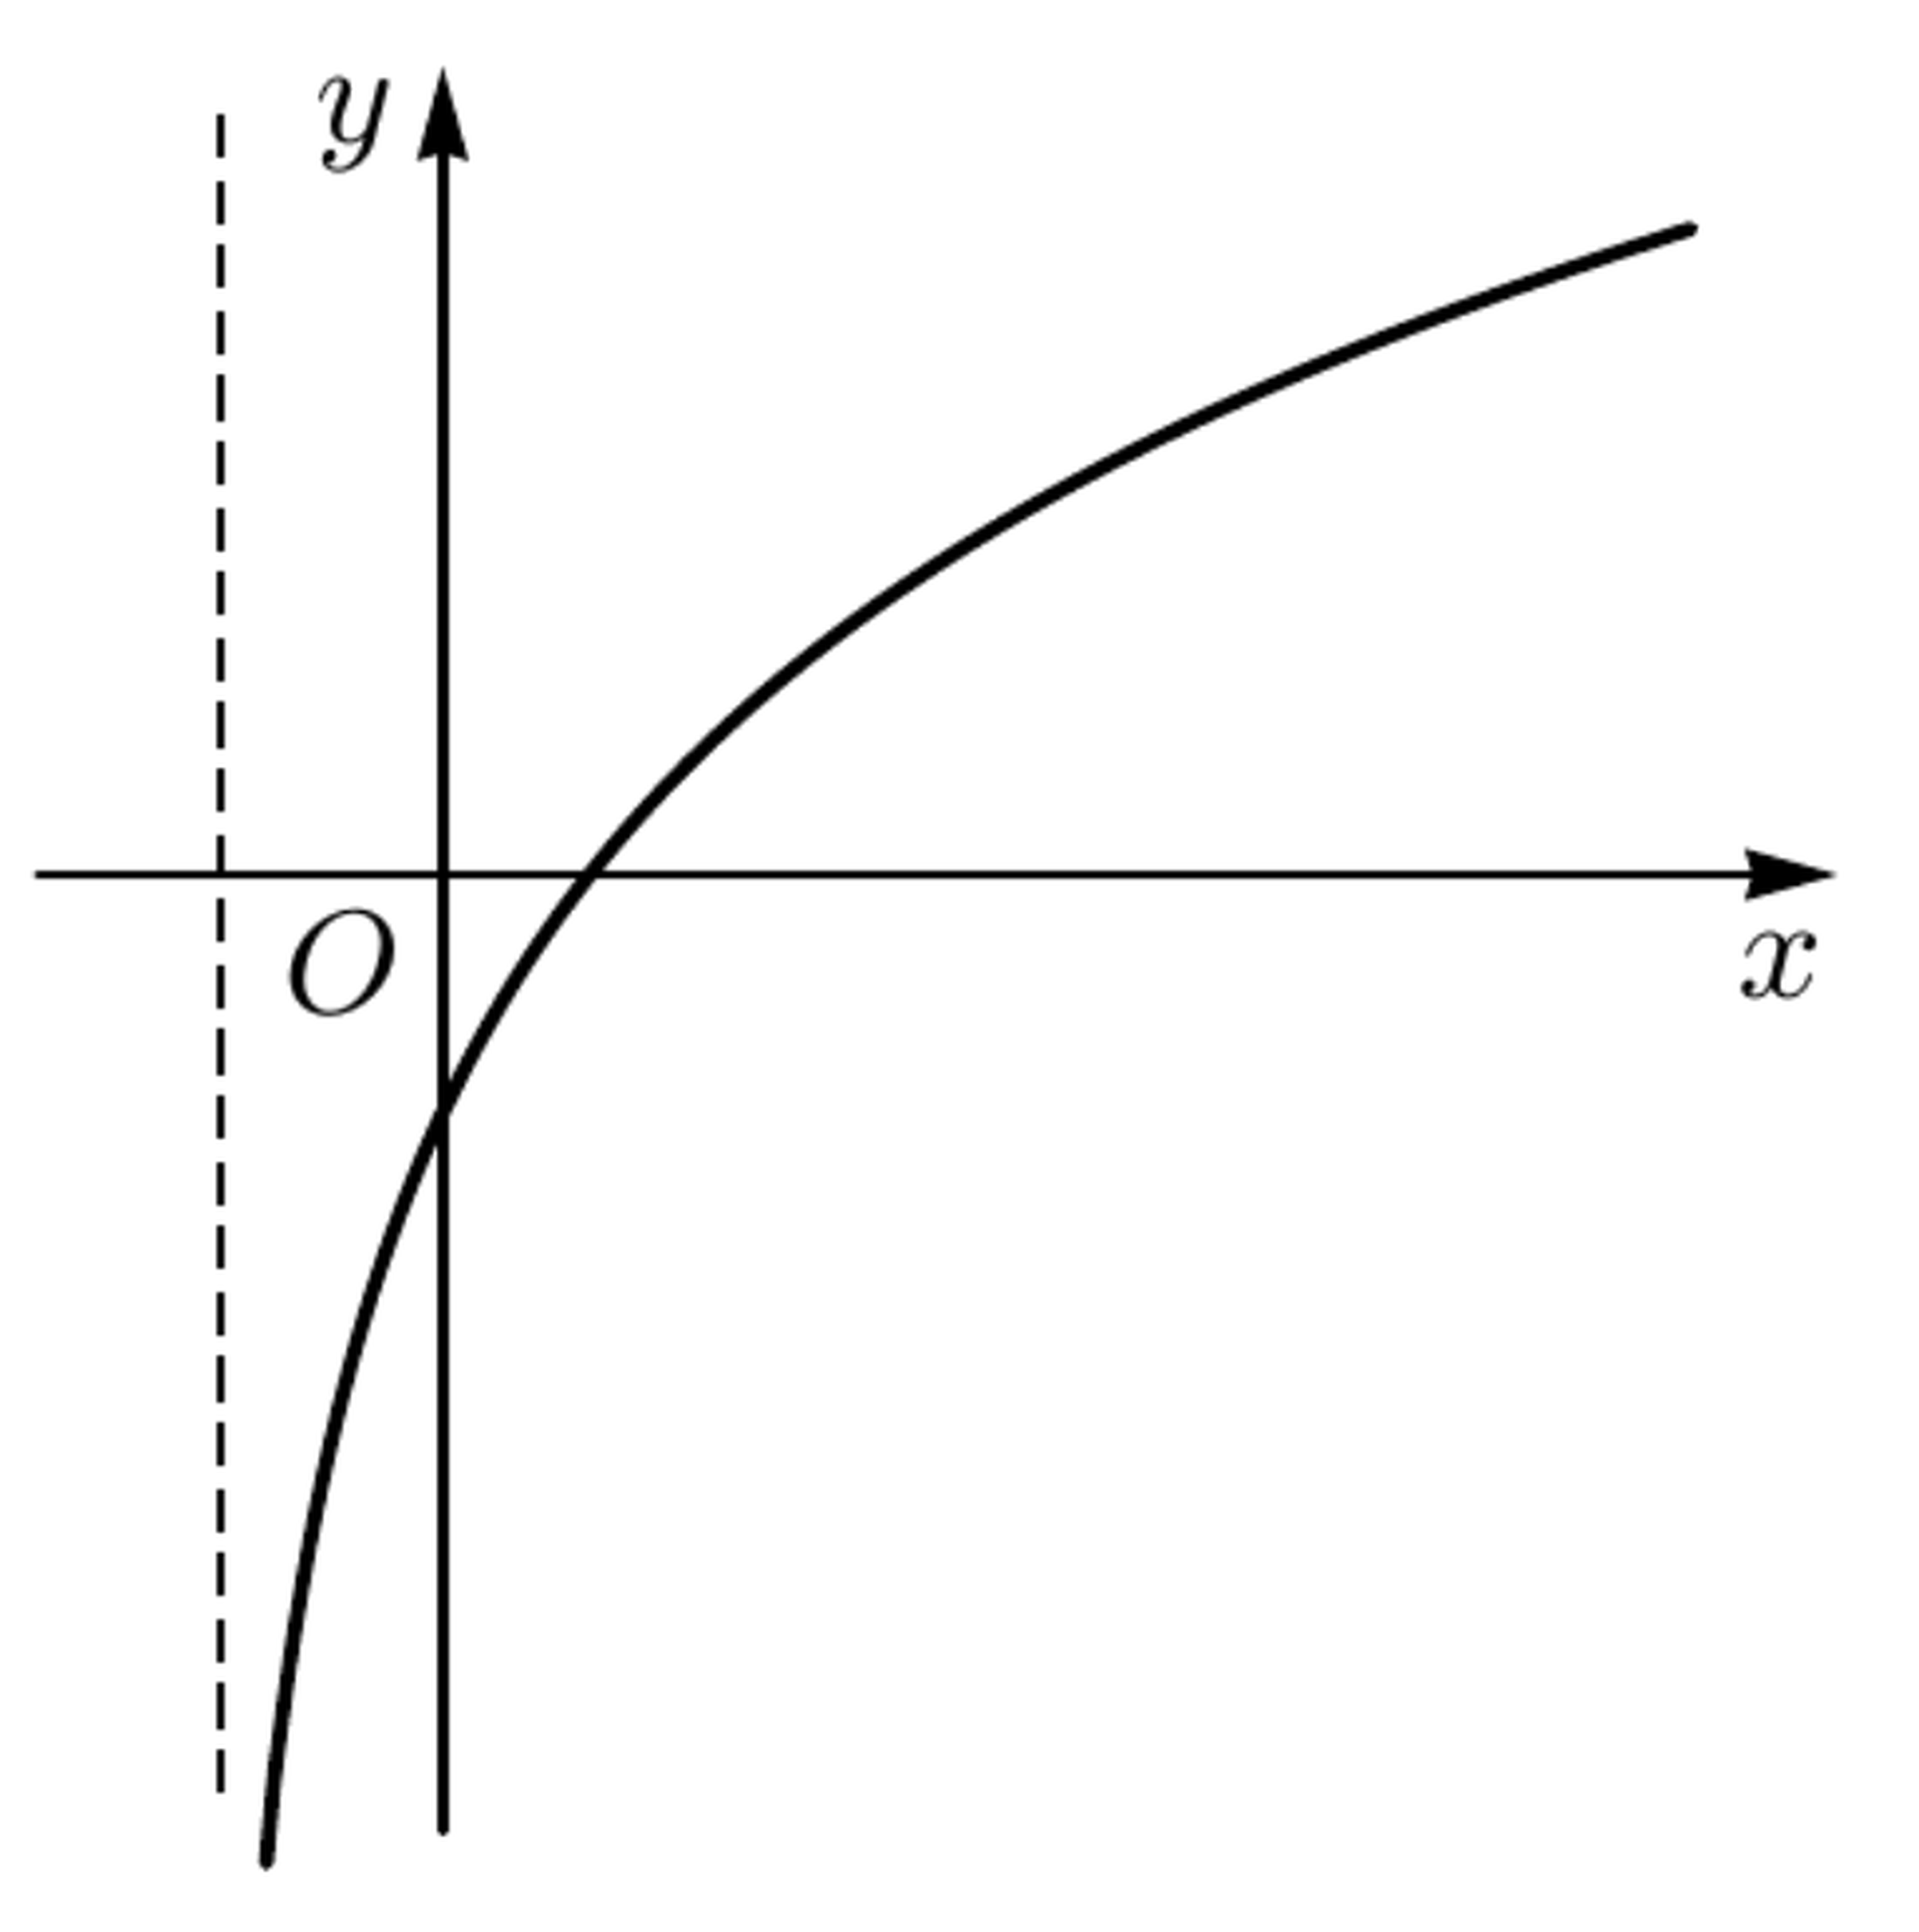
\includegraphics[width=0.42\textwidth]{figures/gao158_q15.png}
\end{center}

\keepwithprev
A. $a>1, b>1$\qquad\qquad B. $a>1, 0<b<1$

C. $0<a<1, b>1$\qquad\qquad D. $0<a<1, 0<b<1$

\ifanswer
\solbegin
\step{图像严格增，得 $a>1$.}
\step{图像与 $y$ 轴交于 $x$ 轴下方，得 $b>0$ 且 $\log_a b<0$，即 $0<b<1$，故选 $B$.}
\solend
\fi

% === Q16 === \lvert\log_2 x\rvert；解析 5 行，故选 C
\item 已知函数 $f(x)=\lvert\log_2 x\rvert$，若 $0<a<b$ 且 $f(a)=f(b)$，则 $a+2b$ 的取值范围是\mbox{（\quad）}

\keepwithprev
A. $(2\sqrt2,+\infty)$\qquad B. $[2\sqrt2,+\infty)$\qquad C. $(3,+\infty)$\qquad D. $[3,+\infty)$

\ifanswer
\solbegin
\step{由 $a<b$ 及 $\lvert\log_2 a\rvert=\lvert\log_2 b\rvert$，得 $\log_2 a=-\log_2 b$，即 $ab=1$，}
\step{且 $0<a<1<b$.}
\step{设 $t=a+2b=2b+\dfrac1b$，则 $t-3=\dfrac{(b-1)(2b-1)}{b}>0$.}
\step{反之，任取 $t>3$，令 $b=\dfrac{t+\sqrt{t^2-8}}{4}>1$、$a=\dfrac1b$，则满足题设且 $a+2b=t$.}
\step{因此取值范围为 $(3,+\infty)$，故选 $C$.}
\solend
\fi

\end{enumerate}

\bigsec{三、解答题}

\begin{enumerate}
\setcounter{enumi}{16}

% === Q17 === 集合、\overline{A}、\subseteq；解析 9 行
\item 已知全集 $U=\R$，集合 $A=\left\{x\mid\dfrac{x-3}{x+1}\leqslant0\right\}$，$B=\{x\mid x^2-2mx+m^2-9<0\}$（$m$ 为实数）.

(1) 当 $m=4$ 时，求 $A\cap B$ 和 $\overline{A}\cup B$；

(2) 若“$x\in A$”是“$x\in B$”的充分条件，求实数 $m$ 的取值范围.

\ifanswer
\solbegin
\step{(1) $\dfrac{x-3}{x+1}\leqslant0\Leftrightarrow-1<x\leqslant3$，所以 $A=(-1,3]$.}
\step{当 $m=4$ 时，$B=\{x\mid(x-4)^2<9\}=(1,7)$，}
\step{于是 $A\cap B=(1,3]$，$\overline{A}\cup B=(-\infty,-1]\cup(1,+\infty)$；}
\step{(2) $x^2-2mx+m^2-9<0\Leftrightarrow(x-m)^2<9$，所以 $B=(m-3,m+3)$.}
\step{题设充分条件等价于 $A\subseteq B$.}
\step{由于 $A=(-1,3]$，左端须满足 $m-3\leqslant-1$.}
\step{又 $3\in A$，须有 $3<m+3$.}
\step{这两个条件也保证 $(-1,3]\subseteq(m-3,m+3)$，}
\step{因此 $A\subseteq B\Leftrightarrow\begin{cases}m-3\leqslant-1\\m+3>3\end{cases}\Leftrightarrow0<m\leqslant2$.}
\solend
\fi

% === Q18 === 蓄水池造价（含 (3) 场地限制）；单位 \mathrm{m}；解析 13 行
\item 某工厂拟建一个容积为 $400\mathrm{m}^3$ 的无盖长方体蓄水池，池深 $4\mathrm{m}$，池底为矩形，其一边长
为 $x\mathrm{m}$. 池壁每平方米造价 100 元，池底每平方米造价 150 元. 设水池的总造价为 $C$
元.

(1) 把 $C$ 表示成 $x$ 的函数，并写出它的定义域；

(2) 当 $x$ 为何值时，总造价最低？最低造价是多少？

(3) 受场地限制，池底一边长 $x$ 不超过 $8\mathrm{m}$，此时总造价最低是多少？

\ifanswer
\solbegin
\step{(1) 设池底另一边长为 $y\mathrm{m}$，则 $4xy=400$，所以 $y=\dfrac{100}{x}$，$x>0$.}
\step{池底面积为 $100\mathrm{m}^2$，池壁总面积为 $8\left(x+\dfrac{100}{x}\right)\mathrm{m}^2$，}
\step{因此 $C(x)=100\times8\left(x+\dfrac{100}{x}\right)+150\times100=800x+\dfrac{80000}{x}+15000$，}
\step{定义域为 $(0,+\infty)$.}
\step{(2) 因为 $x>0$，所以 $C(x)=800\left(x+\dfrac{100}{x}\right)+15000$，}
\step{$\geqslant800\times2\sqrt{x\cdot\dfrac{100}{x}}+15000=31000$，}
\step{当且仅当 $x=\dfrac{100}{x}$，即 $x=10$ 时取等号.}
\step{答：当 $x=10$ 时，总造价最低，为 31000 元.}
\step{(3) 此时定义域为 $(0,8]$. 任取 $0<x_1<x_2\leqslant8$，}
\step{则 $C(x_2)-C(x_1)=800(x_2-x_1)\left(1-\dfrac{100}{x_1x_2}\right)<0$，}
\step{所以 $C(x)$ 在 $(0,8]$ 上严格递减，$x=8$ 时总造价最低，}
\step{且 $C(8)=800\times8+\dfrac{80000}{8}+15000=31400$.}
\step{答：受场地限制时，最低总造价为 31400 元.}
\solend
\fi

% === Q19 === 甲乙滤材 0.8^n／0.7^n；解析 17 行
\item 某环保公司研发了两种新型滤材甲和乙：污水每经过一层甲滤材，污染物含量减少
20\%；每经过一层乙滤材，污染物含量减少 30\%. 每层甲滤材成本 3 万元，每层乙滤材
成本 4 万元. 设原污水中污染物含量为 1，要求处理后污染物含量低于原来的 5\%.

(1) 若只使用一种滤材，污水经过 $n$ 层后污染物含量为 $y$，分别写出使用甲、乙两种滤材
时 $y$ 关于 $n$ 的函数关系式（$n$ 为正整数）；

(2) 若只使用一种滤材，分别求甲、乙至少各需要多少层，并比较哪种滤材的总成本更
低；

(3) 若两种滤材可以混合使用（先后顺序不影响效果），设使用甲滤材 $m$ 层、乙滤材 $n$
层（$m$、$n$ 为非负整数），求满足要求的最低总成本，并指出此时 $m$、$n$ 的值.

\ifanswer
\solbegin
\step{(1) 甲：$y=0.8^n$；乙：$y=0.7^n$，其中 $n$ 为正整数.}
\step{(2) 两种滤材均须满足 $y<0.05$，且污染物含量随层数增加而严格减少.}
\step{$0.8^{14}\approx0.04398<0.05<0.05498\approx0.8^{13}$，}
\step{$0.7^9=0.040353607<0.05<0.05764801=0.7^8$，}
\step{甲至少需要 14 层，成本为 $3\times14=42$ 万元；}
\step{乙至少需要 9 层，成本为 $4\times9=36$ 万元.}
\step{因此，只使用一种滤材时，使用乙滤材的总成本更低.}
\step{(3) 设总成本为 $C$ 万元，则 $C=3m+4n,0.8^m\cdot0.7^n<0.05,m,n\in\{0,1,2,\cdots\}$，}
\step{若 $m\geqslant3$，将其中 3 层甲替换为 2 层乙，}
\step{因为 $0.7^2=0.49<0.512=0.8^3,2\times4<3\times3$，}
\step{替换后污染物含量更低，成本减少 1 万元，因此最低成本方案必有 $m\leqslant2$.}
\step{当 $m=0$ 时，由第（2）小题得至少需要 9 层乙，最低成本为 36 万元.}
\step{当 $m=1$ 或 $m=2$ 时，$0.8\cdot0.7^7>0.8^2\cdot0.7^7=0.052706752>0.05$，}
\step{$0.8^2\cdot0.7^8<0.8\cdot0.7^8=0.046118408<0.05$，}
\step{因此两种情形均至少需要 8 层乙，}
\step{对应最低成本分别为 $3+4\times8=35$ 万元，$3\times2+4\times8=38$ 万元.}
\step{答：满足要求的最低总成本为 35 万元，此时使用甲滤材 1 层、乙滤材 8 层.}
\solend
\fi

% === Q20 === f(x)=\log_2(4^x+1)-x；\Delta；解析 17 行
\item 已知函数 $f(x)=\log_2(4^x+1)-x$.

(1) 证明 $f(x)=\log_2(2^x+2^{-x})$，并求 $f(x)$ 的最小值及取得最小值时 $x$ 的值；

(2) 解不等式 $f(x)>\log_2 5-1$；

(3) 证明：函数 $f(x)$ 在区间 $[0,+\infty)$ 上是严格增函数；并求使关于 $x$ 的方程 $f(x)=m$ 恰
有两个不同实数解的实数 $m$ 的取值范围.

\ifanswer
\solbegin
\step{(1) $f(x)=\log_2(4^x+1)-\log_2 2^x=\log_2\dfrac{4^x+1}{2^x}=\log_2(2^x+2^{-x})$，}
\step{因为 $2^x+2^{-x}\geqslant2\sqrt{2^x\cdot2^{-x}}=2$，所以 $f(x)\geqslant\log_2 2=1$，}
\step{等号当且仅当 $2^x=2^{-x}$，即 $x=0$ 时成立，故最小值为 1.}
\step{(2) 令 $t=2^x>0$，则 $f(x)>\log_2 5-1\Leftrightarrow t+\dfrac1t>\dfrac52\Leftrightarrow2t^2-5t+2>0$}
\step{$\Leftrightarrow(2t-1)(t-2)>0$，}
\step{结合 $t>0$，得 $0<t<\dfrac12$ 或 $t>2$，即 $x<-1$ 或 $x>1$，}
\step{解集为 $(-\infty,-1)\cup(1,+\infty)$.}
\step{(3) 任取 $0\leqslant x_1<x_2$，记 $a=2^{x_1}$，$b=2^{x_2}$，则 $1\leqslant a<b$，$ab>1$，}
\step{从而 $\left(b+\dfrac1b\right)-\left(a+\dfrac1a\right)=(b-a)\left(1-\dfrac{1}{ab}\right)>0$，}
\step{由对数函数的严格递增性，得 $f(x_1)<f(x_2)$，}
\step{所以 $f(x)$ 在 $[0,+\infty)$ 上是严格增函数.}
\step{当 $m<1$ 时，由（1）得方程无实数解；当 $m=1$ 时，只有实数解 $x=0$.}
\step{当 $m>1$ 时，令 $t=2^x>0$，则 $f(x)=m\Leftrightarrow t+\dfrac1t=2^m\Leftrightarrow t^2-2^m t+1=0$，}
\step{此时 $\Delta=2^{2m}-4>0$，两根之和为 $2^m>0$、之积为 $1>0$，}
\step{故有两个不同的正根.}
\step{每个正根 $t$ 唯一确定一个实数 $x=\log_2 t$，故原方程恰有两个不同实数解，}
\step{所求范围为 $m\in(1,+\infty)$.}
\solend
\fi

% === Q21 === f(x)=4^x-m\cdot2^{x+1}+3 值域与 h(m) 分段；解析 13 行
\item 已知函数 $f(x)=4^x-m\cdot2^{x+1}+3$（$m\in\R$），$x\in[0,2]$.

(1) 当 $m=1$ 时，求 $f(x)$ 的值域；

(2) 记 $f(x)$ 的最小值为 $h(m)$，求 $h(m)$ 的表达式；

(3) 若关于 $x$ 的方程 $f(x)=0$ 在区间 $[0,2]$ 上有解，求实数 $m$ 的取值范围.

\ifanswer
\solbegin
\step{令 $t=2^x$，则 $t\in[1,4]$，且 $f(x)=t^2-2mt+3=(t-m)^2+3-m^2$，}
\step{(1) 当 $m=1$ 时，$f(x)=(t-1)^2+2$.}
\step{由 $0\leqslant t-1\leqslant3$，得 $2\leqslant f(x)\leqslant11$，值域为 $[2,11]$.}
\step{(2) 二次函数 $y=(t-m)^2+3-m^2$ 的对称轴为直线 $t=m$.}
\step{当 $m\leqslant1$ 时，在 $t=1$ 处取最小值；}
\step{当 $1<m<4$ 时，在 $t=m$ 处取最小值；}
\step{当 $m\geqslant4$ 时，在 $t=4$ 处取最小值；}
\step{因此 $h(m)=\begin{cases}4-2m,&m\leqslant1\\3-m^2,&1<m<4\\19-8m,&m\geqslant4\end{cases}$；}
\step{(3) 方程 $f(x)=0$ 在 $[0,2]$ 上有解，}
\step{等价于存在 $t\in[1,4]$，使 $m=\dfrac{t^2+3}{2t}=\dfrac12\left(t+\dfrac3t\right)$，}
\step{由基本不等式，$m\geqslant\dfrac12\cdot2\sqrt{t\cdot\dfrac3t}=\sqrt3$，当且仅当 $t=\sqrt3$ 时取等号；}
\step{又 $\dfrac{19}{8}-m=\dfrac{(4-t)(4t-3)}{8t}\geqslant0$，当且仅当 $t=4$ 时取等号；}
\step{因此必有 $\sqrt3\leqslant m\leqslant\dfrac{19}{8}$.}
\solend
\fi

\end{enumerate}

\end{document}
"
%
% ① 原始材料：微信公众号"魔都数学加油站"文章，连载"27学年高一158"，原文标题
% "27学年高一158——2026-2027年上海市上实东滩高一上期中"（本卷本地编号 158 与
% 原卷连载号一致，无撞号）。
% 正文为 9 张 PNG 页（01/05/08/09 为 2560×3620，02/03/04/06/07 为 4762×6735，
% 同一篇各页分辨率混排，逐页按各自分辨率裁图核对）。
% 体例：讲评版——填空 3—12（10 题）、选择 13—16（4 题）、解答 17—21（5 题），
% 共 19 题，自第 3 题起编（1、2 未印在本篇）；Q5 只印【答案】、其余 18 题
% 逐题印【解析】（逐题核实，见 ②）。题目、答案、解析均据原图转录；卷面粉红色
% 水印"魔都数学加油站"及公众号页脚未录入。全卷末题为第 21 题，无附加题节。
% 全卷 2 组配图（逐页通读 9 页确认）——
%   · Q10 题干右侧"曼 → man"字形变换图（02 页），题目配图、三版都出，
%     裁 figures/gao158_q10.png；
%   · Q15 题干"如图所示"对数函数大致图像（03 页右下），题目配图、三版都出，
%     裁 figures/gao158_q15.png；
% 2 图均取自原卷截图，去粉色水印、转灰度、4× LANCZOS 放大；
% 其余各页逐页确认无其它题目配图、无解析内配图、无表格。
%
% 卷首标题：原卷印作"2026-2027 年上实东滩高一上期中"，年份区间按全稿惯例排 en dash；
% 原卷卷面未印副标题，本稿按同期中卷知识模块口径补出"集合与常用逻辑用语、不等式、函数"。
%
% ② 与原卷的排版差异／照录项清单：
%   ① 原文从第 3 题起，本稿保留原题号；共 19 题三节，解答题 5 题到 21；
%      三节各自一个 enumerate＋各自 \setcounter{enumi}{2}／{12}／{16}，
%      不贯穿（题目溯源.py 按 \bigsec 切节、每节独立计 depth，只收 depth==1 的 \item）；
%   ② 混合体例：Q5 只印【答案】、无【解析】，按 高一156 第 3 题成例另提
%      \ans{}、不补造解析；其余 18 题印【解析】、用 \solbegin…\solend；
%      四道选择题答案均在解析末句"故选 C／B／B／C"（逐个放大复核）、
%      题干括号 \mbox{（\quad）} 留空、不另提 \ans{}；答案版
%      【答案】/【解析】标记数 = 19 = 全卷题数（1 个 \ans ＋ 18 个 \solbegin）；
%   ③ 原卷卷面未印副标题，本稿按知识模块口径补出；
%   ④ 原卷填空横线按全稿惯例排 \blankline[4.4em]；选择题选项段前按惯例各加
%      \keepwithprev；解答题不留作答区、不加 \anspace（原卷为讲评版）；
%   ⑤ 数集：Q13"在 \R 上严格递增"、Q14"$x\in\R$"、Q17"$U=\R$"、
%      Q21"$m\in\R$" 原卷印正体粗体 R，按全稿惯例归一 \R；
%      绝对值排 \lvert…\rvert（Q12 $\lvert a\rvert$、Q14 $\lvert x-2\rvert$、
%      Q16 $\lvert\log_2 x\rvert$／$\lvert\log_2 a\rvert$／$\lvert\log_2 b\rvert$），
%      集合描述竖线排 \mid（Q17），不等号按全稿惯例排 \leqslant／\geqslant，
%      补集上划线 \overline{A}（Q17）；
%   ⑥ 子集／真子集符号逐处照录不统一：Q14 解析"$(2,3)\subsetneq(1,3)$"原卷印
%      带下划线且被斜杠划过的 ⊊（真子集，放大 03 页确认），照录 \subsetneq；
%      Q17 解析三处"$A\subseteq B$""$(-1,3]\subseteq(m-3,m+3)$"原卷印
%      带下划线 ⊆（放大 05 页确认），照录 \subseteq；本卷无单线 \subset 用例；
%   ⑦ 判别式：Q20 (3) 解析"$\Delta=2^{2m}-4>0$"原卷印高瘦等腰 \Delta
%      （像素实测高/宽 ≈ 1.13，扁三角 \triangle 为 0.93，放大 08 页确认），
%      照录 \Delta；本卷无扁三角 \triangle 用例；
%   ⑧ "图像"与"图象"：全卷统一用"图像"（Q6 题干、Q10 两处、Q11 解析、
%      Q15 题干与解析两处，逐处放大确认带单人旁），照录不改；
%   ⑨ 中文弯引号照录：Q5 命题"若实数…"、Q10"曼""man""新"、Q14 题干与
%      解析的两则不等式、Q17 (2)"$x\in A$""$x\in B$"；注释里一律 ASCII 引号；
%   ⑩ 半角逗号逐处照录：Q8"$2,3,4$""$-2,-1,0$"、Q10 点坐标 $(x,y)$／
%      $(t,2^t-1)$／$(1-2^t,t)$、Q15 四选项"$a>1, b>1$"等、
%      Q19 (3)"$C=3m+4n,0.8^m\cdot0.7^n<0.05,m,n\in\{0,1,2,\cdots\}$"
%      与"$0.7^2=0.49<0.512=0.8^3,2\times4<3\times3$"、
%      Q21 cases 内"$4-2m,$"等；其余行中逗号／顿号照录全角；
%      行末西文句点 ASCII `.`；
%   ⑪ 顿号照录：Q3"（用 $a$、$b$ 表示）"、Q5"$x$、$y$"、Q13"A、B"、
%      Q16 解析"$>1$、$a=\dfrac1b$"、Q19"甲、乙""$m$、$n$"、
%      Q20"$2^m>0$、之积为"、Q21"$m$、$n$"；顿号一律移到数学模式外，
%      数学模式内不出现中文标点；
%   ⑫ 角度与单位照录：Q10 三处"$90^{\circ}$"、Q18"$400\mathrm{m}^3$"
%      "$4\mathrm{m}$""$x\mathrm{m}$""$8\mathrm{m}$""$y\mathrm{m}$"
%      "$100\mathrm{m}^2$""$\left(x+\dfrac{100}{x}\right)\mathrm{m}^2$"；
%      Q19 百分号"20\%""30\%""5\%"按原卷排 \%；
%   ⑬ 文本模式全角括号照录：Q10"（提示：…）"、Q17"（$m$ 为实数）"、
%      Q19"（$n$ 为正整数）""（先后顺序不影响效果）""（$m$、$n$ 为非负整数）"、
%      Q20"由（1）得"、Q19"由第（2）小题"、Q21"（$m\in\R$）"；
%      子题行首标号按全稿惯例用半角 (1)(2)(3)；
%   ⑭ 复杂式照录别简化：Q3 $\dfrac{\log_3 2+\log_3 5}{\log_3 3+2\log_3 2}$、
%      Q8 $[-3,-2)\cup(4,5]$、Q9 $18ab=2^t\cdot3^t=6^t=a+b$、
%      Q12 $\dfrac{\sqrt6}{2}$、Q18 $C(8)=800\times8+\dfrac{80000}{8}+15000=31400$
%      （原卷即 C(8)，非 C(2)）、Q19 $0.8^{14}\approx0.04398$、
%      $0.7^9=0.040353607$、$0.052706752$、$0.046118408$、
%      Q20 $t^2-2^m t+1=0$、Q21 $h(m)$ 三段 cases 与 $\dfrac{(4-t)(4t-3)}{8t}$ 等；
%      \left…\right 不得拆到不同 $…$ 组；cases 块整体算一个印刷行；
%   ⑮ 一条 \step = 原卷解析的一个印刷行；别并折行、别拆行。跨页续印按题合并
%      （Q7 的 01—02 页、Q9/Q10/Q11 的 02—03 页、Q13/Q14 的 03 页上下、
%      Q15/Q16 的 04 页上下、Q17 的 04—05 页、Q18 的 05—06 页、
%      Q19 的 06—07 页、Q20 的 07—08 页、Q21 的 08—09 页）；
%      跨半页重叠行（Q5【答案】、Q9 设公共值行、Q10 题干、Q16 反之行、
%      Q18 (2) 题干、Q19 末两行、Q20 (3) 末行、Q21 cases 块）只算一个印刷行；
%   ⑯ 配图：2 组题目配图（见 ①），均三版都出，\needvspace 守卫放 \item 之前
%      把"题干＋图"整块推走，\includegraphics 放题干之后；本卷无解析内配图、
%      无红字加粗小标题（全卷逐页确认，故无 \stepm）。
%
% ③ 行数复核：一条 \step = 原卷解析的一个印刷行，cases 块作一个印刷行计。
%   逐题数（逐页核对）：Q3：1；Q4：2；Q5：0（只印【答案】、提 \ans{}，
%   不计入 \step 账）；Q6：1；Q7：4；Q8：5；Q9：2；Q10：2；Q11：3；
%   Q12：3；Q13：2；Q14：3；Q15：2；Q16：5；Q17：9；Q18：13；
%   Q19：17；Q20：17；Q21：13。
%   合计 104 行（104 条 \step ＋ 0 条 \stepm），与原卷逐题印刷行相等。
%   全卷 19 题：Q5 一处 \ans{} ＋ 其余 18 题设 \solbegin…\solend，
%   答案版【答案】/【解析】标记数 = 19 = 全卷题数。
%
% ④ 页码分布（供回原图复核）：
%   卷首标题＋"一、填空题"＋Q3 题干＋解析 1 行、Q4 题干＋解析 2 行、
%   Q5 题干＋【答案】在 01 页上半；Q5【答案】（重叠重印）＋Q6 题干＋解析 1 行、
%   Q7 题干＋解析前 3 行在 01 页下半；Q7 解析末行＋Q8 题干＋解析 5 行、
%   Q9 题干＋解析首行在 02 页上半；Q9 解析末行＋Q10 题干（含"曼→man"图）
%   ＋解析 2 行＋Q11 题干＋解析首行在 02 页下半；Q11 解析后 2 行＋Q12 题干
%   ＋解析 3 行＋"二、选择题"标题＋Q13 题干＋选项在 03 页上半；
%   Q13 选项（重叠重印）＋解析 2 行＋Q14 题干＋选项＋解析 3 行＋Q15 题干
%   ＋对数图像（右侧）在 03 页下半；Q15 选项＋解析 2 行＋Q16 题干＋选项
%   ＋解析前 4 行在 04 页上半；Q16 解析末行＋"三、解答题"标题＋Q17 题干
%   ＋两问＋解析 (1) 3 行在 04 页下半；Q17 解析 (2) 6 行＋Q18 题干＋三问
%   ＋解析 (1) 4 行＋(2) 首行在 05 页上下；Q18 解析 (2) 后 3 行＋(3) 5 行
%   ＋Q19 题干＋三问＋解析 (1) 1 行＋(2) 3 行在 06 页上下；Q19 解析 (2) 3 行
%   ＋(3) 12 行在 07 页上半；Q19 解析末 2 行（重叠）＋Q20 题干＋三问
%   ＋解析 (1) 3 行在 07 页下半；Q20 解析 (2) 4 行＋(3) 前 4 行在 08 页上半；
%   Q20 解析 (3) 后 6 行＋Q21 题干＋(1) 问在 08 页下半；Q21 (2)(3) 问＋
%   解析 (1) 3 行＋(2) 5 行＋cases 块在 09 页上半；Q21 cases 块（重叠）
%   ＋(3) 解析 5 行在 09 页下半。本稿按题连排，不丢行、不并折行；
%   全卷末题为第 21 题，无附加题节。
%
% ⑤ 存疑／需主会话回原图复核：
%   1. Q14 解析"$(2,3)\subsetneq(1,3)$"的 ⊊（真子集带斜杠）与 Q17 的 ⊆
%      是两种不同记号，本稿分别照录 \subsetneq／\subseteq，请复核；
%   2. Q20 (3)"$\Delta=2^{2m}-4>0$"判为高瘦 \Delta，请复核是否 \triangle；
%   3. 任务书提示"Q18 解析里印 C(2)=…"，但 06 页原图逐处读作
%      $C(8)=800\times8+\dfrac{80000}{8}+15000=31400$，未找到 C(2)，
%      本稿照原卷排 C(8)，请复核；
%   4. Q19 解析末句"最低总成本为 35 万元"（07 页上下两处印同），
%      OCR 曾误读为 34，本稿按 35 照录，请复核；
%   5. Q10 提示末尾"坐标为 $(-y,x)$）."为半角 $)$＋全角 $）$ 两枚括号，
%      本稿照录，请复核；
%   6. Q21 cases 块后"；"落在分式中行右侧（排版居中基线所致），
%      本稿排作 $…\end{cases}$；，请复核。
%   全卷除此 6 类外未发现其它笔误／自相矛盾处；19 题中 18 题印【解析】。
%
\documentclass[a4paper,11pt]{article}
\usepackage{common}

\begin{document}

\examtitlest[3]{2026--2027 年上实东滩高一上期中}{集合与常用逻辑用语、不等式、函数}

\bigsec{一、填空题}

\begin{enumerate}
\setcounter{enumi}{2}

% === Q3 === 换底公式；解析 1 行
\item 已知 $3^a=5$，$\log_3 2=b$，则 $\log_{12} 10=$\blankline[4.4em]（用 $a$、$b$ 表示）.

\ifanswer
\solbegin
\step{$\log_{12} 10=\dfrac{\log_3 2+\log_3 5}{\log_3 3+2\log_3 2}=\dfrac{a+b}{1+2b}$.}
\solend
\fi

% === Q4 === 定义域；解析 2 行；半角括号 ( ) 与全角逗号照录
\item 函数 $y=\sqrt{2-x}+\lg(x^2-1)$ 的定义域为\blankline[4.4em].

\ifanswer
\solbegin
\step{由 $2-x\geqslant0$ 且 $x^2-1>0$，得 $x\leqslant2$ 且 ($x<-1$或$x>1$)，}
\step{定义域为 $(-\infty,-1)\cup(1,2]$.}
\solend
\fi

% === Q5 === 只印【答案】、无【解析】；反证法，中文弯引号
\item 用反证法证明命题“若实数 $x$、$y$ 满足 $x+y>2$，则 $x$、$y$ 中至少有一个大于 1”时，
应假设\blankline[4.4em].

\ifanswer
\ans{$x\leqslant1$ 且 $y\leqslant1$}
\fi

% === Q6 === 图像平移；解析 1 行
\item 函数 $y=\dfrac{2x+1}{x-1}$ 的图像可由函数 $y=\dfrac{3}{x}$ 的图像先向右平移 $a$ 个单位，再向上平移 $b$ 个单位
得到，则 $a+b=$\blankline[4.4em].

\ifanswer
\solbegin
\step{$y=\dfrac{2x+1}{x-1}=\dfrac{3}{x-1}+2$，所以 $a=1$，$b=2$，$a+b=3$.}
\solend
\fi

% === Q7 === 集合三元子集；解析 4 行，跨 01—02 页
\item 设 $A=\{a_1,a_2,a_3,a_4\}$ 是由四个实数组成的集合，若 $A$ 的所有三元子集中，三个元素之和
组成的集合为 $B=\{1,4,7,12\}$，则集合 $A=$\blankline[4.4em].

\ifanswer
\solbegin
\step{设 $S=a_1+a_2+a_3+a_4$，}
\step{每个元素在四个三元子集中恰出现三次，则 $3S=1+4+7+12=24$，得 $S=8$.}
\step{四个三元子集的元素和分别为 $S-a_i$，}
\step{所以 $A=\{8-1,8-4,8-7,8-12\}=\{-4,1,4,7\}$.}
\solend
\fi

% === Q8 === 不等式整数解；解析 5 行；半角逗号照录
\item 不等式 $x^2-(a+1)x+a<0$ 的解集中恰有 3 个整数，则 $a$ 的取值范围是\blankline[4.4em].

\ifanswer
\solbegin
\step{原不等式为 $(x-1)(x-a)<0$；}
\step{$a=1$ 时解集为空集，不符合题意.}
\step{若 $a>1$，解集为 $(1,a)$，恰含整数 $2,3,4$，则 $4<a\leqslant5$.}
\step{若 $a<1$，解集为 $(a,1)$，恰含整数 $-2,-1,0$，则 $-3\leqslant a<-2$.}
\step{故 $a$ 的取值范围是 $[-3,-2)\cup(4,5]$.}
\solend
\fi

% === Q9 === 对数换底＋指数；解析 2 行
\item 已知正数 $a$、$b$ 满足 $1+\log_2 a=2+\log_3 b=\log_6(a+b)$，则 $\dfrac1a+\dfrac1b=$\blankline[4.4em].

\ifanswer
\solbegin
\step{设公共值为 $t$，则 $2a=2^t$，$9b=3^t$，$a+b=6^t$，}
\step{于是 $18ab=2^t\cdot3^t=6^t=a+b$，即 $\dfrac1a+\dfrac1b=\dfrac{a+b}{ab}=18$.}
\solend
\fi

% === Q10 === "曼"字旋转 90°；题目配图（三版都出）；解析 2 行
\needvspace{6cm}
\item 网上流传一个有趣的字形变换：把汉字“曼”的右半部分旋转 $90^{\circ}$，就得到英文单词
“man”的艺术字. 数学中，把曲线绕原点旋转也会得到“新”的曲线：将函数
$y=2^x-1$ 的图像绕坐标原点 $O$ 逆时针旋转 $90^{\circ}$，得到的曲线恰是某个函数的
图像，则这个函数的解析式为\blankline[4.4em]（提示：点 $(x,y)$ 绕 $O$ 逆时针旋转 $90^{\circ}$ 后的
坐标为 $(-y,x)$）.

\begin{center}

\includegraphics[width=0.42\textwidth]{figures/gao158_q10.png}
\end{center}

\ifanswer
\solbegin
\step{原图像上的点 $(t,2^t-1)$ 旋转后为 $(1-2^t,t)$.}
\step{记其为 $(x,y)$，则 $x=1-2^y$，即 $y=\log_2(1-x)$，定义域为 $(-\infty,1)$.}
\solend
\fi

% === Q11 === 值域；解析 3 行，跨 02—03 页
\item 函数 $f(x)=\sqrt{x-2}-\sqrt{15-3x}$ 的值域为\blankline[4.4em].

\ifanswer
\solbegin
\step{由 $x-2\geqslant0$ 且 $15-3x\geqslant0$，得定义域为 $[2,5]$.}
\step{在 $[2,5]$ 上，$\sqrt{x-2}$ 与 $-\sqrt{15-3x}$ 均严格递增，因此 $f(x)$ 严格递增.}
\step{$f(2)=-3$，$f(5)=\sqrt3$，结合函数的图像，值域为 $[-3,\sqrt3]$.}
\solend
\fi

% === Q12 === 绝对值 \lvert…\rvert；解析 3 行
\item 设实数 $a$ 满足 $a<4a^3-5a<\lvert a\rvert$，则 $a$ 的取值范围是\blankline[4.4em].

\ifanswer
\solbegin
\step{由 $a<\lvert a\rvert$ 得 $a<0$，原不等式为 $a<4a^3-5a<-a$.}
\step{同除以 $a<0$，得 $1>4a^2-5>-1\Leftrightarrow1<a^2<\dfrac32$，结合 $a<0$，}
\step{得 $-\dfrac{\sqrt6}{2}<a<-1$，故解集为 $\left(-\dfrac{\sqrt6}{2},-1\right)$.}
\solend
\fi

\end{enumerate}

\bigsec{二、选择题}

\begin{enumerate}
\setcounter{enumi}{12}

% === Q13 === \R 归一；解析 2 行，故选 C
\item 已知 $a>b$，则下列不等式一定成立的是\mbox{（\quad）}

\keepwithprev
A. $\dfrac1a<\dfrac1b$\qquad B. $a^2>b^2$\qquad C. $a^3>b^3$\qquad D. $ac^2>bc^2$

\ifanswer
\solbegin
\step{幂函数 $y=x^3$ 在 $\R$ 上严格递增，$a>b\Rightarrow a^3>b^3$，C 正确.}
\step{取 $a=1$，$b=-1$ 得 A、B 不成立；取 $c=0$ 得 D 不成立；故选 $C$.}
\solend
\fi

% === Q14 === \subsetneq 真子集；解析 3 行，故选 B
\item 设 $x\in\R$，则“$\lvert x-2\rvert<1$”是“$x^2-5x+6<0$”的\mbox{（\quad）}

\keepwithprev
A. 充分非必要条件\qquad\qquad B. 必要非充分条件

C. 充要条件\qquad\qquad D. 既非充分又非必要条件

\ifanswer
\solbegin
\step{$\lvert x-2\rvert<1\Leftrightarrow1<x<3$，$x^2-5x+6<0\Leftrightarrow(x-2)(x-3)<0\Leftrightarrow2<x<3$.}
\step{由 $(2,3)\subsetneq(1,3)$，得“$\lvert x-2\rvert<1$”是“$x^2-5x+6<0$”的必要非充分条件，}
\step{故选 $B$.}
\solend
\fi

% === Q15 === 对数函数大致图像（题目配图，三版都出）；解析 2 行，故选 B
\needvspace{9cm}
\item 已知函数 $f(x)=\log_a(x+b)$（$a>0$ 且 $a\ne1$）的大致图像如图所示，则 $a$、$b$ 满足
的关系是\mbox{（\quad）}

\begin{center}
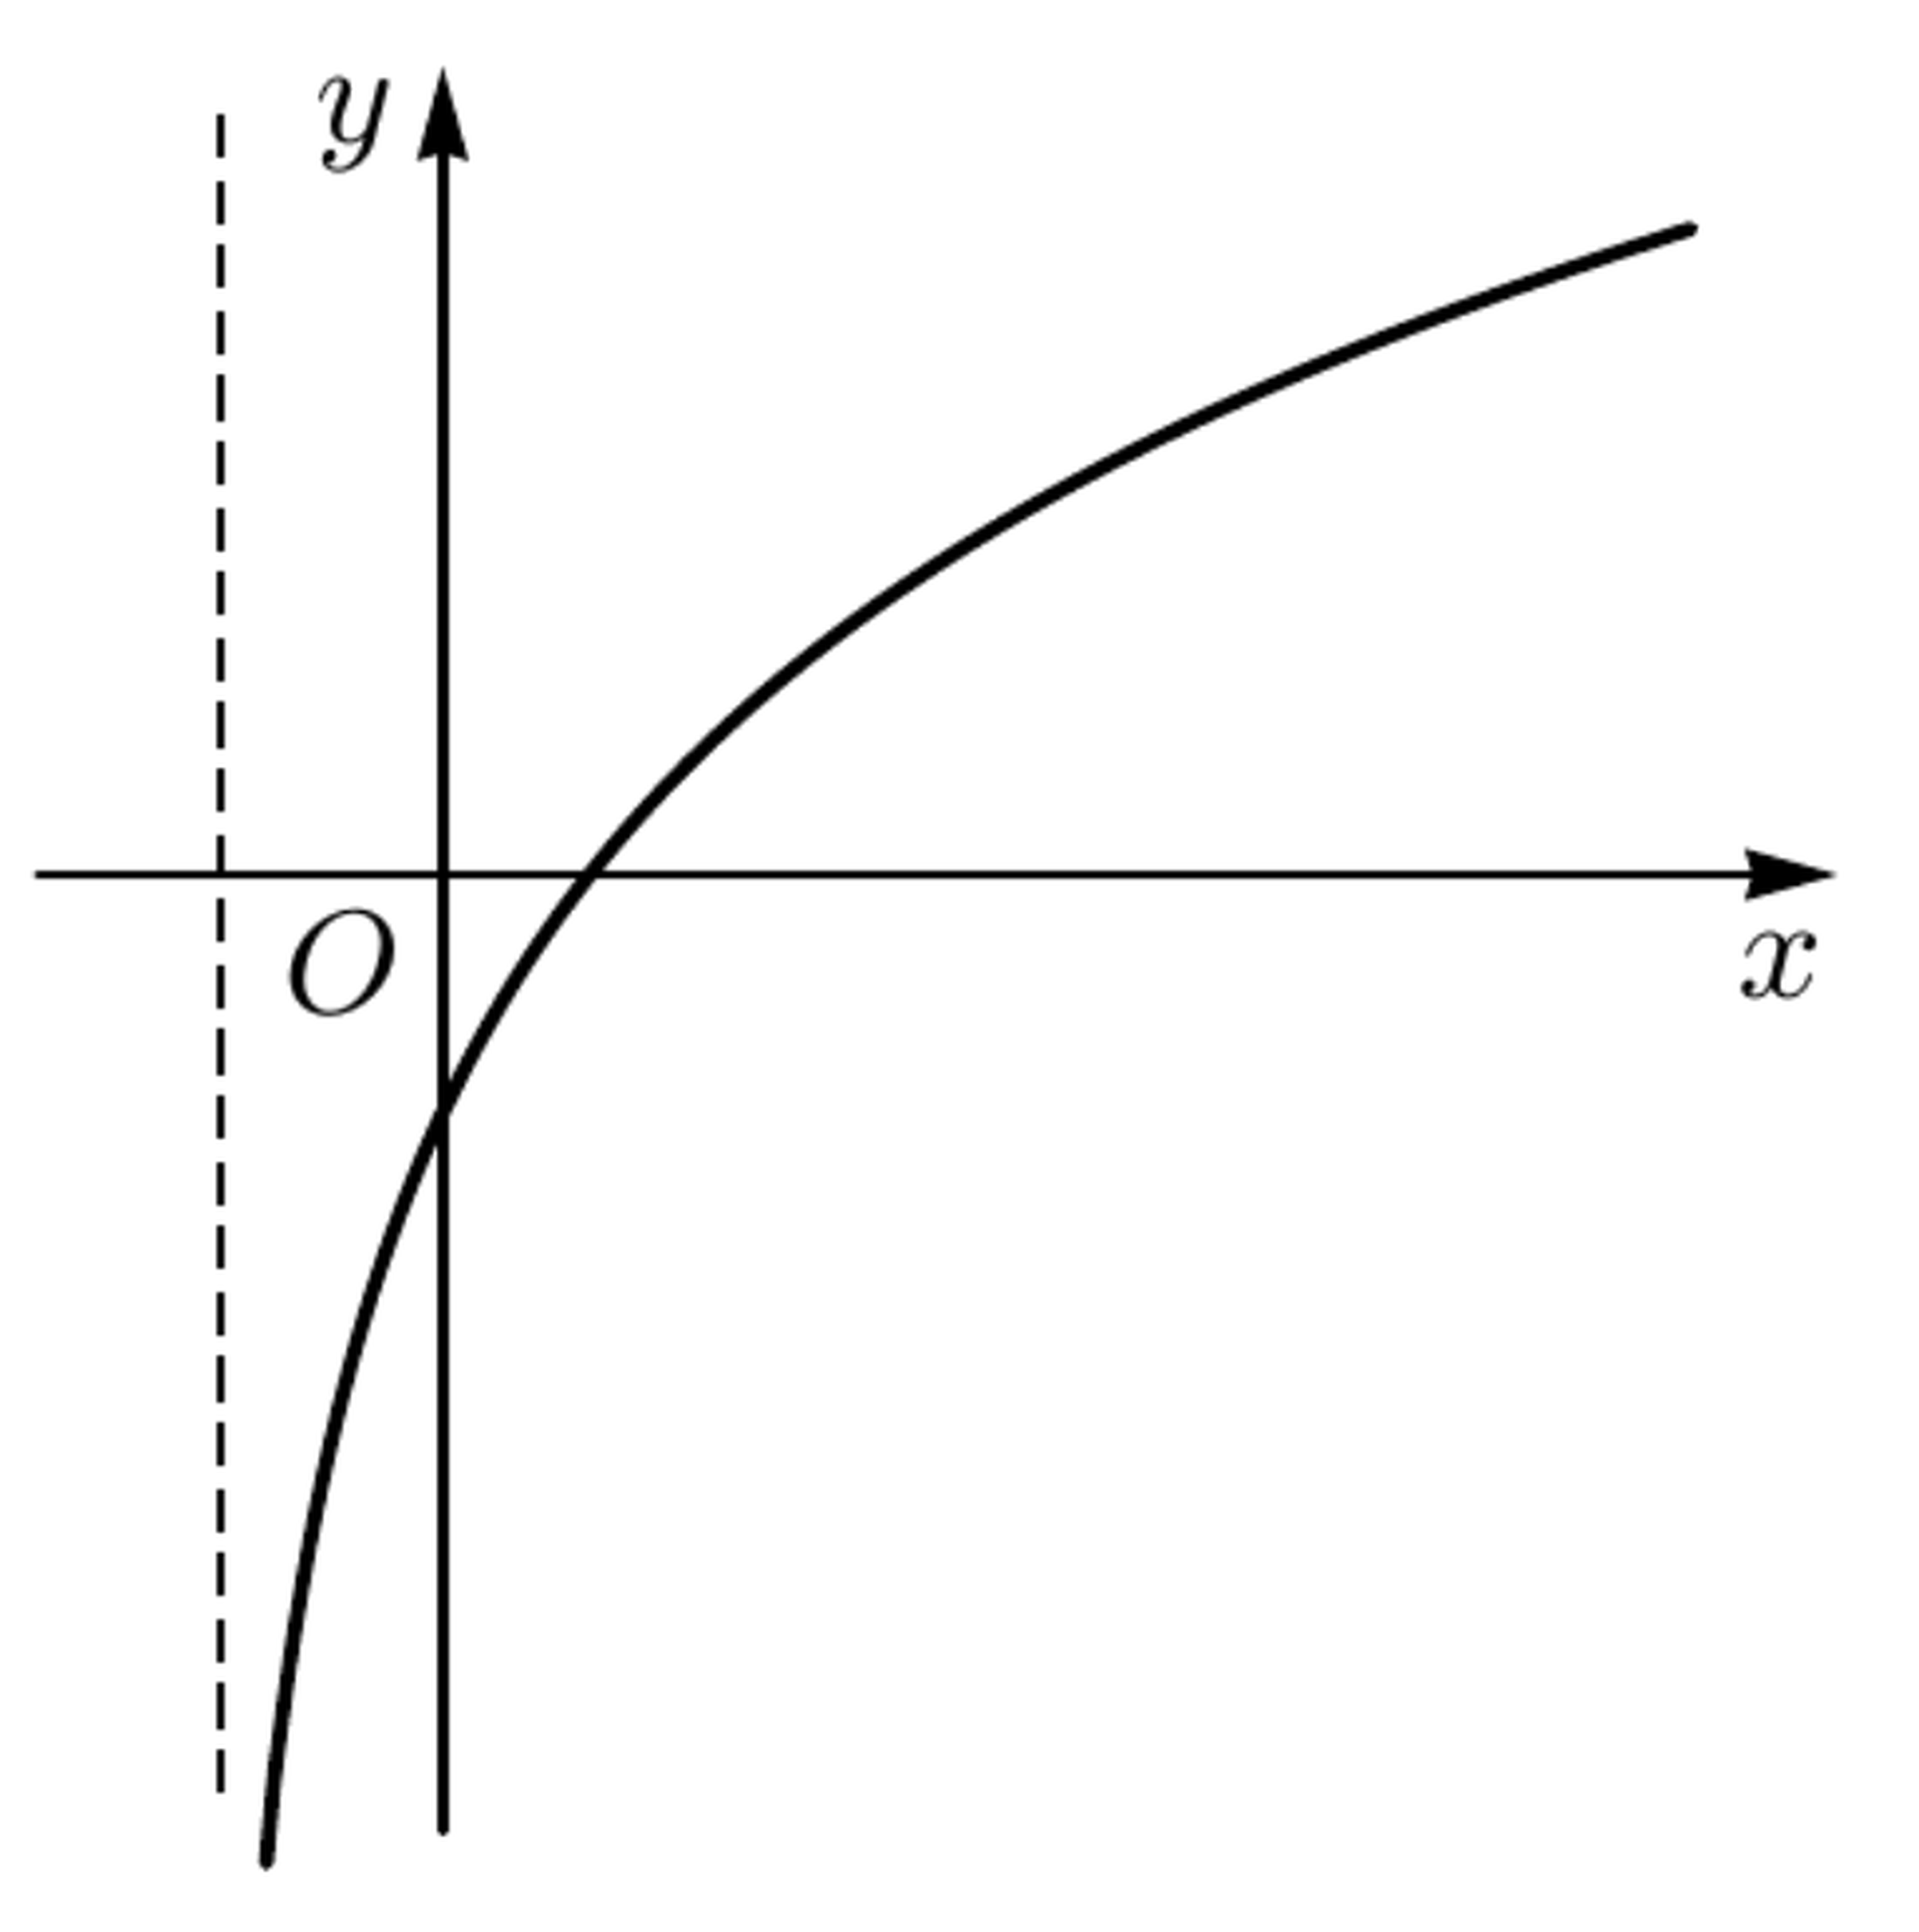
\includegraphics[width=0.42\textwidth]{figures/gao158_q15.png}
\end{center}

\keepwithprev
A. $a>1, b>1$\qquad\qquad B. $a>1, 0<b<1$

C. $0<a<1, b>1$\qquad\qquad D. $0<a<1, 0<b<1$

\ifanswer
\solbegin
\step{图像严格增，得 $a>1$.}
\step{图像与 $y$ 轴交于 $x$ 轴下方，得 $b>0$ 且 $\log_a b<0$，即 $0<b<1$，故选 $B$.}
\solend
\fi

% === Q16 === \lvert\log_2 x\rvert；解析 5 行，故选 C
\item 已知函数 $f(x)=\lvert\log_2 x\rvert$，若 $0<a<b$ 且 $f(a)=f(b)$，则 $a+2b$ 的取值范围是\mbox{（\quad）}

\keepwithprev
A. $(2\sqrt2,+\infty)$\qquad B. $[2\sqrt2,+\infty)$\qquad C. $(3,+\infty)$\qquad D. $[3,+\infty)$

\ifanswer
\solbegin
\step{由 $a<b$ 及 $\lvert\log_2 a\rvert=\lvert\log_2 b\rvert$，得 $\log_2 a=-\log_2 b$，即 $ab=1$，}
\step{且 $0<a<1<b$.}
\step{设 $t=a+2b=2b+\dfrac1b$，则 $t-3=\dfrac{(b-1)(2b-1)}{b}>0$.}
\step{反之，任取 $t>3$，令 $b=\dfrac{t+\sqrt{t^2-8}}{4}>1$、$a=\dfrac1b$，则满足题设且 $a+2b=t$.}
\step{因此取值范围为 $(3,+\infty)$，故选 $C$.}
\solend
\fi

\end{enumerate}

\bigsec{三、解答题}

\begin{enumerate}
\setcounter{enumi}{16}

% === Q17 === 集合、\overline{A}、\subseteq；解析 9 行
\item 已知全集 $U=\R$，集合 $A=\left\{x\mid\dfrac{x-3}{x+1}\leqslant0\right\}$，$B=\{x\mid x^2-2mx+m^2-9<0\}$（$m$ 为实数）.

(1) 当 $m=4$ 时，求 $A\cap B$ 和 $\overline{A}\cup B$；

(2) 若“$x\in A$”是“$x\in B$”的充分条件，求实数 $m$ 的取值范围.

\ifanswer
\solbegin
\step{(1) $\dfrac{x-3}{x+1}\leqslant0\Leftrightarrow-1<x\leqslant3$，所以 $A=(-1,3]$.}
\step{当 $m=4$ 时，$B=\{x\mid(x-4)^2<9\}=(1,7)$，}
\step{于是 $A\cap B=(1,3]$，$\overline{A}\cup B=(-\infty,-1]\cup(1,+\infty)$；}
\step{(2) $x^2-2mx+m^2-9<0\Leftrightarrow(x-m)^2<9$，所以 $B=(m-3,m+3)$.}
\step{题设充分条件等价于 $A\subseteq B$.}
\step{由于 $A=(-1,3]$，左端须满足 $m-3\leqslant-1$.}
\step{又 $3\in A$，须有 $3<m+3$.}
\step{这两个条件也保证 $(-1,3]\subseteq(m-3,m+3)$，}
\step{因此 $A\subseteq B\Leftrightarrow\begin{cases}m-3\leqslant-1\\m+3>3\end{cases}\Leftrightarrow0<m\leqslant2$.}
\solend
\fi

% === Q18 === 蓄水池造价（含 (3) 场地限制）；单位 \mathrm{m}；解析 13 行
\item 某工厂拟建一个容积为 $400\mathrm{m}^3$ 的无盖长方体蓄水池，池深 $4\mathrm{m}$，池底为矩形，其一边长
为 $x\mathrm{m}$. 池壁每平方米造价 100 元，池底每平方米造价 150 元. 设水池的总造价为 $C$
元.

(1) 把 $C$ 表示成 $x$ 的函数，并写出它的定义域；

(2) 当 $x$ 为何值时，总造价最低？最低造价是多少？

(3) 受场地限制，池底一边长 $x$ 不超过 $8\mathrm{m}$，此时总造价最低是多少？

\ifanswer
\solbegin
\step{(1) 设池底另一边长为 $y\mathrm{m}$，则 $4xy=400$，所以 $y=\dfrac{100}{x}$，$x>0$.}
\step{池底面积为 $100\mathrm{m}^2$，池壁总面积为 $8\left(x+\dfrac{100}{x}\right)\mathrm{m}^2$，}
\step{因此 $C(x)=100\times8\left(x+\dfrac{100}{x}\right)+150\times100=800x+\dfrac{80000}{x}+15000$，}
\step{定义域为 $(0,+\infty)$.}
\step{(2) 因为 $x>0$，所以 $C(x)=800\left(x+\dfrac{100}{x}\right)+15000$，}
\step{$\geqslant800\times2\sqrt{x\cdot\dfrac{100}{x}}+15000=31000$，}
\step{当且仅当 $x=\dfrac{100}{x}$，即 $x=10$ 时取等号.}
\step{答：当 $x=10$ 时，总造价最低，为 31000 元.}
\step{(3) 此时定义域为 $(0,8]$. 任取 $0<x_1<x_2\leqslant8$，}
\step{则 $C(x_2)-C(x_1)=800(x_2-x_1)\left(1-\dfrac{100}{x_1x_2}\right)<0$，}
\step{所以 $C(x)$ 在 $(0,8]$ 上严格递减，$x=8$ 时总造价最低，}
\step{且 $C(8)=800\times8+\dfrac{80000}{8}+15000=31400$.}
\step{答：受场地限制时，最低总造价为 31400 元.}
\solend
\fi

% === Q19 === 甲乙滤材 0.8^n／0.7^n；解析 17 行
\item 某环保公司研发了两种新型滤材甲和乙：污水每经过一层甲滤材，污染物含量减少
20\%；每经过一层乙滤材，污染物含量减少 30\%. 每层甲滤材成本 3 万元，每层乙滤材
成本 4 万元. 设原污水中污染物含量为 1，要求处理后污染物含量低于原来的 5\%.

(1) 若只使用一种滤材，污水经过 $n$ 层后污染物含量为 $y$，分别写出使用甲、乙两种滤材
时 $y$ 关于 $n$ 的函数关系式（$n$ 为正整数）；

(2) 若只使用一种滤材，分别求甲、乙至少各需要多少层，并比较哪种滤材的总成本更
低；

(3) 若两种滤材可以混合使用（先后顺序不影响效果），设使用甲滤材 $m$ 层、乙滤材 $n$
层（$m$、$n$ 为非负整数），求满足要求的最低总成本，并指出此时 $m$、$n$ 的值.

\ifanswer
\solbegin
\step{(1) 甲：$y=0.8^n$；乙：$y=0.7^n$，其中 $n$ 为正整数.}
\step{(2) 两种滤材均须满足 $y<0.05$，且污染物含量随层数增加而严格减少.}
\step{$0.8^{14}\approx0.04398<0.05<0.05498\approx0.8^{13}$，}
\step{$0.7^9=0.040353607<0.05<0.05764801=0.7^8$，}
\step{甲至少需要 14 层，成本为 $3\times14=42$ 万元；}
\step{乙至少需要 9 层，成本为 $4\times9=36$ 万元.}
\step{因此，只使用一种滤材时，使用乙滤材的总成本更低.}
\step{(3) 设总成本为 $C$ 万元，则 $C=3m+4n,0.8^m\cdot0.7^n<0.05,m,n\in\{0,1,2,\cdots\}$，}
\step{若 $m\geqslant3$，将其中 3 层甲替换为 2 层乙，}
\step{因为 $0.7^2=0.49<0.512=0.8^3,2\times4<3\times3$，}
\step{替换后污染物含量更低，成本减少 1 万元，因此最低成本方案必有 $m\leqslant2$.}
\step{当 $m=0$ 时，由第（2）小题得至少需要 9 层乙，最低成本为 36 万元.}
\step{当 $m=1$ 或 $m=2$ 时，$0.8\cdot0.7^7>0.8^2\cdot0.7^7=0.052706752>0.05$，}
\step{$0.8^2\cdot0.7^8<0.8\cdot0.7^8=0.046118408<0.05$，}
\step{因此两种情形均至少需要 8 层乙，}
\step{对应最低成本分别为 $3+4\times8=35$ 万元，$3\times2+4\times8=38$ 万元.}
\step{答：满足要求的最低总成本为 35 万元，此时使用甲滤材 1 层、乙滤材 8 层.}
\solend
\fi

% === Q20 === f(x)=\log_2(4^x+1)-x；\Delta；解析 17 行
\item 已知函数 $f(x)=\log_2(4^x+1)-x$.

(1) 证明 $f(x)=\log_2(2^x+2^{-x})$，并求 $f(x)$ 的最小值及取得最小值时 $x$ 的值；

(2) 解不等式 $f(x)>\log_2 5-1$；

(3) 证明：函数 $f(x)$ 在区间 $[0,+\infty)$ 上是严格增函数；并求使关于 $x$ 的方程 $f(x)=m$ 恰
有两个不同实数解的实数 $m$ 的取值范围.

\ifanswer
\solbegin
\step{(1) $f(x)=\log_2(4^x+1)-\log_2 2^x=\log_2\dfrac{4^x+1}{2^x}=\log_2(2^x+2^{-x})$，}
\step{因为 $2^x+2^{-x}\geqslant2\sqrt{2^x\cdot2^{-x}}=2$，所以 $f(x)\geqslant\log_2 2=1$，}
\step{等号当且仅当 $2^x=2^{-x}$，即 $x=0$ 时成立，故最小值为 1.}
\step{(2) 令 $t=2^x>0$，则 $f(x)>\log_2 5-1\Leftrightarrow t+\dfrac1t>\dfrac52\Leftrightarrow2t^2-5t+2>0$}
\step{$\Leftrightarrow(2t-1)(t-2)>0$，}
\step{结合 $t>0$，得 $0<t<\dfrac12$ 或 $t>2$，即 $x<-1$ 或 $x>1$，}
\step{解集为 $(-\infty,-1)\cup(1,+\infty)$.}
\step{(3) 任取 $0\leqslant x_1<x_2$，记 $a=2^{x_1}$，$b=2^{x_2}$，则 $1\leqslant a<b$，$ab>1$，}
\step{从而 $\left(b+\dfrac1b\right)-\left(a+\dfrac1a\right)=(b-a)\left(1-\dfrac{1}{ab}\right)>0$，}
\step{由对数函数的严格递增性，得 $f(x_1)<f(x_2)$，}
\step{所以 $f(x)$ 在 $[0,+\infty)$ 上是严格增函数.}
\step{当 $m<1$ 时，由（1）得方程无实数解；当 $m=1$ 时，只有实数解 $x=0$.}
\step{当 $m>1$ 时，令 $t=2^x>0$，则 $f(x)=m\Leftrightarrow t+\dfrac1t=2^m\Leftrightarrow t^2-2^m t+1=0$，}
\step{此时 $\Delta=2^{2m}-4>0$，两根之和为 $2^m>0$、之积为 $1>0$，}
\step{故有两个不同的正根.}
\step{每个正根 $t$ 唯一确定一个实数 $x=\log_2 t$，故原方程恰有两个不同实数解，}
\step{所求范围为 $m\in(1,+\infty)$.}
\solend
\fi

% === Q21 === f(x)=4^x-m\cdot2^{x+1}+3 值域与 h(m) 分段；解析 13 行
\item 已知函数 $f(x)=4^x-m\cdot2^{x+1}+3$（$m\in\R$），$x\in[0,2]$.

(1) 当 $m=1$ 时，求 $f(x)$ 的值域；

(2) 记 $f(x)$ 的最小值为 $h(m)$，求 $h(m)$ 的表达式；

(3) 若关于 $x$ 的方程 $f(x)=0$ 在区间 $[0,2]$ 上有解，求实数 $m$ 的取值范围.

\ifanswer
\solbegin
\step{令 $t=2^x$，则 $t\in[1,4]$，且 $f(x)=t^2-2mt+3=(t-m)^2+3-m^2$，}
\step{(1) 当 $m=1$ 时，$f(x)=(t-1)^2+2$.}
\step{由 $0\leqslant t-1\leqslant3$，得 $2\leqslant f(x)\leqslant11$，值域为 $[2,11]$.}
\step{(2) 二次函数 $y=(t-m)^2+3-m^2$ 的对称轴为直线 $t=m$.}
\step{当 $m\leqslant1$ 时，在 $t=1$ 处取最小值；}
\step{当 $1<m<4$ 时，在 $t=m$ 处取最小值；}
\step{当 $m\geqslant4$ 时，在 $t=4$ 处取最小值；}
\step{因此 $h(m)=\begin{cases}4-2m,&m\leqslant1\\3-m^2,&1<m<4\\19-8m,&m\geqslant4\end{cases}$；}
\step{(3) 方程 $f(x)=0$ 在 $[0,2]$ 上有解，}
\step{等价于存在 $t\in[1,4]$，使 $m=\dfrac{t^2+3}{2t}=\dfrac12\left(t+\dfrac3t\right)$，}
\step{由基本不等式，$m\geqslant\dfrac12\cdot2\sqrt{t\cdot\dfrac3t}=\sqrt3$，当且仅当 $t=\sqrt3$ 时取等号；}
\step{又 $\dfrac{19}{8}-m=\dfrac{(4-t)(4t-3)}{8t}\geqslant0$，当且仅当 $t=4$ 时取等号；}
\step{因此必有 $\sqrt3\leqslant m\leqslant\dfrac{19}{8}$.}
\solend
\fi

\end{enumerate}

\end{document}
"
% 紧凑版：xelatex "\def\iscompact{1}% 高一158_上实东滩_期中.tex
%   —— 高一上数学"2026-2027 年上实东滩高一上期中"（试卷版/答案版/紧凑版）
% 试卷版：xelatex 高一158_上实东滩_期中.tex
% 答案版：xelatex "\def\isanswer{1}% 高一158_上实东滩_期中.tex
%   —— 高一上数学"2026-2027 年上实东滩高一上期中"（试卷版/答案版/紧凑版）
% 试卷版：xelatex 高一158_上实东滩_期中.tex
% 答案版：xelatex "\def\isanswer{1}% 高一158_上实东滩_期中.tex
%   —— 高一上数学"2026-2027 年上实东滩高一上期中"（试卷版/答案版/紧凑版）
% 试卷版：xelatex 高一158_上实东滩_期中.tex
% 答案版：xelatex "\def\isanswer{1}\input{高一158_上实东滩_期中.tex}"
% 紧凑版：xelatex "\def\iscompact{1}\input{高一158_上实东滩_期中.tex}"
%
% ① 原始材料：微信公众号"魔都数学加油站"文章，连载"27学年高一158"，原文标题
% "27学年高一158——2026-2027年上海市上实东滩高一上期中"（本卷本地编号 158 与
% 原卷连载号一致，无撞号）。
% 正文为 9 张 PNG 页（01/05/08/09 为 2560×3620，02/03/04/06/07 为 4762×6735，
% 同一篇各页分辨率混排，逐页按各自分辨率裁图核对）。
% 体例：讲评版——填空 3—12（10 题）、选择 13—16（4 题）、解答 17—21（5 题），
% 共 19 题，自第 3 题起编（1、2 未印在本篇）；Q5 只印【答案】、其余 18 题
% 逐题印【解析】（逐题核实，见 ②）。题目、答案、解析均据原图转录；卷面粉红色
% 水印"魔都数学加油站"及公众号页脚未录入。全卷末题为第 21 题，无附加题节。
% 全卷 2 组配图（逐页通读 9 页确认）——
%   · Q10 题干右侧"曼 → man"字形变换图（02 页），题目配图、三版都出，
%     裁 figures/gao158_q10.png；
%   · Q15 题干"如图所示"对数函数大致图像（03 页右下），题目配图、三版都出，
%     裁 figures/gao158_q15.png；
% 2 图均取自原卷截图，去粉色水印、转灰度、4× LANCZOS 放大；
% 其余各页逐页确认无其它题目配图、无解析内配图、无表格。
%
% 卷首标题：原卷印作"2026-2027 年上实东滩高一上期中"，年份区间按全稿惯例排 en dash；
% 原卷卷面未印副标题，本稿按同期中卷知识模块口径补出"集合与常用逻辑用语、不等式、函数"。
%
% ② 与原卷的排版差异／照录项清单：
%   ① 原文从第 3 题起，本稿保留原题号；共 19 题三节，解答题 5 题到 21；
%      三节各自一个 enumerate＋各自 \setcounter{enumi}{2}／{12}／{16}，
%      不贯穿（题目溯源.py 按 \bigsec 切节、每节独立计 depth，只收 depth==1 的 \item）；
%   ② 混合体例：Q5 只印【答案】、无【解析】，按 高一156 第 3 题成例另提
%      \ans{}、不补造解析；其余 18 题印【解析】、用 \solbegin…\solend；
%      四道选择题答案均在解析末句"故选 C／B／B／C"（逐个放大复核）、
%      题干括号 \mbox{（\quad）} 留空、不另提 \ans{}；答案版
%      【答案】/【解析】标记数 = 19 = 全卷题数（1 个 \ans ＋ 18 个 \solbegin）；
%   ③ 原卷卷面未印副标题，本稿按知识模块口径补出；
%   ④ 原卷填空横线按全稿惯例排 \blankline[4.4em]；选择题选项段前按惯例各加
%      \keepwithprev；解答题不留作答区、不加 \anspace（原卷为讲评版）；
%   ⑤ 数集：Q13"在 \R 上严格递增"、Q14"$x\in\R$"、Q17"$U=\R$"、
%      Q21"$m\in\R$" 原卷印正体粗体 R，按全稿惯例归一 \R；
%      绝对值排 \lvert…\rvert（Q12 $\lvert a\rvert$、Q14 $\lvert x-2\rvert$、
%      Q16 $\lvert\log_2 x\rvert$／$\lvert\log_2 a\rvert$／$\lvert\log_2 b\rvert$），
%      集合描述竖线排 \mid（Q17），不等号按全稿惯例排 \leqslant／\geqslant，
%      补集上划线 \overline{A}（Q17）；
%   ⑥ 子集／真子集符号逐处照录不统一：Q14 解析"$(2,3)\subsetneq(1,3)$"原卷印
%      带下划线且被斜杠划过的 ⊊（真子集，放大 03 页确认），照录 \subsetneq；
%      Q17 解析三处"$A\subseteq B$""$(-1,3]\subseteq(m-3,m+3)$"原卷印
%      带下划线 ⊆（放大 05 页确认），照录 \subseteq；本卷无单线 \subset 用例；
%   ⑦ 判别式：Q20 (3) 解析"$\Delta=2^{2m}-4>0$"原卷印高瘦等腰 \Delta
%      （像素实测高/宽 ≈ 1.13，扁三角 \triangle 为 0.93，放大 08 页确认），
%      照录 \Delta；本卷无扁三角 \triangle 用例；
%   ⑧ "图像"与"图象"：全卷统一用"图像"（Q6 题干、Q10 两处、Q11 解析、
%      Q15 题干与解析两处，逐处放大确认带单人旁），照录不改；
%   ⑨ 中文弯引号照录：Q5 命题"若实数…"、Q10"曼""man""新"、Q14 题干与
%      解析的两则不等式、Q17 (2)"$x\in A$""$x\in B$"；注释里一律 ASCII 引号；
%   ⑩ 半角逗号逐处照录：Q8"$2,3,4$""$-2,-1,0$"、Q10 点坐标 $(x,y)$／
%      $(t,2^t-1)$／$(1-2^t,t)$、Q15 四选项"$a>1, b>1$"等、
%      Q19 (3)"$C=3m+4n,0.8^m\cdot0.7^n<0.05,m,n\in\{0,1,2,\cdots\}$"
%      与"$0.7^2=0.49<0.512=0.8^3,2\times4<3\times3$"、
%      Q21 cases 内"$4-2m,$"等；其余行中逗号／顿号照录全角；
%      行末西文句点 ASCII `.`；
%   ⑪ 顿号照录：Q3"（用 $a$、$b$ 表示）"、Q5"$x$、$y$"、Q13"A、B"、
%      Q16 解析"$>1$、$a=\dfrac1b$"、Q19"甲、乙""$m$、$n$"、
%      Q20"$2^m>0$、之积为"、Q21"$m$、$n$"；顿号一律移到数学模式外，
%      数学模式内不出现中文标点；
%   ⑫ 角度与单位照录：Q10 三处"$90^{\circ}$"、Q18"$400\mathrm{m}^3$"
%      "$4\mathrm{m}$""$x\mathrm{m}$""$8\mathrm{m}$""$y\mathrm{m}$"
%      "$100\mathrm{m}^2$""$\left(x+\dfrac{100}{x}\right)\mathrm{m}^2$"；
%      Q19 百分号"20\%""30\%""5\%"按原卷排 \%；
%   ⑬ 文本模式全角括号照录：Q10"（提示：…）"、Q17"（$m$ 为实数）"、
%      Q19"（$n$ 为正整数）""（先后顺序不影响效果）""（$m$、$n$ 为非负整数）"、
%      Q20"由（1）得"、Q19"由第（2）小题"、Q21"（$m\in\R$）"；
%      子题行首标号按全稿惯例用半角 (1)(2)(3)；
%   ⑭ 复杂式照录别简化：Q3 $\dfrac{\log_3 2+\log_3 5}{\log_3 3+2\log_3 2}$、
%      Q8 $[-3,-2)\cup(4,5]$、Q9 $18ab=2^t\cdot3^t=6^t=a+b$、
%      Q12 $\dfrac{\sqrt6}{2}$、Q18 $C(8)=800\times8+\dfrac{80000}{8}+15000=31400$
%      （原卷即 C(8)，非 C(2)）、Q19 $0.8^{14}\approx0.04398$、
%      $0.7^9=0.040353607$、$0.052706752$、$0.046118408$、
%      Q20 $t^2-2^m t+1=0$、Q21 $h(m)$ 三段 cases 与 $\dfrac{(4-t)(4t-3)}{8t}$ 等；
%      \left…\right 不得拆到不同 $…$ 组；cases 块整体算一个印刷行；
%   ⑮ 一条 \step = 原卷解析的一个印刷行；别并折行、别拆行。跨页续印按题合并
%      （Q7 的 01—02 页、Q9/Q10/Q11 的 02—03 页、Q13/Q14 的 03 页上下、
%      Q15/Q16 的 04 页上下、Q17 的 04—05 页、Q18 的 05—06 页、
%      Q19 的 06—07 页、Q20 的 07—08 页、Q21 的 08—09 页）；
%      跨半页重叠行（Q5【答案】、Q9 设公共值行、Q10 题干、Q16 反之行、
%      Q18 (2) 题干、Q19 末两行、Q20 (3) 末行、Q21 cases 块）只算一个印刷行；
%   ⑯ 配图：2 组题目配图（见 ①），均三版都出，\needvspace 守卫放 \item 之前
%      把"题干＋图"整块推走，\includegraphics 放题干之后；本卷无解析内配图、
%      无红字加粗小标题（全卷逐页确认，故无 \stepm）。
%
% ③ 行数复核：一条 \step = 原卷解析的一个印刷行，cases 块作一个印刷行计。
%   逐题数（逐页核对）：Q3：1；Q4：2；Q5：0（只印【答案】、提 \ans{}，
%   不计入 \step 账）；Q6：1；Q7：4；Q8：5；Q9：2；Q10：2；Q11：3；
%   Q12：3；Q13：2；Q14：3；Q15：2；Q16：5；Q17：9；Q18：13；
%   Q19：17；Q20：17；Q21：13。
%   合计 104 行（104 条 \step ＋ 0 条 \stepm），与原卷逐题印刷行相等。
%   全卷 19 题：Q5 一处 \ans{} ＋ 其余 18 题设 \solbegin…\solend，
%   答案版【答案】/【解析】标记数 = 19 = 全卷题数。
%
% ④ 页码分布（供回原图复核）：
%   卷首标题＋"一、填空题"＋Q3 题干＋解析 1 行、Q4 题干＋解析 2 行、
%   Q5 题干＋【答案】在 01 页上半；Q5【答案】（重叠重印）＋Q6 题干＋解析 1 行、
%   Q7 题干＋解析前 3 行在 01 页下半；Q7 解析末行＋Q8 题干＋解析 5 行、
%   Q9 题干＋解析首行在 02 页上半；Q9 解析末行＋Q10 题干（含"曼→man"图）
%   ＋解析 2 行＋Q11 题干＋解析首行在 02 页下半；Q11 解析后 2 行＋Q12 题干
%   ＋解析 3 行＋"二、选择题"标题＋Q13 题干＋选项在 03 页上半；
%   Q13 选项（重叠重印）＋解析 2 行＋Q14 题干＋选项＋解析 3 行＋Q15 题干
%   ＋对数图像（右侧）在 03 页下半；Q15 选项＋解析 2 行＋Q16 题干＋选项
%   ＋解析前 4 行在 04 页上半；Q16 解析末行＋"三、解答题"标题＋Q17 题干
%   ＋两问＋解析 (1) 3 行在 04 页下半；Q17 解析 (2) 6 行＋Q18 题干＋三问
%   ＋解析 (1) 4 行＋(2) 首行在 05 页上下；Q18 解析 (2) 后 3 行＋(3) 5 行
%   ＋Q19 题干＋三问＋解析 (1) 1 行＋(2) 3 行在 06 页上下；Q19 解析 (2) 3 行
%   ＋(3) 12 行在 07 页上半；Q19 解析末 2 行（重叠）＋Q20 题干＋三问
%   ＋解析 (1) 3 行在 07 页下半；Q20 解析 (2) 4 行＋(3) 前 4 行在 08 页上半；
%   Q20 解析 (3) 后 6 行＋Q21 题干＋(1) 问在 08 页下半；Q21 (2)(3) 问＋
%   解析 (1) 3 行＋(2) 5 行＋cases 块在 09 页上半；Q21 cases 块（重叠）
%   ＋(3) 解析 5 行在 09 页下半。本稿按题连排，不丢行、不并折行；
%   全卷末题为第 21 题，无附加题节。
%
% ⑤ 存疑／需主会话回原图复核：
%   1. Q14 解析"$(2,3)\subsetneq(1,3)$"的 ⊊（真子集带斜杠）与 Q17 的 ⊆
%      是两种不同记号，本稿分别照录 \subsetneq／\subseteq，请复核；
%   2. Q20 (3)"$\Delta=2^{2m}-4>0$"判为高瘦 \Delta，请复核是否 \triangle；
%   3. 任务书提示"Q18 解析里印 C(2)=…"，但 06 页原图逐处读作
%      $C(8)=800\times8+\dfrac{80000}{8}+15000=31400$，未找到 C(2)，
%      本稿照原卷排 C(8)，请复核；
%   4. Q19 解析末句"最低总成本为 35 万元"（07 页上下两处印同），
%      OCR 曾误读为 34，本稿按 35 照录，请复核；
%   5. Q10 提示末尾"坐标为 $(-y,x)$）."为半角 $)$＋全角 $）$ 两枚括号，
%      本稿照录，请复核；
%   6. Q21 cases 块后"；"落在分式中行右侧（排版居中基线所致），
%      本稿排作 $…\end{cases}$；，请复核。
%   全卷除此 6 类外未发现其它笔误／自相矛盾处；19 题中 18 题印【解析】。
%
\documentclass[a4paper,11pt]{article}
\usepackage{common}

\begin{document}

\examtitlest[3]{2026--2027 年上实东滩高一上期中}{集合与常用逻辑用语、不等式、函数}

\bigsec{一、填空题}

\begin{enumerate}
\setcounter{enumi}{2}

% === Q3 === 换底公式；解析 1 行
\item 已知 $3^a=5$，$\log_3 2=b$，则 $\log_{12} 10=$\blankline[4.4em]（用 $a$、$b$ 表示）.

\ifanswer
\solbegin
\step{$\log_{12} 10=\dfrac{\log_3 2+\log_3 5}{\log_3 3+2\log_3 2}=\dfrac{a+b}{1+2b}$.}
\solend
\fi

% === Q4 === 定义域；解析 2 行；半角括号 ( ) 与全角逗号照录
\item 函数 $y=\sqrt{2-x}+\lg(x^2-1)$ 的定义域为\blankline[4.4em].

\ifanswer
\solbegin
\step{由 $2-x\geqslant0$ 且 $x^2-1>0$，得 $x\leqslant2$ 且 ($x<-1$或$x>1$)，}
\step{定义域为 $(-\infty,-1)\cup(1,2]$.}
\solend
\fi

% === Q5 === 只印【答案】、无【解析】；反证法，中文弯引号
\item 用反证法证明命题“若实数 $x$、$y$ 满足 $x+y>2$，则 $x$、$y$ 中至少有一个大于 1”时，
应假设\blankline[4.4em].

\ifanswer
\ans{$x\leqslant1$ 且 $y\leqslant1$}
\fi

% === Q6 === 图像平移；解析 1 行
\item 函数 $y=\dfrac{2x+1}{x-1}$ 的图像可由函数 $y=\dfrac{3}{x}$ 的图像先向右平移 $a$ 个单位，再向上平移 $b$ 个单位
得到，则 $a+b=$\blankline[4.4em].

\ifanswer
\solbegin
\step{$y=\dfrac{2x+1}{x-1}=\dfrac{3}{x-1}+2$，所以 $a=1$，$b=2$，$a+b=3$.}
\solend
\fi

% === Q7 === 集合三元子集；解析 4 行，跨 01—02 页
\item 设 $A=\{a_1,a_2,a_3,a_4\}$ 是由四个实数组成的集合，若 $A$ 的所有三元子集中，三个元素之和
组成的集合为 $B=\{1,4,7,12\}$，则集合 $A=$\blankline[4.4em].

\ifanswer
\solbegin
\step{设 $S=a_1+a_2+a_3+a_4$，}
\step{每个元素在四个三元子集中恰出现三次，则 $3S=1+4+7+12=24$，得 $S=8$.}
\step{四个三元子集的元素和分别为 $S-a_i$，}
\step{所以 $A=\{8-1,8-4,8-7,8-12\}=\{-4,1,4,7\}$.}
\solend
\fi

% === Q8 === 不等式整数解；解析 5 行；半角逗号照录
\item 不等式 $x^2-(a+1)x+a<0$ 的解集中恰有 3 个整数，则 $a$ 的取值范围是\blankline[4.4em].

\ifanswer
\solbegin
\step{原不等式为 $(x-1)(x-a)<0$；}
\step{$a=1$ 时解集为空集，不符合题意.}
\step{若 $a>1$，解集为 $(1,a)$，恰含整数 $2,3,4$，则 $4<a\leqslant5$.}
\step{若 $a<1$，解集为 $(a,1)$，恰含整数 $-2,-1,0$，则 $-3\leqslant a<-2$.}
\step{故 $a$ 的取值范围是 $[-3,-2)\cup(4,5]$.}
\solend
\fi

% === Q9 === 对数换底＋指数；解析 2 行
\item 已知正数 $a$、$b$ 满足 $1+\log_2 a=2+\log_3 b=\log_6(a+b)$，则 $\dfrac1a+\dfrac1b=$\blankline[4.4em].

\ifanswer
\solbegin
\step{设公共值为 $t$，则 $2a=2^t$，$9b=3^t$，$a+b=6^t$，}
\step{于是 $18ab=2^t\cdot3^t=6^t=a+b$，即 $\dfrac1a+\dfrac1b=\dfrac{a+b}{ab}=18$.}
\solend
\fi

% === Q10 === "曼"字旋转 90°；题目配图（三版都出）；解析 2 行
\needvspace{6cm}
\item 网上流传一个有趣的字形变换：把汉字“曼”的右半部分旋转 $90^{\circ}$，就得到英文单词
“man”的艺术字. 数学中，把曲线绕原点旋转也会得到“新”的曲线：将函数
$y=2^x-1$ 的图像绕坐标原点 $O$ 逆时针旋转 $90^{\circ}$，得到的曲线恰是某个函数的
图像，则这个函数的解析式为\blankline[4.4em]（提示：点 $(x,y)$ 绕 $O$ 逆时针旋转 $90^{\circ}$ 后的
坐标为 $(-y,x)$）.

\begin{center}

\includegraphics[width=0.42\textwidth]{figures/gao158_q10.png}
\end{center}

\ifanswer
\solbegin
\step{原图像上的点 $(t,2^t-1)$ 旋转后为 $(1-2^t,t)$.}
\step{记其为 $(x,y)$，则 $x=1-2^y$，即 $y=\log_2(1-x)$，定义域为 $(-\infty,1)$.}
\solend
\fi

% === Q11 === 值域；解析 3 行，跨 02—03 页
\item 函数 $f(x)=\sqrt{x-2}-\sqrt{15-3x}$ 的值域为\blankline[4.4em].

\ifanswer
\solbegin
\step{由 $x-2\geqslant0$ 且 $15-3x\geqslant0$，得定义域为 $[2,5]$.}
\step{在 $[2,5]$ 上，$\sqrt{x-2}$ 与 $-\sqrt{15-3x}$ 均严格递增，因此 $f(x)$ 严格递增.}
\step{$f(2)=-3$，$f(5)=\sqrt3$，结合函数的图像，值域为 $[-3,\sqrt3]$.}
\solend
\fi

% === Q12 === 绝对值 \lvert…\rvert；解析 3 行
\item 设实数 $a$ 满足 $a<4a^3-5a<\lvert a\rvert$，则 $a$ 的取值范围是\blankline[4.4em].

\ifanswer
\solbegin
\step{由 $a<\lvert a\rvert$ 得 $a<0$，原不等式为 $a<4a^3-5a<-a$.}
\step{同除以 $a<0$，得 $1>4a^2-5>-1\Leftrightarrow1<a^2<\dfrac32$，结合 $a<0$，}
\step{得 $-\dfrac{\sqrt6}{2}<a<-1$，故解集为 $\left(-\dfrac{\sqrt6}{2},-1\right)$.}
\solend
\fi

\end{enumerate}

\bigsec{二、选择题}

\begin{enumerate}
\setcounter{enumi}{12}

% === Q13 === \R 归一；解析 2 行，故选 C
\item 已知 $a>b$，则下列不等式一定成立的是\mbox{（\quad）}

\keepwithprev
A. $\dfrac1a<\dfrac1b$\qquad B. $a^2>b^2$\qquad C. $a^3>b^3$\qquad D. $ac^2>bc^2$

\ifanswer
\solbegin
\step{幂函数 $y=x^3$ 在 $\R$ 上严格递增，$a>b\Rightarrow a^3>b^3$，C 正确.}
\step{取 $a=1$，$b=-1$ 得 A、B 不成立；取 $c=0$ 得 D 不成立；故选 $C$.}
\solend
\fi

% === Q14 === \subsetneq 真子集；解析 3 行，故选 B
\item 设 $x\in\R$，则“$\lvert x-2\rvert<1$”是“$x^2-5x+6<0$”的\mbox{（\quad）}

\keepwithprev
A. 充分非必要条件\qquad\qquad B. 必要非充分条件

C. 充要条件\qquad\qquad D. 既非充分又非必要条件

\ifanswer
\solbegin
\step{$\lvert x-2\rvert<1\Leftrightarrow1<x<3$，$x^2-5x+6<0\Leftrightarrow(x-2)(x-3)<0\Leftrightarrow2<x<3$.}
\step{由 $(2,3)\subsetneq(1,3)$，得“$\lvert x-2\rvert<1$”是“$x^2-5x+6<0$”的必要非充分条件，}
\step{故选 $B$.}
\solend
\fi

% === Q15 === 对数函数大致图像（题目配图，三版都出）；解析 2 行，故选 B
\needvspace{9cm}
\item 已知函数 $f(x)=\log_a(x+b)$（$a>0$ 且 $a\ne1$）的大致图像如图所示，则 $a$、$b$ 满足
的关系是\mbox{（\quad）}

\begin{center}
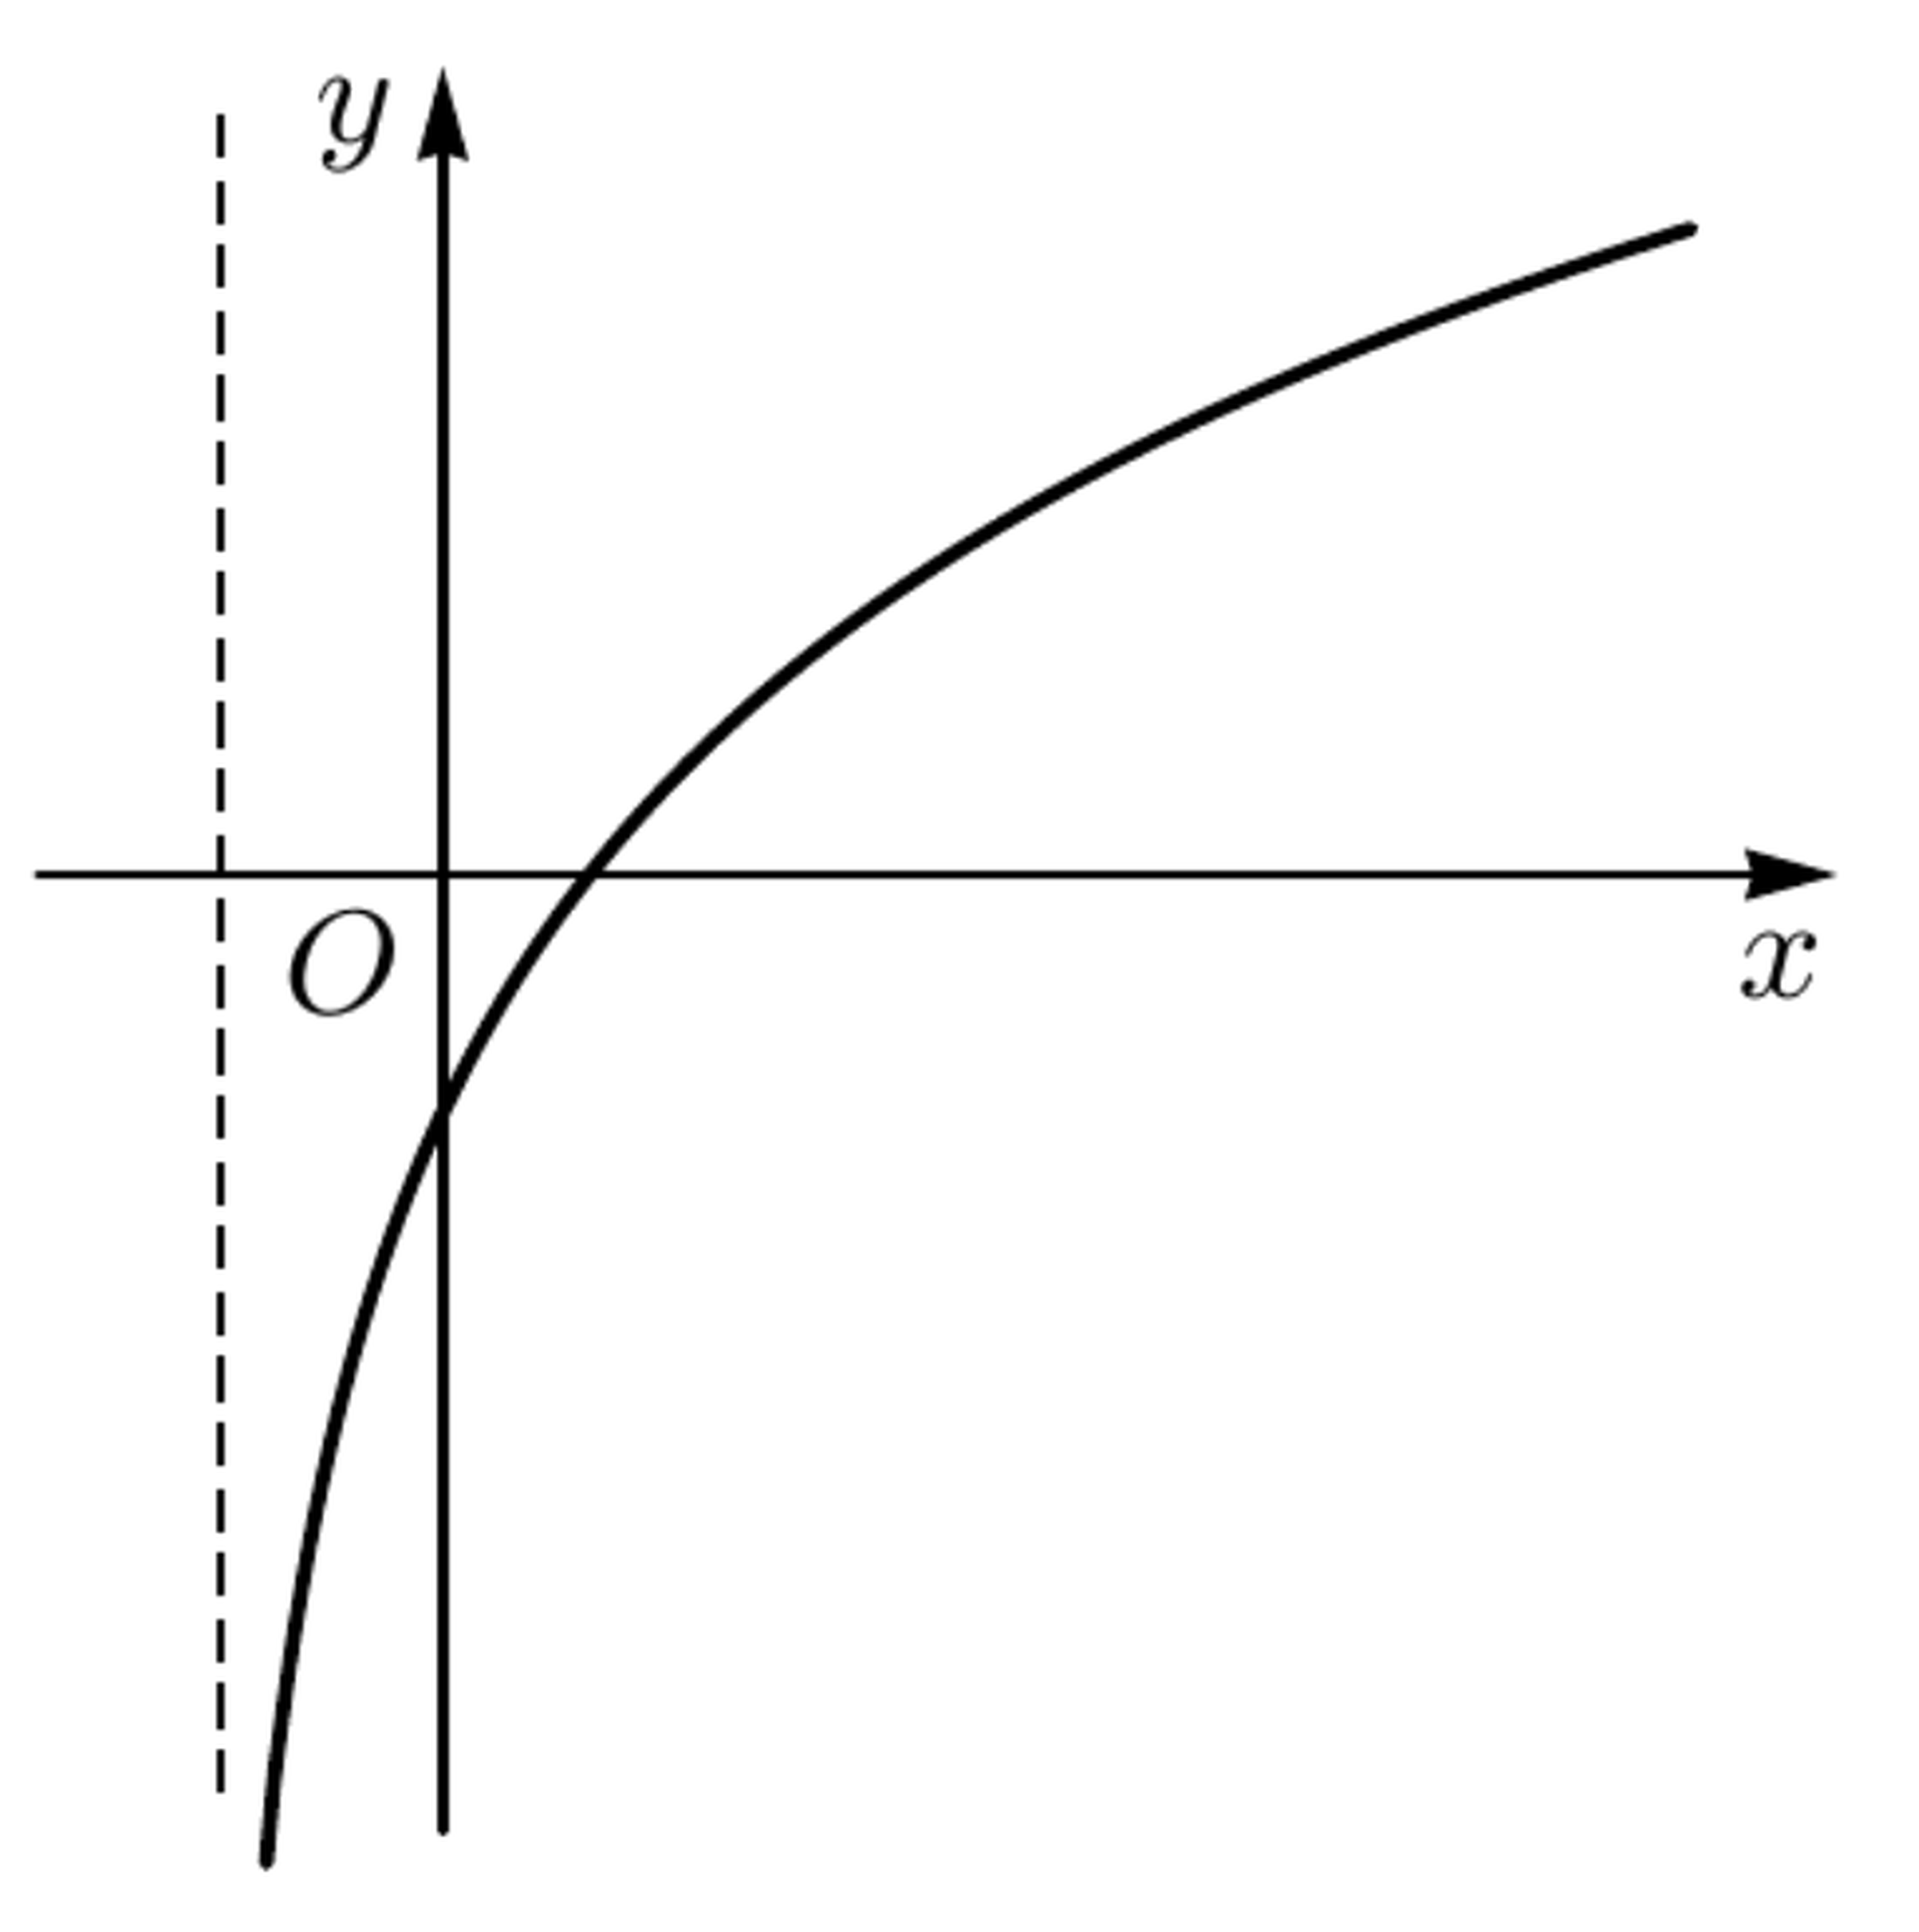
\includegraphics[width=0.42\textwidth]{figures/gao158_q15.png}
\end{center}

\keepwithprev
A. $a>1, b>1$\qquad\qquad B. $a>1, 0<b<1$

C. $0<a<1, b>1$\qquad\qquad D. $0<a<1, 0<b<1$

\ifanswer
\solbegin
\step{图像严格增，得 $a>1$.}
\step{图像与 $y$ 轴交于 $x$ 轴下方，得 $b>0$ 且 $\log_a b<0$，即 $0<b<1$，故选 $B$.}
\solend
\fi

% === Q16 === \lvert\log_2 x\rvert；解析 5 行，故选 C
\item 已知函数 $f(x)=\lvert\log_2 x\rvert$，若 $0<a<b$ 且 $f(a)=f(b)$，则 $a+2b$ 的取值范围是\mbox{（\quad）}

\keepwithprev
A. $(2\sqrt2,+\infty)$\qquad B. $[2\sqrt2,+\infty)$\qquad C. $(3,+\infty)$\qquad D. $[3,+\infty)$

\ifanswer
\solbegin
\step{由 $a<b$ 及 $\lvert\log_2 a\rvert=\lvert\log_2 b\rvert$，得 $\log_2 a=-\log_2 b$，即 $ab=1$，}
\step{且 $0<a<1<b$.}
\step{设 $t=a+2b=2b+\dfrac1b$，则 $t-3=\dfrac{(b-1)(2b-1)}{b}>0$.}
\step{反之，任取 $t>3$，令 $b=\dfrac{t+\sqrt{t^2-8}}{4}>1$、$a=\dfrac1b$，则满足题设且 $a+2b=t$.}
\step{因此取值范围为 $(3,+\infty)$，故选 $C$.}
\solend
\fi

\end{enumerate}

\bigsec{三、解答题}

\begin{enumerate}
\setcounter{enumi}{16}

% === Q17 === 集合、\overline{A}、\subseteq；解析 9 行
\item 已知全集 $U=\R$，集合 $A=\left\{x\mid\dfrac{x-3}{x+1}\leqslant0\right\}$，$B=\{x\mid x^2-2mx+m^2-9<0\}$（$m$ 为实数）.

(1) 当 $m=4$ 时，求 $A\cap B$ 和 $\overline{A}\cup B$；

(2) 若“$x\in A$”是“$x\in B$”的充分条件，求实数 $m$ 的取值范围.

\ifanswer
\solbegin
\step{(1) $\dfrac{x-3}{x+1}\leqslant0\Leftrightarrow-1<x\leqslant3$，所以 $A=(-1,3]$.}
\step{当 $m=4$ 时，$B=\{x\mid(x-4)^2<9\}=(1,7)$，}
\step{于是 $A\cap B=(1,3]$，$\overline{A}\cup B=(-\infty,-1]\cup(1,+\infty)$；}
\step{(2) $x^2-2mx+m^2-9<0\Leftrightarrow(x-m)^2<9$，所以 $B=(m-3,m+3)$.}
\step{题设充分条件等价于 $A\subseteq B$.}
\step{由于 $A=(-1,3]$，左端须满足 $m-3\leqslant-1$.}
\step{又 $3\in A$，须有 $3<m+3$.}
\step{这两个条件也保证 $(-1,3]\subseteq(m-3,m+3)$，}
\step{因此 $A\subseteq B\Leftrightarrow\begin{cases}m-3\leqslant-1\\m+3>3\end{cases}\Leftrightarrow0<m\leqslant2$.}
\solend
\fi

% === Q18 === 蓄水池造价（含 (3) 场地限制）；单位 \mathrm{m}；解析 13 行
\item 某工厂拟建一个容积为 $400\mathrm{m}^3$ 的无盖长方体蓄水池，池深 $4\mathrm{m}$，池底为矩形，其一边长
为 $x\mathrm{m}$. 池壁每平方米造价 100 元，池底每平方米造价 150 元. 设水池的总造价为 $C$
元.

(1) 把 $C$ 表示成 $x$ 的函数，并写出它的定义域；

(2) 当 $x$ 为何值时，总造价最低？最低造价是多少？

(3) 受场地限制，池底一边长 $x$ 不超过 $8\mathrm{m}$，此时总造价最低是多少？

\ifanswer
\solbegin
\step{(1) 设池底另一边长为 $y\mathrm{m}$，则 $4xy=400$，所以 $y=\dfrac{100}{x}$，$x>0$.}
\step{池底面积为 $100\mathrm{m}^2$，池壁总面积为 $8\left(x+\dfrac{100}{x}\right)\mathrm{m}^2$，}
\step{因此 $C(x)=100\times8\left(x+\dfrac{100}{x}\right)+150\times100=800x+\dfrac{80000}{x}+15000$，}
\step{定义域为 $(0,+\infty)$.}
\step{(2) 因为 $x>0$，所以 $C(x)=800\left(x+\dfrac{100}{x}\right)+15000$，}
\step{$\geqslant800\times2\sqrt{x\cdot\dfrac{100}{x}}+15000=31000$，}
\step{当且仅当 $x=\dfrac{100}{x}$，即 $x=10$ 时取等号.}
\step{答：当 $x=10$ 时，总造价最低，为 31000 元.}
\step{(3) 此时定义域为 $(0,8]$. 任取 $0<x_1<x_2\leqslant8$，}
\step{则 $C(x_2)-C(x_1)=800(x_2-x_1)\left(1-\dfrac{100}{x_1x_2}\right)<0$，}
\step{所以 $C(x)$ 在 $(0,8]$ 上严格递减，$x=8$ 时总造价最低，}
\step{且 $C(8)=800\times8+\dfrac{80000}{8}+15000=31400$.}
\step{答：受场地限制时，最低总造价为 31400 元.}
\solend
\fi

% === Q19 === 甲乙滤材 0.8^n／0.7^n；解析 17 行
\item 某环保公司研发了两种新型滤材甲和乙：污水每经过一层甲滤材，污染物含量减少
20\%；每经过一层乙滤材，污染物含量减少 30\%. 每层甲滤材成本 3 万元，每层乙滤材
成本 4 万元. 设原污水中污染物含量为 1，要求处理后污染物含量低于原来的 5\%.

(1) 若只使用一种滤材，污水经过 $n$ 层后污染物含量为 $y$，分别写出使用甲、乙两种滤材
时 $y$ 关于 $n$ 的函数关系式（$n$ 为正整数）；

(2) 若只使用一种滤材，分别求甲、乙至少各需要多少层，并比较哪种滤材的总成本更
低；

(3) 若两种滤材可以混合使用（先后顺序不影响效果），设使用甲滤材 $m$ 层、乙滤材 $n$
层（$m$、$n$ 为非负整数），求满足要求的最低总成本，并指出此时 $m$、$n$ 的值.

\ifanswer
\solbegin
\step{(1) 甲：$y=0.8^n$；乙：$y=0.7^n$，其中 $n$ 为正整数.}
\step{(2) 两种滤材均须满足 $y<0.05$，且污染物含量随层数增加而严格减少.}
\step{$0.8^{14}\approx0.04398<0.05<0.05498\approx0.8^{13}$，}
\step{$0.7^9=0.040353607<0.05<0.05764801=0.7^8$，}
\step{甲至少需要 14 层，成本为 $3\times14=42$ 万元；}
\step{乙至少需要 9 层，成本为 $4\times9=36$ 万元.}
\step{因此，只使用一种滤材时，使用乙滤材的总成本更低.}
\step{(3) 设总成本为 $C$ 万元，则 $C=3m+4n,0.8^m\cdot0.7^n<0.05,m,n\in\{0,1,2,\cdots\}$，}
\step{若 $m\geqslant3$，将其中 3 层甲替换为 2 层乙，}
\step{因为 $0.7^2=0.49<0.512=0.8^3,2\times4<3\times3$，}
\step{替换后污染物含量更低，成本减少 1 万元，因此最低成本方案必有 $m\leqslant2$.}
\step{当 $m=0$ 时，由第（2）小题得至少需要 9 层乙，最低成本为 36 万元.}
\step{当 $m=1$ 或 $m=2$ 时，$0.8\cdot0.7^7>0.8^2\cdot0.7^7=0.052706752>0.05$，}
\step{$0.8^2\cdot0.7^8<0.8\cdot0.7^8=0.046118408<0.05$，}
\step{因此两种情形均至少需要 8 层乙，}
\step{对应最低成本分别为 $3+4\times8=35$ 万元，$3\times2+4\times8=38$ 万元.}
\step{答：满足要求的最低总成本为 35 万元，此时使用甲滤材 1 层、乙滤材 8 层.}
\solend
\fi

% === Q20 === f(x)=\log_2(4^x+1)-x；\Delta；解析 17 行
\item 已知函数 $f(x)=\log_2(4^x+1)-x$.

(1) 证明 $f(x)=\log_2(2^x+2^{-x})$，并求 $f(x)$ 的最小值及取得最小值时 $x$ 的值；

(2) 解不等式 $f(x)>\log_2 5-1$；

(3) 证明：函数 $f(x)$ 在区间 $[0,+\infty)$ 上是严格增函数；并求使关于 $x$ 的方程 $f(x)=m$ 恰
有两个不同实数解的实数 $m$ 的取值范围.

\ifanswer
\solbegin
\step{(1) $f(x)=\log_2(4^x+1)-\log_2 2^x=\log_2\dfrac{4^x+1}{2^x}=\log_2(2^x+2^{-x})$，}
\step{因为 $2^x+2^{-x}\geqslant2\sqrt{2^x\cdot2^{-x}}=2$，所以 $f(x)\geqslant\log_2 2=1$，}
\step{等号当且仅当 $2^x=2^{-x}$，即 $x=0$ 时成立，故最小值为 1.}
\step{(2) 令 $t=2^x>0$，则 $f(x)>\log_2 5-1\Leftrightarrow t+\dfrac1t>\dfrac52\Leftrightarrow2t^2-5t+2>0$}
\step{$\Leftrightarrow(2t-1)(t-2)>0$，}
\step{结合 $t>0$，得 $0<t<\dfrac12$ 或 $t>2$，即 $x<-1$ 或 $x>1$，}
\step{解集为 $(-\infty,-1)\cup(1,+\infty)$.}
\step{(3) 任取 $0\leqslant x_1<x_2$，记 $a=2^{x_1}$，$b=2^{x_2}$，则 $1\leqslant a<b$，$ab>1$，}
\step{从而 $\left(b+\dfrac1b\right)-\left(a+\dfrac1a\right)=(b-a)\left(1-\dfrac{1}{ab}\right)>0$，}
\step{由对数函数的严格递增性，得 $f(x_1)<f(x_2)$，}
\step{所以 $f(x)$ 在 $[0,+\infty)$ 上是严格增函数.}
\step{当 $m<1$ 时，由（1）得方程无实数解；当 $m=1$ 时，只有实数解 $x=0$.}
\step{当 $m>1$ 时，令 $t=2^x>0$，则 $f(x)=m\Leftrightarrow t+\dfrac1t=2^m\Leftrightarrow t^2-2^m t+1=0$，}
\step{此时 $\Delta=2^{2m}-4>0$，两根之和为 $2^m>0$、之积为 $1>0$，}
\step{故有两个不同的正根.}
\step{每个正根 $t$ 唯一确定一个实数 $x=\log_2 t$，故原方程恰有两个不同实数解，}
\step{所求范围为 $m\in(1,+\infty)$.}
\solend
\fi

% === Q21 === f(x)=4^x-m\cdot2^{x+1}+3 值域与 h(m) 分段；解析 13 行
\item 已知函数 $f(x)=4^x-m\cdot2^{x+1}+3$（$m\in\R$），$x\in[0,2]$.

(1) 当 $m=1$ 时，求 $f(x)$ 的值域；

(2) 记 $f(x)$ 的最小值为 $h(m)$，求 $h(m)$ 的表达式；

(3) 若关于 $x$ 的方程 $f(x)=0$ 在区间 $[0,2]$ 上有解，求实数 $m$ 的取值范围.

\ifanswer
\solbegin
\step{令 $t=2^x$，则 $t\in[1,4]$，且 $f(x)=t^2-2mt+3=(t-m)^2+3-m^2$，}
\step{(1) 当 $m=1$ 时，$f(x)=(t-1)^2+2$.}
\step{由 $0\leqslant t-1\leqslant3$，得 $2\leqslant f(x)\leqslant11$，值域为 $[2,11]$.}
\step{(2) 二次函数 $y=(t-m)^2+3-m^2$ 的对称轴为直线 $t=m$.}
\step{当 $m\leqslant1$ 时，在 $t=1$ 处取最小值；}
\step{当 $1<m<4$ 时，在 $t=m$ 处取最小值；}
\step{当 $m\geqslant4$ 时，在 $t=4$ 处取最小值；}
\step{因此 $h(m)=\begin{cases}4-2m,&m\leqslant1\\3-m^2,&1<m<4\\19-8m,&m\geqslant4\end{cases}$；}
\step{(3) 方程 $f(x)=0$ 在 $[0,2]$ 上有解，}
\step{等价于存在 $t\in[1,4]$，使 $m=\dfrac{t^2+3}{2t}=\dfrac12\left(t+\dfrac3t\right)$，}
\step{由基本不等式，$m\geqslant\dfrac12\cdot2\sqrt{t\cdot\dfrac3t}=\sqrt3$，当且仅当 $t=\sqrt3$ 时取等号；}
\step{又 $\dfrac{19}{8}-m=\dfrac{(4-t)(4t-3)}{8t}\geqslant0$，当且仅当 $t=4$ 时取等号；}
\step{因此必有 $\sqrt3\leqslant m\leqslant\dfrac{19}{8}$.}
\solend
\fi

\end{enumerate}

\end{document}
"
% 紧凑版：xelatex "\def\iscompact{1}% 高一158_上实东滩_期中.tex
%   —— 高一上数学"2026-2027 年上实东滩高一上期中"（试卷版/答案版/紧凑版）
% 试卷版：xelatex 高一158_上实东滩_期中.tex
% 答案版：xelatex "\def\isanswer{1}\input{高一158_上实东滩_期中.tex}"
% 紧凑版：xelatex "\def\iscompact{1}\input{高一158_上实东滩_期中.tex}"
%
% ① 原始材料：微信公众号"魔都数学加油站"文章，连载"27学年高一158"，原文标题
% "27学年高一158——2026-2027年上海市上实东滩高一上期中"（本卷本地编号 158 与
% 原卷连载号一致，无撞号）。
% 正文为 9 张 PNG 页（01/05/08/09 为 2560×3620，02/03/04/06/07 为 4762×6735，
% 同一篇各页分辨率混排，逐页按各自分辨率裁图核对）。
% 体例：讲评版——填空 3—12（10 题）、选择 13—16（4 题）、解答 17—21（5 题），
% 共 19 题，自第 3 题起编（1、2 未印在本篇）；Q5 只印【答案】、其余 18 题
% 逐题印【解析】（逐题核实，见 ②）。题目、答案、解析均据原图转录；卷面粉红色
% 水印"魔都数学加油站"及公众号页脚未录入。全卷末题为第 21 题，无附加题节。
% 全卷 2 组配图（逐页通读 9 页确认）——
%   · Q10 题干右侧"曼 → man"字形变换图（02 页），题目配图、三版都出，
%     裁 figures/gao158_q10.png；
%   · Q15 题干"如图所示"对数函数大致图像（03 页右下），题目配图、三版都出，
%     裁 figures/gao158_q15.png；
% 2 图均取自原卷截图，去粉色水印、转灰度、4× LANCZOS 放大；
% 其余各页逐页确认无其它题目配图、无解析内配图、无表格。
%
% 卷首标题：原卷印作"2026-2027 年上实东滩高一上期中"，年份区间按全稿惯例排 en dash；
% 原卷卷面未印副标题，本稿按同期中卷知识模块口径补出"集合与常用逻辑用语、不等式、函数"。
%
% ② 与原卷的排版差异／照录项清单：
%   ① 原文从第 3 题起，本稿保留原题号；共 19 题三节，解答题 5 题到 21；
%      三节各自一个 enumerate＋各自 \setcounter{enumi}{2}／{12}／{16}，
%      不贯穿（题目溯源.py 按 \bigsec 切节、每节独立计 depth，只收 depth==1 的 \item）；
%   ② 混合体例：Q5 只印【答案】、无【解析】，按 高一156 第 3 题成例另提
%      \ans{}、不补造解析；其余 18 题印【解析】、用 \solbegin…\solend；
%      四道选择题答案均在解析末句"故选 C／B／B／C"（逐个放大复核）、
%      题干括号 \mbox{（\quad）} 留空、不另提 \ans{}；答案版
%      【答案】/【解析】标记数 = 19 = 全卷题数（1 个 \ans ＋ 18 个 \solbegin）；
%   ③ 原卷卷面未印副标题，本稿按知识模块口径补出；
%   ④ 原卷填空横线按全稿惯例排 \blankline[4.4em]；选择题选项段前按惯例各加
%      \keepwithprev；解答题不留作答区、不加 \anspace（原卷为讲评版）；
%   ⑤ 数集：Q13"在 \R 上严格递增"、Q14"$x\in\R$"、Q17"$U=\R$"、
%      Q21"$m\in\R$" 原卷印正体粗体 R，按全稿惯例归一 \R；
%      绝对值排 \lvert…\rvert（Q12 $\lvert a\rvert$、Q14 $\lvert x-2\rvert$、
%      Q16 $\lvert\log_2 x\rvert$／$\lvert\log_2 a\rvert$／$\lvert\log_2 b\rvert$），
%      集合描述竖线排 \mid（Q17），不等号按全稿惯例排 \leqslant／\geqslant，
%      补集上划线 \overline{A}（Q17）；
%   ⑥ 子集／真子集符号逐处照录不统一：Q14 解析"$(2,3)\subsetneq(1,3)$"原卷印
%      带下划线且被斜杠划过的 ⊊（真子集，放大 03 页确认），照录 \subsetneq；
%      Q17 解析三处"$A\subseteq B$""$(-1,3]\subseteq(m-3,m+3)$"原卷印
%      带下划线 ⊆（放大 05 页确认），照录 \subseteq；本卷无单线 \subset 用例；
%   ⑦ 判别式：Q20 (3) 解析"$\Delta=2^{2m}-4>0$"原卷印高瘦等腰 \Delta
%      （像素实测高/宽 ≈ 1.13，扁三角 \triangle 为 0.93，放大 08 页确认），
%      照录 \Delta；本卷无扁三角 \triangle 用例；
%   ⑧ "图像"与"图象"：全卷统一用"图像"（Q6 题干、Q10 两处、Q11 解析、
%      Q15 题干与解析两处，逐处放大确认带单人旁），照录不改；
%   ⑨ 中文弯引号照录：Q5 命题"若实数…"、Q10"曼""man""新"、Q14 题干与
%      解析的两则不等式、Q17 (2)"$x\in A$""$x\in B$"；注释里一律 ASCII 引号；
%   ⑩ 半角逗号逐处照录：Q8"$2,3,4$""$-2,-1,0$"、Q10 点坐标 $(x,y)$／
%      $(t,2^t-1)$／$(1-2^t,t)$、Q15 四选项"$a>1, b>1$"等、
%      Q19 (3)"$C=3m+4n,0.8^m\cdot0.7^n<0.05,m,n\in\{0,1,2,\cdots\}$"
%      与"$0.7^2=0.49<0.512=0.8^3,2\times4<3\times3$"、
%      Q21 cases 内"$4-2m,$"等；其余行中逗号／顿号照录全角；
%      行末西文句点 ASCII `.`；
%   ⑪ 顿号照录：Q3"（用 $a$、$b$ 表示）"、Q5"$x$、$y$"、Q13"A、B"、
%      Q16 解析"$>1$、$a=\dfrac1b$"、Q19"甲、乙""$m$、$n$"、
%      Q20"$2^m>0$、之积为"、Q21"$m$、$n$"；顿号一律移到数学模式外，
%      数学模式内不出现中文标点；
%   ⑫ 角度与单位照录：Q10 三处"$90^{\circ}$"、Q18"$400\mathrm{m}^3$"
%      "$4\mathrm{m}$""$x\mathrm{m}$""$8\mathrm{m}$""$y\mathrm{m}$"
%      "$100\mathrm{m}^2$""$\left(x+\dfrac{100}{x}\right)\mathrm{m}^2$"；
%      Q19 百分号"20\%""30\%""5\%"按原卷排 \%；
%   ⑬ 文本模式全角括号照录：Q10"（提示：…）"、Q17"（$m$ 为实数）"、
%      Q19"（$n$ 为正整数）""（先后顺序不影响效果）""（$m$、$n$ 为非负整数）"、
%      Q20"由（1）得"、Q19"由第（2）小题"、Q21"（$m\in\R$）"；
%      子题行首标号按全稿惯例用半角 (1)(2)(3)；
%   ⑭ 复杂式照录别简化：Q3 $\dfrac{\log_3 2+\log_3 5}{\log_3 3+2\log_3 2}$、
%      Q8 $[-3,-2)\cup(4,5]$、Q9 $18ab=2^t\cdot3^t=6^t=a+b$、
%      Q12 $\dfrac{\sqrt6}{2}$、Q18 $C(8)=800\times8+\dfrac{80000}{8}+15000=31400$
%      （原卷即 C(8)，非 C(2)）、Q19 $0.8^{14}\approx0.04398$、
%      $0.7^9=0.040353607$、$0.052706752$、$0.046118408$、
%      Q20 $t^2-2^m t+1=0$、Q21 $h(m)$ 三段 cases 与 $\dfrac{(4-t)(4t-3)}{8t}$ 等；
%      \left…\right 不得拆到不同 $…$ 组；cases 块整体算一个印刷行；
%   ⑮ 一条 \step = 原卷解析的一个印刷行；别并折行、别拆行。跨页续印按题合并
%      （Q7 的 01—02 页、Q9/Q10/Q11 的 02—03 页、Q13/Q14 的 03 页上下、
%      Q15/Q16 的 04 页上下、Q17 的 04—05 页、Q18 的 05—06 页、
%      Q19 的 06—07 页、Q20 的 07—08 页、Q21 的 08—09 页）；
%      跨半页重叠行（Q5【答案】、Q9 设公共值行、Q10 题干、Q16 反之行、
%      Q18 (2) 题干、Q19 末两行、Q20 (3) 末行、Q21 cases 块）只算一个印刷行；
%   ⑯ 配图：2 组题目配图（见 ①），均三版都出，\needvspace 守卫放 \item 之前
%      把"题干＋图"整块推走，\includegraphics 放题干之后；本卷无解析内配图、
%      无红字加粗小标题（全卷逐页确认，故无 \stepm）。
%
% ③ 行数复核：一条 \step = 原卷解析的一个印刷行，cases 块作一个印刷行计。
%   逐题数（逐页核对）：Q3：1；Q4：2；Q5：0（只印【答案】、提 \ans{}，
%   不计入 \step 账）；Q6：1；Q7：4；Q8：5；Q9：2；Q10：2；Q11：3；
%   Q12：3；Q13：2；Q14：3；Q15：2；Q16：5；Q17：9；Q18：13；
%   Q19：17；Q20：17；Q21：13。
%   合计 104 行（104 条 \step ＋ 0 条 \stepm），与原卷逐题印刷行相等。
%   全卷 19 题：Q5 一处 \ans{} ＋ 其余 18 题设 \solbegin…\solend，
%   答案版【答案】/【解析】标记数 = 19 = 全卷题数。
%
% ④ 页码分布（供回原图复核）：
%   卷首标题＋"一、填空题"＋Q3 题干＋解析 1 行、Q4 题干＋解析 2 行、
%   Q5 题干＋【答案】在 01 页上半；Q5【答案】（重叠重印）＋Q6 题干＋解析 1 行、
%   Q7 题干＋解析前 3 行在 01 页下半；Q7 解析末行＋Q8 题干＋解析 5 行、
%   Q9 题干＋解析首行在 02 页上半；Q9 解析末行＋Q10 题干（含"曼→man"图）
%   ＋解析 2 行＋Q11 题干＋解析首行在 02 页下半；Q11 解析后 2 行＋Q12 题干
%   ＋解析 3 行＋"二、选择题"标题＋Q13 题干＋选项在 03 页上半；
%   Q13 选项（重叠重印）＋解析 2 行＋Q14 题干＋选项＋解析 3 行＋Q15 题干
%   ＋对数图像（右侧）在 03 页下半；Q15 选项＋解析 2 行＋Q16 题干＋选项
%   ＋解析前 4 行在 04 页上半；Q16 解析末行＋"三、解答题"标题＋Q17 题干
%   ＋两问＋解析 (1) 3 行在 04 页下半；Q17 解析 (2) 6 行＋Q18 题干＋三问
%   ＋解析 (1) 4 行＋(2) 首行在 05 页上下；Q18 解析 (2) 后 3 行＋(3) 5 行
%   ＋Q19 题干＋三问＋解析 (1) 1 行＋(2) 3 行在 06 页上下；Q19 解析 (2) 3 行
%   ＋(3) 12 行在 07 页上半；Q19 解析末 2 行（重叠）＋Q20 题干＋三问
%   ＋解析 (1) 3 行在 07 页下半；Q20 解析 (2) 4 行＋(3) 前 4 行在 08 页上半；
%   Q20 解析 (3) 后 6 行＋Q21 题干＋(1) 问在 08 页下半；Q21 (2)(3) 问＋
%   解析 (1) 3 行＋(2) 5 行＋cases 块在 09 页上半；Q21 cases 块（重叠）
%   ＋(3) 解析 5 行在 09 页下半。本稿按题连排，不丢行、不并折行；
%   全卷末题为第 21 题，无附加题节。
%
% ⑤ 存疑／需主会话回原图复核：
%   1. Q14 解析"$(2,3)\subsetneq(1,3)$"的 ⊊（真子集带斜杠）与 Q17 的 ⊆
%      是两种不同记号，本稿分别照录 \subsetneq／\subseteq，请复核；
%   2. Q20 (3)"$\Delta=2^{2m}-4>0$"判为高瘦 \Delta，请复核是否 \triangle；
%   3. 任务书提示"Q18 解析里印 C(2)=…"，但 06 页原图逐处读作
%      $C(8)=800\times8+\dfrac{80000}{8}+15000=31400$，未找到 C(2)，
%      本稿照原卷排 C(8)，请复核；
%   4. Q19 解析末句"最低总成本为 35 万元"（07 页上下两处印同），
%      OCR 曾误读为 34，本稿按 35 照录，请复核；
%   5. Q10 提示末尾"坐标为 $(-y,x)$）."为半角 $)$＋全角 $）$ 两枚括号，
%      本稿照录，请复核；
%   6. Q21 cases 块后"；"落在分式中行右侧（排版居中基线所致），
%      本稿排作 $…\end{cases}$；，请复核。
%   全卷除此 6 类外未发现其它笔误／自相矛盾处；19 题中 18 题印【解析】。
%
\documentclass[a4paper,11pt]{article}
\usepackage{common}

\begin{document}

\examtitlest[3]{2026--2027 年上实东滩高一上期中}{集合与常用逻辑用语、不等式、函数}

\bigsec{一、填空题}

\begin{enumerate}
\setcounter{enumi}{2}

% === Q3 === 换底公式；解析 1 行
\item 已知 $3^a=5$，$\log_3 2=b$，则 $\log_{12} 10=$\blankline[4.4em]（用 $a$、$b$ 表示）.

\ifanswer
\solbegin
\step{$\log_{12} 10=\dfrac{\log_3 2+\log_3 5}{\log_3 3+2\log_3 2}=\dfrac{a+b}{1+2b}$.}
\solend
\fi

% === Q4 === 定义域；解析 2 行；半角括号 ( ) 与全角逗号照录
\item 函数 $y=\sqrt{2-x}+\lg(x^2-1)$ 的定义域为\blankline[4.4em].

\ifanswer
\solbegin
\step{由 $2-x\geqslant0$ 且 $x^2-1>0$，得 $x\leqslant2$ 且 ($x<-1$或$x>1$)，}
\step{定义域为 $(-\infty,-1)\cup(1,2]$.}
\solend
\fi

% === Q5 === 只印【答案】、无【解析】；反证法，中文弯引号
\item 用反证法证明命题“若实数 $x$、$y$ 满足 $x+y>2$，则 $x$、$y$ 中至少有一个大于 1”时，
应假设\blankline[4.4em].

\ifanswer
\ans{$x\leqslant1$ 且 $y\leqslant1$}
\fi

% === Q6 === 图像平移；解析 1 行
\item 函数 $y=\dfrac{2x+1}{x-1}$ 的图像可由函数 $y=\dfrac{3}{x}$ 的图像先向右平移 $a$ 个单位，再向上平移 $b$ 个单位
得到，则 $a+b=$\blankline[4.4em].

\ifanswer
\solbegin
\step{$y=\dfrac{2x+1}{x-1}=\dfrac{3}{x-1}+2$，所以 $a=1$，$b=2$，$a+b=3$.}
\solend
\fi

% === Q7 === 集合三元子集；解析 4 行，跨 01—02 页
\item 设 $A=\{a_1,a_2,a_3,a_4\}$ 是由四个实数组成的集合，若 $A$ 的所有三元子集中，三个元素之和
组成的集合为 $B=\{1,4,7,12\}$，则集合 $A=$\blankline[4.4em].

\ifanswer
\solbegin
\step{设 $S=a_1+a_2+a_3+a_4$，}
\step{每个元素在四个三元子集中恰出现三次，则 $3S=1+4+7+12=24$，得 $S=8$.}
\step{四个三元子集的元素和分别为 $S-a_i$，}
\step{所以 $A=\{8-1,8-4,8-7,8-12\}=\{-4,1,4,7\}$.}
\solend
\fi

% === Q8 === 不等式整数解；解析 5 行；半角逗号照录
\item 不等式 $x^2-(a+1)x+a<0$ 的解集中恰有 3 个整数，则 $a$ 的取值范围是\blankline[4.4em].

\ifanswer
\solbegin
\step{原不等式为 $(x-1)(x-a)<0$；}
\step{$a=1$ 时解集为空集，不符合题意.}
\step{若 $a>1$，解集为 $(1,a)$，恰含整数 $2,3,4$，则 $4<a\leqslant5$.}
\step{若 $a<1$，解集为 $(a,1)$，恰含整数 $-2,-1,0$，则 $-3\leqslant a<-2$.}
\step{故 $a$ 的取值范围是 $[-3,-2)\cup(4,5]$.}
\solend
\fi

% === Q9 === 对数换底＋指数；解析 2 行
\item 已知正数 $a$、$b$ 满足 $1+\log_2 a=2+\log_3 b=\log_6(a+b)$，则 $\dfrac1a+\dfrac1b=$\blankline[4.4em].

\ifanswer
\solbegin
\step{设公共值为 $t$，则 $2a=2^t$，$9b=3^t$，$a+b=6^t$，}
\step{于是 $18ab=2^t\cdot3^t=6^t=a+b$，即 $\dfrac1a+\dfrac1b=\dfrac{a+b}{ab}=18$.}
\solend
\fi

% === Q10 === "曼"字旋转 90°；题目配图（三版都出）；解析 2 行
\needvspace{6cm}
\item 网上流传一个有趣的字形变换：把汉字“曼”的右半部分旋转 $90^{\circ}$，就得到英文单词
“man”的艺术字. 数学中，把曲线绕原点旋转也会得到“新”的曲线：将函数
$y=2^x-1$ 的图像绕坐标原点 $O$ 逆时针旋转 $90^{\circ}$，得到的曲线恰是某个函数的
图像，则这个函数的解析式为\blankline[4.4em]（提示：点 $(x,y)$ 绕 $O$ 逆时针旋转 $90^{\circ}$ 后的
坐标为 $(-y,x)$）.

\begin{center}

\includegraphics[width=0.42\textwidth]{figures/gao158_q10.png}
\end{center}

\ifanswer
\solbegin
\step{原图像上的点 $(t,2^t-1)$ 旋转后为 $(1-2^t,t)$.}
\step{记其为 $(x,y)$，则 $x=1-2^y$，即 $y=\log_2(1-x)$，定义域为 $(-\infty,1)$.}
\solend
\fi

% === Q11 === 值域；解析 3 行，跨 02—03 页
\item 函数 $f(x)=\sqrt{x-2}-\sqrt{15-3x}$ 的值域为\blankline[4.4em].

\ifanswer
\solbegin
\step{由 $x-2\geqslant0$ 且 $15-3x\geqslant0$，得定义域为 $[2,5]$.}
\step{在 $[2,5]$ 上，$\sqrt{x-2}$ 与 $-\sqrt{15-3x}$ 均严格递增，因此 $f(x)$ 严格递增.}
\step{$f(2)=-3$，$f(5)=\sqrt3$，结合函数的图像，值域为 $[-3,\sqrt3]$.}
\solend
\fi

% === Q12 === 绝对值 \lvert…\rvert；解析 3 行
\item 设实数 $a$ 满足 $a<4a^3-5a<\lvert a\rvert$，则 $a$ 的取值范围是\blankline[4.4em].

\ifanswer
\solbegin
\step{由 $a<\lvert a\rvert$ 得 $a<0$，原不等式为 $a<4a^3-5a<-a$.}
\step{同除以 $a<0$，得 $1>4a^2-5>-1\Leftrightarrow1<a^2<\dfrac32$，结合 $a<0$，}
\step{得 $-\dfrac{\sqrt6}{2}<a<-1$，故解集为 $\left(-\dfrac{\sqrt6}{2},-1\right)$.}
\solend
\fi

\end{enumerate}

\bigsec{二、选择题}

\begin{enumerate}
\setcounter{enumi}{12}

% === Q13 === \R 归一；解析 2 行，故选 C
\item 已知 $a>b$，则下列不等式一定成立的是\mbox{（\quad）}

\keepwithprev
A. $\dfrac1a<\dfrac1b$\qquad B. $a^2>b^2$\qquad C. $a^3>b^3$\qquad D. $ac^2>bc^2$

\ifanswer
\solbegin
\step{幂函数 $y=x^3$ 在 $\R$ 上严格递增，$a>b\Rightarrow a^3>b^3$，C 正确.}
\step{取 $a=1$，$b=-1$ 得 A、B 不成立；取 $c=0$ 得 D 不成立；故选 $C$.}
\solend
\fi

% === Q14 === \subsetneq 真子集；解析 3 行，故选 B
\item 设 $x\in\R$，则“$\lvert x-2\rvert<1$”是“$x^2-5x+6<0$”的\mbox{（\quad）}

\keepwithprev
A. 充分非必要条件\qquad\qquad B. 必要非充分条件

C. 充要条件\qquad\qquad D. 既非充分又非必要条件

\ifanswer
\solbegin
\step{$\lvert x-2\rvert<1\Leftrightarrow1<x<3$，$x^2-5x+6<0\Leftrightarrow(x-2)(x-3)<0\Leftrightarrow2<x<3$.}
\step{由 $(2,3)\subsetneq(1,3)$，得“$\lvert x-2\rvert<1$”是“$x^2-5x+6<0$”的必要非充分条件，}
\step{故选 $B$.}
\solend
\fi

% === Q15 === 对数函数大致图像（题目配图，三版都出）；解析 2 行，故选 B
\needvspace{9cm}
\item 已知函数 $f(x)=\log_a(x+b)$（$a>0$ 且 $a\ne1$）的大致图像如图所示，则 $a$、$b$ 满足
的关系是\mbox{（\quad）}

\begin{center}
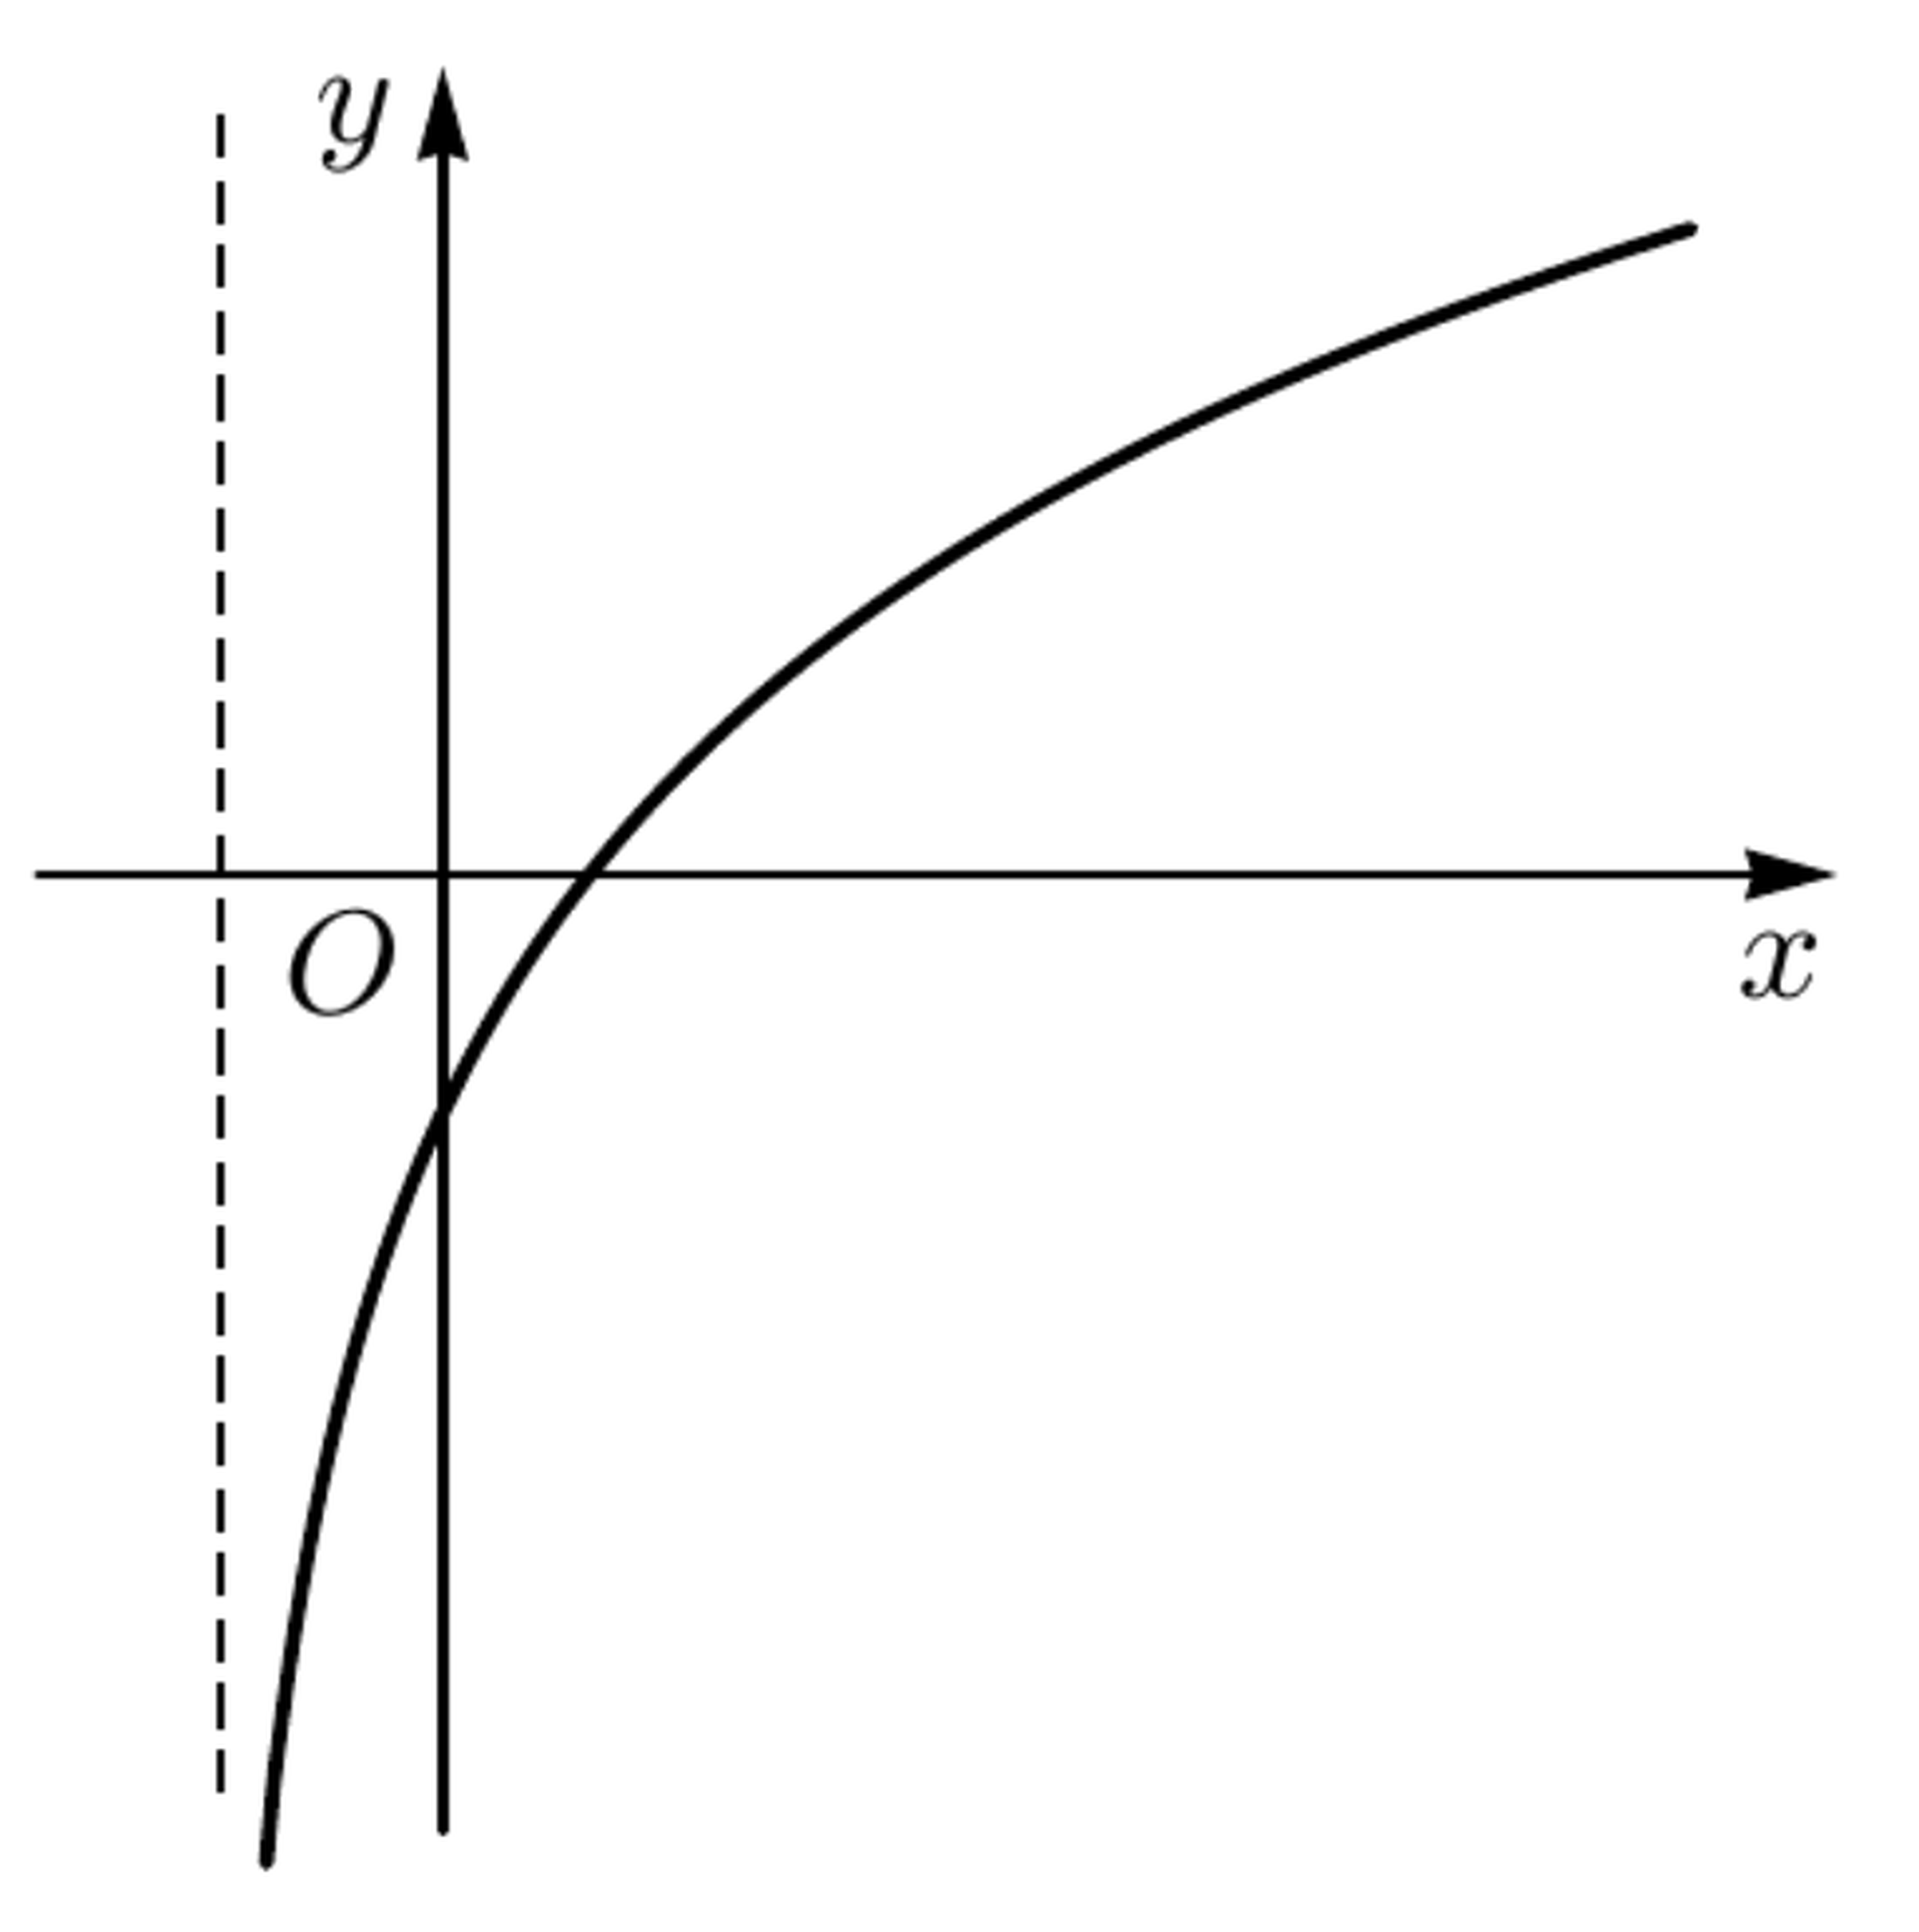
\includegraphics[width=0.42\textwidth]{figures/gao158_q15.png}
\end{center}

\keepwithprev
A. $a>1, b>1$\qquad\qquad B. $a>1, 0<b<1$

C. $0<a<1, b>1$\qquad\qquad D. $0<a<1, 0<b<1$

\ifanswer
\solbegin
\step{图像严格增，得 $a>1$.}
\step{图像与 $y$ 轴交于 $x$ 轴下方，得 $b>0$ 且 $\log_a b<0$，即 $0<b<1$，故选 $B$.}
\solend
\fi

% === Q16 === \lvert\log_2 x\rvert；解析 5 行，故选 C
\item 已知函数 $f(x)=\lvert\log_2 x\rvert$，若 $0<a<b$ 且 $f(a)=f(b)$，则 $a+2b$ 的取值范围是\mbox{（\quad）}

\keepwithprev
A. $(2\sqrt2,+\infty)$\qquad B. $[2\sqrt2,+\infty)$\qquad C. $(3,+\infty)$\qquad D. $[3,+\infty)$

\ifanswer
\solbegin
\step{由 $a<b$ 及 $\lvert\log_2 a\rvert=\lvert\log_2 b\rvert$，得 $\log_2 a=-\log_2 b$，即 $ab=1$，}
\step{且 $0<a<1<b$.}
\step{设 $t=a+2b=2b+\dfrac1b$，则 $t-3=\dfrac{(b-1)(2b-1)}{b}>0$.}
\step{反之，任取 $t>3$，令 $b=\dfrac{t+\sqrt{t^2-8}}{4}>1$、$a=\dfrac1b$，则满足题设且 $a+2b=t$.}
\step{因此取值范围为 $(3,+\infty)$，故选 $C$.}
\solend
\fi

\end{enumerate}

\bigsec{三、解答题}

\begin{enumerate}
\setcounter{enumi}{16}

% === Q17 === 集合、\overline{A}、\subseteq；解析 9 行
\item 已知全集 $U=\R$，集合 $A=\left\{x\mid\dfrac{x-3}{x+1}\leqslant0\right\}$，$B=\{x\mid x^2-2mx+m^2-9<0\}$（$m$ 为实数）.

(1) 当 $m=4$ 时，求 $A\cap B$ 和 $\overline{A}\cup B$；

(2) 若“$x\in A$”是“$x\in B$”的充分条件，求实数 $m$ 的取值范围.

\ifanswer
\solbegin
\step{(1) $\dfrac{x-3}{x+1}\leqslant0\Leftrightarrow-1<x\leqslant3$，所以 $A=(-1,3]$.}
\step{当 $m=4$ 时，$B=\{x\mid(x-4)^2<9\}=(1,7)$，}
\step{于是 $A\cap B=(1,3]$，$\overline{A}\cup B=(-\infty,-1]\cup(1,+\infty)$；}
\step{(2) $x^2-2mx+m^2-9<0\Leftrightarrow(x-m)^2<9$，所以 $B=(m-3,m+3)$.}
\step{题设充分条件等价于 $A\subseteq B$.}
\step{由于 $A=(-1,3]$，左端须满足 $m-3\leqslant-1$.}
\step{又 $3\in A$，须有 $3<m+3$.}
\step{这两个条件也保证 $(-1,3]\subseteq(m-3,m+3)$，}
\step{因此 $A\subseteq B\Leftrightarrow\begin{cases}m-3\leqslant-1\\m+3>3\end{cases}\Leftrightarrow0<m\leqslant2$.}
\solend
\fi

% === Q18 === 蓄水池造价（含 (3) 场地限制）；单位 \mathrm{m}；解析 13 行
\item 某工厂拟建一个容积为 $400\mathrm{m}^3$ 的无盖长方体蓄水池，池深 $4\mathrm{m}$，池底为矩形，其一边长
为 $x\mathrm{m}$. 池壁每平方米造价 100 元，池底每平方米造价 150 元. 设水池的总造价为 $C$
元.

(1) 把 $C$ 表示成 $x$ 的函数，并写出它的定义域；

(2) 当 $x$ 为何值时，总造价最低？最低造价是多少？

(3) 受场地限制，池底一边长 $x$ 不超过 $8\mathrm{m}$，此时总造价最低是多少？

\ifanswer
\solbegin
\step{(1) 设池底另一边长为 $y\mathrm{m}$，则 $4xy=400$，所以 $y=\dfrac{100}{x}$，$x>0$.}
\step{池底面积为 $100\mathrm{m}^2$，池壁总面积为 $8\left(x+\dfrac{100}{x}\right)\mathrm{m}^2$，}
\step{因此 $C(x)=100\times8\left(x+\dfrac{100}{x}\right)+150\times100=800x+\dfrac{80000}{x}+15000$，}
\step{定义域为 $(0,+\infty)$.}
\step{(2) 因为 $x>0$，所以 $C(x)=800\left(x+\dfrac{100}{x}\right)+15000$，}
\step{$\geqslant800\times2\sqrt{x\cdot\dfrac{100}{x}}+15000=31000$，}
\step{当且仅当 $x=\dfrac{100}{x}$，即 $x=10$ 时取等号.}
\step{答：当 $x=10$ 时，总造价最低，为 31000 元.}
\step{(3) 此时定义域为 $(0,8]$. 任取 $0<x_1<x_2\leqslant8$，}
\step{则 $C(x_2)-C(x_1)=800(x_2-x_1)\left(1-\dfrac{100}{x_1x_2}\right)<0$，}
\step{所以 $C(x)$ 在 $(0,8]$ 上严格递减，$x=8$ 时总造价最低，}
\step{且 $C(8)=800\times8+\dfrac{80000}{8}+15000=31400$.}
\step{答：受场地限制时，最低总造价为 31400 元.}
\solend
\fi

% === Q19 === 甲乙滤材 0.8^n／0.7^n；解析 17 行
\item 某环保公司研发了两种新型滤材甲和乙：污水每经过一层甲滤材，污染物含量减少
20\%；每经过一层乙滤材，污染物含量减少 30\%. 每层甲滤材成本 3 万元，每层乙滤材
成本 4 万元. 设原污水中污染物含量为 1，要求处理后污染物含量低于原来的 5\%.

(1) 若只使用一种滤材，污水经过 $n$ 层后污染物含量为 $y$，分别写出使用甲、乙两种滤材
时 $y$ 关于 $n$ 的函数关系式（$n$ 为正整数）；

(2) 若只使用一种滤材，分别求甲、乙至少各需要多少层，并比较哪种滤材的总成本更
低；

(3) 若两种滤材可以混合使用（先后顺序不影响效果），设使用甲滤材 $m$ 层、乙滤材 $n$
层（$m$、$n$ 为非负整数），求满足要求的最低总成本，并指出此时 $m$、$n$ 的值.

\ifanswer
\solbegin
\step{(1) 甲：$y=0.8^n$；乙：$y=0.7^n$，其中 $n$ 为正整数.}
\step{(2) 两种滤材均须满足 $y<0.05$，且污染物含量随层数增加而严格减少.}
\step{$0.8^{14}\approx0.04398<0.05<0.05498\approx0.8^{13}$，}
\step{$0.7^9=0.040353607<0.05<0.05764801=0.7^8$，}
\step{甲至少需要 14 层，成本为 $3\times14=42$ 万元；}
\step{乙至少需要 9 层，成本为 $4\times9=36$ 万元.}
\step{因此，只使用一种滤材时，使用乙滤材的总成本更低.}
\step{(3) 设总成本为 $C$ 万元，则 $C=3m+4n,0.8^m\cdot0.7^n<0.05,m,n\in\{0,1,2,\cdots\}$，}
\step{若 $m\geqslant3$，将其中 3 层甲替换为 2 层乙，}
\step{因为 $0.7^2=0.49<0.512=0.8^3,2\times4<3\times3$，}
\step{替换后污染物含量更低，成本减少 1 万元，因此最低成本方案必有 $m\leqslant2$.}
\step{当 $m=0$ 时，由第（2）小题得至少需要 9 层乙，最低成本为 36 万元.}
\step{当 $m=1$ 或 $m=2$ 时，$0.8\cdot0.7^7>0.8^2\cdot0.7^7=0.052706752>0.05$，}
\step{$0.8^2\cdot0.7^8<0.8\cdot0.7^8=0.046118408<0.05$，}
\step{因此两种情形均至少需要 8 层乙，}
\step{对应最低成本分别为 $3+4\times8=35$ 万元，$3\times2+4\times8=38$ 万元.}
\step{答：满足要求的最低总成本为 35 万元，此时使用甲滤材 1 层、乙滤材 8 层.}
\solend
\fi

% === Q20 === f(x)=\log_2(4^x+1)-x；\Delta；解析 17 行
\item 已知函数 $f(x)=\log_2(4^x+1)-x$.

(1) 证明 $f(x)=\log_2(2^x+2^{-x})$，并求 $f(x)$ 的最小值及取得最小值时 $x$ 的值；

(2) 解不等式 $f(x)>\log_2 5-1$；

(3) 证明：函数 $f(x)$ 在区间 $[0,+\infty)$ 上是严格增函数；并求使关于 $x$ 的方程 $f(x)=m$ 恰
有两个不同实数解的实数 $m$ 的取值范围.

\ifanswer
\solbegin
\step{(1) $f(x)=\log_2(4^x+1)-\log_2 2^x=\log_2\dfrac{4^x+1}{2^x}=\log_2(2^x+2^{-x})$，}
\step{因为 $2^x+2^{-x}\geqslant2\sqrt{2^x\cdot2^{-x}}=2$，所以 $f(x)\geqslant\log_2 2=1$，}
\step{等号当且仅当 $2^x=2^{-x}$，即 $x=0$ 时成立，故最小值为 1.}
\step{(2) 令 $t=2^x>0$，则 $f(x)>\log_2 5-1\Leftrightarrow t+\dfrac1t>\dfrac52\Leftrightarrow2t^2-5t+2>0$}
\step{$\Leftrightarrow(2t-1)(t-2)>0$，}
\step{结合 $t>0$，得 $0<t<\dfrac12$ 或 $t>2$，即 $x<-1$ 或 $x>1$，}
\step{解集为 $(-\infty,-1)\cup(1,+\infty)$.}
\step{(3) 任取 $0\leqslant x_1<x_2$，记 $a=2^{x_1}$，$b=2^{x_2}$，则 $1\leqslant a<b$，$ab>1$，}
\step{从而 $\left(b+\dfrac1b\right)-\left(a+\dfrac1a\right)=(b-a)\left(1-\dfrac{1}{ab}\right)>0$，}
\step{由对数函数的严格递增性，得 $f(x_1)<f(x_2)$，}
\step{所以 $f(x)$ 在 $[0,+\infty)$ 上是严格增函数.}
\step{当 $m<1$ 时，由（1）得方程无实数解；当 $m=1$ 时，只有实数解 $x=0$.}
\step{当 $m>1$ 时，令 $t=2^x>0$，则 $f(x)=m\Leftrightarrow t+\dfrac1t=2^m\Leftrightarrow t^2-2^m t+1=0$，}
\step{此时 $\Delta=2^{2m}-4>0$，两根之和为 $2^m>0$、之积为 $1>0$，}
\step{故有两个不同的正根.}
\step{每个正根 $t$ 唯一确定一个实数 $x=\log_2 t$，故原方程恰有两个不同实数解，}
\step{所求范围为 $m\in(1,+\infty)$.}
\solend
\fi

% === Q21 === f(x)=4^x-m\cdot2^{x+1}+3 值域与 h(m) 分段；解析 13 行
\item 已知函数 $f(x)=4^x-m\cdot2^{x+1}+3$（$m\in\R$），$x\in[0,2]$.

(1) 当 $m=1$ 时，求 $f(x)$ 的值域；

(2) 记 $f(x)$ 的最小值为 $h(m)$，求 $h(m)$ 的表达式；

(3) 若关于 $x$ 的方程 $f(x)=0$ 在区间 $[0,2]$ 上有解，求实数 $m$ 的取值范围.

\ifanswer
\solbegin
\step{令 $t=2^x$，则 $t\in[1,4]$，且 $f(x)=t^2-2mt+3=(t-m)^2+3-m^2$，}
\step{(1) 当 $m=1$ 时，$f(x)=(t-1)^2+2$.}
\step{由 $0\leqslant t-1\leqslant3$，得 $2\leqslant f(x)\leqslant11$，值域为 $[2,11]$.}
\step{(2) 二次函数 $y=(t-m)^2+3-m^2$ 的对称轴为直线 $t=m$.}
\step{当 $m\leqslant1$ 时，在 $t=1$ 处取最小值；}
\step{当 $1<m<4$ 时，在 $t=m$ 处取最小值；}
\step{当 $m\geqslant4$ 时，在 $t=4$ 处取最小值；}
\step{因此 $h(m)=\begin{cases}4-2m,&m\leqslant1\\3-m^2,&1<m<4\\19-8m,&m\geqslant4\end{cases}$；}
\step{(3) 方程 $f(x)=0$ 在 $[0,2]$ 上有解，}
\step{等价于存在 $t\in[1,4]$，使 $m=\dfrac{t^2+3}{2t}=\dfrac12\left(t+\dfrac3t\right)$，}
\step{由基本不等式，$m\geqslant\dfrac12\cdot2\sqrt{t\cdot\dfrac3t}=\sqrt3$，当且仅当 $t=\sqrt3$ 时取等号；}
\step{又 $\dfrac{19}{8}-m=\dfrac{(4-t)(4t-3)}{8t}\geqslant0$，当且仅当 $t=4$ 时取等号；}
\step{因此必有 $\sqrt3\leqslant m\leqslant\dfrac{19}{8}$.}
\solend
\fi

\end{enumerate}

\end{document}
"
%
% ① 原始材料：微信公众号"魔都数学加油站"文章，连载"27学年高一158"，原文标题
% "27学年高一158——2026-2027年上海市上实东滩高一上期中"（本卷本地编号 158 与
% 原卷连载号一致，无撞号）。
% 正文为 9 张 PNG 页（01/05/08/09 为 2560×3620，02/03/04/06/07 为 4762×6735，
% 同一篇各页分辨率混排，逐页按各自分辨率裁图核对）。
% 体例：讲评版——填空 3—12（10 题）、选择 13—16（4 题）、解答 17—21（5 题），
% 共 19 题，自第 3 题起编（1、2 未印在本篇）；Q5 只印【答案】、其余 18 题
% 逐题印【解析】（逐题核实，见 ②）。题目、答案、解析均据原图转录；卷面粉红色
% 水印"魔都数学加油站"及公众号页脚未录入。全卷末题为第 21 题，无附加题节。
% 全卷 2 组配图（逐页通读 9 页确认）——
%   · Q10 题干右侧"曼 → man"字形变换图（02 页），题目配图、三版都出，
%     裁 figures/gao158_q10.png；
%   · Q15 题干"如图所示"对数函数大致图像（03 页右下），题目配图、三版都出，
%     裁 figures/gao158_q15.png；
% 2 图均取自原卷截图，去粉色水印、转灰度、4× LANCZOS 放大；
% 其余各页逐页确认无其它题目配图、无解析内配图、无表格。
%
% 卷首标题：原卷印作"2026-2027 年上实东滩高一上期中"，年份区间按全稿惯例排 en dash；
% 原卷卷面未印副标题，本稿按同期中卷知识模块口径补出"集合与常用逻辑用语、不等式、函数"。
%
% ② 与原卷的排版差异／照录项清单：
%   ① 原文从第 3 题起，本稿保留原题号；共 19 题三节，解答题 5 题到 21；
%      三节各自一个 enumerate＋各自 \setcounter{enumi}{2}／{12}／{16}，
%      不贯穿（题目溯源.py 按 \bigsec 切节、每节独立计 depth，只收 depth==1 的 \item）；
%   ② 混合体例：Q5 只印【答案】、无【解析】，按 高一156 第 3 题成例另提
%      \ans{}、不补造解析；其余 18 题印【解析】、用 \solbegin…\solend；
%      四道选择题答案均在解析末句"故选 C／B／B／C"（逐个放大复核）、
%      题干括号 \mbox{（\quad）} 留空、不另提 \ans{}；答案版
%      【答案】/【解析】标记数 = 19 = 全卷题数（1 个 \ans ＋ 18 个 \solbegin）；
%   ③ 原卷卷面未印副标题，本稿按知识模块口径补出；
%   ④ 原卷填空横线按全稿惯例排 \blankline[4.4em]；选择题选项段前按惯例各加
%      \keepwithprev；解答题不留作答区、不加 \anspace（原卷为讲评版）；
%   ⑤ 数集：Q13"在 \R 上严格递增"、Q14"$x\in\R$"、Q17"$U=\R$"、
%      Q21"$m\in\R$" 原卷印正体粗体 R，按全稿惯例归一 \R；
%      绝对值排 \lvert…\rvert（Q12 $\lvert a\rvert$、Q14 $\lvert x-2\rvert$、
%      Q16 $\lvert\log_2 x\rvert$／$\lvert\log_2 a\rvert$／$\lvert\log_2 b\rvert$），
%      集合描述竖线排 \mid（Q17），不等号按全稿惯例排 \leqslant／\geqslant，
%      补集上划线 \overline{A}（Q17）；
%   ⑥ 子集／真子集符号逐处照录不统一：Q14 解析"$(2,3)\subsetneq(1,3)$"原卷印
%      带下划线且被斜杠划过的 ⊊（真子集，放大 03 页确认），照录 \subsetneq；
%      Q17 解析三处"$A\subseteq B$""$(-1,3]\subseteq(m-3,m+3)$"原卷印
%      带下划线 ⊆（放大 05 页确认），照录 \subseteq；本卷无单线 \subset 用例；
%   ⑦ 判别式：Q20 (3) 解析"$\Delta=2^{2m}-4>0$"原卷印高瘦等腰 \Delta
%      （像素实测高/宽 ≈ 1.13，扁三角 \triangle 为 0.93，放大 08 页确认），
%      照录 \Delta；本卷无扁三角 \triangle 用例；
%   ⑧ "图像"与"图象"：全卷统一用"图像"（Q6 题干、Q10 两处、Q11 解析、
%      Q15 题干与解析两处，逐处放大确认带单人旁），照录不改；
%   ⑨ 中文弯引号照录：Q5 命题"若实数…"、Q10"曼""man""新"、Q14 题干与
%      解析的两则不等式、Q17 (2)"$x\in A$""$x\in B$"；注释里一律 ASCII 引号；
%   ⑩ 半角逗号逐处照录：Q8"$2,3,4$""$-2,-1,0$"、Q10 点坐标 $(x,y)$／
%      $(t,2^t-1)$／$(1-2^t,t)$、Q15 四选项"$a>1, b>1$"等、
%      Q19 (3)"$C=3m+4n,0.8^m\cdot0.7^n<0.05,m,n\in\{0,1,2,\cdots\}$"
%      与"$0.7^2=0.49<0.512=0.8^3,2\times4<3\times3$"、
%      Q21 cases 内"$4-2m,$"等；其余行中逗号／顿号照录全角；
%      行末西文句点 ASCII `.`；
%   ⑪ 顿号照录：Q3"（用 $a$、$b$ 表示）"、Q5"$x$、$y$"、Q13"A、B"、
%      Q16 解析"$>1$、$a=\dfrac1b$"、Q19"甲、乙""$m$、$n$"、
%      Q20"$2^m>0$、之积为"、Q21"$m$、$n$"；顿号一律移到数学模式外，
%      数学模式内不出现中文标点；
%   ⑫ 角度与单位照录：Q10 三处"$90^{\circ}$"、Q18"$400\mathrm{m}^3$"
%      "$4\mathrm{m}$""$x\mathrm{m}$""$8\mathrm{m}$""$y\mathrm{m}$"
%      "$100\mathrm{m}^2$""$\left(x+\dfrac{100}{x}\right)\mathrm{m}^2$"；
%      Q19 百分号"20\%""30\%""5\%"按原卷排 \%；
%   ⑬ 文本模式全角括号照录：Q10"（提示：…）"、Q17"（$m$ 为实数）"、
%      Q19"（$n$ 为正整数）""（先后顺序不影响效果）""（$m$、$n$ 为非负整数）"、
%      Q20"由（1）得"、Q19"由第（2）小题"、Q21"（$m\in\R$）"；
%      子题行首标号按全稿惯例用半角 (1)(2)(3)；
%   ⑭ 复杂式照录别简化：Q3 $\dfrac{\log_3 2+\log_3 5}{\log_3 3+2\log_3 2}$、
%      Q8 $[-3,-2)\cup(4,5]$、Q9 $18ab=2^t\cdot3^t=6^t=a+b$、
%      Q12 $\dfrac{\sqrt6}{2}$、Q18 $C(8)=800\times8+\dfrac{80000}{8}+15000=31400$
%      （原卷即 C(8)，非 C(2)）、Q19 $0.8^{14}\approx0.04398$、
%      $0.7^9=0.040353607$、$0.052706752$、$0.046118408$、
%      Q20 $t^2-2^m t+1=0$、Q21 $h(m)$ 三段 cases 与 $\dfrac{(4-t)(4t-3)}{8t}$ 等；
%      \left…\right 不得拆到不同 $…$ 组；cases 块整体算一个印刷行；
%   ⑮ 一条 \step = 原卷解析的一个印刷行；别并折行、别拆行。跨页续印按题合并
%      （Q7 的 01—02 页、Q9/Q10/Q11 的 02—03 页、Q13/Q14 的 03 页上下、
%      Q15/Q16 的 04 页上下、Q17 的 04—05 页、Q18 的 05—06 页、
%      Q19 的 06—07 页、Q20 的 07—08 页、Q21 的 08—09 页）；
%      跨半页重叠行（Q5【答案】、Q9 设公共值行、Q10 题干、Q16 反之行、
%      Q18 (2) 题干、Q19 末两行、Q20 (3) 末行、Q21 cases 块）只算一个印刷行；
%   ⑯ 配图：2 组题目配图（见 ①），均三版都出，\needvspace 守卫放 \item 之前
%      把"题干＋图"整块推走，\includegraphics 放题干之后；本卷无解析内配图、
%      无红字加粗小标题（全卷逐页确认，故无 \stepm）。
%
% ③ 行数复核：一条 \step = 原卷解析的一个印刷行，cases 块作一个印刷行计。
%   逐题数（逐页核对）：Q3：1；Q4：2；Q5：0（只印【答案】、提 \ans{}，
%   不计入 \step 账）；Q6：1；Q7：4；Q8：5；Q9：2；Q10：2；Q11：3；
%   Q12：3；Q13：2；Q14：3；Q15：2；Q16：5；Q17：9；Q18：13；
%   Q19：17；Q20：17；Q21：13。
%   合计 104 行（104 条 \step ＋ 0 条 \stepm），与原卷逐题印刷行相等。
%   全卷 19 题：Q5 一处 \ans{} ＋ 其余 18 题设 \solbegin…\solend，
%   答案版【答案】/【解析】标记数 = 19 = 全卷题数。
%
% ④ 页码分布（供回原图复核）：
%   卷首标题＋"一、填空题"＋Q3 题干＋解析 1 行、Q4 题干＋解析 2 行、
%   Q5 题干＋【答案】在 01 页上半；Q5【答案】（重叠重印）＋Q6 题干＋解析 1 行、
%   Q7 题干＋解析前 3 行在 01 页下半；Q7 解析末行＋Q8 题干＋解析 5 行、
%   Q9 题干＋解析首行在 02 页上半；Q9 解析末行＋Q10 题干（含"曼→man"图）
%   ＋解析 2 行＋Q11 题干＋解析首行在 02 页下半；Q11 解析后 2 行＋Q12 题干
%   ＋解析 3 行＋"二、选择题"标题＋Q13 题干＋选项在 03 页上半；
%   Q13 选项（重叠重印）＋解析 2 行＋Q14 题干＋选项＋解析 3 行＋Q15 题干
%   ＋对数图像（右侧）在 03 页下半；Q15 选项＋解析 2 行＋Q16 题干＋选项
%   ＋解析前 4 行在 04 页上半；Q16 解析末行＋"三、解答题"标题＋Q17 题干
%   ＋两问＋解析 (1) 3 行在 04 页下半；Q17 解析 (2) 6 行＋Q18 题干＋三问
%   ＋解析 (1) 4 行＋(2) 首行在 05 页上下；Q18 解析 (2) 后 3 行＋(3) 5 行
%   ＋Q19 题干＋三问＋解析 (1) 1 行＋(2) 3 行在 06 页上下；Q19 解析 (2) 3 行
%   ＋(3) 12 行在 07 页上半；Q19 解析末 2 行（重叠）＋Q20 题干＋三问
%   ＋解析 (1) 3 行在 07 页下半；Q20 解析 (2) 4 行＋(3) 前 4 行在 08 页上半；
%   Q20 解析 (3) 后 6 行＋Q21 题干＋(1) 问在 08 页下半；Q21 (2)(3) 问＋
%   解析 (1) 3 行＋(2) 5 行＋cases 块在 09 页上半；Q21 cases 块（重叠）
%   ＋(3) 解析 5 行在 09 页下半。本稿按题连排，不丢行、不并折行；
%   全卷末题为第 21 题，无附加题节。
%
% ⑤ 存疑／需主会话回原图复核：
%   1. Q14 解析"$(2,3)\subsetneq(1,3)$"的 ⊊（真子集带斜杠）与 Q17 的 ⊆
%      是两种不同记号，本稿分别照录 \subsetneq／\subseteq，请复核；
%   2. Q20 (3)"$\Delta=2^{2m}-4>0$"判为高瘦 \Delta，请复核是否 \triangle；
%   3. 任务书提示"Q18 解析里印 C(2)=…"，但 06 页原图逐处读作
%      $C(8)=800\times8+\dfrac{80000}{8}+15000=31400$，未找到 C(2)，
%      本稿照原卷排 C(8)，请复核；
%   4. Q19 解析末句"最低总成本为 35 万元"（07 页上下两处印同），
%      OCR 曾误读为 34，本稿按 35 照录，请复核；
%   5. Q10 提示末尾"坐标为 $(-y,x)$）."为半角 $)$＋全角 $）$ 两枚括号，
%      本稿照录，请复核；
%   6. Q21 cases 块后"；"落在分式中行右侧（排版居中基线所致），
%      本稿排作 $…\end{cases}$；，请复核。
%   全卷除此 6 类外未发现其它笔误／自相矛盾处；19 题中 18 题印【解析】。
%
\documentclass[a4paper,11pt]{article}
\usepackage{common}

\begin{document}

\examtitlest[3]{2026--2027 年上实东滩高一上期中}{集合与常用逻辑用语、不等式、函数}

\bigsec{一、填空题}

\begin{enumerate}
\setcounter{enumi}{2}

% === Q3 === 换底公式；解析 1 行
\item 已知 $3^a=5$，$\log_3 2=b$，则 $\log_{12} 10=$\blankline[4.4em]（用 $a$、$b$ 表示）.

\ifanswer
\solbegin
\step{$\log_{12} 10=\dfrac{\log_3 2+\log_3 5}{\log_3 3+2\log_3 2}=\dfrac{a+b}{1+2b}$.}
\solend
\fi

% === Q4 === 定义域；解析 2 行；半角括号 ( ) 与全角逗号照录
\item 函数 $y=\sqrt{2-x}+\lg(x^2-1)$ 的定义域为\blankline[4.4em].

\ifanswer
\solbegin
\step{由 $2-x\geqslant0$ 且 $x^2-1>0$，得 $x\leqslant2$ 且 ($x<-1$或$x>1$)，}
\step{定义域为 $(-\infty,-1)\cup(1,2]$.}
\solend
\fi

% === Q5 === 只印【答案】、无【解析】；反证法，中文弯引号
\item 用反证法证明命题“若实数 $x$、$y$ 满足 $x+y>2$，则 $x$、$y$ 中至少有一个大于 1”时，
应假设\blankline[4.4em].

\ifanswer
\ans{$x\leqslant1$ 且 $y\leqslant1$}
\fi

% === Q6 === 图像平移；解析 1 行
\item 函数 $y=\dfrac{2x+1}{x-1}$ 的图像可由函数 $y=\dfrac{3}{x}$ 的图像先向右平移 $a$ 个单位，再向上平移 $b$ 个单位
得到，则 $a+b=$\blankline[4.4em].

\ifanswer
\solbegin
\step{$y=\dfrac{2x+1}{x-1}=\dfrac{3}{x-1}+2$，所以 $a=1$，$b=2$，$a+b=3$.}
\solend
\fi

% === Q7 === 集合三元子集；解析 4 行，跨 01—02 页
\item 设 $A=\{a_1,a_2,a_3,a_4\}$ 是由四个实数组成的集合，若 $A$ 的所有三元子集中，三个元素之和
组成的集合为 $B=\{1,4,7,12\}$，则集合 $A=$\blankline[4.4em].

\ifanswer
\solbegin
\step{设 $S=a_1+a_2+a_3+a_4$，}
\step{每个元素在四个三元子集中恰出现三次，则 $3S=1+4+7+12=24$，得 $S=8$.}
\step{四个三元子集的元素和分别为 $S-a_i$，}
\step{所以 $A=\{8-1,8-4,8-7,8-12\}=\{-4,1,4,7\}$.}
\solend
\fi

% === Q8 === 不等式整数解；解析 5 行；半角逗号照录
\item 不等式 $x^2-(a+1)x+a<0$ 的解集中恰有 3 个整数，则 $a$ 的取值范围是\blankline[4.4em].

\ifanswer
\solbegin
\step{原不等式为 $(x-1)(x-a)<0$；}
\step{$a=1$ 时解集为空集，不符合题意.}
\step{若 $a>1$，解集为 $(1,a)$，恰含整数 $2,3,4$，则 $4<a\leqslant5$.}
\step{若 $a<1$，解集为 $(a,1)$，恰含整数 $-2,-1,0$，则 $-3\leqslant a<-2$.}
\step{故 $a$ 的取值范围是 $[-3,-2)\cup(4,5]$.}
\solend
\fi

% === Q9 === 对数换底＋指数；解析 2 行
\item 已知正数 $a$、$b$ 满足 $1+\log_2 a=2+\log_3 b=\log_6(a+b)$，则 $\dfrac1a+\dfrac1b=$\blankline[4.4em].

\ifanswer
\solbegin
\step{设公共值为 $t$，则 $2a=2^t$，$9b=3^t$，$a+b=6^t$，}
\step{于是 $18ab=2^t\cdot3^t=6^t=a+b$，即 $\dfrac1a+\dfrac1b=\dfrac{a+b}{ab}=18$.}
\solend
\fi

% === Q10 === "曼"字旋转 90°；题目配图（三版都出）；解析 2 行
\needvspace{6cm}
\item 网上流传一个有趣的字形变换：把汉字“曼”的右半部分旋转 $90^{\circ}$，就得到英文单词
“man”的艺术字. 数学中，把曲线绕原点旋转也会得到“新”的曲线：将函数
$y=2^x-1$ 的图像绕坐标原点 $O$ 逆时针旋转 $90^{\circ}$，得到的曲线恰是某个函数的
图像，则这个函数的解析式为\blankline[4.4em]（提示：点 $(x,y)$ 绕 $O$ 逆时针旋转 $90^{\circ}$ 后的
坐标为 $(-y,x)$）.

\begin{center}

\includegraphics[width=0.42\textwidth]{figures/gao158_q10.png}
\end{center}

\ifanswer
\solbegin
\step{原图像上的点 $(t,2^t-1)$ 旋转后为 $(1-2^t,t)$.}
\step{记其为 $(x,y)$，则 $x=1-2^y$，即 $y=\log_2(1-x)$，定义域为 $(-\infty,1)$.}
\solend
\fi

% === Q11 === 值域；解析 3 行，跨 02—03 页
\item 函数 $f(x)=\sqrt{x-2}-\sqrt{15-3x}$ 的值域为\blankline[4.4em].

\ifanswer
\solbegin
\step{由 $x-2\geqslant0$ 且 $15-3x\geqslant0$，得定义域为 $[2,5]$.}
\step{在 $[2,5]$ 上，$\sqrt{x-2}$ 与 $-\sqrt{15-3x}$ 均严格递增，因此 $f(x)$ 严格递增.}
\step{$f(2)=-3$，$f(5)=\sqrt3$，结合函数的图像，值域为 $[-3,\sqrt3]$.}
\solend
\fi

% === Q12 === 绝对值 \lvert…\rvert；解析 3 行
\item 设实数 $a$ 满足 $a<4a^3-5a<\lvert a\rvert$，则 $a$ 的取值范围是\blankline[4.4em].

\ifanswer
\solbegin
\step{由 $a<\lvert a\rvert$ 得 $a<0$，原不等式为 $a<4a^3-5a<-a$.}
\step{同除以 $a<0$，得 $1>4a^2-5>-1\Leftrightarrow1<a^2<\dfrac32$，结合 $a<0$，}
\step{得 $-\dfrac{\sqrt6}{2}<a<-1$，故解集为 $\left(-\dfrac{\sqrt6}{2},-1\right)$.}
\solend
\fi

\end{enumerate}

\bigsec{二、选择题}

\begin{enumerate}
\setcounter{enumi}{12}

% === Q13 === \R 归一；解析 2 行，故选 C
\item 已知 $a>b$，则下列不等式一定成立的是\mbox{（\quad）}

\keepwithprev
A. $\dfrac1a<\dfrac1b$\qquad B. $a^2>b^2$\qquad C. $a^3>b^3$\qquad D. $ac^2>bc^2$

\ifanswer
\solbegin
\step{幂函数 $y=x^3$ 在 $\R$ 上严格递增，$a>b\Rightarrow a^3>b^3$，C 正确.}
\step{取 $a=1$，$b=-1$ 得 A、B 不成立；取 $c=0$ 得 D 不成立；故选 $C$.}
\solend
\fi

% === Q14 === \subsetneq 真子集；解析 3 行，故选 B
\item 设 $x\in\R$，则“$\lvert x-2\rvert<1$”是“$x^2-5x+6<0$”的\mbox{（\quad）}

\keepwithprev
A. 充分非必要条件\qquad\qquad B. 必要非充分条件

C. 充要条件\qquad\qquad D. 既非充分又非必要条件

\ifanswer
\solbegin
\step{$\lvert x-2\rvert<1\Leftrightarrow1<x<3$，$x^2-5x+6<0\Leftrightarrow(x-2)(x-3)<0\Leftrightarrow2<x<3$.}
\step{由 $(2,3)\subsetneq(1,3)$，得“$\lvert x-2\rvert<1$”是“$x^2-5x+6<0$”的必要非充分条件，}
\step{故选 $B$.}
\solend
\fi

% === Q15 === 对数函数大致图像（题目配图，三版都出）；解析 2 行，故选 B
\needvspace{9cm}
\item 已知函数 $f(x)=\log_a(x+b)$（$a>0$ 且 $a\ne1$）的大致图像如图所示，则 $a$、$b$ 满足
的关系是\mbox{（\quad）}

\begin{center}
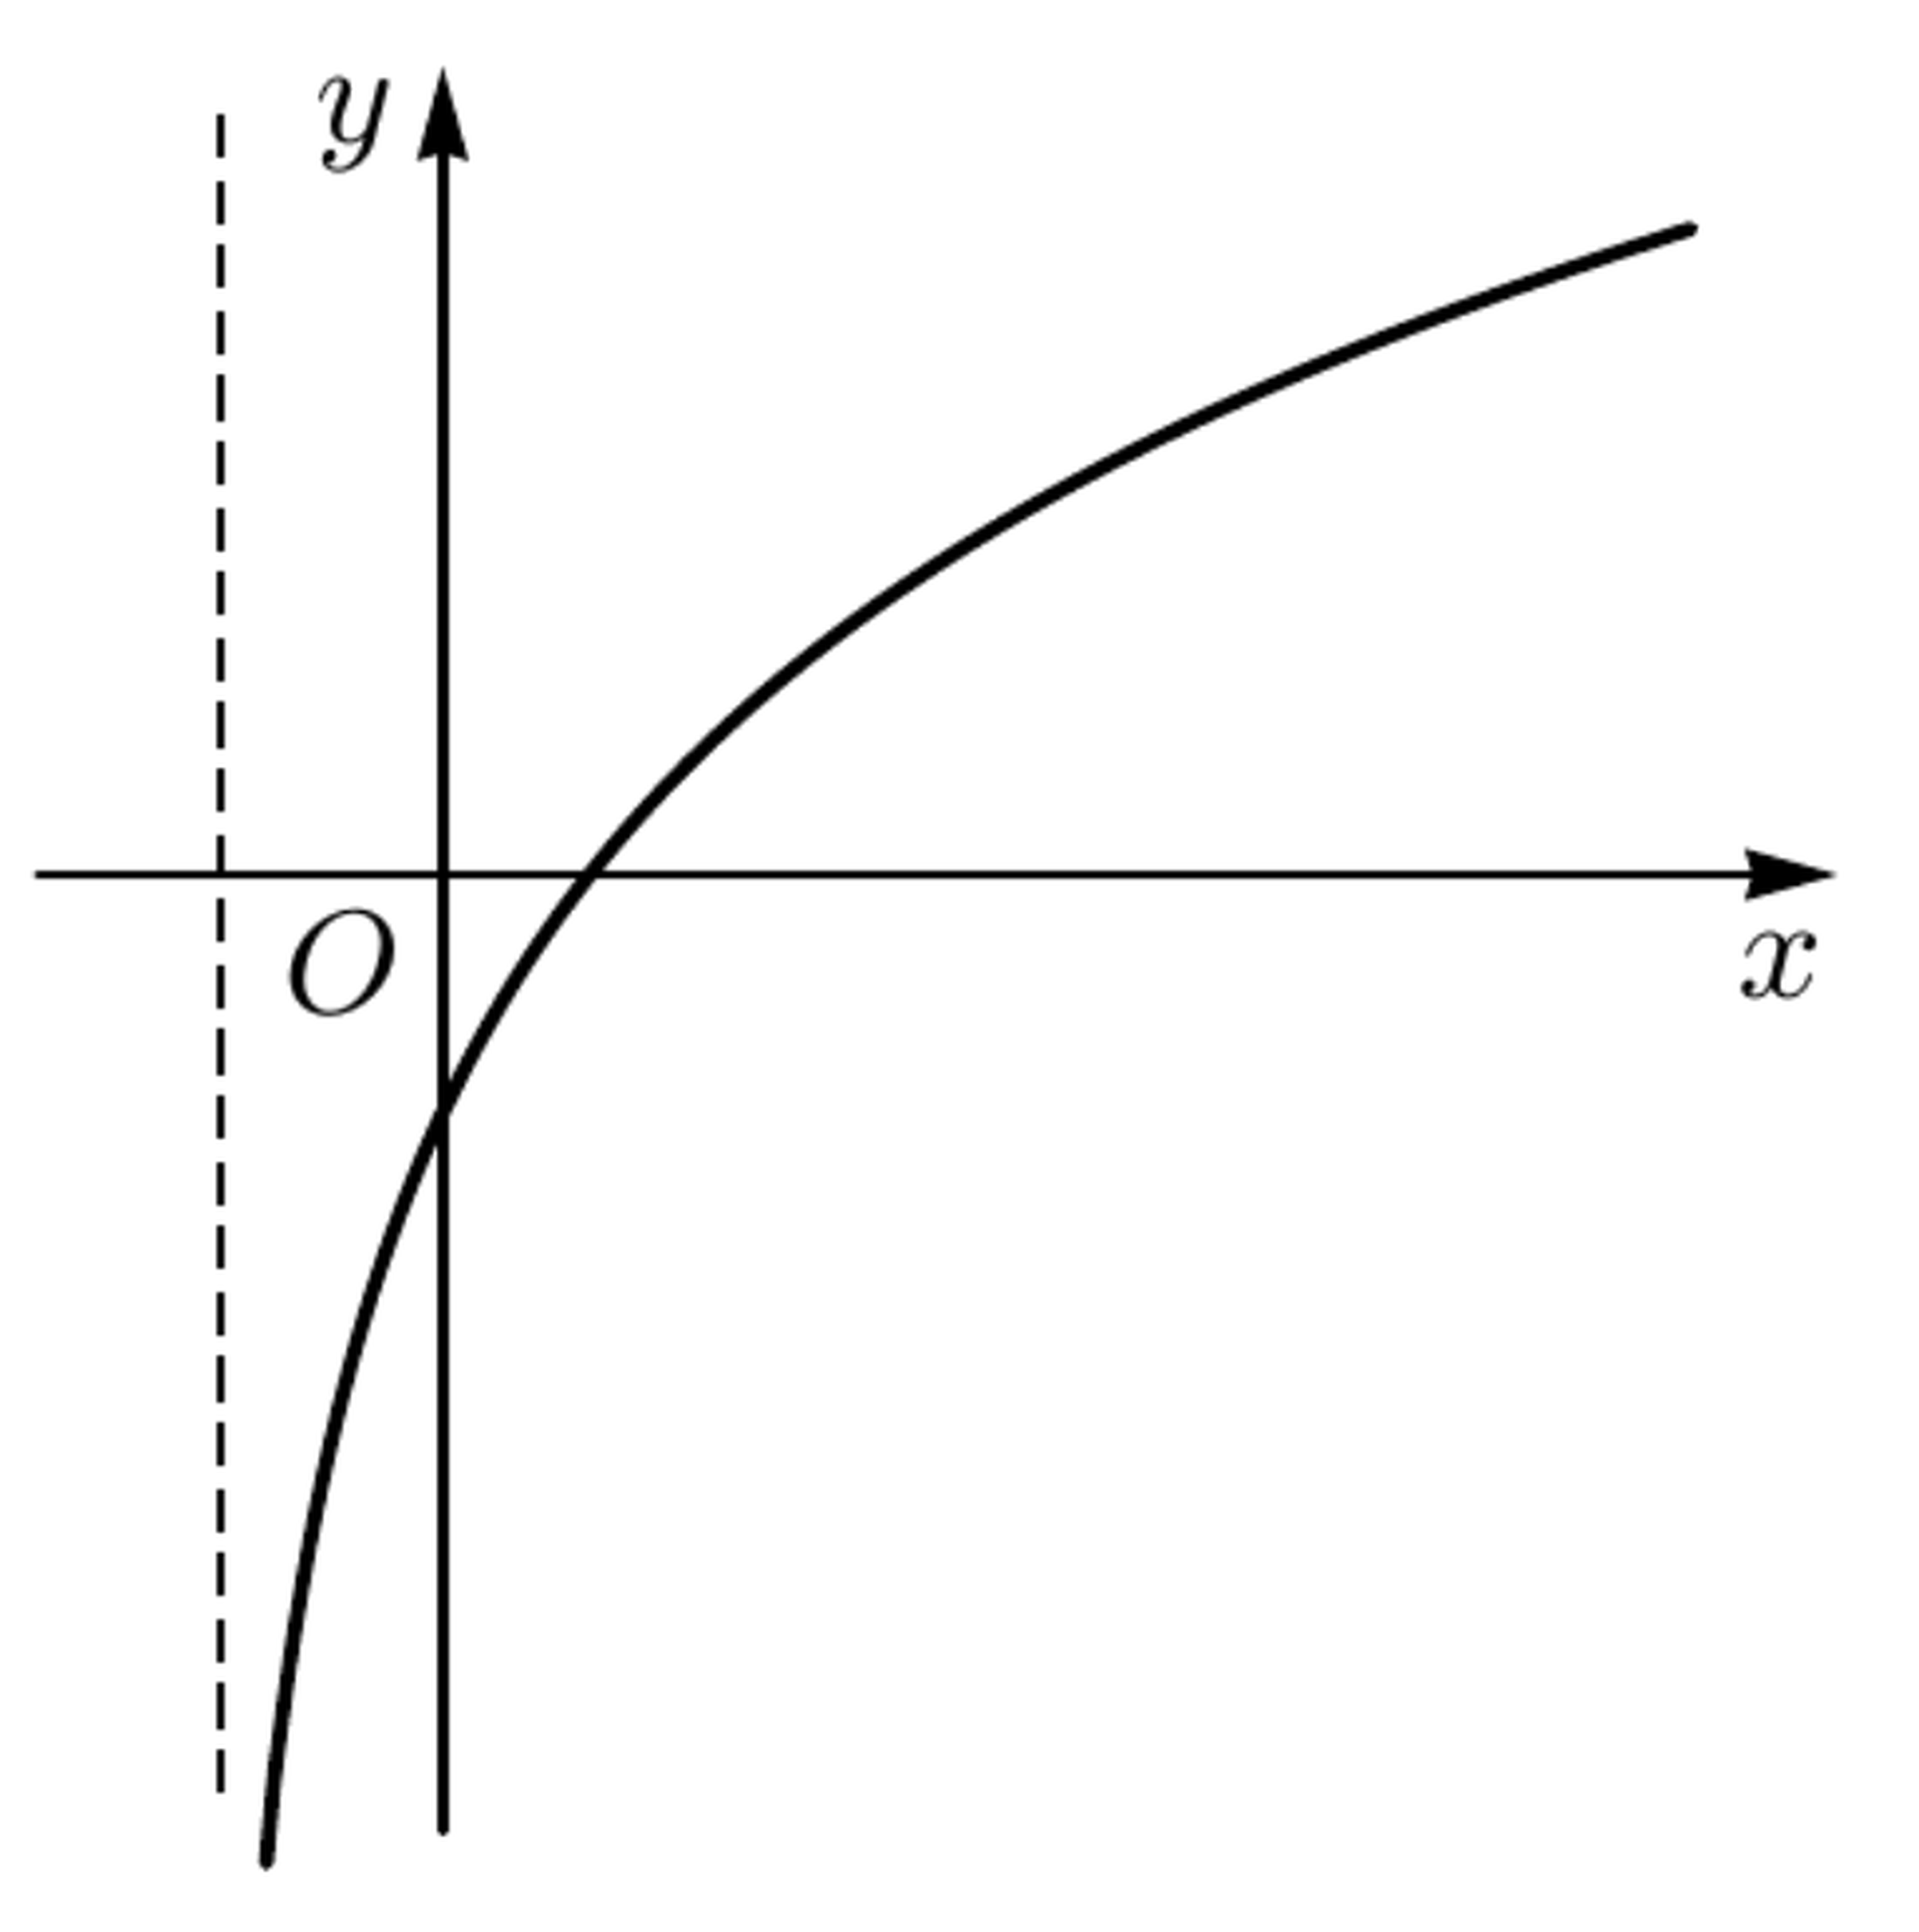
\includegraphics[width=0.42\textwidth]{figures/gao158_q15.png}
\end{center}

\keepwithprev
A. $a>1, b>1$\qquad\qquad B. $a>1, 0<b<1$

C. $0<a<1, b>1$\qquad\qquad D. $0<a<1, 0<b<1$

\ifanswer
\solbegin
\step{图像严格增，得 $a>1$.}
\step{图像与 $y$ 轴交于 $x$ 轴下方，得 $b>0$ 且 $\log_a b<0$，即 $0<b<1$，故选 $B$.}
\solend
\fi

% === Q16 === \lvert\log_2 x\rvert；解析 5 行，故选 C
\item 已知函数 $f(x)=\lvert\log_2 x\rvert$，若 $0<a<b$ 且 $f(a)=f(b)$，则 $a+2b$ 的取值范围是\mbox{（\quad）}

\keepwithprev
A. $(2\sqrt2,+\infty)$\qquad B. $[2\sqrt2,+\infty)$\qquad C. $(3,+\infty)$\qquad D. $[3,+\infty)$

\ifanswer
\solbegin
\step{由 $a<b$ 及 $\lvert\log_2 a\rvert=\lvert\log_2 b\rvert$，得 $\log_2 a=-\log_2 b$，即 $ab=1$，}
\step{且 $0<a<1<b$.}
\step{设 $t=a+2b=2b+\dfrac1b$，则 $t-3=\dfrac{(b-1)(2b-1)}{b}>0$.}
\step{反之，任取 $t>3$，令 $b=\dfrac{t+\sqrt{t^2-8}}{4}>1$、$a=\dfrac1b$，则满足题设且 $a+2b=t$.}
\step{因此取值范围为 $(3,+\infty)$，故选 $C$.}
\solend
\fi

\end{enumerate}

\bigsec{三、解答题}

\begin{enumerate}
\setcounter{enumi}{16}

% === Q17 === 集合、\overline{A}、\subseteq；解析 9 行
\item 已知全集 $U=\R$，集合 $A=\left\{x\mid\dfrac{x-3}{x+1}\leqslant0\right\}$，$B=\{x\mid x^2-2mx+m^2-9<0\}$（$m$ 为实数）.

(1) 当 $m=4$ 时，求 $A\cap B$ 和 $\overline{A}\cup B$；

(2) 若“$x\in A$”是“$x\in B$”的充分条件，求实数 $m$ 的取值范围.

\ifanswer
\solbegin
\step{(1) $\dfrac{x-3}{x+1}\leqslant0\Leftrightarrow-1<x\leqslant3$，所以 $A=(-1,3]$.}
\step{当 $m=4$ 时，$B=\{x\mid(x-4)^2<9\}=(1,7)$，}
\step{于是 $A\cap B=(1,3]$，$\overline{A}\cup B=(-\infty,-1]\cup(1,+\infty)$；}
\step{(2) $x^2-2mx+m^2-9<0\Leftrightarrow(x-m)^2<9$，所以 $B=(m-3,m+3)$.}
\step{题设充分条件等价于 $A\subseteq B$.}
\step{由于 $A=(-1,3]$，左端须满足 $m-3\leqslant-1$.}
\step{又 $3\in A$，须有 $3<m+3$.}
\step{这两个条件也保证 $(-1,3]\subseteq(m-3,m+3)$，}
\step{因此 $A\subseteq B\Leftrightarrow\begin{cases}m-3\leqslant-1\\m+3>3\end{cases}\Leftrightarrow0<m\leqslant2$.}
\solend
\fi

% === Q18 === 蓄水池造价（含 (3) 场地限制）；单位 \mathrm{m}；解析 13 行
\item 某工厂拟建一个容积为 $400\mathrm{m}^3$ 的无盖长方体蓄水池，池深 $4\mathrm{m}$，池底为矩形，其一边长
为 $x\mathrm{m}$. 池壁每平方米造价 100 元，池底每平方米造价 150 元. 设水池的总造价为 $C$
元.

(1) 把 $C$ 表示成 $x$ 的函数，并写出它的定义域；

(2) 当 $x$ 为何值时，总造价最低？最低造价是多少？

(3) 受场地限制，池底一边长 $x$ 不超过 $8\mathrm{m}$，此时总造价最低是多少？

\ifanswer
\solbegin
\step{(1) 设池底另一边长为 $y\mathrm{m}$，则 $4xy=400$，所以 $y=\dfrac{100}{x}$，$x>0$.}
\step{池底面积为 $100\mathrm{m}^2$，池壁总面积为 $8\left(x+\dfrac{100}{x}\right)\mathrm{m}^2$，}
\step{因此 $C(x)=100\times8\left(x+\dfrac{100}{x}\right)+150\times100=800x+\dfrac{80000}{x}+15000$，}
\step{定义域为 $(0,+\infty)$.}
\step{(2) 因为 $x>0$，所以 $C(x)=800\left(x+\dfrac{100}{x}\right)+15000$，}
\step{$\geqslant800\times2\sqrt{x\cdot\dfrac{100}{x}}+15000=31000$，}
\step{当且仅当 $x=\dfrac{100}{x}$，即 $x=10$ 时取等号.}
\step{答：当 $x=10$ 时，总造价最低，为 31000 元.}
\step{(3) 此时定义域为 $(0,8]$. 任取 $0<x_1<x_2\leqslant8$，}
\step{则 $C(x_2)-C(x_1)=800(x_2-x_1)\left(1-\dfrac{100}{x_1x_2}\right)<0$，}
\step{所以 $C(x)$ 在 $(0,8]$ 上严格递减，$x=8$ 时总造价最低，}
\step{且 $C(8)=800\times8+\dfrac{80000}{8}+15000=31400$.}
\step{答：受场地限制时，最低总造价为 31400 元.}
\solend
\fi

% === Q19 === 甲乙滤材 0.8^n／0.7^n；解析 17 行
\item 某环保公司研发了两种新型滤材甲和乙：污水每经过一层甲滤材，污染物含量减少
20\%；每经过一层乙滤材，污染物含量减少 30\%. 每层甲滤材成本 3 万元，每层乙滤材
成本 4 万元. 设原污水中污染物含量为 1，要求处理后污染物含量低于原来的 5\%.

(1) 若只使用一种滤材，污水经过 $n$ 层后污染物含量为 $y$，分别写出使用甲、乙两种滤材
时 $y$ 关于 $n$ 的函数关系式（$n$ 为正整数）；

(2) 若只使用一种滤材，分别求甲、乙至少各需要多少层，并比较哪种滤材的总成本更
低；

(3) 若两种滤材可以混合使用（先后顺序不影响效果），设使用甲滤材 $m$ 层、乙滤材 $n$
层（$m$、$n$ 为非负整数），求满足要求的最低总成本，并指出此时 $m$、$n$ 的值.

\ifanswer
\solbegin
\step{(1) 甲：$y=0.8^n$；乙：$y=0.7^n$，其中 $n$ 为正整数.}
\step{(2) 两种滤材均须满足 $y<0.05$，且污染物含量随层数增加而严格减少.}
\step{$0.8^{14}\approx0.04398<0.05<0.05498\approx0.8^{13}$，}
\step{$0.7^9=0.040353607<0.05<0.05764801=0.7^8$，}
\step{甲至少需要 14 层，成本为 $3\times14=42$ 万元；}
\step{乙至少需要 9 层，成本为 $4\times9=36$ 万元.}
\step{因此，只使用一种滤材时，使用乙滤材的总成本更低.}
\step{(3) 设总成本为 $C$ 万元，则 $C=3m+4n,0.8^m\cdot0.7^n<0.05,m,n\in\{0,1,2,\cdots\}$，}
\step{若 $m\geqslant3$，将其中 3 层甲替换为 2 层乙，}
\step{因为 $0.7^2=0.49<0.512=0.8^3,2\times4<3\times3$，}
\step{替换后污染物含量更低，成本减少 1 万元，因此最低成本方案必有 $m\leqslant2$.}
\step{当 $m=0$ 时，由第（2）小题得至少需要 9 层乙，最低成本为 36 万元.}
\step{当 $m=1$ 或 $m=2$ 时，$0.8\cdot0.7^7>0.8^2\cdot0.7^7=0.052706752>0.05$，}
\step{$0.8^2\cdot0.7^8<0.8\cdot0.7^8=0.046118408<0.05$，}
\step{因此两种情形均至少需要 8 层乙，}
\step{对应最低成本分别为 $3+4\times8=35$ 万元，$3\times2+4\times8=38$ 万元.}
\step{答：满足要求的最低总成本为 35 万元，此时使用甲滤材 1 层、乙滤材 8 层.}
\solend
\fi

% === Q20 === f(x)=\log_2(4^x+1)-x；\Delta；解析 17 行
\item 已知函数 $f(x)=\log_2(4^x+1)-x$.

(1) 证明 $f(x)=\log_2(2^x+2^{-x})$，并求 $f(x)$ 的最小值及取得最小值时 $x$ 的值；

(2) 解不等式 $f(x)>\log_2 5-1$；

(3) 证明：函数 $f(x)$ 在区间 $[0,+\infty)$ 上是严格增函数；并求使关于 $x$ 的方程 $f(x)=m$ 恰
有两个不同实数解的实数 $m$ 的取值范围.

\ifanswer
\solbegin
\step{(1) $f(x)=\log_2(4^x+1)-\log_2 2^x=\log_2\dfrac{4^x+1}{2^x}=\log_2(2^x+2^{-x})$，}
\step{因为 $2^x+2^{-x}\geqslant2\sqrt{2^x\cdot2^{-x}}=2$，所以 $f(x)\geqslant\log_2 2=1$，}
\step{等号当且仅当 $2^x=2^{-x}$，即 $x=0$ 时成立，故最小值为 1.}
\step{(2) 令 $t=2^x>0$，则 $f(x)>\log_2 5-1\Leftrightarrow t+\dfrac1t>\dfrac52\Leftrightarrow2t^2-5t+2>0$}
\step{$\Leftrightarrow(2t-1)(t-2)>0$，}
\step{结合 $t>0$，得 $0<t<\dfrac12$ 或 $t>2$，即 $x<-1$ 或 $x>1$，}
\step{解集为 $(-\infty,-1)\cup(1,+\infty)$.}
\step{(3) 任取 $0\leqslant x_1<x_2$，记 $a=2^{x_1}$，$b=2^{x_2}$，则 $1\leqslant a<b$，$ab>1$，}
\step{从而 $\left(b+\dfrac1b\right)-\left(a+\dfrac1a\right)=(b-a)\left(1-\dfrac{1}{ab}\right)>0$，}
\step{由对数函数的严格递增性，得 $f(x_1)<f(x_2)$，}
\step{所以 $f(x)$ 在 $[0,+\infty)$ 上是严格增函数.}
\step{当 $m<1$ 时，由（1）得方程无实数解；当 $m=1$ 时，只有实数解 $x=0$.}
\step{当 $m>1$ 时，令 $t=2^x>0$，则 $f(x)=m\Leftrightarrow t+\dfrac1t=2^m\Leftrightarrow t^2-2^m t+1=0$，}
\step{此时 $\Delta=2^{2m}-4>0$，两根之和为 $2^m>0$、之积为 $1>0$，}
\step{故有两个不同的正根.}
\step{每个正根 $t$ 唯一确定一个实数 $x=\log_2 t$，故原方程恰有两个不同实数解，}
\step{所求范围为 $m\in(1,+\infty)$.}
\solend
\fi

% === Q21 === f(x)=4^x-m\cdot2^{x+1}+3 值域与 h(m) 分段；解析 13 行
\item 已知函数 $f(x)=4^x-m\cdot2^{x+1}+3$（$m\in\R$），$x\in[0,2]$.

(1) 当 $m=1$ 时，求 $f(x)$ 的值域；

(2) 记 $f(x)$ 的最小值为 $h(m)$，求 $h(m)$ 的表达式；

(3) 若关于 $x$ 的方程 $f(x)=0$ 在区间 $[0,2]$ 上有解，求实数 $m$ 的取值范围.

\ifanswer
\solbegin
\step{令 $t=2^x$，则 $t\in[1,4]$，且 $f(x)=t^2-2mt+3=(t-m)^2+3-m^2$，}
\step{(1) 当 $m=1$ 时，$f(x)=(t-1)^2+2$.}
\step{由 $0\leqslant t-1\leqslant3$，得 $2\leqslant f(x)\leqslant11$，值域为 $[2,11]$.}
\step{(2) 二次函数 $y=(t-m)^2+3-m^2$ 的对称轴为直线 $t=m$.}
\step{当 $m\leqslant1$ 时，在 $t=1$ 处取最小值；}
\step{当 $1<m<4$ 时，在 $t=m$ 处取最小值；}
\step{当 $m\geqslant4$ 时，在 $t=4$ 处取最小值；}
\step{因此 $h(m)=\begin{cases}4-2m,&m\leqslant1\\3-m^2,&1<m<4\\19-8m,&m\geqslant4\end{cases}$；}
\step{(3) 方程 $f(x)=0$ 在 $[0,2]$ 上有解，}
\step{等价于存在 $t\in[1,4]$，使 $m=\dfrac{t^2+3}{2t}=\dfrac12\left(t+\dfrac3t\right)$，}
\step{由基本不等式，$m\geqslant\dfrac12\cdot2\sqrt{t\cdot\dfrac3t}=\sqrt3$，当且仅当 $t=\sqrt3$ 时取等号；}
\step{又 $\dfrac{19}{8}-m=\dfrac{(4-t)(4t-3)}{8t}\geqslant0$，当且仅当 $t=4$ 时取等号；}
\step{因此必有 $\sqrt3\leqslant m\leqslant\dfrac{19}{8}$.}
\solend
\fi

\end{enumerate}

\end{document}
"
% 紧凑版：xelatex "\def\iscompact{1}% 高一158_上实东滩_期中.tex
%   —— 高一上数学"2026-2027 年上实东滩高一上期中"（试卷版/答案版/紧凑版）
% 试卷版：xelatex 高一158_上实东滩_期中.tex
% 答案版：xelatex "\def\isanswer{1}% 高一158_上实东滩_期中.tex
%   —— 高一上数学"2026-2027 年上实东滩高一上期中"（试卷版/答案版/紧凑版）
% 试卷版：xelatex 高一158_上实东滩_期中.tex
% 答案版：xelatex "\def\isanswer{1}\input{高一158_上实东滩_期中.tex}"
% 紧凑版：xelatex "\def\iscompact{1}\input{高一158_上实东滩_期中.tex}"
%
% ① 原始材料：微信公众号"魔都数学加油站"文章，连载"27学年高一158"，原文标题
% "27学年高一158——2026-2027年上海市上实东滩高一上期中"（本卷本地编号 158 与
% 原卷连载号一致，无撞号）。
% 正文为 9 张 PNG 页（01/05/08/09 为 2560×3620，02/03/04/06/07 为 4762×6735，
% 同一篇各页分辨率混排，逐页按各自分辨率裁图核对）。
% 体例：讲评版——填空 3—12（10 题）、选择 13—16（4 题）、解答 17—21（5 题），
% 共 19 题，自第 3 题起编（1、2 未印在本篇）；Q5 只印【答案】、其余 18 题
% 逐题印【解析】（逐题核实，见 ②）。题目、答案、解析均据原图转录；卷面粉红色
% 水印"魔都数学加油站"及公众号页脚未录入。全卷末题为第 21 题，无附加题节。
% 全卷 2 组配图（逐页通读 9 页确认）——
%   · Q10 题干右侧"曼 → man"字形变换图（02 页），题目配图、三版都出，
%     裁 figures/gao158_q10.png；
%   · Q15 题干"如图所示"对数函数大致图像（03 页右下），题目配图、三版都出，
%     裁 figures/gao158_q15.png；
% 2 图均取自原卷截图，去粉色水印、转灰度、4× LANCZOS 放大；
% 其余各页逐页确认无其它题目配图、无解析内配图、无表格。
%
% 卷首标题：原卷印作"2026-2027 年上实东滩高一上期中"，年份区间按全稿惯例排 en dash；
% 原卷卷面未印副标题，本稿按同期中卷知识模块口径补出"集合与常用逻辑用语、不等式、函数"。
%
% ② 与原卷的排版差异／照录项清单：
%   ① 原文从第 3 题起，本稿保留原题号；共 19 题三节，解答题 5 题到 21；
%      三节各自一个 enumerate＋各自 \setcounter{enumi}{2}／{12}／{16}，
%      不贯穿（题目溯源.py 按 \bigsec 切节、每节独立计 depth，只收 depth==1 的 \item）；
%   ② 混合体例：Q5 只印【答案】、无【解析】，按 高一156 第 3 题成例另提
%      \ans{}、不补造解析；其余 18 题印【解析】、用 \solbegin…\solend；
%      四道选择题答案均在解析末句"故选 C／B／B／C"（逐个放大复核）、
%      题干括号 \mbox{（\quad）} 留空、不另提 \ans{}；答案版
%      【答案】/【解析】标记数 = 19 = 全卷题数（1 个 \ans ＋ 18 个 \solbegin）；
%   ③ 原卷卷面未印副标题，本稿按知识模块口径补出；
%   ④ 原卷填空横线按全稿惯例排 \blankline[4.4em]；选择题选项段前按惯例各加
%      \keepwithprev；解答题不留作答区、不加 \anspace（原卷为讲评版）；
%   ⑤ 数集：Q13"在 \R 上严格递增"、Q14"$x\in\R$"、Q17"$U=\R$"、
%      Q21"$m\in\R$" 原卷印正体粗体 R，按全稿惯例归一 \R；
%      绝对值排 \lvert…\rvert（Q12 $\lvert a\rvert$、Q14 $\lvert x-2\rvert$、
%      Q16 $\lvert\log_2 x\rvert$／$\lvert\log_2 a\rvert$／$\lvert\log_2 b\rvert$），
%      集合描述竖线排 \mid（Q17），不等号按全稿惯例排 \leqslant／\geqslant，
%      补集上划线 \overline{A}（Q17）；
%   ⑥ 子集／真子集符号逐处照录不统一：Q14 解析"$(2,3)\subsetneq(1,3)$"原卷印
%      带下划线且被斜杠划过的 ⊊（真子集，放大 03 页确认），照录 \subsetneq；
%      Q17 解析三处"$A\subseteq B$""$(-1,3]\subseteq(m-3,m+3)$"原卷印
%      带下划线 ⊆（放大 05 页确认），照录 \subseteq；本卷无单线 \subset 用例；
%   ⑦ 判别式：Q20 (3) 解析"$\Delta=2^{2m}-4>0$"原卷印高瘦等腰 \Delta
%      （像素实测高/宽 ≈ 1.13，扁三角 \triangle 为 0.93，放大 08 页确认），
%      照录 \Delta；本卷无扁三角 \triangle 用例；
%   ⑧ "图像"与"图象"：全卷统一用"图像"（Q6 题干、Q10 两处、Q11 解析、
%      Q15 题干与解析两处，逐处放大确认带单人旁），照录不改；
%   ⑨ 中文弯引号照录：Q5 命题"若实数…"、Q10"曼""man""新"、Q14 题干与
%      解析的两则不等式、Q17 (2)"$x\in A$""$x\in B$"；注释里一律 ASCII 引号；
%   ⑩ 半角逗号逐处照录：Q8"$2,3,4$""$-2,-1,0$"、Q10 点坐标 $(x,y)$／
%      $(t,2^t-1)$／$(1-2^t,t)$、Q15 四选项"$a>1, b>1$"等、
%      Q19 (3)"$C=3m+4n,0.8^m\cdot0.7^n<0.05,m,n\in\{0,1,2,\cdots\}$"
%      与"$0.7^2=0.49<0.512=0.8^3,2\times4<3\times3$"、
%      Q21 cases 内"$4-2m,$"等；其余行中逗号／顿号照录全角；
%      行末西文句点 ASCII `.`；
%   ⑪ 顿号照录：Q3"（用 $a$、$b$ 表示）"、Q5"$x$、$y$"、Q13"A、B"、
%      Q16 解析"$>1$、$a=\dfrac1b$"、Q19"甲、乙""$m$、$n$"、
%      Q20"$2^m>0$、之积为"、Q21"$m$、$n$"；顿号一律移到数学模式外，
%      数学模式内不出现中文标点；
%   ⑫ 角度与单位照录：Q10 三处"$90^{\circ}$"、Q18"$400\mathrm{m}^3$"
%      "$4\mathrm{m}$""$x\mathrm{m}$""$8\mathrm{m}$""$y\mathrm{m}$"
%      "$100\mathrm{m}^2$""$\left(x+\dfrac{100}{x}\right)\mathrm{m}^2$"；
%      Q19 百分号"20\%""30\%""5\%"按原卷排 \%；
%   ⑬ 文本模式全角括号照录：Q10"（提示：…）"、Q17"（$m$ 为实数）"、
%      Q19"（$n$ 为正整数）""（先后顺序不影响效果）""（$m$、$n$ 为非负整数）"、
%      Q20"由（1）得"、Q19"由第（2）小题"、Q21"（$m\in\R$）"；
%      子题行首标号按全稿惯例用半角 (1)(2)(3)；
%   ⑭ 复杂式照录别简化：Q3 $\dfrac{\log_3 2+\log_3 5}{\log_3 3+2\log_3 2}$、
%      Q8 $[-3,-2)\cup(4,5]$、Q9 $18ab=2^t\cdot3^t=6^t=a+b$、
%      Q12 $\dfrac{\sqrt6}{2}$、Q18 $C(8)=800\times8+\dfrac{80000}{8}+15000=31400$
%      （原卷即 C(8)，非 C(2)）、Q19 $0.8^{14}\approx0.04398$、
%      $0.7^9=0.040353607$、$0.052706752$、$0.046118408$、
%      Q20 $t^2-2^m t+1=0$、Q21 $h(m)$ 三段 cases 与 $\dfrac{(4-t)(4t-3)}{8t}$ 等；
%      \left…\right 不得拆到不同 $…$ 组；cases 块整体算一个印刷行；
%   ⑮ 一条 \step = 原卷解析的一个印刷行；别并折行、别拆行。跨页续印按题合并
%      （Q7 的 01—02 页、Q9/Q10/Q11 的 02—03 页、Q13/Q14 的 03 页上下、
%      Q15/Q16 的 04 页上下、Q17 的 04—05 页、Q18 的 05—06 页、
%      Q19 的 06—07 页、Q20 的 07—08 页、Q21 的 08—09 页）；
%      跨半页重叠行（Q5【答案】、Q9 设公共值行、Q10 题干、Q16 反之行、
%      Q18 (2) 题干、Q19 末两行、Q20 (3) 末行、Q21 cases 块）只算一个印刷行；
%   ⑯ 配图：2 组题目配图（见 ①），均三版都出，\needvspace 守卫放 \item 之前
%      把"题干＋图"整块推走，\includegraphics 放题干之后；本卷无解析内配图、
%      无红字加粗小标题（全卷逐页确认，故无 \stepm）。
%
% ③ 行数复核：一条 \step = 原卷解析的一个印刷行，cases 块作一个印刷行计。
%   逐题数（逐页核对）：Q3：1；Q4：2；Q5：0（只印【答案】、提 \ans{}，
%   不计入 \step 账）；Q6：1；Q7：4；Q8：5；Q9：2；Q10：2；Q11：3；
%   Q12：3；Q13：2；Q14：3；Q15：2；Q16：5；Q17：9；Q18：13；
%   Q19：17；Q20：17；Q21：13。
%   合计 104 行（104 条 \step ＋ 0 条 \stepm），与原卷逐题印刷行相等。
%   全卷 19 题：Q5 一处 \ans{} ＋ 其余 18 题设 \solbegin…\solend，
%   答案版【答案】/【解析】标记数 = 19 = 全卷题数。
%
% ④ 页码分布（供回原图复核）：
%   卷首标题＋"一、填空题"＋Q3 题干＋解析 1 行、Q4 题干＋解析 2 行、
%   Q5 题干＋【答案】在 01 页上半；Q5【答案】（重叠重印）＋Q6 题干＋解析 1 行、
%   Q7 题干＋解析前 3 行在 01 页下半；Q7 解析末行＋Q8 题干＋解析 5 行、
%   Q9 题干＋解析首行在 02 页上半；Q9 解析末行＋Q10 题干（含"曼→man"图）
%   ＋解析 2 行＋Q11 题干＋解析首行在 02 页下半；Q11 解析后 2 行＋Q12 题干
%   ＋解析 3 行＋"二、选择题"标题＋Q13 题干＋选项在 03 页上半；
%   Q13 选项（重叠重印）＋解析 2 行＋Q14 题干＋选项＋解析 3 行＋Q15 题干
%   ＋对数图像（右侧）在 03 页下半；Q15 选项＋解析 2 行＋Q16 题干＋选项
%   ＋解析前 4 行在 04 页上半；Q16 解析末行＋"三、解答题"标题＋Q17 题干
%   ＋两问＋解析 (1) 3 行在 04 页下半；Q17 解析 (2) 6 行＋Q18 题干＋三问
%   ＋解析 (1) 4 行＋(2) 首行在 05 页上下；Q18 解析 (2) 后 3 行＋(3) 5 行
%   ＋Q19 题干＋三问＋解析 (1) 1 行＋(2) 3 行在 06 页上下；Q19 解析 (2) 3 行
%   ＋(3) 12 行在 07 页上半；Q19 解析末 2 行（重叠）＋Q20 题干＋三问
%   ＋解析 (1) 3 行在 07 页下半；Q20 解析 (2) 4 行＋(3) 前 4 行在 08 页上半；
%   Q20 解析 (3) 后 6 行＋Q21 题干＋(1) 问在 08 页下半；Q21 (2)(3) 问＋
%   解析 (1) 3 行＋(2) 5 行＋cases 块在 09 页上半；Q21 cases 块（重叠）
%   ＋(3) 解析 5 行在 09 页下半。本稿按题连排，不丢行、不并折行；
%   全卷末题为第 21 题，无附加题节。
%
% ⑤ 存疑／需主会话回原图复核：
%   1. Q14 解析"$(2,3)\subsetneq(1,3)$"的 ⊊（真子集带斜杠）与 Q17 的 ⊆
%      是两种不同记号，本稿分别照录 \subsetneq／\subseteq，请复核；
%   2. Q20 (3)"$\Delta=2^{2m}-4>0$"判为高瘦 \Delta，请复核是否 \triangle；
%   3. 任务书提示"Q18 解析里印 C(2)=…"，但 06 页原图逐处读作
%      $C(8)=800\times8+\dfrac{80000}{8}+15000=31400$，未找到 C(2)，
%      本稿照原卷排 C(8)，请复核；
%   4. Q19 解析末句"最低总成本为 35 万元"（07 页上下两处印同），
%      OCR 曾误读为 34，本稿按 35 照录，请复核；
%   5. Q10 提示末尾"坐标为 $(-y,x)$）."为半角 $)$＋全角 $）$ 两枚括号，
%      本稿照录，请复核；
%   6. Q21 cases 块后"；"落在分式中行右侧（排版居中基线所致），
%      本稿排作 $…\end{cases}$；，请复核。
%   全卷除此 6 类外未发现其它笔误／自相矛盾处；19 题中 18 题印【解析】。
%
\documentclass[a4paper,11pt]{article}
\usepackage{common}

\begin{document}

\examtitlest[3]{2026--2027 年上实东滩高一上期中}{集合与常用逻辑用语、不等式、函数}

\bigsec{一、填空题}

\begin{enumerate}
\setcounter{enumi}{2}

% === Q3 === 换底公式；解析 1 行
\item 已知 $3^a=5$，$\log_3 2=b$，则 $\log_{12} 10=$\blankline[4.4em]（用 $a$、$b$ 表示）.

\ifanswer
\solbegin
\step{$\log_{12} 10=\dfrac{\log_3 2+\log_3 5}{\log_3 3+2\log_3 2}=\dfrac{a+b}{1+2b}$.}
\solend
\fi

% === Q4 === 定义域；解析 2 行；半角括号 ( ) 与全角逗号照录
\item 函数 $y=\sqrt{2-x}+\lg(x^2-1)$ 的定义域为\blankline[4.4em].

\ifanswer
\solbegin
\step{由 $2-x\geqslant0$ 且 $x^2-1>0$，得 $x\leqslant2$ 且 ($x<-1$或$x>1$)，}
\step{定义域为 $(-\infty,-1)\cup(1,2]$.}
\solend
\fi

% === Q5 === 只印【答案】、无【解析】；反证法，中文弯引号
\item 用反证法证明命题“若实数 $x$、$y$ 满足 $x+y>2$，则 $x$、$y$ 中至少有一个大于 1”时，
应假设\blankline[4.4em].

\ifanswer
\ans{$x\leqslant1$ 且 $y\leqslant1$}
\fi

% === Q6 === 图像平移；解析 1 行
\item 函数 $y=\dfrac{2x+1}{x-1}$ 的图像可由函数 $y=\dfrac{3}{x}$ 的图像先向右平移 $a$ 个单位，再向上平移 $b$ 个单位
得到，则 $a+b=$\blankline[4.4em].

\ifanswer
\solbegin
\step{$y=\dfrac{2x+1}{x-1}=\dfrac{3}{x-1}+2$，所以 $a=1$，$b=2$，$a+b=3$.}
\solend
\fi

% === Q7 === 集合三元子集；解析 4 行，跨 01—02 页
\item 设 $A=\{a_1,a_2,a_3,a_4\}$ 是由四个实数组成的集合，若 $A$ 的所有三元子集中，三个元素之和
组成的集合为 $B=\{1,4,7,12\}$，则集合 $A=$\blankline[4.4em].

\ifanswer
\solbegin
\step{设 $S=a_1+a_2+a_3+a_4$，}
\step{每个元素在四个三元子集中恰出现三次，则 $3S=1+4+7+12=24$，得 $S=8$.}
\step{四个三元子集的元素和分别为 $S-a_i$，}
\step{所以 $A=\{8-1,8-4,8-7,8-12\}=\{-4,1,4,7\}$.}
\solend
\fi

% === Q8 === 不等式整数解；解析 5 行；半角逗号照录
\item 不等式 $x^2-(a+1)x+a<0$ 的解集中恰有 3 个整数，则 $a$ 的取值范围是\blankline[4.4em].

\ifanswer
\solbegin
\step{原不等式为 $(x-1)(x-a)<0$；}
\step{$a=1$ 时解集为空集，不符合题意.}
\step{若 $a>1$，解集为 $(1,a)$，恰含整数 $2,3,4$，则 $4<a\leqslant5$.}
\step{若 $a<1$，解集为 $(a,1)$，恰含整数 $-2,-1,0$，则 $-3\leqslant a<-2$.}
\step{故 $a$ 的取值范围是 $[-3,-2)\cup(4,5]$.}
\solend
\fi

% === Q9 === 对数换底＋指数；解析 2 行
\item 已知正数 $a$、$b$ 满足 $1+\log_2 a=2+\log_3 b=\log_6(a+b)$，则 $\dfrac1a+\dfrac1b=$\blankline[4.4em].

\ifanswer
\solbegin
\step{设公共值为 $t$，则 $2a=2^t$，$9b=3^t$，$a+b=6^t$，}
\step{于是 $18ab=2^t\cdot3^t=6^t=a+b$，即 $\dfrac1a+\dfrac1b=\dfrac{a+b}{ab}=18$.}
\solend
\fi

% === Q10 === "曼"字旋转 90°；题目配图（三版都出）；解析 2 行
\needvspace{6cm}
\item 网上流传一个有趣的字形变换：把汉字“曼”的右半部分旋转 $90^{\circ}$，就得到英文单词
“man”的艺术字. 数学中，把曲线绕原点旋转也会得到“新”的曲线：将函数
$y=2^x-1$ 的图像绕坐标原点 $O$ 逆时针旋转 $90^{\circ}$，得到的曲线恰是某个函数的
图像，则这个函数的解析式为\blankline[4.4em]（提示：点 $(x,y)$ 绕 $O$ 逆时针旋转 $90^{\circ}$ 后的
坐标为 $(-y,x)$）.

\begin{center}

\includegraphics[width=0.42\textwidth]{figures/gao158_q10.png}
\end{center}

\ifanswer
\solbegin
\step{原图像上的点 $(t,2^t-1)$ 旋转后为 $(1-2^t,t)$.}
\step{记其为 $(x,y)$，则 $x=1-2^y$，即 $y=\log_2(1-x)$，定义域为 $(-\infty,1)$.}
\solend
\fi

% === Q11 === 值域；解析 3 行，跨 02—03 页
\item 函数 $f(x)=\sqrt{x-2}-\sqrt{15-3x}$ 的值域为\blankline[4.4em].

\ifanswer
\solbegin
\step{由 $x-2\geqslant0$ 且 $15-3x\geqslant0$，得定义域为 $[2,5]$.}
\step{在 $[2,5]$ 上，$\sqrt{x-2}$ 与 $-\sqrt{15-3x}$ 均严格递增，因此 $f(x)$ 严格递增.}
\step{$f(2)=-3$，$f(5)=\sqrt3$，结合函数的图像，值域为 $[-3,\sqrt3]$.}
\solend
\fi

% === Q12 === 绝对值 \lvert…\rvert；解析 3 行
\item 设实数 $a$ 满足 $a<4a^3-5a<\lvert a\rvert$，则 $a$ 的取值范围是\blankline[4.4em].

\ifanswer
\solbegin
\step{由 $a<\lvert a\rvert$ 得 $a<0$，原不等式为 $a<4a^3-5a<-a$.}
\step{同除以 $a<0$，得 $1>4a^2-5>-1\Leftrightarrow1<a^2<\dfrac32$，结合 $a<0$，}
\step{得 $-\dfrac{\sqrt6}{2}<a<-1$，故解集为 $\left(-\dfrac{\sqrt6}{2},-1\right)$.}
\solend
\fi

\end{enumerate}

\bigsec{二、选择题}

\begin{enumerate}
\setcounter{enumi}{12}

% === Q13 === \R 归一；解析 2 行，故选 C
\item 已知 $a>b$，则下列不等式一定成立的是\mbox{（\quad）}

\keepwithprev
A. $\dfrac1a<\dfrac1b$\qquad B. $a^2>b^2$\qquad C. $a^3>b^3$\qquad D. $ac^2>bc^2$

\ifanswer
\solbegin
\step{幂函数 $y=x^3$ 在 $\R$ 上严格递增，$a>b\Rightarrow a^3>b^3$，C 正确.}
\step{取 $a=1$，$b=-1$ 得 A、B 不成立；取 $c=0$ 得 D 不成立；故选 $C$.}
\solend
\fi

% === Q14 === \subsetneq 真子集；解析 3 行，故选 B
\item 设 $x\in\R$，则“$\lvert x-2\rvert<1$”是“$x^2-5x+6<0$”的\mbox{（\quad）}

\keepwithprev
A. 充分非必要条件\qquad\qquad B. 必要非充分条件

C. 充要条件\qquad\qquad D. 既非充分又非必要条件

\ifanswer
\solbegin
\step{$\lvert x-2\rvert<1\Leftrightarrow1<x<3$，$x^2-5x+6<0\Leftrightarrow(x-2)(x-3)<0\Leftrightarrow2<x<3$.}
\step{由 $(2,3)\subsetneq(1,3)$，得“$\lvert x-2\rvert<1$”是“$x^2-5x+6<0$”的必要非充分条件，}
\step{故选 $B$.}
\solend
\fi

% === Q15 === 对数函数大致图像（题目配图，三版都出）；解析 2 行，故选 B
\needvspace{9cm}
\item 已知函数 $f(x)=\log_a(x+b)$（$a>0$ 且 $a\ne1$）的大致图像如图所示，则 $a$、$b$ 满足
的关系是\mbox{（\quad）}

\begin{center}
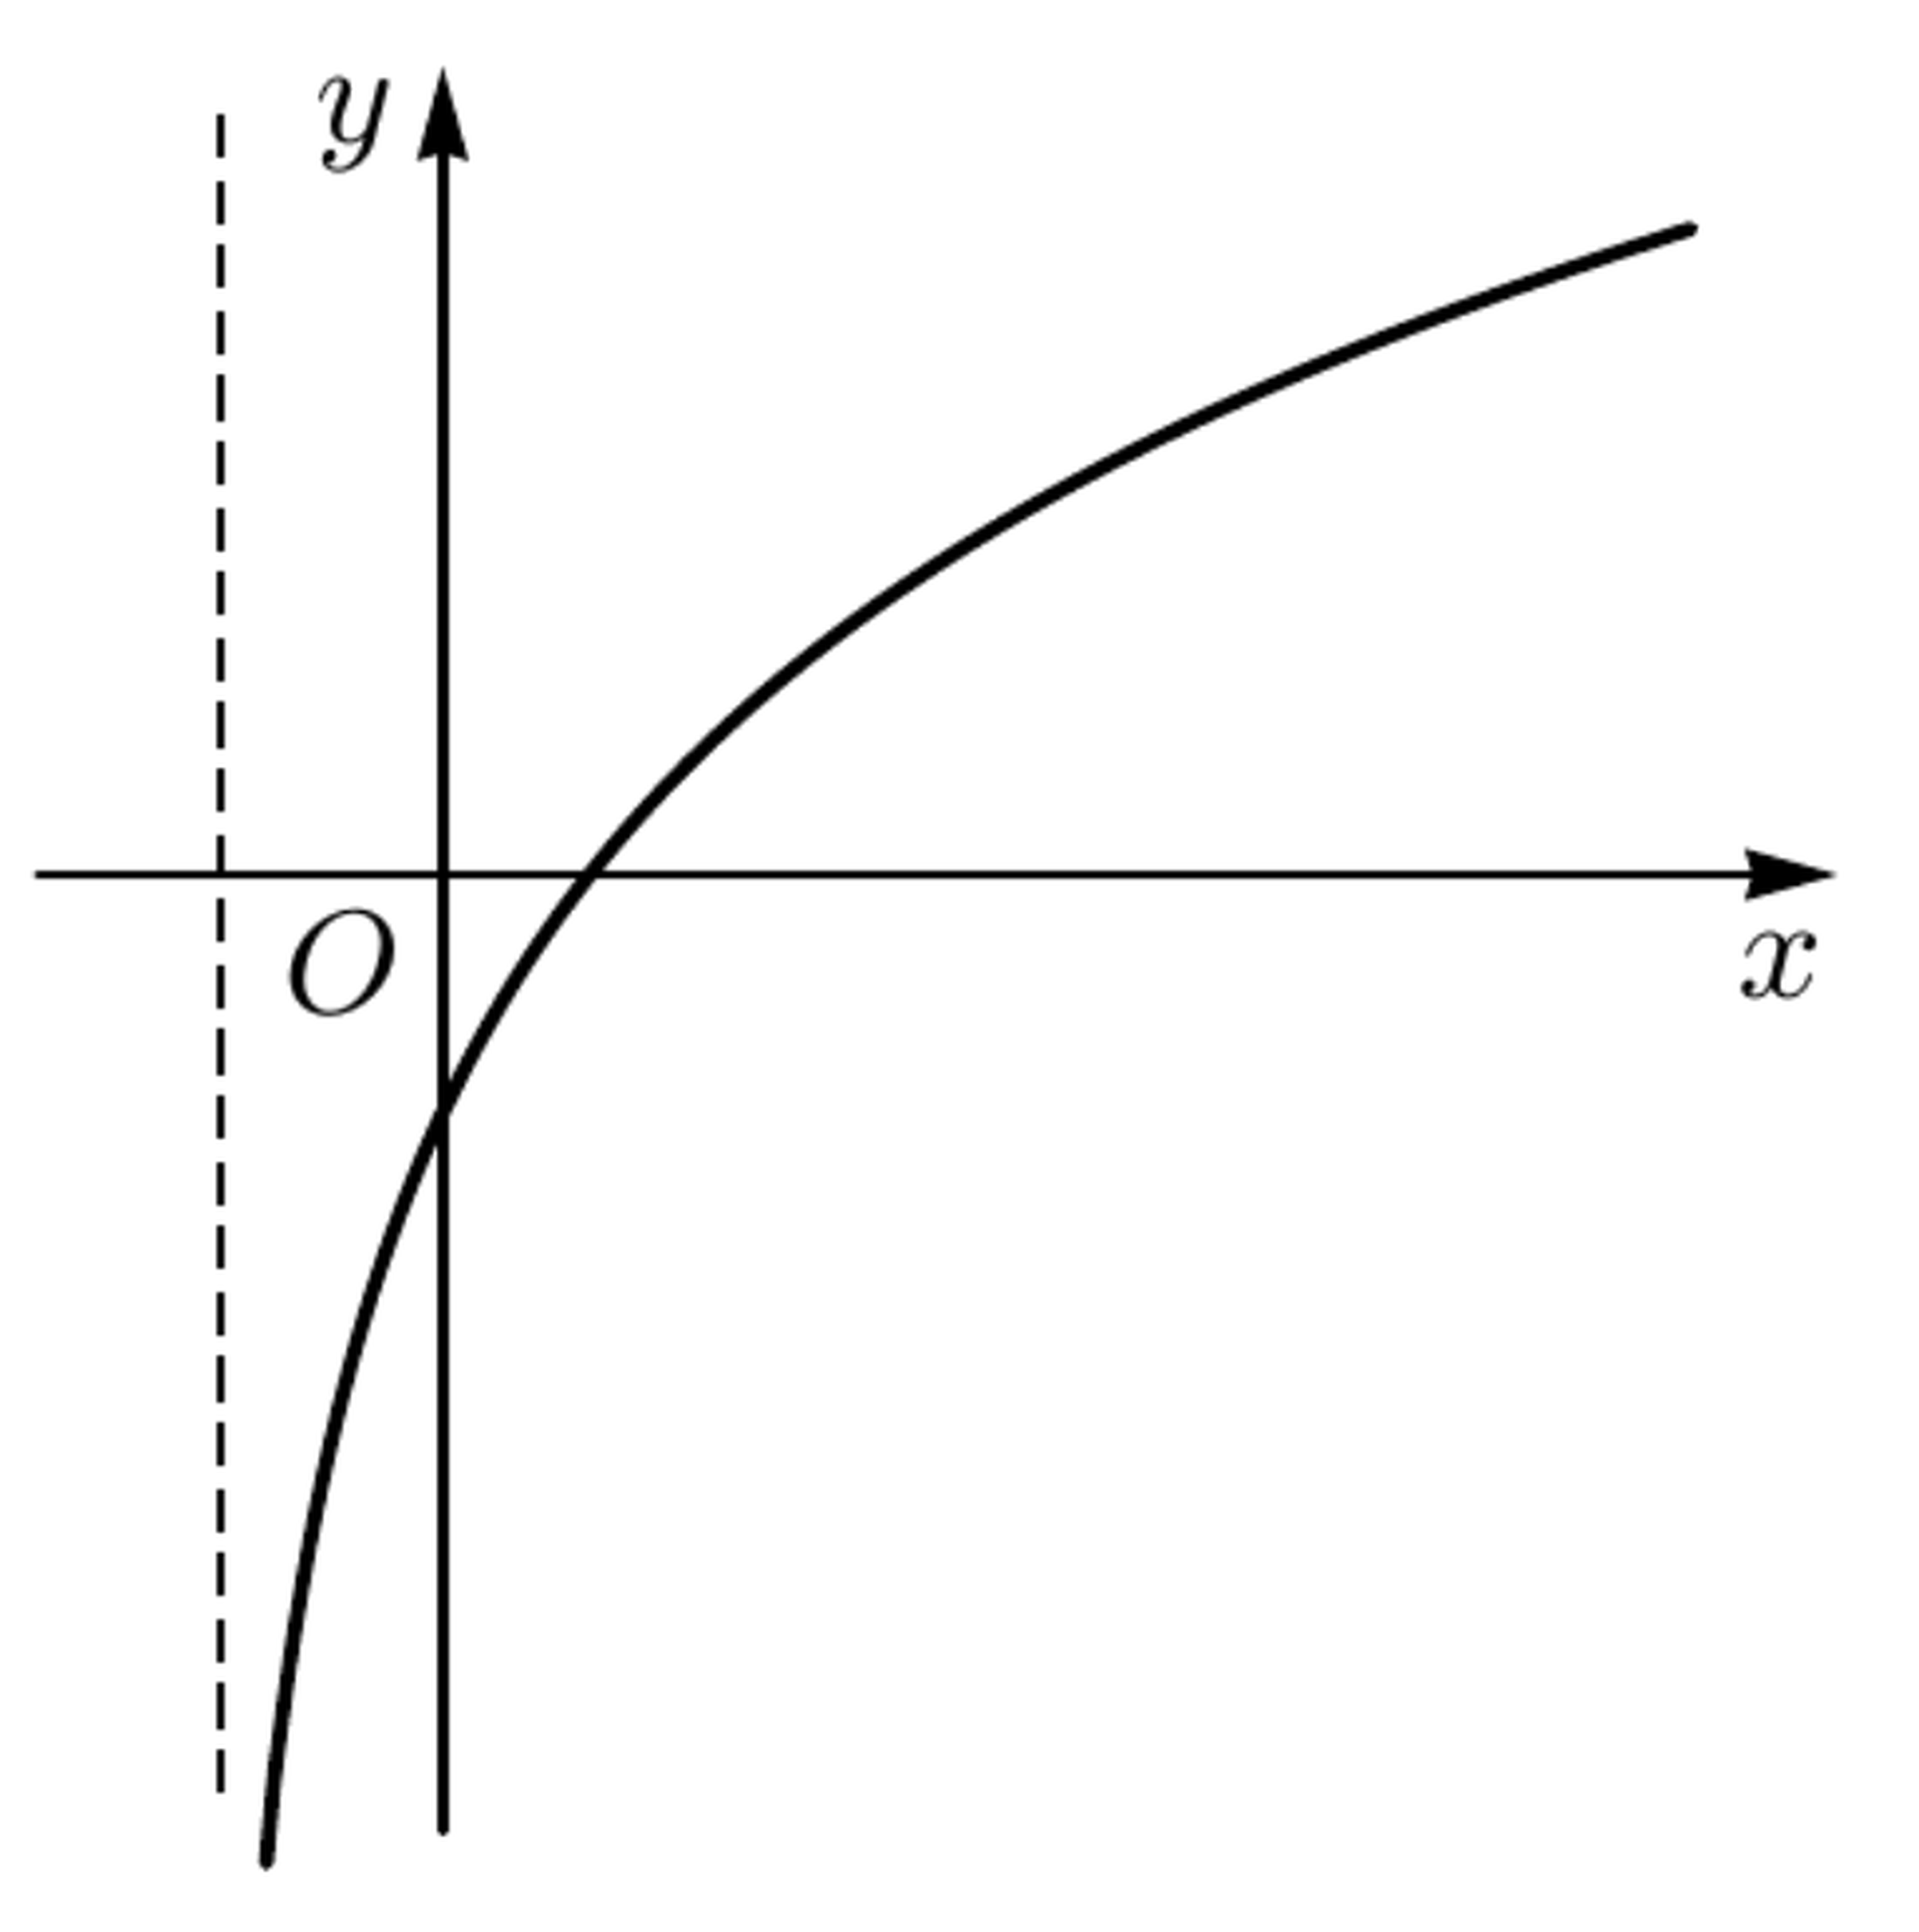
\includegraphics[width=0.42\textwidth]{figures/gao158_q15.png}
\end{center}

\keepwithprev
A. $a>1, b>1$\qquad\qquad B. $a>1, 0<b<1$

C. $0<a<1, b>1$\qquad\qquad D. $0<a<1, 0<b<1$

\ifanswer
\solbegin
\step{图像严格增，得 $a>1$.}
\step{图像与 $y$ 轴交于 $x$ 轴下方，得 $b>0$ 且 $\log_a b<0$，即 $0<b<1$，故选 $B$.}
\solend
\fi

% === Q16 === \lvert\log_2 x\rvert；解析 5 行，故选 C
\item 已知函数 $f(x)=\lvert\log_2 x\rvert$，若 $0<a<b$ 且 $f(a)=f(b)$，则 $a+2b$ 的取值范围是\mbox{（\quad）}

\keepwithprev
A. $(2\sqrt2,+\infty)$\qquad B. $[2\sqrt2,+\infty)$\qquad C. $(3,+\infty)$\qquad D. $[3,+\infty)$

\ifanswer
\solbegin
\step{由 $a<b$ 及 $\lvert\log_2 a\rvert=\lvert\log_2 b\rvert$，得 $\log_2 a=-\log_2 b$，即 $ab=1$，}
\step{且 $0<a<1<b$.}
\step{设 $t=a+2b=2b+\dfrac1b$，则 $t-3=\dfrac{(b-1)(2b-1)}{b}>0$.}
\step{反之，任取 $t>3$，令 $b=\dfrac{t+\sqrt{t^2-8}}{4}>1$、$a=\dfrac1b$，则满足题设且 $a+2b=t$.}
\step{因此取值范围为 $(3,+\infty)$，故选 $C$.}
\solend
\fi

\end{enumerate}

\bigsec{三、解答题}

\begin{enumerate}
\setcounter{enumi}{16}

% === Q17 === 集合、\overline{A}、\subseteq；解析 9 行
\item 已知全集 $U=\R$，集合 $A=\left\{x\mid\dfrac{x-3}{x+1}\leqslant0\right\}$，$B=\{x\mid x^2-2mx+m^2-9<0\}$（$m$ 为实数）.

(1) 当 $m=4$ 时，求 $A\cap B$ 和 $\overline{A}\cup B$；

(2) 若“$x\in A$”是“$x\in B$”的充分条件，求实数 $m$ 的取值范围.

\ifanswer
\solbegin
\step{(1) $\dfrac{x-3}{x+1}\leqslant0\Leftrightarrow-1<x\leqslant3$，所以 $A=(-1,3]$.}
\step{当 $m=4$ 时，$B=\{x\mid(x-4)^2<9\}=(1,7)$，}
\step{于是 $A\cap B=(1,3]$，$\overline{A}\cup B=(-\infty,-1]\cup(1,+\infty)$；}
\step{(2) $x^2-2mx+m^2-9<0\Leftrightarrow(x-m)^2<9$，所以 $B=(m-3,m+3)$.}
\step{题设充分条件等价于 $A\subseteq B$.}
\step{由于 $A=(-1,3]$，左端须满足 $m-3\leqslant-1$.}
\step{又 $3\in A$，须有 $3<m+3$.}
\step{这两个条件也保证 $(-1,3]\subseteq(m-3,m+3)$，}
\step{因此 $A\subseteq B\Leftrightarrow\begin{cases}m-3\leqslant-1\\m+3>3\end{cases}\Leftrightarrow0<m\leqslant2$.}
\solend
\fi

% === Q18 === 蓄水池造价（含 (3) 场地限制）；单位 \mathrm{m}；解析 13 行
\item 某工厂拟建一个容积为 $400\mathrm{m}^3$ 的无盖长方体蓄水池，池深 $4\mathrm{m}$，池底为矩形，其一边长
为 $x\mathrm{m}$. 池壁每平方米造价 100 元，池底每平方米造价 150 元. 设水池的总造价为 $C$
元.

(1) 把 $C$ 表示成 $x$ 的函数，并写出它的定义域；

(2) 当 $x$ 为何值时，总造价最低？最低造价是多少？

(3) 受场地限制，池底一边长 $x$ 不超过 $8\mathrm{m}$，此时总造价最低是多少？

\ifanswer
\solbegin
\step{(1) 设池底另一边长为 $y\mathrm{m}$，则 $4xy=400$，所以 $y=\dfrac{100}{x}$，$x>0$.}
\step{池底面积为 $100\mathrm{m}^2$，池壁总面积为 $8\left(x+\dfrac{100}{x}\right)\mathrm{m}^2$，}
\step{因此 $C(x)=100\times8\left(x+\dfrac{100}{x}\right)+150\times100=800x+\dfrac{80000}{x}+15000$，}
\step{定义域为 $(0,+\infty)$.}
\step{(2) 因为 $x>0$，所以 $C(x)=800\left(x+\dfrac{100}{x}\right)+15000$，}
\step{$\geqslant800\times2\sqrt{x\cdot\dfrac{100}{x}}+15000=31000$，}
\step{当且仅当 $x=\dfrac{100}{x}$，即 $x=10$ 时取等号.}
\step{答：当 $x=10$ 时，总造价最低，为 31000 元.}
\step{(3) 此时定义域为 $(0,8]$. 任取 $0<x_1<x_2\leqslant8$，}
\step{则 $C(x_2)-C(x_1)=800(x_2-x_1)\left(1-\dfrac{100}{x_1x_2}\right)<0$，}
\step{所以 $C(x)$ 在 $(0,8]$ 上严格递减，$x=8$ 时总造价最低，}
\step{且 $C(8)=800\times8+\dfrac{80000}{8}+15000=31400$.}
\step{答：受场地限制时，最低总造价为 31400 元.}
\solend
\fi

% === Q19 === 甲乙滤材 0.8^n／0.7^n；解析 17 行
\item 某环保公司研发了两种新型滤材甲和乙：污水每经过一层甲滤材，污染物含量减少
20\%；每经过一层乙滤材，污染物含量减少 30\%. 每层甲滤材成本 3 万元，每层乙滤材
成本 4 万元. 设原污水中污染物含量为 1，要求处理后污染物含量低于原来的 5\%.

(1) 若只使用一种滤材，污水经过 $n$ 层后污染物含量为 $y$，分别写出使用甲、乙两种滤材
时 $y$ 关于 $n$ 的函数关系式（$n$ 为正整数）；

(2) 若只使用一种滤材，分别求甲、乙至少各需要多少层，并比较哪种滤材的总成本更
低；

(3) 若两种滤材可以混合使用（先后顺序不影响效果），设使用甲滤材 $m$ 层、乙滤材 $n$
层（$m$、$n$ 为非负整数），求满足要求的最低总成本，并指出此时 $m$、$n$ 的值.

\ifanswer
\solbegin
\step{(1) 甲：$y=0.8^n$；乙：$y=0.7^n$，其中 $n$ 为正整数.}
\step{(2) 两种滤材均须满足 $y<0.05$，且污染物含量随层数增加而严格减少.}
\step{$0.8^{14}\approx0.04398<0.05<0.05498\approx0.8^{13}$，}
\step{$0.7^9=0.040353607<0.05<0.05764801=0.7^8$，}
\step{甲至少需要 14 层，成本为 $3\times14=42$ 万元；}
\step{乙至少需要 9 层，成本为 $4\times9=36$ 万元.}
\step{因此，只使用一种滤材时，使用乙滤材的总成本更低.}
\step{(3) 设总成本为 $C$ 万元，则 $C=3m+4n,0.8^m\cdot0.7^n<0.05,m,n\in\{0,1,2,\cdots\}$，}
\step{若 $m\geqslant3$，将其中 3 层甲替换为 2 层乙，}
\step{因为 $0.7^2=0.49<0.512=0.8^3,2\times4<3\times3$，}
\step{替换后污染物含量更低，成本减少 1 万元，因此最低成本方案必有 $m\leqslant2$.}
\step{当 $m=0$ 时，由第（2）小题得至少需要 9 层乙，最低成本为 36 万元.}
\step{当 $m=1$ 或 $m=2$ 时，$0.8\cdot0.7^7>0.8^2\cdot0.7^7=0.052706752>0.05$，}
\step{$0.8^2\cdot0.7^8<0.8\cdot0.7^8=0.046118408<0.05$，}
\step{因此两种情形均至少需要 8 层乙，}
\step{对应最低成本分别为 $3+4\times8=35$ 万元，$3\times2+4\times8=38$ 万元.}
\step{答：满足要求的最低总成本为 35 万元，此时使用甲滤材 1 层、乙滤材 8 层.}
\solend
\fi

% === Q20 === f(x)=\log_2(4^x+1)-x；\Delta；解析 17 行
\item 已知函数 $f(x)=\log_2(4^x+1)-x$.

(1) 证明 $f(x)=\log_2(2^x+2^{-x})$，并求 $f(x)$ 的最小值及取得最小值时 $x$ 的值；

(2) 解不等式 $f(x)>\log_2 5-1$；

(3) 证明：函数 $f(x)$ 在区间 $[0,+\infty)$ 上是严格增函数；并求使关于 $x$ 的方程 $f(x)=m$ 恰
有两个不同实数解的实数 $m$ 的取值范围.

\ifanswer
\solbegin
\step{(1) $f(x)=\log_2(4^x+1)-\log_2 2^x=\log_2\dfrac{4^x+1}{2^x}=\log_2(2^x+2^{-x})$，}
\step{因为 $2^x+2^{-x}\geqslant2\sqrt{2^x\cdot2^{-x}}=2$，所以 $f(x)\geqslant\log_2 2=1$，}
\step{等号当且仅当 $2^x=2^{-x}$，即 $x=0$ 时成立，故最小值为 1.}
\step{(2) 令 $t=2^x>0$，则 $f(x)>\log_2 5-1\Leftrightarrow t+\dfrac1t>\dfrac52\Leftrightarrow2t^2-5t+2>0$}
\step{$\Leftrightarrow(2t-1)(t-2)>0$，}
\step{结合 $t>0$，得 $0<t<\dfrac12$ 或 $t>2$，即 $x<-1$ 或 $x>1$，}
\step{解集为 $(-\infty,-1)\cup(1,+\infty)$.}
\step{(3) 任取 $0\leqslant x_1<x_2$，记 $a=2^{x_1}$，$b=2^{x_2}$，则 $1\leqslant a<b$，$ab>1$，}
\step{从而 $\left(b+\dfrac1b\right)-\left(a+\dfrac1a\right)=(b-a)\left(1-\dfrac{1}{ab}\right)>0$，}
\step{由对数函数的严格递增性，得 $f(x_1)<f(x_2)$，}
\step{所以 $f(x)$ 在 $[0,+\infty)$ 上是严格增函数.}
\step{当 $m<1$ 时，由（1）得方程无实数解；当 $m=1$ 时，只有实数解 $x=0$.}
\step{当 $m>1$ 时，令 $t=2^x>0$，则 $f(x)=m\Leftrightarrow t+\dfrac1t=2^m\Leftrightarrow t^2-2^m t+1=0$，}
\step{此时 $\Delta=2^{2m}-4>0$，两根之和为 $2^m>0$、之积为 $1>0$，}
\step{故有两个不同的正根.}
\step{每个正根 $t$ 唯一确定一个实数 $x=\log_2 t$，故原方程恰有两个不同实数解，}
\step{所求范围为 $m\in(1,+\infty)$.}
\solend
\fi

% === Q21 === f(x)=4^x-m\cdot2^{x+1}+3 值域与 h(m) 分段；解析 13 行
\item 已知函数 $f(x)=4^x-m\cdot2^{x+1}+3$（$m\in\R$），$x\in[0,2]$.

(1) 当 $m=1$ 时，求 $f(x)$ 的值域；

(2) 记 $f(x)$ 的最小值为 $h(m)$，求 $h(m)$ 的表达式；

(3) 若关于 $x$ 的方程 $f(x)=0$ 在区间 $[0,2]$ 上有解，求实数 $m$ 的取值范围.

\ifanswer
\solbegin
\step{令 $t=2^x$，则 $t\in[1,4]$，且 $f(x)=t^2-2mt+3=(t-m)^2+3-m^2$，}
\step{(1) 当 $m=1$ 时，$f(x)=(t-1)^2+2$.}
\step{由 $0\leqslant t-1\leqslant3$，得 $2\leqslant f(x)\leqslant11$，值域为 $[2,11]$.}
\step{(2) 二次函数 $y=(t-m)^2+3-m^2$ 的对称轴为直线 $t=m$.}
\step{当 $m\leqslant1$ 时，在 $t=1$ 处取最小值；}
\step{当 $1<m<4$ 时，在 $t=m$ 处取最小值；}
\step{当 $m\geqslant4$ 时，在 $t=4$ 处取最小值；}
\step{因此 $h(m)=\begin{cases}4-2m,&m\leqslant1\\3-m^2,&1<m<4\\19-8m,&m\geqslant4\end{cases}$；}
\step{(3) 方程 $f(x)=0$ 在 $[0,2]$ 上有解，}
\step{等价于存在 $t\in[1,4]$，使 $m=\dfrac{t^2+3}{2t}=\dfrac12\left(t+\dfrac3t\right)$，}
\step{由基本不等式，$m\geqslant\dfrac12\cdot2\sqrt{t\cdot\dfrac3t}=\sqrt3$，当且仅当 $t=\sqrt3$ 时取等号；}
\step{又 $\dfrac{19}{8}-m=\dfrac{(4-t)(4t-3)}{8t}\geqslant0$，当且仅当 $t=4$ 时取等号；}
\step{因此必有 $\sqrt3\leqslant m\leqslant\dfrac{19}{8}$.}
\solend
\fi

\end{enumerate}

\end{document}
"
% 紧凑版：xelatex "\def\iscompact{1}% 高一158_上实东滩_期中.tex
%   —— 高一上数学"2026-2027 年上实东滩高一上期中"（试卷版/答案版/紧凑版）
% 试卷版：xelatex 高一158_上实东滩_期中.tex
% 答案版：xelatex "\def\isanswer{1}\input{高一158_上实东滩_期中.tex}"
% 紧凑版：xelatex "\def\iscompact{1}\input{高一158_上实东滩_期中.tex}"
%
% ① 原始材料：微信公众号"魔都数学加油站"文章，连载"27学年高一158"，原文标题
% "27学年高一158——2026-2027年上海市上实东滩高一上期中"（本卷本地编号 158 与
% 原卷连载号一致，无撞号）。
% 正文为 9 张 PNG 页（01/05/08/09 为 2560×3620，02/03/04/06/07 为 4762×6735，
% 同一篇各页分辨率混排，逐页按各自分辨率裁图核对）。
% 体例：讲评版——填空 3—12（10 题）、选择 13—16（4 题）、解答 17—21（5 题），
% 共 19 题，自第 3 题起编（1、2 未印在本篇）；Q5 只印【答案】、其余 18 题
% 逐题印【解析】（逐题核实，见 ②）。题目、答案、解析均据原图转录；卷面粉红色
% 水印"魔都数学加油站"及公众号页脚未录入。全卷末题为第 21 题，无附加题节。
% 全卷 2 组配图（逐页通读 9 页确认）——
%   · Q10 题干右侧"曼 → man"字形变换图（02 页），题目配图、三版都出，
%     裁 figures/gao158_q10.png；
%   · Q15 题干"如图所示"对数函数大致图像（03 页右下），题目配图、三版都出，
%     裁 figures/gao158_q15.png；
% 2 图均取自原卷截图，去粉色水印、转灰度、4× LANCZOS 放大；
% 其余各页逐页确认无其它题目配图、无解析内配图、无表格。
%
% 卷首标题：原卷印作"2026-2027 年上实东滩高一上期中"，年份区间按全稿惯例排 en dash；
% 原卷卷面未印副标题，本稿按同期中卷知识模块口径补出"集合与常用逻辑用语、不等式、函数"。
%
% ② 与原卷的排版差异／照录项清单：
%   ① 原文从第 3 题起，本稿保留原题号；共 19 题三节，解答题 5 题到 21；
%      三节各自一个 enumerate＋各自 \setcounter{enumi}{2}／{12}／{16}，
%      不贯穿（题目溯源.py 按 \bigsec 切节、每节独立计 depth，只收 depth==1 的 \item）；
%   ② 混合体例：Q5 只印【答案】、无【解析】，按 高一156 第 3 题成例另提
%      \ans{}、不补造解析；其余 18 题印【解析】、用 \solbegin…\solend；
%      四道选择题答案均在解析末句"故选 C／B／B／C"（逐个放大复核）、
%      题干括号 \mbox{（\quad）} 留空、不另提 \ans{}；答案版
%      【答案】/【解析】标记数 = 19 = 全卷题数（1 个 \ans ＋ 18 个 \solbegin）；
%   ③ 原卷卷面未印副标题，本稿按知识模块口径补出；
%   ④ 原卷填空横线按全稿惯例排 \blankline[4.4em]；选择题选项段前按惯例各加
%      \keepwithprev；解答题不留作答区、不加 \anspace（原卷为讲评版）；
%   ⑤ 数集：Q13"在 \R 上严格递增"、Q14"$x\in\R$"、Q17"$U=\R$"、
%      Q21"$m\in\R$" 原卷印正体粗体 R，按全稿惯例归一 \R；
%      绝对值排 \lvert…\rvert（Q12 $\lvert a\rvert$、Q14 $\lvert x-2\rvert$、
%      Q16 $\lvert\log_2 x\rvert$／$\lvert\log_2 a\rvert$／$\lvert\log_2 b\rvert$），
%      集合描述竖线排 \mid（Q17），不等号按全稿惯例排 \leqslant／\geqslant，
%      补集上划线 \overline{A}（Q17）；
%   ⑥ 子集／真子集符号逐处照录不统一：Q14 解析"$(2,3)\subsetneq(1,3)$"原卷印
%      带下划线且被斜杠划过的 ⊊（真子集，放大 03 页确认），照录 \subsetneq；
%      Q17 解析三处"$A\subseteq B$""$(-1,3]\subseteq(m-3,m+3)$"原卷印
%      带下划线 ⊆（放大 05 页确认），照录 \subseteq；本卷无单线 \subset 用例；
%   ⑦ 判别式：Q20 (3) 解析"$\Delta=2^{2m}-4>0$"原卷印高瘦等腰 \Delta
%      （像素实测高/宽 ≈ 1.13，扁三角 \triangle 为 0.93，放大 08 页确认），
%      照录 \Delta；本卷无扁三角 \triangle 用例；
%   ⑧ "图像"与"图象"：全卷统一用"图像"（Q6 题干、Q10 两处、Q11 解析、
%      Q15 题干与解析两处，逐处放大确认带单人旁），照录不改；
%   ⑨ 中文弯引号照录：Q5 命题"若实数…"、Q10"曼""man""新"、Q14 题干与
%      解析的两则不等式、Q17 (2)"$x\in A$""$x\in B$"；注释里一律 ASCII 引号；
%   ⑩ 半角逗号逐处照录：Q8"$2,3,4$""$-2,-1,0$"、Q10 点坐标 $(x,y)$／
%      $(t,2^t-1)$／$(1-2^t,t)$、Q15 四选项"$a>1, b>1$"等、
%      Q19 (3)"$C=3m+4n,0.8^m\cdot0.7^n<0.05,m,n\in\{0,1,2,\cdots\}$"
%      与"$0.7^2=0.49<0.512=0.8^3,2\times4<3\times3$"、
%      Q21 cases 内"$4-2m,$"等；其余行中逗号／顿号照录全角；
%      行末西文句点 ASCII `.`；
%   ⑪ 顿号照录：Q3"（用 $a$、$b$ 表示）"、Q5"$x$、$y$"、Q13"A、B"、
%      Q16 解析"$>1$、$a=\dfrac1b$"、Q19"甲、乙""$m$、$n$"、
%      Q20"$2^m>0$、之积为"、Q21"$m$、$n$"；顿号一律移到数学模式外，
%      数学模式内不出现中文标点；
%   ⑫ 角度与单位照录：Q10 三处"$90^{\circ}$"、Q18"$400\mathrm{m}^3$"
%      "$4\mathrm{m}$""$x\mathrm{m}$""$8\mathrm{m}$""$y\mathrm{m}$"
%      "$100\mathrm{m}^2$""$\left(x+\dfrac{100}{x}\right)\mathrm{m}^2$"；
%      Q19 百分号"20\%""30\%""5\%"按原卷排 \%；
%   ⑬ 文本模式全角括号照录：Q10"（提示：…）"、Q17"（$m$ 为实数）"、
%      Q19"（$n$ 为正整数）""（先后顺序不影响效果）""（$m$、$n$ 为非负整数）"、
%      Q20"由（1）得"、Q19"由第（2）小题"、Q21"（$m\in\R$）"；
%      子题行首标号按全稿惯例用半角 (1)(2)(3)；
%   ⑭ 复杂式照录别简化：Q3 $\dfrac{\log_3 2+\log_3 5}{\log_3 3+2\log_3 2}$、
%      Q8 $[-3,-2)\cup(4,5]$、Q9 $18ab=2^t\cdot3^t=6^t=a+b$、
%      Q12 $\dfrac{\sqrt6}{2}$、Q18 $C(8)=800\times8+\dfrac{80000}{8}+15000=31400$
%      （原卷即 C(8)，非 C(2)）、Q19 $0.8^{14}\approx0.04398$、
%      $0.7^9=0.040353607$、$0.052706752$、$0.046118408$、
%      Q20 $t^2-2^m t+1=0$、Q21 $h(m)$ 三段 cases 与 $\dfrac{(4-t)(4t-3)}{8t}$ 等；
%      \left…\right 不得拆到不同 $…$ 组；cases 块整体算一个印刷行；
%   ⑮ 一条 \step = 原卷解析的一个印刷行；别并折行、别拆行。跨页续印按题合并
%      （Q7 的 01—02 页、Q9/Q10/Q11 的 02—03 页、Q13/Q14 的 03 页上下、
%      Q15/Q16 的 04 页上下、Q17 的 04—05 页、Q18 的 05—06 页、
%      Q19 的 06—07 页、Q20 的 07—08 页、Q21 的 08—09 页）；
%      跨半页重叠行（Q5【答案】、Q9 设公共值行、Q10 题干、Q16 反之行、
%      Q18 (2) 题干、Q19 末两行、Q20 (3) 末行、Q21 cases 块）只算一个印刷行；
%   ⑯ 配图：2 组题目配图（见 ①），均三版都出，\needvspace 守卫放 \item 之前
%      把"题干＋图"整块推走，\includegraphics 放题干之后；本卷无解析内配图、
%      无红字加粗小标题（全卷逐页确认，故无 \stepm）。
%
% ③ 行数复核：一条 \step = 原卷解析的一个印刷行，cases 块作一个印刷行计。
%   逐题数（逐页核对）：Q3：1；Q4：2；Q5：0（只印【答案】、提 \ans{}，
%   不计入 \step 账）；Q6：1；Q7：4；Q8：5；Q9：2；Q10：2；Q11：3；
%   Q12：3；Q13：2；Q14：3；Q15：2；Q16：5；Q17：9；Q18：13；
%   Q19：17；Q20：17；Q21：13。
%   合计 104 行（104 条 \step ＋ 0 条 \stepm），与原卷逐题印刷行相等。
%   全卷 19 题：Q5 一处 \ans{} ＋ 其余 18 题设 \solbegin…\solend，
%   答案版【答案】/【解析】标记数 = 19 = 全卷题数。
%
% ④ 页码分布（供回原图复核）：
%   卷首标题＋"一、填空题"＋Q3 题干＋解析 1 行、Q4 题干＋解析 2 行、
%   Q5 题干＋【答案】在 01 页上半；Q5【答案】（重叠重印）＋Q6 题干＋解析 1 行、
%   Q7 题干＋解析前 3 行在 01 页下半；Q7 解析末行＋Q8 题干＋解析 5 行、
%   Q9 题干＋解析首行在 02 页上半；Q9 解析末行＋Q10 题干（含"曼→man"图）
%   ＋解析 2 行＋Q11 题干＋解析首行在 02 页下半；Q11 解析后 2 行＋Q12 题干
%   ＋解析 3 行＋"二、选择题"标题＋Q13 题干＋选项在 03 页上半；
%   Q13 选项（重叠重印）＋解析 2 行＋Q14 题干＋选项＋解析 3 行＋Q15 题干
%   ＋对数图像（右侧）在 03 页下半；Q15 选项＋解析 2 行＋Q16 题干＋选项
%   ＋解析前 4 行在 04 页上半；Q16 解析末行＋"三、解答题"标题＋Q17 题干
%   ＋两问＋解析 (1) 3 行在 04 页下半；Q17 解析 (2) 6 行＋Q18 题干＋三问
%   ＋解析 (1) 4 行＋(2) 首行在 05 页上下；Q18 解析 (2) 后 3 行＋(3) 5 行
%   ＋Q19 题干＋三问＋解析 (1) 1 行＋(2) 3 行在 06 页上下；Q19 解析 (2) 3 行
%   ＋(3) 12 行在 07 页上半；Q19 解析末 2 行（重叠）＋Q20 题干＋三问
%   ＋解析 (1) 3 行在 07 页下半；Q20 解析 (2) 4 行＋(3) 前 4 行在 08 页上半；
%   Q20 解析 (3) 后 6 行＋Q21 题干＋(1) 问在 08 页下半；Q21 (2)(3) 问＋
%   解析 (1) 3 行＋(2) 5 行＋cases 块在 09 页上半；Q21 cases 块（重叠）
%   ＋(3) 解析 5 行在 09 页下半。本稿按题连排，不丢行、不并折行；
%   全卷末题为第 21 题，无附加题节。
%
% ⑤ 存疑／需主会话回原图复核：
%   1. Q14 解析"$(2,3)\subsetneq(1,3)$"的 ⊊（真子集带斜杠）与 Q17 的 ⊆
%      是两种不同记号，本稿分别照录 \subsetneq／\subseteq，请复核；
%   2. Q20 (3)"$\Delta=2^{2m}-4>0$"判为高瘦 \Delta，请复核是否 \triangle；
%   3. 任务书提示"Q18 解析里印 C(2)=…"，但 06 页原图逐处读作
%      $C(8)=800\times8+\dfrac{80000}{8}+15000=31400$，未找到 C(2)，
%      本稿照原卷排 C(8)，请复核；
%   4. Q19 解析末句"最低总成本为 35 万元"（07 页上下两处印同），
%      OCR 曾误读为 34，本稿按 35 照录，请复核；
%   5. Q10 提示末尾"坐标为 $(-y,x)$）."为半角 $)$＋全角 $）$ 两枚括号，
%      本稿照录，请复核；
%   6. Q21 cases 块后"；"落在分式中行右侧（排版居中基线所致），
%      本稿排作 $…\end{cases}$；，请复核。
%   全卷除此 6 类外未发现其它笔误／自相矛盾处；19 题中 18 题印【解析】。
%
\documentclass[a4paper,11pt]{article}
\usepackage{common}

\begin{document}

\examtitlest[3]{2026--2027 年上实东滩高一上期中}{集合与常用逻辑用语、不等式、函数}

\bigsec{一、填空题}

\begin{enumerate}
\setcounter{enumi}{2}

% === Q3 === 换底公式；解析 1 行
\item 已知 $3^a=5$，$\log_3 2=b$，则 $\log_{12} 10=$\blankline[4.4em]（用 $a$、$b$ 表示）.

\ifanswer
\solbegin
\step{$\log_{12} 10=\dfrac{\log_3 2+\log_3 5}{\log_3 3+2\log_3 2}=\dfrac{a+b}{1+2b}$.}
\solend
\fi

% === Q4 === 定义域；解析 2 行；半角括号 ( ) 与全角逗号照录
\item 函数 $y=\sqrt{2-x}+\lg(x^2-1)$ 的定义域为\blankline[4.4em].

\ifanswer
\solbegin
\step{由 $2-x\geqslant0$ 且 $x^2-1>0$，得 $x\leqslant2$ 且 ($x<-1$或$x>1$)，}
\step{定义域为 $(-\infty,-1)\cup(1,2]$.}
\solend
\fi

% === Q5 === 只印【答案】、无【解析】；反证法，中文弯引号
\item 用反证法证明命题“若实数 $x$、$y$ 满足 $x+y>2$，则 $x$、$y$ 中至少有一个大于 1”时，
应假设\blankline[4.4em].

\ifanswer
\ans{$x\leqslant1$ 且 $y\leqslant1$}
\fi

% === Q6 === 图像平移；解析 1 行
\item 函数 $y=\dfrac{2x+1}{x-1}$ 的图像可由函数 $y=\dfrac{3}{x}$ 的图像先向右平移 $a$ 个单位，再向上平移 $b$ 个单位
得到，则 $a+b=$\blankline[4.4em].

\ifanswer
\solbegin
\step{$y=\dfrac{2x+1}{x-1}=\dfrac{3}{x-1}+2$，所以 $a=1$，$b=2$，$a+b=3$.}
\solend
\fi

% === Q7 === 集合三元子集；解析 4 行，跨 01—02 页
\item 设 $A=\{a_1,a_2,a_3,a_4\}$ 是由四个实数组成的集合，若 $A$ 的所有三元子集中，三个元素之和
组成的集合为 $B=\{1,4,7,12\}$，则集合 $A=$\blankline[4.4em].

\ifanswer
\solbegin
\step{设 $S=a_1+a_2+a_3+a_4$，}
\step{每个元素在四个三元子集中恰出现三次，则 $3S=1+4+7+12=24$，得 $S=8$.}
\step{四个三元子集的元素和分别为 $S-a_i$，}
\step{所以 $A=\{8-1,8-4,8-7,8-12\}=\{-4,1,4,7\}$.}
\solend
\fi

% === Q8 === 不等式整数解；解析 5 行；半角逗号照录
\item 不等式 $x^2-(a+1)x+a<0$ 的解集中恰有 3 个整数，则 $a$ 的取值范围是\blankline[4.4em].

\ifanswer
\solbegin
\step{原不等式为 $(x-1)(x-a)<0$；}
\step{$a=1$ 时解集为空集，不符合题意.}
\step{若 $a>1$，解集为 $(1,a)$，恰含整数 $2,3,4$，则 $4<a\leqslant5$.}
\step{若 $a<1$，解集为 $(a,1)$，恰含整数 $-2,-1,0$，则 $-3\leqslant a<-2$.}
\step{故 $a$ 的取值范围是 $[-3,-2)\cup(4,5]$.}
\solend
\fi

% === Q9 === 对数换底＋指数；解析 2 行
\item 已知正数 $a$、$b$ 满足 $1+\log_2 a=2+\log_3 b=\log_6(a+b)$，则 $\dfrac1a+\dfrac1b=$\blankline[4.4em].

\ifanswer
\solbegin
\step{设公共值为 $t$，则 $2a=2^t$，$9b=3^t$，$a+b=6^t$，}
\step{于是 $18ab=2^t\cdot3^t=6^t=a+b$，即 $\dfrac1a+\dfrac1b=\dfrac{a+b}{ab}=18$.}
\solend
\fi

% === Q10 === "曼"字旋转 90°；题目配图（三版都出）；解析 2 行
\needvspace{6cm}
\item 网上流传一个有趣的字形变换：把汉字“曼”的右半部分旋转 $90^{\circ}$，就得到英文单词
“man”的艺术字. 数学中，把曲线绕原点旋转也会得到“新”的曲线：将函数
$y=2^x-1$ 的图像绕坐标原点 $O$ 逆时针旋转 $90^{\circ}$，得到的曲线恰是某个函数的
图像，则这个函数的解析式为\blankline[4.4em]（提示：点 $(x,y)$ 绕 $O$ 逆时针旋转 $90^{\circ}$ 后的
坐标为 $(-y,x)$）.

\begin{center}

\includegraphics[width=0.42\textwidth]{figures/gao158_q10.png}
\end{center}

\ifanswer
\solbegin
\step{原图像上的点 $(t,2^t-1)$ 旋转后为 $(1-2^t,t)$.}
\step{记其为 $(x,y)$，则 $x=1-2^y$，即 $y=\log_2(1-x)$，定义域为 $(-\infty,1)$.}
\solend
\fi

% === Q11 === 值域；解析 3 行，跨 02—03 页
\item 函数 $f(x)=\sqrt{x-2}-\sqrt{15-3x}$ 的值域为\blankline[4.4em].

\ifanswer
\solbegin
\step{由 $x-2\geqslant0$ 且 $15-3x\geqslant0$，得定义域为 $[2,5]$.}
\step{在 $[2,5]$ 上，$\sqrt{x-2}$ 与 $-\sqrt{15-3x}$ 均严格递增，因此 $f(x)$ 严格递增.}
\step{$f(2)=-3$，$f(5)=\sqrt3$，结合函数的图像，值域为 $[-3,\sqrt3]$.}
\solend
\fi

% === Q12 === 绝对值 \lvert…\rvert；解析 3 行
\item 设实数 $a$ 满足 $a<4a^3-5a<\lvert a\rvert$，则 $a$ 的取值范围是\blankline[4.4em].

\ifanswer
\solbegin
\step{由 $a<\lvert a\rvert$ 得 $a<0$，原不等式为 $a<4a^3-5a<-a$.}
\step{同除以 $a<0$，得 $1>4a^2-5>-1\Leftrightarrow1<a^2<\dfrac32$，结合 $a<0$，}
\step{得 $-\dfrac{\sqrt6}{2}<a<-1$，故解集为 $\left(-\dfrac{\sqrt6}{2},-1\right)$.}
\solend
\fi

\end{enumerate}

\bigsec{二、选择题}

\begin{enumerate}
\setcounter{enumi}{12}

% === Q13 === \R 归一；解析 2 行，故选 C
\item 已知 $a>b$，则下列不等式一定成立的是\mbox{（\quad）}

\keepwithprev
A. $\dfrac1a<\dfrac1b$\qquad B. $a^2>b^2$\qquad C. $a^3>b^3$\qquad D. $ac^2>bc^2$

\ifanswer
\solbegin
\step{幂函数 $y=x^3$ 在 $\R$ 上严格递增，$a>b\Rightarrow a^3>b^3$，C 正确.}
\step{取 $a=1$，$b=-1$ 得 A、B 不成立；取 $c=0$ 得 D 不成立；故选 $C$.}
\solend
\fi

% === Q14 === \subsetneq 真子集；解析 3 行，故选 B
\item 设 $x\in\R$，则“$\lvert x-2\rvert<1$”是“$x^2-5x+6<0$”的\mbox{（\quad）}

\keepwithprev
A. 充分非必要条件\qquad\qquad B. 必要非充分条件

C. 充要条件\qquad\qquad D. 既非充分又非必要条件

\ifanswer
\solbegin
\step{$\lvert x-2\rvert<1\Leftrightarrow1<x<3$，$x^2-5x+6<0\Leftrightarrow(x-2)(x-3)<0\Leftrightarrow2<x<3$.}
\step{由 $(2,3)\subsetneq(1,3)$，得“$\lvert x-2\rvert<1$”是“$x^2-5x+6<0$”的必要非充分条件，}
\step{故选 $B$.}
\solend
\fi

% === Q15 === 对数函数大致图像（题目配图，三版都出）；解析 2 行，故选 B
\needvspace{9cm}
\item 已知函数 $f(x)=\log_a(x+b)$（$a>0$ 且 $a\ne1$）的大致图像如图所示，则 $a$、$b$ 满足
的关系是\mbox{（\quad）}

\begin{center}
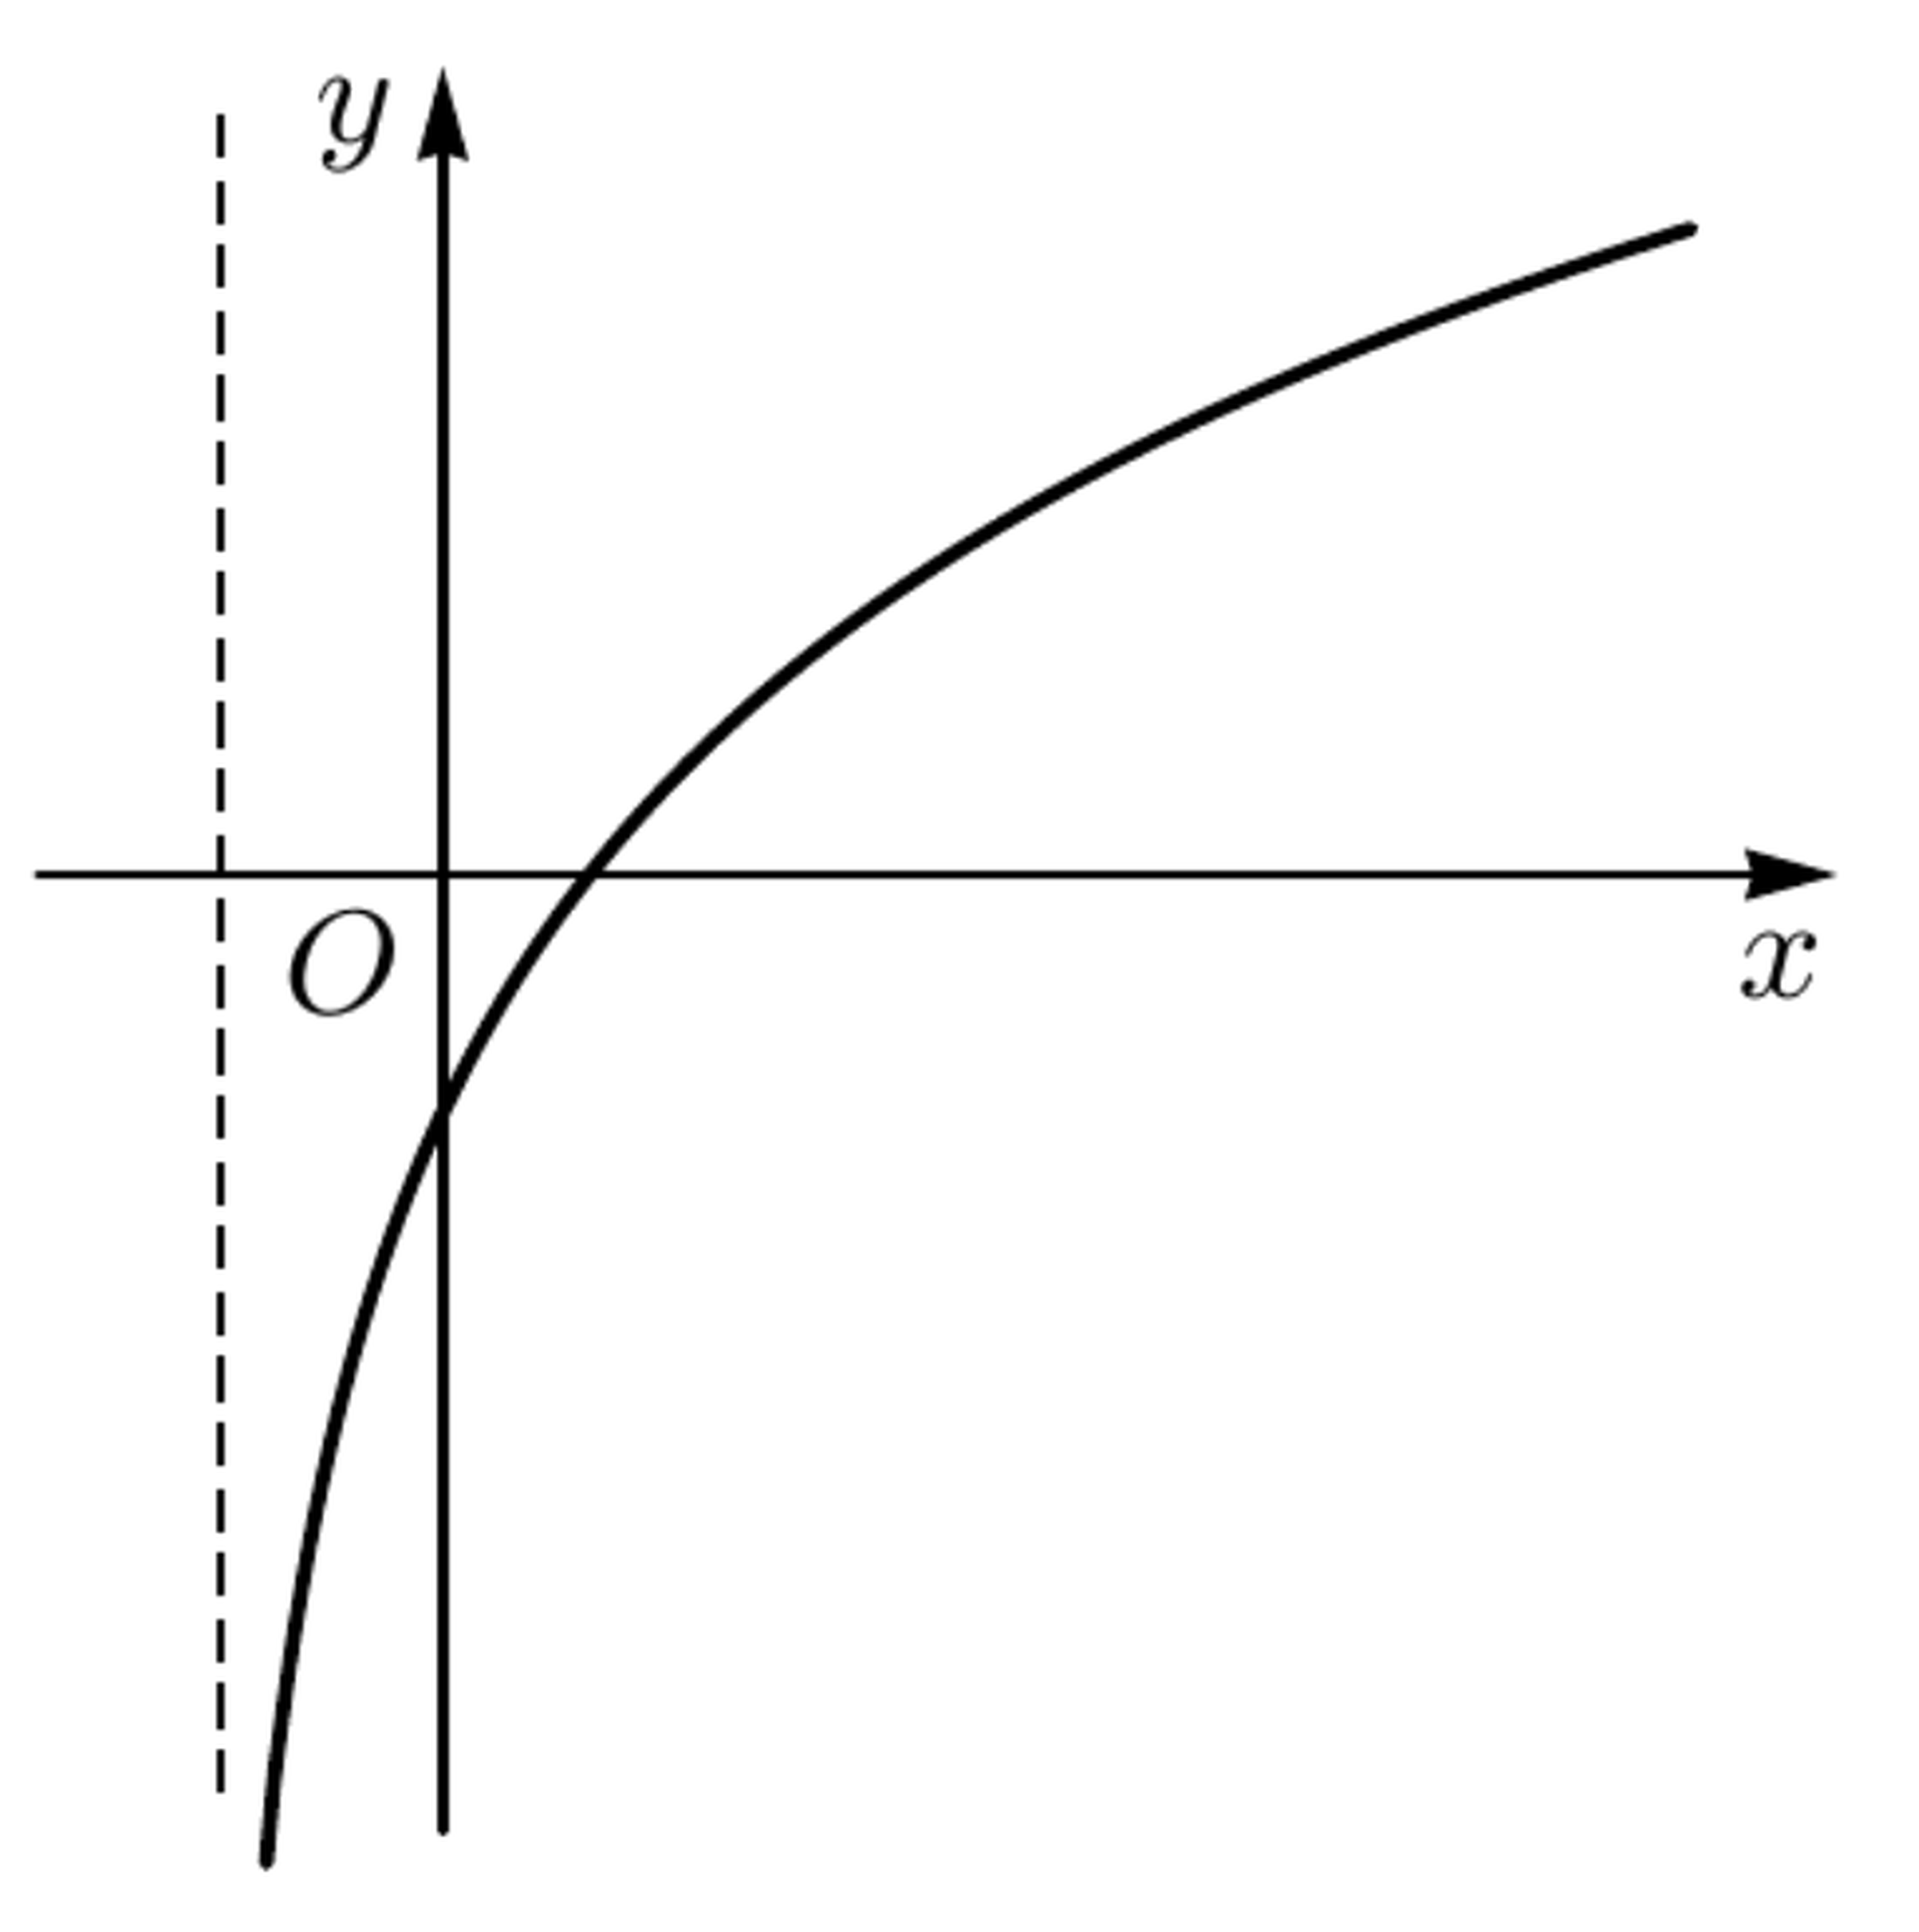
\includegraphics[width=0.42\textwidth]{figures/gao158_q15.png}
\end{center}

\keepwithprev
A. $a>1, b>1$\qquad\qquad B. $a>1, 0<b<1$

C. $0<a<1, b>1$\qquad\qquad D. $0<a<1, 0<b<1$

\ifanswer
\solbegin
\step{图像严格增，得 $a>1$.}
\step{图像与 $y$ 轴交于 $x$ 轴下方，得 $b>0$ 且 $\log_a b<0$，即 $0<b<1$，故选 $B$.}
\solend
\fi

% === Q16 === \lvert\log_2 x\rvert；解析 5 行，故选 C
\item 已知函数 $f(x)=\lvert\log_2 x\rvert$，若 $0<a<b$ 且 $f(a)=f(b)$，则 $a+2b$ 的取值范围是\mbox{（\quad）}

\keepwithprev
A. $(2\sqrt2,+\infty)$\qquad B. $[2\sqrt2,+\infty)$\qquad C. $(3,+\infty)$\qquad D. $[3,+\infty)$

\ifanswer
\solbegin
\step{由 $a<b$ 及 $\lvert\log_2 a\rvert=\lvert\log_2 b\rvert$，得 $\log_2 a=-\log_2 b$，即 $ab=1$，}
\step{且 $0<a<1<b$.}
\step{设 $t=a+2b=2b+\dfrac1b$，则 $t-3=\dfrac{(b-1)(2b-1)}{b}>0$.}
\step{反之，任取 $t>3$，令 $b=\dfrac{t+\sqrt{t^2-8}}{4}>1$、$a=\dfrac1b$，则满足题设且 $a+2b=t$.}
\step{因此取值范围为 $(3,+\infty)$，故选 $C$.}
\solend
\fi

\end{enumerate}

\bigsec{三、解答题}

\begin{enumerate}
\setcounter{enumi}{16}

% === Q17 === 集合、\overline{A}、\subseteq；解析 9 行
\item 已知全集 $U=\R$，集合 $A=\left\{x\mid\dfrac{x-3}{x+1}\leqslant0\right\}$，$B=\{x\mid x^2-2mx+m^2-9<0\}$（$m$ 为实数）.

(1) 当 $m=4$ 时，求 $A\cap B$ 和 $\overline{A}\cup B$；

(2) 若“$x\in A$”是“$x\in B$”的充分条件，求实数 $m$ 的取值范围.

\ifanswer
\solbegin
\step{(1) $\dfrac{x-3}{x+1}\leqslant0\Leftrightarrow-1<x\leqslant3$，所以 $A=(-1,3]$.}
\step{当 $m=4$ 时，$B=\{x\mid(x-4)^2<9\}=(1,7)$，}
\step{于是 $A\cap B=(1,3]$，$\overline{A}\cup B=(-\infty,-1]\cup(1,+\infty)$；}
\step{(2) $x^2-2mx+m^2-9<0\Leftrightarrow(x-m)^2<9$，所以 $B=(m-3,m+3)$.}
\step{题设充分条件等价于 $A\subseteq B$.}
\step{由于 $A=(-1,3]$，左端须满足 $m-3\leqslant-1$.}
\step{又 $3\in A$，须有 $3<m+3$.}
\step{这两个条件也保证 $(-1,3]\subseteq(m-3,m+3)$，}
\step{因此 $A\subseteq B\Leftrightarrow\begin{cases}m-3\leqslant-1\\m+3>3\end{cases}\Leftrightarrow0<m\leqslant2$.}
\solend
\fi

% === Q18 === 蓄水池造价（含 (3) 场地限制）；单位 \mathrm{m}；解析 13 行
\item 某工厂拟建一个容积为 $400\mathrm{m}^3$ 的无盖长方体蓄水池，池深 $4\mathrm{m}$，池底为矩形，其一边长
为 $x\mathrm{m}$. 池壁每平方米造价 100 元，池底每平方米造价 150 元. 设水池的总造价为 $C$
元.

(1) 把 $C$ 表示成 $x$ 的函数，并写出它的定义域；

(2) 当 $x$ 为何值时，总造价最低？最低造价是多少？

(3) 受场地限制，池底一边长 $x$ 不超过 $8\mathrm{m}$，此时总造价最低是多少？

\ifanswer
\solbegin
\step{(1) 设池底另一边长为 $y\mathrm{m}$，则 $4xy=400$，所以 $y=\dfrac{100}{x}$，$x>0$.}
\step{池底面积为 $100\mathrm{m}^2$，池壁总面积为 $8\left(x+\dfrac{100}{x}\right)\mathrm{m}^2$，}
\step{因此 $C(x)=100\times8\left(x+\dfrac{100}{x}\right)+150\times100=800x+\dfrac{80000}{x}+15000$，}
\step{定义域为 $(0,+\infty)$.}
\step{(2) 因为 $x>0$，所以 $C(x)=800\left(x+\dfrac{100}{x}\right)+15000$，}
\step{$\geqslant800\times2\sqrt{x\cdot\dfrac{100}{x}}+15000=31000$，}
\step{当且仅当 $x=\dfrac{100}{x}$，即 $x=10$ 时取等号.}
\step{答：当 $x=10$ 时，总造价最低，为 31000 元.}
\step{(3) 此时定义域为 $(0,8]$. 任取 $0<x_1<x_2\leqslant8$，}
\step{则 $C(x_2)-C(x_1)=800(x_2-x_1)\left(1-\dfrac{100}{x_1x_2}\right)<0$，}
\step{所以 $C(x)$ 在 $(0,8]$ 上严格递减，$x=8$ 时总造价最低，}
\step{且 $C(8)=800\times8+\dfrac{80000}{8}+15000=31400$.}
\step{答：受场地限制时，最低总造价为 31400 元.}
\solend
\fi

% === Q19 === 甲乙滤材 0.8^n／0.7^n；解析 17 行
\item 某环保公司研发了两种新型滤材甲和乙：污水每经过一层甲滤材，污染物含量减少
20\%；每经过一层乙滤材，污染物含量减少 30\%. 每层甲滤材成本 3 万元，每层乙滤材
成本 4 万元. 设原污水中污染物含量为 1，要求处理后污染物含量低于原来的 5\%.

(1) 若只使用一种滤材，污水经过 $n$ 层后污染物含量为 $y$，分别写出使用甲、乙两种滤材
时 $y$ 关于 $n$ 的函数关系式（$n$ 为正整数）；

(2) 若只使用一种滤材，分别求甲、乙至少各需要多少层，并比较哪种滤材的总成本更
低；

(3) 若两种滤材可以混合使用（先后顺序不影响效果），设使用甲滤材 $m$ 层、乙滤材 $n$
层（$m$、$n$ 为非负整数），求满足要求的最低总成本，并指出此时 $m$、$n$ 的值.

\ifanswer
\solbegin
\step{(1) 甲：$y=0.8^n$；乙：$y=0.7^n$，其中 $n$ 为正整数.}
\step{(2) 两种滤材均须满足 $y<0.05$，且污染物含量随层数增加而严格减少.}
\step{$0.8^{14}\approx0.04398<0.05<0.05498\approx0.8^{13}$，}
\step{$0.7^9=0.040353607<0.05<0.05764801=0.7^8$，}
\step{甲至少需要 14 层，成本为 $3\times14=42$ 万元；}
\step{乙至少需要 9 层，成本为 $4\times9=36$ 万元.}
\step{因此，只使用一种滤材时，使用乙滤材的总成本更低.}
\step{(3) 设总成本为 $C$ 万元，则 $C=3m+4n,0.8^m\cdot0.7^n<0.05,m,n\in\{0,1,2,\cdots\}$，}
\step{若 $m\geqslant3$，将其中 3 层甲替换为 2 层乙，}
\step{因为 $0.7^2=0.49<0.512=0.8^3,2\times4<3\times3$，}
\step{替换后污染物含量更低，成本减少 1 万元，因此最低成本方案必有 $m\leqslant2$.}
\step{当 $m=0$ 时，由第（2）小题得至少需要 9 层乙，最低成本为 36 万元.}
\step{当 $m=1$ 或 $m=2$ 时，$0.8\cdot0.7^7>0.8^2\cdot0.7^7=0.052706752>0.05$，}
\step{$0.8^2\cdot0.7^8<0.8\cdot0.7^8=0.046118408<0.05$，}
\step{因此两种情形均至少需要 8 层乙，}
\step{对应最低成本分别为 $3+4\times8=35$ 万元，$3\times2+4\times8=38$ 万元.}
\step{答：满足要求的最低总成本为 35 万元，此时使用甲滤材 1 层、乙滤材 8 层.}
\solend
\fi

% === Q20 === f(x)=\log_2(4^x+1)-x；\Delta；解析 17 行
\item 已知函数 $f(x)=\log_2(4^x+1)-x$.

(1) 证明 $f(x)=\log_2(2^x+2^{-x})$，并求 $f(x)$ 的最小值及取得最小值时 $x$ 的值；

(2) 解不等式 $f(x)>\log_2 5-1$；

(3) 证明：函数 $f(x)$ 在区间 $[0,+\infty)$ 上是严格增函数；并求使关于 $x$ 的方程 $f(x)=m$ 恰
有两个不同实数解的实数 $m$ 的取值范围.

\ifanswer
\solbegin
\step{(1) $f(x)=\log_2(4^x+1)-\log_2 2^x=\log_2\dfrac{4^x+1}{2^x}=\log_2(2^x+2^{-x})$，}
\step{因为 $2^x+2^{-x}\geqslant2\sqrt{2^x\cdot2^{-x}}=2$，所以 $f(x)\geqslant\log_2 2=1$，}
\step{等号当且仅当 $2^x=2^{-x}$，即 $x=0$ 时成立，故最小值为 1.}
\step{(2) 令 $t=2^x>0$，则 $f(x)>\log_2 5-1\Leftrightarrow t+\dfrac1t>\dfrac52\Leftrightarrow2t^2-5t+2>0$}
\step{$\Leftrightarrow(2t-1)(t-2)>0$，}
\step{结合 $t>0$，得 $0<t<\dfrac12$ 或 $t>2$，即 $x<-1$ 或 $x>1$，}
\step{解集为 $(-\infty,-1)\cup(1,+\infty)$.}
\step{(3) 任取 $0\leqslant x_1<x_2$，记 $a=2^{x_1}$，$b=2^{x_2}$，则 $1\leqslant a<b$，$ab>1$，}
\step{从而 $\left(b+\dfrac1b\right)-\left(a+\dfrac1a\right)=(b-a)\left(1-\dfrac{1}{ab}\right)>0$，}
\step{由对数函数的严格递增性，得 $f(x_1)<f(x_2)$，}
\step{所以 $f(x)$ 在 $[0,+\infty)$ 上是严格增函数.}
\step{当 $m<1$ 时，由（1）得方程无实数解；当 $m=1$ 时，只有实数解 $x=0$.}
\step{当 $m>1$ 时，令 $t=2^x>0$，则 $f(x)=m\Leftrightarrow t+\dfrac1t=2^m\Leftrightarrow t^2-2^m t+1=0$，}
\step{此时 $\Delta=2^{2m}-4>0$，两根之和为 $2^m>0$、之积为 $1>0$，}
\step{故有两个不同的正根.}
\step{每个正根 $t$ 唯一确定一个实数 $x=\log_2 t$，故原方程恰有两个不同实数解，}
\step{所求范围为 $m\in(1,+\infty)$.}
\solend
\fi

% === Q21 === f(x)=4^x-m\cdot2^{x+1}+3 值域与 h(m) 分段；解析 13 行
\item 已知函数 $f(x)=4^x-m\cdot2^{x+1}+3$（$m\in\R$），$x\in[0,2]$.

(1) 当 $m=1$ 时，求 $f(x)$ 的值域；

(2) 记 $f(x)$ 的最小值为 $h(m)$，求 $h(m)$ 的表达式；

(3) 若关于 $x$ 的方程 $f(x)=0$ 在区间 $[0,2]$ 上有解，求实数 $m$ 的取值范围.

\ifanswer
\solbegin
\step{令 $t=2^x$，则 $t\in[1,4]$，且 $f(x)=t^2-2mt+3=(t-m)^2+3-m^2$，}
\step{(1) 当 $m=1$ 时，$f(x)=(t-1)^2+2$.}
\step{由 $0\leqslant t-1\leqslant3$，得 $2\leqslant f(x)\leqslant11$，值域为 $[2,11]$.}
\step{(2) 二次函数 $y=(t-m)^2+3-m^2$ 的对称轴为直线 $t=m$.}
\step{当 $m\leqslant1$ 时，在 $t=1$ 处取最小值；}
\step{当 $1<m<4$ 时，在 $t=m$ 处取最小值；}
\step{当 $m\geqslant4$ 时，在 $t=4$ 处取最小值；}
\step{因此 $h(m)=\begin{cases}4-2m,&m\leqslant1\\3-m^2,&1<m<4\\19-8m,&m\geqslant4\end{cases}$；}
\step{(3) 方程 $f(x)=0$ 在 $[0,2]$ 上有解，}
\step{等价于存在 $t\in[1,4]$，使 $m=\dfrac{t^2+3}{2t}=\dfrac12\left(t+\dfrac3t\right)$，}
\step{由基本不等式，$m\geqslant\dfrac12\cdot2\sqrt{t\cdot\dfrac3t}=\sqrt3$，当且仅当 $t=\sqrt3$ 时取等号；}
\step{又 $\dfrac{19}{8}-m=\dfrac{(4-t)(4t-3)}{8t}\geqslant0$，当且仅当 $t=4$ 时取等号；}
\step{因此必有 $\sqrt3\leqslant m\leqslant\dfrac{19}{8}$.}
\solend
\fi

\end{enumerate}

\end{document}
"
%
% ① 原始材料：微信公众号"魔都数学加油站"文章，连载"27学年高一158"，原文标题
% "27学年高一158——2026-2027年上海市上实东滩高一上期中"（本卷本地编号 158 与
% 原卷连载号一致，无撞号）。
% 正文为 9 张 PNG 页（01/05/08/09 为 2560×3620，02/03/04/06/07 为 4762×6735，
% 同一篇各页分辨率混排，逐页按各自分辨率裁图核对）。
% 体例：讲评版——填空 3—12（10 题）、选择 13—16（4 题）、解答 17—21（5 题），
% 共 19 题，自第 3 题起编（1、2 未印在本篇）；Q5 只印【答案】、其余 18 题
% 逐题印【解析】（逐题核实，见 ②）。题目、答案、解析均据原图转录；卷面粉红色
% 水印"魔都数学加油站"及公众号页脚未录入。全卷末题为第 21 题，无附加题节。
% 全卷 2 组配图（逐页通读 9 页确认）——
%   · Q10 题干右侧"曼 → man"字形变换图（02 页），题目配图、三版都出，
%     裁 figures/gao158_q10.png；
%   · Q15 题干"如图所示"对数函数大致图像（03 页右下），题目配图、三版都出，
%     裁 figures/gao158_q15.png；
% 2 图均取自原卷截图，去粉色水印、转灰度、4× LANCZOS 放大；
% 其余各页逐页确认无其它题目配图、无解析内配图、无表格。
%
% 卷首标题：原卷印作"2026-2027 年上实东滩高一上期中"，年份区间按全稿惯例排 en dash；
% 原卷卷面未印副标题，本稿按同期中卷知识模块口径补出"集合与常用逻辑用语、不等式、函数"。
%
% ② 与原卷的排版差异／照录项清单：
%   ① 原文从第 3 题起，本稿保留原题号；共 19 题三节，解答题 5 题到 21；
%      三节各自一个 enumerate＋各自 \setcounter{enumi}{2}／{12}／{16}，
%      不贯穿（题目溯源.py 按 \bigsec 切节、每节独立计 depth，只收 depth==1 的 \item）；
%   ② 混合体例：Q5 只印【答案】、无【解析】，按 高一156 第 3 题成例另提
%      \ans{}、不补造解析；其余 18 题印【解析】、用 \solbegin…\solend；
%      四道选择题答案均在解析末句"故选 C／B／B／C"（逐个放大复核）、
%      题干括号 \mbox{（\quad）} 留空、不另提 \ans{}；答案版
%      【答案】/【解析】标记数 = 19 = 全卷题数（1 个 \ans ＋ 18 个 \solbegin）；
%   ③ 原卷卷面未印副标题，本稿按知识模块口径补出；
%   ④ 原卷填空横线按全稿惯例排 \blankline[4.4em]；选择题选项段前按惯例各加
%      \keepwithprev；解答题不留作答区、不加 \anspace（原卷为讲评版）；
%   ⑤ 数集：Q13"在 \R 上严格递增"、Q14"$x\in\R$"、Q17"$U=\R$"、
%      Q21"$m\in\R$" 原卷印正体粗体 R，按全稿惯例归一 \R；
%      绝对值排 \lvert…\rvert（Q12 $\lvert a\rvert$、Q14 $\lvert x-2\rvert$、
%      Q16 $\lvert\log_2 x\rvert$／$\lvert\log_2 a\rvert$／$\lvert\log_2 b\rvert$），
%      集合描述竖线排 \mid（Q17），不等号按全稿惯例排 \leqslant／\geqslant，
%      补集上划线 \overline{A}（Q17）；
%   ⑥ 子集／真子集符号逐处照录不统一：Q14 解析"$(2,3)\subsetneq(1,3)$"原卷印
%      带下划线且被斜杠划过的 ⊊（真子集，放大 03 页确认），照录 \subsetneq；
%      Q17 解析三处"$A\subseteq B$""$(-1,3]\subseteq(m-3,m+3)$"原卷印
%      带下划线 ⊆（放大 05 页确认），照录 \subseteq；本卷无单线 \subset 用例；
%   ⑦ 判别式：Q20 (3) 解析"$\Delta=2^{2m}-4>0$"原卷印高瘦等腰 \Delta
%      （像素实测高/宽 ≈ 1.13，扁三角 \triangle 为 0.93，放大 08 页确认），
%      照录 \Delta；本卷无扁三角 \triangle 用例；
%   ⑧ "图像"与"图象"：全卷统一用"图像"（Q6 题干、Q10 两处、Q11 解析、
%      Q15 题干与解析两处，逐处放大确认带单人旁），照录不改；
%   ⑨ 中文弯引号照录：Q5 命题"若实数…"、Q10"曼""man""新"、Q14 题干与
%      解析的两则不等式、Q17 (2)"$x\in A$""$x\in B$"；注释里一律 ASCII 引号；
%   ⑩ 半角逗号逐处照录：Q8"$2,3,4$""$-2,-1,0$"、Q10 点坐标 $(x,y)$／
%      $(t,2^t-1)$／$(1-2^t,t)$、Q15 四选项"$a>1, b>1$"等、
%      Q19 (3)"$C=3m+4n,0.8^m\cdot0.7^n<0.05,m,n\in\{0,1,2,\cdots\}$"
%      与"$0.7^2=0.49<0.512=0.8^3,2\times4<3\times3$"、
%      Q21 cases 内"$4-2m,$"等；其余行中逗号／顿号照录全角；
%      行末西文句点 ASCII `.`；
%   ⑪ 顿号照录：Q3"（用 $a$、$b$ 表示）"、Q5"$x$、$y$"、Q13"A、B"、
%      Q16 解析"$>1$、$a=\dfrac1b$"、Q19"甲、乙""$m$、$n$"、
%      Q20"$2^m>0$、之积为"、Q21"$m$、$n$"；顿号一律移到数学模式外，
%      数学模式内不出现中文标点；
%   ⑫ 角度与单位照录：Q10 三处"$90^{\circ}$"、Q18"$400\mathrm{m}^3$"
%      "$4\mathrm{m}$""$x\mathrm{m}$""$8\mathrm{m}$""$y\mathrm{m}$"
%      "$100\mathrm{m}^2$""$\left(x+\dfrac{100}{x}\right)\mathrm{m}^2$"；
%      Q19 百分号"20\%""30\%""5\%"按原卷排 \%；
%   ⑬ 文本模式全角括号照录：Q10"（提示：…）"、Q17"（$m$ 为实数）"、
%      Q19"（$n$ 为正整数）""（先后顺序不影响效果）""（$m$、$n$ 为非负整数）"、
%      Q20"由（1）得"、Q19"由第（2）小题"、Q21"（$m\in\R$）"；
%      子题行首标号按全稿惯例用半角 (1)(2)(3)；
%   ⑭ 复杂式照录别简化：Q3 $\dfrac{\log_3 2+\log_3 5}{\log_3 3+2\log_3 2}$、
%      Q8 $[-3,-2)\cup(4,5]$、Q9 $18ab=2^t\cdot3^t=6^t=a+b$、
%      Q12 $\dfrac{\sqrt6}{2}$、Q18 $C(8)=800\times8+\dfrac{80000}{8}+15000=31400$
%      （原卷即 C(8)，非 C(2)）、Q19 $0.8^{14}\approx0.04398$、
%      $0.7^9=0.040353607$、$0.052706752$、$0.046118408$、
%      Q20 $t^2-2^m t+1=0$、Q21 $h(m)$ 三段 cases 与 $\dfrac{(4-t)(4t-3)}{8t}$ 等；
%      \left…\right 不得拆到不同 $…$ 组；cases 块整体算一个印刷行；
%   ⑮ 一条 \step = 原卷解析的一个印刷行；别并折行、别拆行。跨页续印按题合并
%      （Q7 的 01—02 页、Q9/Q10/Q11 的 02—03 页、Q13/Q14 的 03 页上下、
%      Q15/Q16 的 04 页上下、Q17 的 04—05 页、Q18 的 05—06 页、
%      Q19 的 06—07 页、Q20 的 07—08 页、Q21 的 08—09 页）；
%      跨半页重叠行（Q5【答案】、Q9 设公共值行、Q10 题干、Q16 反之行、
%      Q18 (2) 题干、Q19 末两行、Q20 (3) 末行、Q21 cases 块）只算一个印刷行；
%   ⑯ 配图：2 组题目配图（见 ①），均三版都出，\needvspace 守卫放 \item 之前
%      把"题干＋图"整块推走，\includegraphics 放题干之后；本卷无解析内配图、
%      无红字加粗小标题（全卷逐页确认，故无 \stepm）。
%
% ③ 行数复核：一条 \step = 原卷解析的一个印刷行，cases 块作一个印刷行计。
%   逐题数（逐页核对）：Q3：1；Q4：2；Q5：0（只印【答案】、提 \ans{}，
%   不计入 \step 账）；Q6：1；Q7：4；Q8：5；Q9：2；Q10：2；Q11：3；
%   Q12：3；Q13：2；Q14：3；Q15：2；Q16：5；Q17：9；Q18：13；
%   Q19：17；Q20：17；Q21：13。
%   合计 104 行（104 条 \step ＋ 0 条 \stepm），与原卷逐题印刷行相等。
%   全卷 19 题：Q5 一处 \ans{} ＋ 其余 18 题设 \solbegin…\solend，
%   答案版【答案】/【解析】标记数 = 19 = 全卷题数。
%
% ④ 页码分布（供回原图复核）：
%   卷首标题＋"一、填空题"＋Q3 题干＋解析 1 行、Q4 题干＋解析 2 行、
%   Q5 题干＋【答案】在 01 页上半；Q5【答案】（重叠重印）＋Q6 题干＋解析 1 行、
%   Q7 题干＋解析前 3 行在 01 页下半；Q7 解析末行＋Q8 题干＋解析 5 行、
%   Q9 题干＋解析首行在 02 页上半；Q9 解析末行＋Q10 题干（含"曼→man"图）
%   ＋解析 2 行＋Q11 题干＋解析首行在 02 页下半；Q11 解析后 2 行＋Q12 题干
%   ＋解析 3 行＋"二、选择题"标题＋Q13 题干＋选项在 03 页上半；
%   Q13 选项（重叠重印）＋解析 2 行＋Q14 题干＋选项＋解析 3 行＋Q15 题干
%   ＋对数图像（右侧）在 03 页下半；Q15 选项＋解析 2 行＋Q16 题干＋选项
%   ＋解析前 4 行在 04 页上半；Q16 解析末行＋"三、解答题"标题＋Q17 题干
%   ＋两问＋解析 (1) 3 行在 04 页下半；Q17 解析 (2) 6 行＋Q18 题干＋三问
%   ＋解析 (1) 4 行＋(2) 首行在 05 页上下；Q18 解析 (2) 后 3 行＋(3) 5 行
%   ＋Q19 题干＋三问＋解析 (1) 1 行＋(2) 3 行在 06 页上下；Q19 解析 (2) 3 行
%   ＋(3) 12 行在 07 页上半；Q19 解析末 2 行（重叠）＋Q20 题干＋三问
%   ＋解析 (1) 3 行在 07 页下半；Q20 解析 (2) 4 行＋(3) 前 4 行在 08 页上半；
%   Q20 解析 (3) 后 6 行＋Q21 题干＋(1) 问在 08 页下半；Q21 (2)(3) 问＋
%   解析 (1) 3 行＋(2) 5 行＋cases 块在 09 页上半；Q21 cases 块（重叠）
%   ＋(3) 解析 5 行在 09 页下半。本稿按题连排，不丢行、不并折行；
%   全卷末题为第 21 题，无附加题节。
%
% ⑤ 存疑／需主会话回原图复核：
%   1. Q14 解析"$(2,3)\subsetneq(1,3)$"的 ⊊（真子集带斜杠）与 Q17 的 ⊆
%      是两种不同记号，本稿分别照录 \subsetneq／\subseteq，请复核；
%   2. Q20 (3)"$\Delta=2^{2m}-4>0$"判为高瘦 \Delta，请复核是否 \triangle；
%   3. 任务书提示"Q18 解析里印 C(2)=…"，但 06 页原图逐处读作
%      $C(8)=800\times8+\dfrac{80000}{8}+15000=31400$，未找到 C(2)，
%      本稿照原卷排 C(8)，请复核；
%   4. Q19 解析末句"最低总成本为 35 万元"（07 页上下两处印同），
%      OCR 曾误读为 34，本稿按 35 照录，请复核；
%   5. Q10 提示末尾"坐标为 $(-y,x)$）."为半角 $)$＋全角 $）$ 两枚括号，
%      本稿照录，请复核；
%   6. Q21 cases 块后"；"落在分式中行右侧（排版居中基线所致），
%      本稿排作 $…\end{cases}$；，请复核。
%   全卷除此 6 类外未发现其它笔误／自相矛盾处；19 题中 18 题印【解析】。
%
\documentclass[a4paper,11pt]{article}
\usepackage{common}

\begin{document}

\examtitlest[3]{2026--2027 年上实东滩高一上期中}{集合与常用逻辑用语、不等式、函数}

\bigsec{一、填空题}

\begin{enumerate}
\setcounter{enumi}{2}

% === Q3 === 换底公式；解析 1 行
\item 已知 $3^a=5$，$\log_3 2=b$，则 $\log_{12} 10=$\blankline[4.4em]（用 $a$、$b$ 表示）.

\ifanswer
\solbegin
\step{$\log_{12} 10=\dfrac{\log_3 2+\log_3 5}{\log_3 3+2\log_3 2}=\dfrac{a+b}{1+2b}$.}
\solend
\fi

% === Q4 === 定义域；解析 2 行；半角括号 ( ) 与全角逗号照录
\item 函数 $y=\sqrt{2-x}+\lg(x^2-1)$ 的定义域为\blankline[4.4em].

\ifanswer
\solbegin
\step{由 $2-x\geqslant0$ 且 $x^2-1>0$，得 $x\leqslant2$ 且 ($x<-1$或$x>1$)，}
\step{定义域为 $(-\infty,-1)\cup(1,2]$.}
\solend
\fi

% === Q5 === 只印【答案】、无【解析】；反证法，中文弯引号
\item 用反证法证明命题“若实数 $x$、$y$ 满足 $x+y>2$，则 $x$、$y$ 中至少有一个大于 1”时，
应假设\blankline[4.4em].

\ifanswer
\ans{$x\leqslant1$ 且 $y\leqslant1$}
\fi

% === Q6 === 图像平移；解析 1 行
\item 函数 $y=\dfrac{2x+1}{x-1}$ 的图像可由函数 $y=\dfrac{3}{x}$ 的图像先向右平移 $a$ 个单位，再向上平移 $b$ 个单位
得到，则 $a+b=$\blankline[4.4em].

\ifanswer
\solbegin
\step{$y=\dfrac{2x+1}{x-1}=\dfrac{3}{x-1}+2$，所以 $a=1$，$b=2$，$a+b=3$.}
\solend
\fi

% === Q7 === 集合三元子集；解析 4 行，跨 01—02 页
\item 设 $A=\{a_1,a_2,a_3,a_4\}$ 是由四个实数组成的集合，若 $A$ 的所有三元子集中，三个元素之和
组成的集合为 $B=\{1,4,7,12\}$，则集合 $A=$\blankline[4.4em].

\ifanswer
\solbegin
\step{设 $S=a_1+a_2+a_3+a_4$，}
\step{每个元素在四个三元子集中恰出现三次，则 $3S=1+4+7+12=24$，得 $S=8$.}
\step{四个三元子集的元素和分别为 $S-a_i$，}
\step{所以 $A=\{8-1,8-4,8-7,8-12\}=\{-4,1,4,7\}$.}
\solend
\fi

% === Q8 === 不等式整数解；解析 5 行；半角逗号照录
\item 不等式 $x^2-(a+1)x+a<0$ 的解集中恰有 3 个整数，则 $a$ 的取值范围是\blankline[4.4em].

\ifanswer
\solbegin
\step{原不等式为 $(x-1)(x-a)<0$；}
\step{$a=1$ 时解集为空集，不符合题意.}
\step{若 $a>1$，解集为 $(1,a)$，恰含整数 $2,3,4$，则 $4<a\leqslant5$.}
\step{若 $a<1$，解集为 $(a,1)$，恰含整数 $-2,-1,0$，则 $-3\leqslant a<-2$.}
\step{故 $a$ 的取值范围是 $[-3,-2)\cup(4,5]$.}
\solend
\fi

% === Q9 === 对数换底＋指数；解析 2 行
\item 已知正数 $a$、$b$ 满足 $1+\log_2 a=2+\log_3 b=\log_6(a+b)$，则 $\dfrac1a+\dfrac1b=$\blankline[4.4em].

\ifanswer
\solbegin
\step{设公共值为 $t$，则 $2a=2^t$，$9b=3^t$，$a+b=6^t$，}
\step{于是 $18ab=2^t\cdot3^t=6^t=a+b$，即 $\dfrac1a+\dfrac1b=\dfrac{a+b}{ab}=18$.}
\solend
\fi

% === Q10 === "曼"字旋转 90°；题目配图（三版都出）；解析 2 行
\needvspace{6cm}
\item 网上流传一个有趣的字形变换：把汉字“曼”的右半部分旋转 $90^{\circ}$，就得到英文单词
“man”的艺术字. 数学中，把曲线绕原点旋转也会得到“新”的曲线：将函数
$y=2^x-1$ 的图像绕坐标原点 $O$ 逆时针旋转 $90^{\circ}$，得到的曲线恰是某个函数的
图像，则这个函数的解析式为\blankline[4.4em]（提示：点 $(x,y)$ 绕 $O$ 逆时针旋转 $90^{\circ}$ 后的
坐标为 $(-y,x)$）.

\begin{center}

\includegraphics[width=0.42\textwidth]{figures/gao158_q10.png}
\end{center}

\ifanswer
\solbegin
\step{原图像上的点 $(t,2^t-1)$ 旋转后为 $(1-2^t,t)$.}
\step{记其为 $(x,y)$，则 $x=1-2^y$，即 $y=\log_2(1-x)$，定义域为 $(-\infty,1)$.}
\solend
\fi

% === Q11 === 值域；解析 3 行，跨 02—03 页
\item 函数 $f(x)=\sqrt{x-2}-\sqrt{15-3x}$ 的值域为\blankline[4.4em].

\ifanswer
\solbegin
\step{由 $x-2\geqslant0$ 且 $15-3x\geqslant0$，得定义域为 $[2,5]$.}
\step{在 $[2,5]$ 上，$\sqrt{x-2}$ 与 $-\sqrt{15-3x}$ 均严格递增，因此 $f(x)$ 严格递增.}
\step{$f(2)=-3$，$f(5)=\sqrt3$，结合函数的图像，值域为 $[-3,\sqrt3]$.}
\solend
\fi

% === Q12 === 绝对值 \lvert…\rvert；解析 3 行
\item 设实数 $a$ 满足 $a<4a^3-5a<\lvert a\rvert$，则 $a$ 的取值范围是\blankline[4.4em].

\ifanswer
\solbegin
\step{由 $a<\lvert a\rvert$ 得 $a<0$，原不等式为 $a<4a^3-5a<-a$.}
\step{同除以 $a<0$，得 $1>4a^2-5>-1\Leftrightarrow1<a^2<\dfrac32$，结合 $a<0$，}
\step{得 $-\dfrac{\sqrt6}{2}<a<-1$，故解集为 $\left(-\dfrac{\sqrt6}{2},-1\right)$.}
\solend
\fi

\end{enumerate}

\bigsec{二、选择题}

\begin{enumerate}
\setcounter{enumi}{12}

% === Q13 === \R 归一；解析 2 行，故选 C
\item 已知 $a>b$，则下列不等式一定成立的是\mbox{（\quad）}

\keepwithprev
A. $\dfrac1a<\dfrac1b$\qquad B. $a^2>b^2$\qquad C. $a^3>b^3$\qquad D. $ac^2>bc^2$

\ifanswer
\solbegin
\step{幂函数 $y=x^3$ 在 $\R$ 上严格递增，$a>b\Rightarrow a^3>b^3$，C 正确.}
\step{取 $a=1$，$b=-1$ 得 A、B 不成立；取 $c=0$ 得 D 不成立；故选 $C$.}
\solend
\fi

% === Q14 === \subsetneq 真子集；解析 3 行，故选 B
\item 设 $x\in\R$，则“$\lvert x-2\rvert<1$”是“$x^2-5x+6<0$”的\mbox{（\quad）}

\keepwithprev
A. 充分非必要条件\qquad\qquad B. 必要非充分条件

C. 充要条件\qquad\qquad D. 既非充分又非必要条件

\ifanswer
\solbegin
\step{$\lvert x-2\rvert<1\Leftrightarrow1<x<3$，$x^2-5x+6<0\Leftrightarrow(x-2)(x-3)<0\Leftrightarrow2<x<3$.}
\step{由 $(2,3)\subsetneq(1,3)$，得“$\lvert x-2\rvert<1$”是“$x^2-5x+6<0$”的必要非充分条件，}
\step{故选 $B$.}
\solend
\fi

% === Q15 === 对数函数大致图像（题目配图，三版都出）；解析 2 行，故选 B
\needvspace{9cm}
\item 已知函数 $f(x)=\log_a(x+b)$（$a>0$ 且 $a\ne1$）的大致图像如图所示，则 $a$、$b$ 满足
的关系是\mbox{（\quad）}

\begin{center}
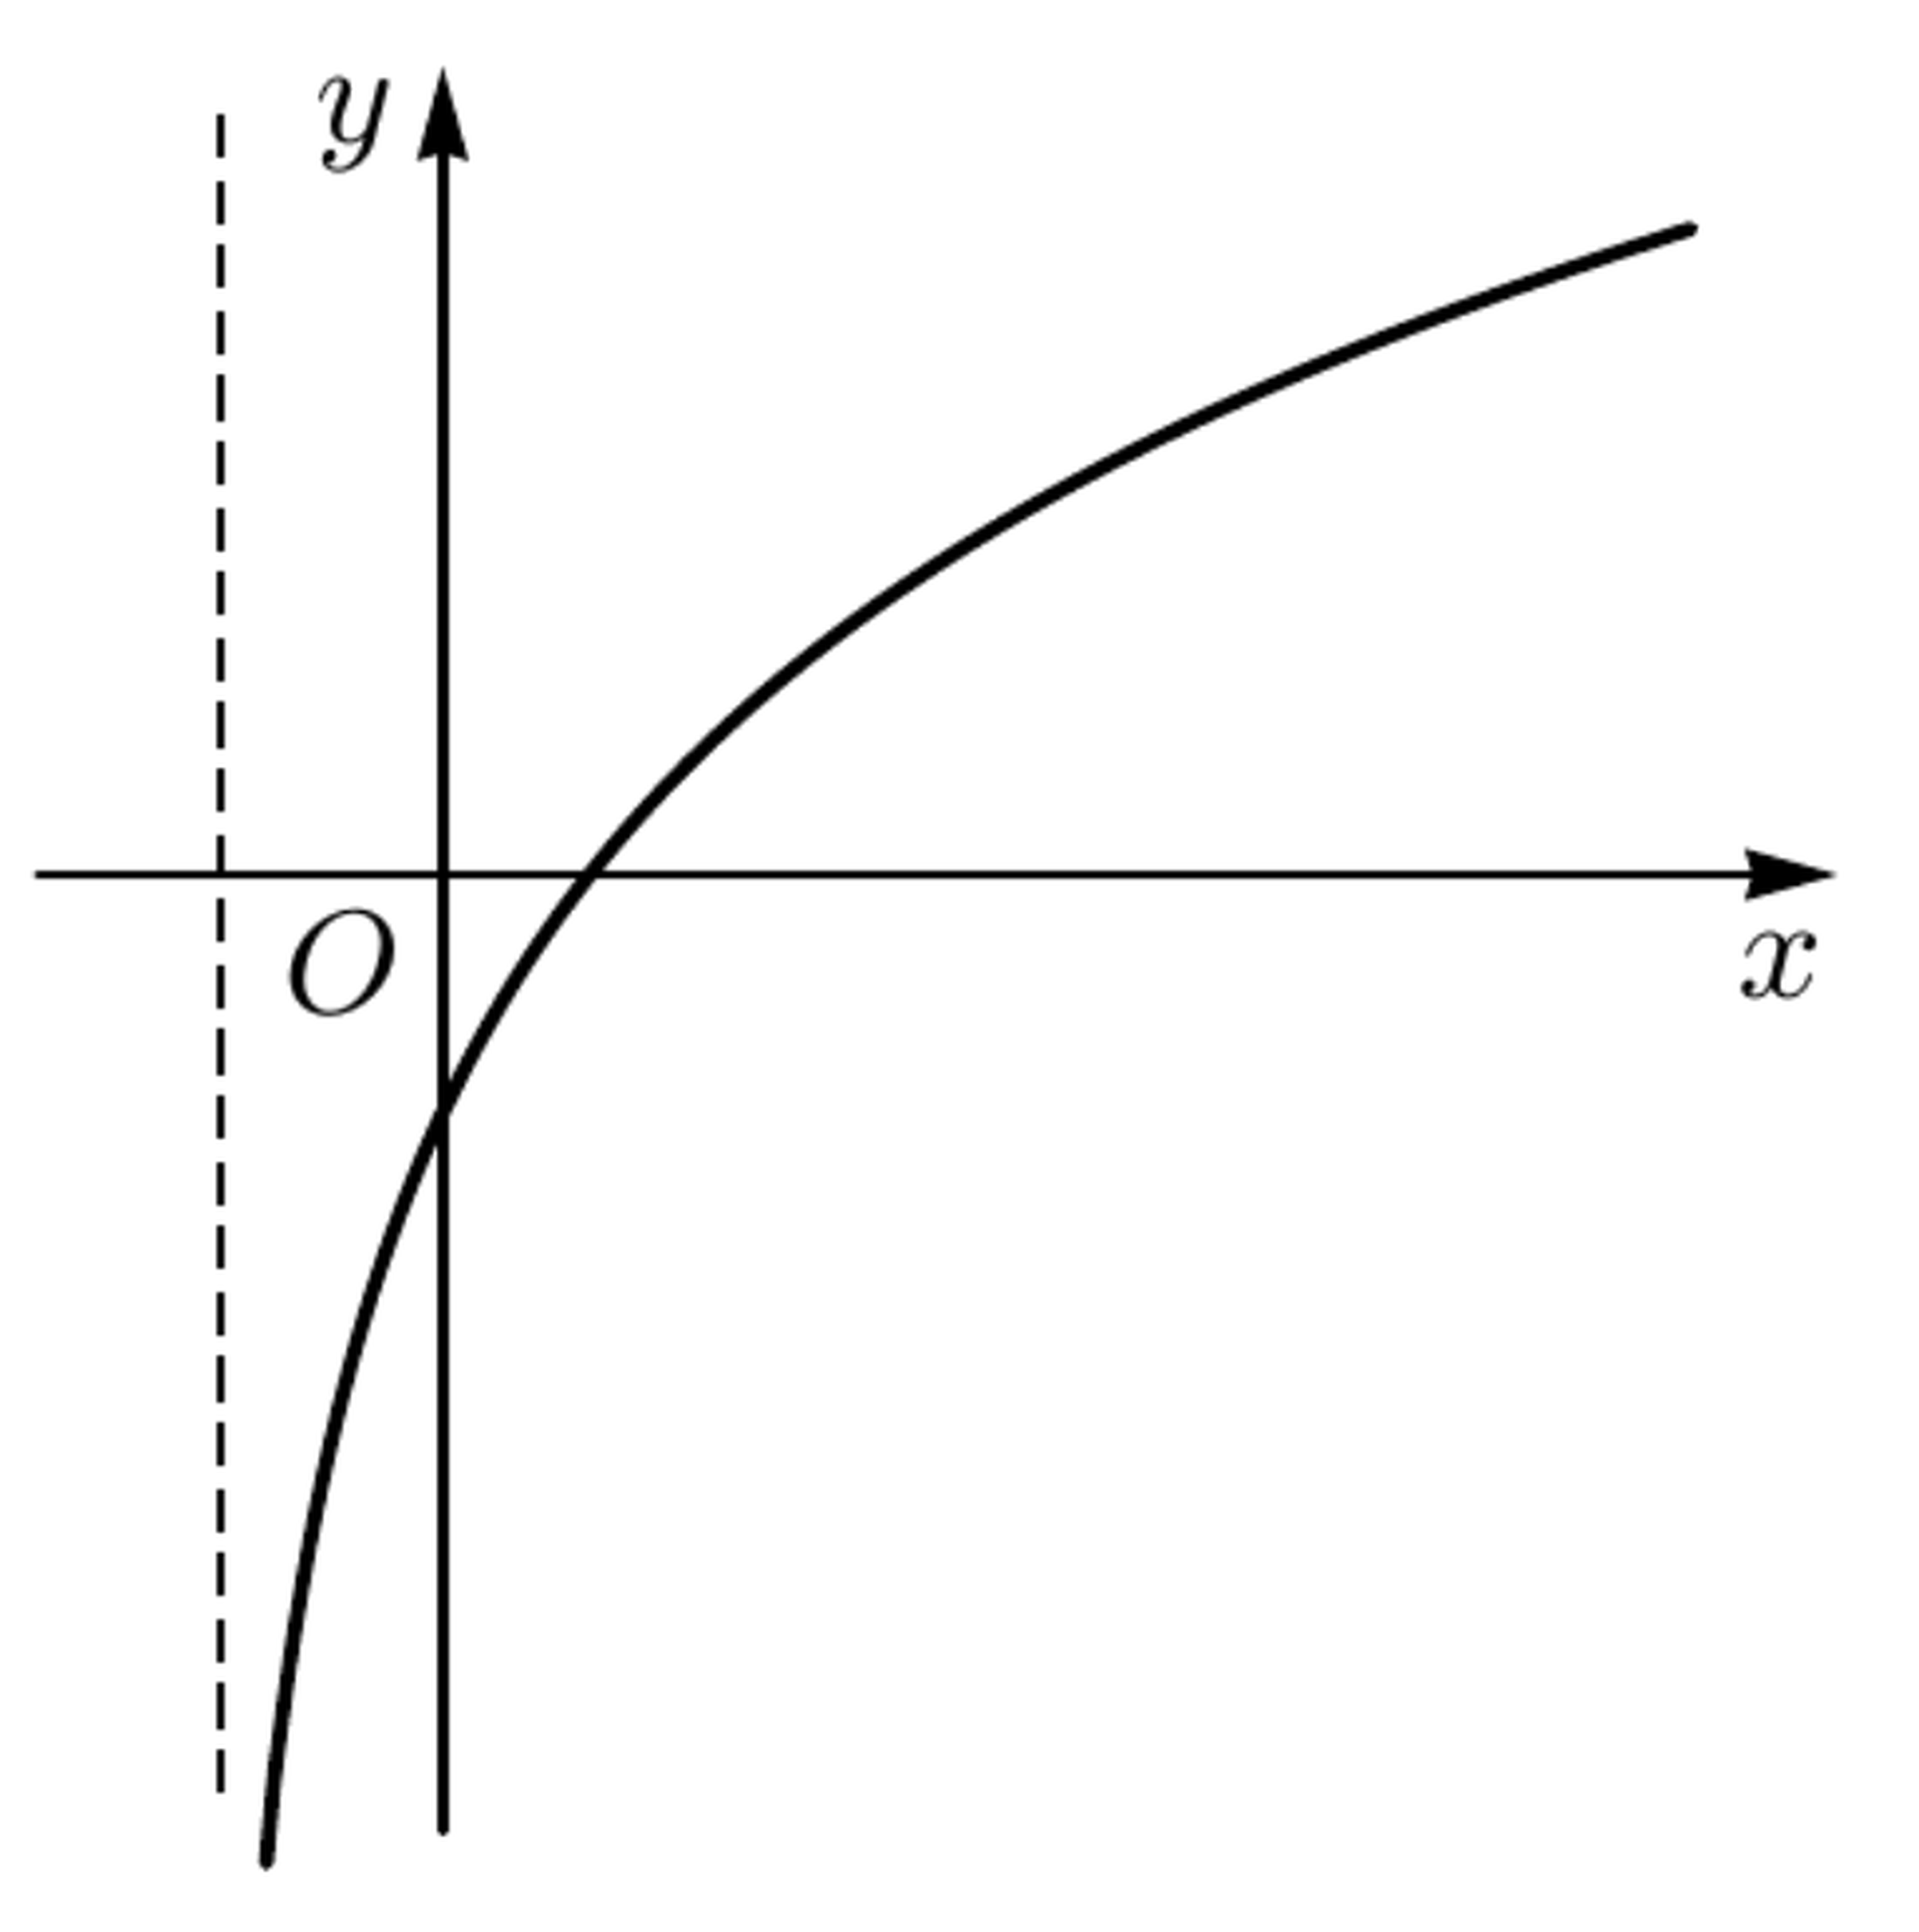
\includegraphics[width=0.42\textwidth]{figures/gao158_q15.png}
\end{center}

\keepwithprev
A. $a>1, b>1$\qquad\qquad B. $a>1, 0<b<1$

C. $0<a<1, b>1$\qquad\qquad D. $0<a<1, 0<b<1$

\ifanswer
\solbegin
\step{图像严格增，得 $a>1$.}
\step{图像与 $y$ 轴交于 $x$ 轴下方，得 $b>0$ 且 $\log_a b<0$，即 $0<b<1$，故选 $B$.}
\solend
\fi

% === Q16 === \lvert\log_2 x\rvert；解析 5 行，故选 C
\item 已知函数 $f(x)=\lvert\log_2 x\rvert$，若 $0<a<b$ 且 $f(a)=f(b)$，则 $a+2b$ 的取值范围是\mbox{（\quad）}

\keepwithprev
A. $(2\sqrt2,+\infty)$\qquad B. $[2\sqrt2,+\infty)$\qquad C. $(3,+\infty)$\qquad D. $[3,+\infty)$

\ifanswer
\solbegin
\step{由 $a<b$ 及 $\lvert\log_2 a\rvert=\lvert\log_2 b\rvert$，得 $\log_2 a=-\log_2 b$，即 $ab=1$，}
\step{且 $0<a<1<b$.}
\step{设 $t=a+2b=2b+\dfrac1b$，则 $t-3=\dfrac{(b-1)(2b-1)}{b}>0$.}
\step{反之，任取 $t>3$，令 $b=\dfrac{t+\sqrt{t^2-8}}{4}>1$、$a=\dfrac1b$，则满足题设且 $a+2b=t$.}
\step{因此取值范围为 $(3,+\infty)$，故选 $C$.}
\solend
\fi

\end{enumerate}

\bigsec{三、解答题}

\begin{enumerate}
\setcounter{enumi}{16}

% === Q17 === 集合、\overline{A}、\subseteq；解析 9 行
\item 已知全集 $U=\R$，集合 $A=\left\{x\mid\dfrac{x-3}{x+1}\leqslant0\right\}$，$B=\{x\mid x^2-2mx+m^2-9<0\}$（$m$ 为实数）.

(1) 当 $m=4$ 时，求 $A\cap B$ 和 $\overline{A}\cup B$；

(2) 若“$x\in A$”是“$x\in B$”的充分条件，求实数 $m$ 的取值范围.

\ifanswer
\solbegin
\step{(1) $\dfrac{x-3}{x+1}\leqslant0\Leftrightarrow-1<x\leqslant3$，所以 $A=(-1,3]$.}
\step{当 $m=4$ 时，$B=\{x\mid(x-4)^2<9\}=(1,7)$，}
\step{于是 $A\cap B=(1,3]$，$\overline{A}\cup B=(-\infty,-1]\cup(1,+\infty)$；}
\step{(2) $x^2-2mx+m^2-9<0\Leftrightarrow(x-m)^2<9$，所以 $B=(m-3,m+3)$.}
\step{题设充分条件等价于 $A\subseteq B$.}
\step{由于 $A=(-1,3]$，左端须满足 $m-3\leqslant-1$.}
\step{又 $3\in A$，须有 $3<m+3$.}
\step{这两个条件也保证 $(-1,3]\subseteq(m-3,m+3)$，}
\step{因此 $A\subseteq B\Leftrightarrow\begin{cases}m-3\leqslant-1\\m+3>3\end{cases}\Leftrightarrow0<m\leqslant2$.}
\solend
\fi

% === Q18 === 蓄水池造价（含 (3) 场地限制）；单位 \mathrm{m}；解析 13 行
\item 某工厂拟建一个容积为 $400\mathrm{m}^3$ 的无盖长方体蓄水池，池深 $4\mathrm{m}$，池底为矩形，其一边长
为 $x\mathrm{m}$. 池壁每平方米造价 100 元，池底每平方米造价 150 元. 设水池的总造价为 $C$
元.

(1) 把 $C$ 表示成 $x$ 的函数，并写出它的定义域；

(2) 当 $x$ 为何值时，总造价最低？最低造价是多少？

(3) 受场地限制，池底一边长 $x$ 不超过 $8\mathrm{m}$，此时总造价最低是多少？

\ifanswer
\solbegin
\step{(1) 设池底另一边长为 $y\mathrm{m}$，则 $4xy=400$，所以 $y=\dfrac{100}{x}$，$x>0$.}
\step{池底面积为 $100\mathrm{m}^2$，池壁总面积为 $8\left(x+\dfrac{100}{x}\right)\mathrm{m}^2$，}
\step{因此 $C(x)=100\times8\left(x+\dfrac{100}{x}\right)+150\times100=800x+\dfrac{80000}{x}+15000$，}
\step{定义域为 $(0,+\infty)$.}
\step{(2) 因为 $x>0$，所以 $C(x)=800\left(x+\dfrac{100}{x}\right)+15000$，}
\step{$\geqslant800\times2\sqrt{x\cdot\dfrac{100}{x}}+15000=31000$，}
\step{当且仅当 $x=\dfrac{100}{x}$，即 $x=10$ 时取等号.}
\step{答：当 $x=10$ 时，总造价最低，为 31000 元.}
\step{(3) 此时定义域为 $(0,8]$. 任取 $0<x_1<x_2\leqslant8$，}
\step{则 $C(x_2)-C(x_1)=800(x_2-x_1)\left(1-\dfrac{100}{x_1x_2}\right)<0$，}
\step{所以 $C(x)$ 在 $(0,8]$ 上严格递减，$x=8$ 时总造价最低，}
\step{且 $C(8)=800\times8+\dfrac{80000}{8}+15000=31400$.}
\step{答：受场地限制时，最低总造价为 31400 元.}
\solend
\fi

% === Q19 === 甲乙滤材 0.8^n／0.7^n；解析 17 行
\item 某环保公司研发了两种新型滤材甲和乙：污水每经过一层甲滤材，污染物含量减少
20\%；每经过一层乙滤材，污染物含量减少 30\%. 每层甲滤材成本 3 万元，每层乙滤材
成本 4 万元. 设原污水中污染物含量为 1，要求处理后污染物含量低于原来的 5\%.

(1) 若只使用一种滤材，污水经过 $n$ 层后污染物含量为 $y$，分别写出使用甲、乙两种滤材
时 $y$ 关于 $n$ 的函数关系式（$n$ 为正整数）；

(2) 若只使用一种滤材，分别求甲、乙至少各需要多少层，并比较哪种滤材的总成本更
低；

(3) 若两种滤材可以混合使用（先后顺序不影响效果），设使用甲滤材 $m$ 层、乙滤材 $n$
层（$m$、$n$ 为非负整数），求满足要求的最低总成本，并指出此时 $m$、$n$ 的值.

\ifanswer
\solbegin
\step{(1) 甲：$y=0.8^n$；乙：$y=0.7^n$，其中 $n$ 为正整数.}
\step{(2) 两种滤材均须满足 $y<0.05$，且污染物含量随层数增加而严格减少.}
\step{$0.8^{14}\approx0.04398<0.05<0.05498\approx0.8^{13}$，}
\step{$0.7^9=0.040353607<0.05<0.05764801=0.7^8$，}
\step{甲至少需要 14 层，成本为 $3\times14=42$ 万元；}
\step{乙至少需要 9 层，成本为 $4\times9=36$ 万元.}
\step{因此，只使用一种滤材时，使用乙滤材的总成本更低.}
\step{(3) 设总成本为 $C$ 万元，则 $C=3m+4n,0.8^m\cdot0.7^n<0.05,m,n\in\{0,1,2,\cdots\}$，}
\step{若 $m\geqslant3$，将其中 3 层甲替换为 2 层乙，}
\step{因为 $0.7^2=0.49<0.512=0.8^3,2\times4<3\times3$，}
\step{替换后污染物含量更低，成本减少 1 万元，因此最低成本方案必有 $m\leqslant2$.}
\step{当 $m=0$ 时，由第（2）小题得至少需要 9 层乙，最低成本为 36 万元.}
\step{当 $m=1$ 或 $m=2$ 时，$0.8\cdot0.7^7>0.8^2\cdot0.7^7=0.052706752>0.05$，}
\step{$0.8^2\cdot0.7^8<0.8\cdot0.7^8=0.046118408<0.05$，}
\step{因此两种情形均至少需要 8 层乙，}
\step{对应最低成本分别为 $3+4\times8=35$ 万元，$3\times2+4\times8=38$ 万元.}
\step{答：满足要求的最低总成本为 35 万元，此时使用甲滤材 1 层、乙滤材 8 层.}
\solend
\fi

% === Q20 === f(x)=\log_2(4^x+1)-x；\Delta；解析 17 行
\item 已知函数 $f(x)=\log_2(4^x+1)-x$.

(1) 证明 $f(x)=\log_2(2^x+2^{-x})$，并求 $f(x)$ 的最小值及取得最小值时 $x$ 的值；

(2) 解不等式 $f(x)>\log_2 5-1$；

(3) 证明：函数 $f(x)$ 在区间 $[0,+\infty)$ 上是严格增函数；并求使关于 $x$ 的方程 $f(x)=m$ 恰
有两个不同实数解的实数 $m$ 的取值范围.

\ifanswer
\solbegin
\step{(1) $f(x)=\log_2(4^x+1)-\log_2 2^x=\log_2\dfrac{4^x+1}{2^x}=\log_2(2^x+2^{-x})$，}
\step{因为 $2^x+2^{-x}\geqslant2\sqrt{2^x\cdot2^{-x}}=2$，所以 $f(x)\geqslant\log_2 2=1$，}
\step{等号当且仅当 $2^x=2^{-x}$，即 $x=0$ 时成立，故最小值为 1.}
\step{(2) 令 $t=2^x>0$，则 $f(x)>\log_2 5-1\Leftrightarrow t+\dfrac1t>\dfrac52\Leftrightarrow2t^2-5t+2>0$}
\step{$\Leftrightarrow(2t-1)(t-2)>0$，}
\step{结合 $t>0$，得 $0<t<\dfrac12$ 或 $t>2$，即 $x<-1$ 或 $x>1$，}
\step{解集为 $(-\infty,-1)\cup(1,+\infty)$.}
\step{(3) 任取 $0\leqslant x_1<x_2$，记 $a=2^{x_1}$，$b=2^{x_2}$，则 $1\leqslant a<b$，$ab>1$，}
\step{从而 $\left(b+\dfrac1b\right)-\left(a+\dfrac1a\right)=(b-a)\left(1-\dfrac{1}{ab}\right)>0$，}
\step{由对数函数的严格递增性，得 $f(x_1)<f(x_2)$，}
\step{所以 $f(x)$ 在 $[0,+\infty)$ 上是严格增函数.}
\step{当 $m<1$ 时，由（1）得方程无实数解；当 $m=1$ 时，只有实数解 $x=0$.}
\step{当 $m>1$ 时，令 $t=2^x>0$，则 $f(x)=m\Leftrightarrow t+\dfrac1t=2^m\Leftrightarrow t^2-2^m t+1=0$，}
\step{此时 $\Delta=2^{2m}-4>0$，两根之和为 $2^m>0$、之积为 $1>0$，}
\step{故有两个不同的正根.}
\step{每个正根 $t$ 唯一确定一个实数 $x=\log_2 t$，故原方程恰有两个不同实数解，}
\step{所求范围为 $m\in(1,+\infty)$.}
\solend
\fi

% === Q21 === f(x)=4^x-m\cdot2^{x+1}+3 值域与 h(m) 分段；解析 13 行
\item 已知函数 $f(x)=4^x-m\cdot2^{x+1}+3$（$m\in\R$），$x\in[0,2]$.

(1) 当 $m=1$ 时，求 $f(x)$ 的值域；

(2) 记 $f(x)$ 的最小值为 $h(m)$，求 $h(m)$ 的表达式；

(3) 若关于 $x$ 的方程 $f(x)=0$ 在区间 $[0,2]$ 上有解，求实数 $m$ 的取值范围.

\ifanswer
\solbegin
\step{令 $t=2^x$，则 $t\in[1,4]$，且 $f(x)=t^2-2mt+3=(t-m)^2+3-m^2$，}
\step{(1) 当 $m=1$ 时，$f(x)=(t-1)^2+2$.}
\step{由 $0\leqslant t-1\leqslant3$，得 $2\leqslant f(x)\leqslant11$，值域为 $[2,11]$.}
\step{(2) 二次函数 $y=(t-m)^2+3-m^2$ 的对称轴为直线 $t=m$.}
\step{当 $m\leqslant1$ 时，在 $t=1$ 处取最小值；}
\step{当 $1<m<4$ 时，在 $t=m$ 处取最小值；}
\step{当 $m\geqslant4$ 时，在 $t=4$ 处取最小值；}
\step{因此 $h(m)=\begin{cases}4-2m,&m\leqslant1\\3-m^2,&1<m<4\\19-8m,&m\geqslant4\end{cases}$；}
\step{(3) 方程 $f(x)=0$ 在 $[0,2]$ 上有解，}
\step{等价于存在 $t\in[1,4]$，使 $m=\dfrac{t^2+3}{2t}=\dfrac12\left(t+\dfrac3t\right)$，}
\step{由基本不等式，$m\geqslant\dfrac12\cdot2\sqrt{t\cdot\dfrac3t}=\sqrt3$，当且仅当 $t=\sqrt3$ 时取等号；}
\step{又 $\dfrac{19}{8}-m=\dfrac{(4-t)(4t-3)}{8t}\geqslant0$，当且仅当 $t=4$ 时取等号；}
\step{因此必有 $\sqrt3\leqslant m\leqslant\dfrac{19}{8}$.}
\solend
\fi

\end{enumerate}

\end{document}
"
%
% ① 原始材料：微信公众号"魔都数学加油站"文章，连载"27学年高一158"，原文标题
% "27学年高一158——2026-2027年上海市上实东滩高一上期中"（本卷本地编号 158 与
% 原卷连载号一致，无撞号）。
% 正文为 9 张 PNG 页（01/05/08/09 为 2560×3620，02/03/04/06/07 为 4762×6735，
% 同一篇各页分辨率混排，逐页按各自分辨率裁图核对）。
% 体例：讲评版——填空 3—12（10 题）、选择 13—16（4 题）、解答 17—21（5 题），
% 共 19 题，自第 3 题起编（1、2 未印在本篇）；Q5 只印【答案】、其余 18 题
% 逐题印【解析】（逐题核实，见 ②）。题目、答案、解析均据原图转录；卷面粉红色
% 水印"魔都数学加油站"及公众号页脚未录入。全卷末题为第 21 题，无附加题节。
% 全卷 2 组配图（逐页通读 9 页确认）——
%   · Q10 题干右侧"曼 → man"字形变换图（02 页），题目配图、三版都出，
%     裁 figures/gao158_q10.png；
%   · Q15 题干"如图所示"对数函数大致图像（03 页右下），题目配图、三版都出，
%     裁 figures/gao158_q15.png；
% 2 图均取自原卷截图，去粉色水印、转灰度、4× LANCZOS 放大；
% 其余各页逐页确认无其它题目配图、无解析内配图、无表格。
%
% 卷首标题：原卷印作"2026-2027 年上实东滩高一上期中"，年份区间按全稿惯例排 en dash；
% 原卷卷面未印副标题，本稿按同期中卷知识模块口径补出"集合与常用逻辑用语、不等式、函数"。
%
% ② 与原卷的排版差异／照录项清单：
%   ① 原文从第 3 题起，本稿保留原题号；共 19 题三节，解答题 5 题到 21；
%      三节各自一个 enumerate＋各自 \setcounter{enumi}{2}／{12}／{16}，
%      不贯穿（题目溯源.py 按 \bigsec 切节、每节独立计 depth，只收 depth==1 的 \item）；
%   ② 混合体例：Q5 只印【答案】、无【解析】，按 高一156 第 3 题成例另提
%      \ans{}、不补造解析；其余 18 题印【解析】、用 \solbegin…\solend；
%      四道选择题答案均在解析末句"故选 C／B／B／C"（逐个放大复核）、
%      题干括号 \mbox{（\quad）} 留空、不另提 \ans{}；答案版
%      【答案】/【解析】标记数 = 19 = 全卷题数（1 个 \ans ＋ 18 个 \solbegin）；
%   ③ 原卷卷面未印副标题，本稿按知识模块口径补出；
%   ④ 原卷填空横线按全稿惯例排 \blankline[4.4em]；选择题选项段前按惯例各加
%      \keepwithprev；解答题不留作答区、不加 \anspace（原卷为讲评版）；
%   ⑤ 数集：Q13"在 \R 上严格递增"、Q14"$x\in\R$"、Q17"$U=\R$"、
%      Q21"$m\in\R$" 原卷印正体粗体 R，按全稿惯例归一 \R；
%      绝对值排 \lvert…\rvert（Q12 $\lvert a\rvert$、Q14 $\lvert x-2\rvert$、
%      Q16 $\lvert\log_2 x\rvert$／$\lvert\log_2 a\rvert$／$\lvert\log_2 b\rvert$），
%      集合描述竖线排 \mid（Q17），不等号按全稿惯例排 \leqslant／\geqslant，
%      补集上划线 \overline{A}（Q17）；
%   ⑥ 子集／真子集符号逐处照录不统一：Q14 解析"$(2,3)\subsetneq(1,3)$"原卷印
%      带下划线且被斜杠划过的 ⊊（真子集，放大 03 页确认），照录 \subsetneq；
%      Q17 解析三处"$A\subseteq B$""$(-1,3]\subseteq(m-3,m+3)$"原卷印
%      带下划线 ⊆（放大 05 页确认），照录 \subseteq；本卷无单线 \subset 用例；
%   ⑦ 判别式：Q20 (3) 解析"$\Delta=2^{2m}-4>0$"原卷印高瘦等腰 \Delta
%      （像素实测高/宽 ≈ 1.13，扁三角 \triangle 为 0.93，放大 08 页确认），
%      照录 \Delta；本卷无扁三角 \triangle 用例；
%   ⑧ "图像"与"图象"：全卷统一用"图像"（Q6 题干、Q10 两处、Q11 解析、
%      Q15 题干与解析两处，逐处放大确认带单人旁），照录不改；
%   ⑨ 中文弯引号照录：Q5 命题"若实数…"、Q10"曼""man""新"、Q14 题干与
%      解析的两则不等式、Q17 (2)"$x\in A$""$x\in B$"；注释里一律 ASCII 引号；
%   ⑩ 半角逗号逐处照录：Q8"$2,3,4$""$-2,-1,0$"、Q10 点坐标 $(x,y)$／
%      $(t,2^t-1)$／$(1-2^t,t)$、Q15 四选项"$a>1, b>1$"等、
%      Q19 (3)"$C=3m+4n,0.8^m\cdot0.7^n<0.05,m,n\in\{0,1,2,\cdots\}$"
%      与"$0.7^2=0.49<0.512=0.8^3,2\times4<3\times3$"、
%      Q21 cases 内"$4-2m,$"等；其余行中逗号／顿号照录全角；
%      行末西文句点 ASCII `.`；
%   ⑪ 顿号照录：Q3"（用 $a$、$b$ 表示）"、Q5"$x$、$y$"、Q13"A、B"、
%      Q16 解析"$>1$、$a=\dfrac1b$"、Q19"甲、乙""$m$、$n$"、
%      Q20"$2^m>0$、之积为"、Q21"$m$、$n$"；顿号一律移到数学模式外，
%      数学模式内不出现中文标点；
%   ⑫ 角度与单位照录：Q10 三处"$90^{\circ}$"、Q18"$400\mathrm{m}^3$"
%      "$4\mathrm{m}$""$x\mathrm{m}$""$8\mathrm{m}$""$y\mathrm{m}$"
%      "$100\mathrm{m}^2$""$\left(x+\dfrac{100}{x}\right)\mathrm{m}^2$"；
%      Q19 百分号"20\%""30\%""5\%"按原卷排 \%；
%   ⑬ 文本模式全角括号照录：Q10"（提示：…）"、Q17"（$m$ 为实数）"、
%      Q19"（$n$ 为正整数）""（先后顺序不影响效果）""（$m$、$n$ 为非负整数）"、
%      Q20"由（1）得"、Q19"由第（2）小题"、Q21"（$m\in\R$）"；
%      子题行首标号按全稿惯例用半角 (1)(2)(3)；
%   ⑭ 复杂式照录别简化：Q3 $\dfrac{\log_3 2+\log_3 5}{\log_3 3+2\log_3 2}$、
%      Q8 $[-3,-2)\cup(4,5]$、Q9 $18ab=2^t\cdot3^t=6^t=a+b$、
%      Q12 $\dfrac{\sqrt6}{2}$、Q18 $C(8)=800\times8+\dfrac{80000}{8}+15000=31400$
%      （原卷即 C(8)，非 C(2)）、Q19 $0.8^{14}\approx0.04398$、
%      $0.7^9=0.040353607$、$0.052706752$、$0.046118408$、
%      Q20 $t^2-2^m t+1=0$、Q21 $h(m)$ 三段 cases 与 $\dfrac{(4-t)(4t-3)}{8t}$ 等；
%      \left…\right 不得拆到不同 $…$ 组；cases 块整体算一个印刷行；
%   ⑮ 一条 \step = 原卷解析的一个印刷行；别并折行、别拆行。跨页续印按题合并
%      （Q7 的 01—02 页、Q9/Q10/Q11 的 02—03 页、Q13/Q14 的 03 页上下、
%      Q15/Q16 的 04 页上下、Q17 的 04—05 页、Q18 的 05—06 页、
%      Q19 的 06—07 页、Q20 的 07—08 页、Q21 的 08—09 页）；
%      跨半页重叠行（Q5【答案】、Q9 设公共值行、Q10 题干、Q16 反之行、
%      Q18 (2) 题干、Q19 末两行、Q20 (3) 末行、Q21 cases 块）只算一个印刷行；
%   ⑯ 配图：2 组题目配图（见 ①），均三版都出，\needvspace 守卫放 \item 之前
%      把"题干＋图"整块推走，\includegraphics 放题干之后；本卷无解析内配图、
%      无红字加粗小标题（全卷逐页确认，故无 \stepm）。
%
% ③ 行数复核：一条 \step = 原卷解析的一个印刷行，cases 块作一个印刷行计。
%   逐题数（逐页核对）：Q3：1；Q4：2；Q5：0（只印【答案】、提 \ans{}，
%   不计入 \step 账）；Q6：1；Q7：4；Q8：5；Q9：2；Q10：2；Q11：3；
%   Q12：3；Q13：2；Q14：3；Q15：2；Q16：5；Q17：9；Q18：13；
%   Q19：17；Q20：17；Q21：13。
%   合计 104 行（104 条 \step ＋ 0 条 \stepm），与原卷逐题印刷行相等。
%   全卷 19 题：Q5 一处 \ans{} ＋ 其余 18 题设 \solbegin…\solend，
%   答案版【答案】/【解析】标记数 = 19 = 全卷题数。
%
% ④ 页码分布（供回原图复核）：
%   卷首标题＋"一、填空题"＋Q3 题干＋解析 1 行、Q4 题干＋解析 2 行、
%   Q5 题干＋【答案】在 01 页上半；Q5【答案】（重叠重印）＋Q6 题干＋解析 1 行、
%   Q7 题干＋解析前 3 行在 01 页下半；Q7 解析末行＋Q8 题干＋解析 5 行、
%   Q9 题干＋解析首行在 02 页上半；Q9 解析末行＋Q10 题干（含"曼→man"图）
%   ＋解析 2 行＋Q11 题干＋解析首行在 02 页下半；Q11 解析后 2 行＋Q12 题干
%   ＋解析 3 行＋"二、选择题"标题＋Q13 题干＋选项在 03 页上半；
%   Q13 选项（重叠重印）＋解析 2 行＋Q14 题干＋选项＋解析 3 行＋Q15 题干
%   ＋对数图像（右侧）在 03 页下半；Q15 选项＋解析 2 行＋Q16 题干＋选项
%   ＋解析前 4 行在 04 页上半；Q16 解析末行＋"三、解答题"标题＋Q17 题干
%   ＋两问＋解析 (1) 3 行在 04 页下半；Q17 解析 (2) 6 行＋Q18 题干＋三问
%   ＋解析 (1) 4 行＋(2) 首行在 05 页上下；Q18 解析 (2) 后 3 行＋(3) 5 行
%   ＋Q19 题干＋三问＋解析 (1) 1 行＋(2) 3 行在 06 页上下；Q19 解析 (2) 3 行
%   ＋(3) 12 行在 07 页上半；Q19 解析末 2 行（重叠）＋Q20 题干＋三问
%   ＋解析 (1) 3 行在 07 页下半；Q20 解析 (2) 4 行＋(3) 前 4 行在 08 页上半；
%   Q20 解析 (3) 后 6 行＋Q21 题干＋(1) 问在 08 页下半；Q21 (2)(3) 问＋
%   解析 (1) 3 行＋(2) 5 行＋cases 块在 09 页上半；Q21 cases 块（重叠）
%   ＋(3) 解析 5 行在 09 页下半。本稿按题连排，不丢行、不并折行；
%   全卷末题为第 21 题，无附加题节。
%
% ⑤ 存疑／需主会话回原图复核：
%   1. Q14 解析"$(2,3)\subsetneq(1,3)$"的 ⊊（真子集带斜杠）与 Q17 的 ⊆
%      是两种不同记号，本稿分别照录 \subsetneq／\subseteq，请复核；
%   2. Q20 (3)"$\Delta=2^{2m}-4>0$"判为高瘦 \Delta，请复核是否 \triangle；
%   3. 任务书提示"Q18 解析里印 C(2)=…"，但 06 页原图逐处读作
%      $C(8)=800\times8+\dfrac{80000}{8}+15000=31400$，未找到 C(2)，
%      本稿照原卷排 C(8)，请复核；
%   4. Q19 解析末句"最低总成本为 35 万元"（07 页上下两处印同），
%      OCR 曾误读为 34，本稿按 35 照录，请复核；
%   5. Q10 提示末尾"坐标为 $(-y,x)$）."为半角 $)$＋全角 $）$ 两枚括号，
%      本稿照录，请复核；
%   6. Q21 cases 块后"；"落在分式中行右侧（排版居中基线所致），
%      本稿排作 $…\end{cases}$；，请复核。
%   全卷除此 6 类外未发现其它笔误／自相矛盾处；19 题中 18 题印【解析】。
%
\documentclass[a4paper,11pt]{article}
\usepackage{common}

\begin{document}

\examtitlest[3]{2026--2027 年上实东滩高一上期中}{集合与常用逻辑用语、不等式、函数}

\bigsec{一、填空题}

\begin{enumerate}
\setcounter{enumi}{2}

% === Q3 === 换底公式；解析 1 行
\item 已知 $3^a=5$，$\log_3 2=b$，则 $\log_{12} 10=$\blankline[4.4em]（用 $a$、$b$ 表示）.

\ifanswer
\solbegin
\step{$\log_{12} 10=\dfrac{\log_3 2+\log_3 5}{\log_3 3+2\log_3 2}=\dfrac{a+b}{1+2b}$.}
\solend
\fi

% === Q4 === 定义域；解析 2 行；半角括号 ( ) 与全角逗号照录
\item 函数 $y=\sqrt{2-x}+\lg(x^2-1)$ 的定义域为\blankline[4.4em].

\ifanswer
\solbegin
\step{由 $2-x\geqslant0$ 且 $x^2-1>0$，得 $x\leqslant2$ 且 ($x<-1$或$x>1$)，}
\step{定义域为 $(-\infty,-1)\cup(1,2]$.}
\solend
\fi

% === Q5 === 只印【答案】、无【解析】；反证法，中文弯引号
\item 用反证法证明命题“若实数 $x$、$y$ 满足 $x+y>2$，则 $x$、$y$ 中至少有一个大于 1”时，
应假设\blankline[4.4em].

\ifanswer
\ans{$x\leqslant1$ 且 $y\leqslant1$}
\fi

% === Q6 === 图像平移；解析 1 行
\item 函数 $y=\dfrac{2x+1}{x-1}$ 的图像可由函数 $y=\dfrac{3}{x}$ 的图像先向右平移 $a$ 个单位，再向上平移 $b$ 个单位
得到，则 $a+b=$\blankline[4.4em].

\ifanswer
\solbegin
\step{$y=\dfrac{2x+1}{x-1}=\dfrac{3}{x-1}+2$，所以 $a=1$，$b=2$，$a+b=3$.}
\solend
\fi

% === Q7 === 集合三元子集；解析 4 行，跨 01—02 页
\item 设 $A=\{a_1,a_2,a_3,a_4\}$ 是由四个实数组成的集合，若 $A$ 的所有三元子集中，三个元素之和
组成的集合为 $B=\{1,4,7,12\}$，则集合 $A=$\blankline[4.4em].

\ifanswer
\solbegin
\step{设 $S=a_1+a_2+a_3+a_4$，}
\step{每个元素在四个三元子集中恰出现三次，则 $3S=1+4+7+12=24$，得 $S=8$.}
\step{四个三元子集的元素和分别为 $S-a_i$，}
\step{所以 $A=\{8-1,8-4,8-7,8-12\}=\{-4,1,4,7\}$.}
\solend
\fi

% === Q8 === 不等式整数解；解析 5 行；半角逗号照录
\item 不等式 $x^2-(a+1)x+a<0$ 的解集中恰有 3 个整数，则 $a$ 的取值范围是\blankline[4.4em].

\ifanswer
\solbegin
\step{原不等式为 $(x-1)(x-a)<0$；}
\step{$a=1$ 时解集为空集，不符合题意.}
\step{若 $a>1$，解集为 $(1,a)$，恰含整数 $2,3,4$，则 $4<a\leqslant5$.}
\step{若 $a<1$，解集为 $(a,1)$，恰含整数 $-2,-1,0$，则 $-3\leqslant a<-2$.}
\step{故 $a$ 的取值范围是 $[-3,-2)\cup(4,5]$.}
\solend
\fi

% === Q9 === 对数换底＋指数；解析 2 行
\item 已知正数 $a$、$b$ 满足 $1+\log_2 a=2+\log_3 b=\log_6(a+b)$，则 $\dfrac1a+\dfrac1b=$\blankline[4.4em].

\ifanswer
\solbegin
\step{设公共值为 $t$，则 $2a=2^t$，$9b=3^t$，$a+b=6^t$，}
\step{于是 $18ab=2^t\cdot3^t=6^t=a+b$，即 $\dfrac1a+\dfrac1b=\dfrac{a+b}{ab}=18$.}
\solend
\fi

% === Q10 === "曼"字旋转 90°；题目配图（三版都出）；解析 2 行
\needvspace{6cm}
\item 网上流传一个有趣的字形变换：把汉字“曼”的右半部分旋转 $90^{\circ}$，就得到英文单词
“man”的艺术字. 数学中，把曲线绕原点旋转也会得到“新”的曲线：将函数
$y=2^x-1$ 的图像绕坐标原点 $O$ 逆时针旋转 $90^{\circ}$，得到的曲线恰是某个函数的
图像，则这个函数的解析式为\blankline[4.4em]（提示：点 $(x,y)$ 绕 $O$ 逆时针旋转 $90^{\circ}$ 后的
坐标为 $(-y,x)$）.

\begin{center}

\includegraphics[width=0.42\textwidth]{figures/gao158_q10.png}
\end{center}

\ifanswer
\solbegin
\step{原图像上的点 $(t,2^t-1)$ 旋转后为 $(1-2^t,t)$.}
\step{记其为 $(x,y)$，则 $x=1-2^y$，即 $y=\log_2(1-x)$，定义域为 $(-\infty,1)$.}
\solend
\fi

% === Q11 === 值域；解析 3 行，跨 02—03 页
\item 函数 $f(x)=\sqrt{x-2}-\sqrt{15-3x}$ 的值域为\blankline[4.4em].

\ifanswer
\solbegin
\step{由 $x-2\geqslant0$ 且 $15-3x\geqslant0$，得定义域为 $[2,5]$.}
\step{在 $[2,5]$ 上，$\sqrt{x-2}$ 与 $-\sqrt{15-3x}$ 均严格递增，因此 $f(x)$ 严格递增.}
\step{$f(2)=-3$，$f(5)=\sqrt3$，结合函数的图像，值域为 $[-3,\sqrt3]$.}
\solend
\fi

% === Q12 === 绝对值 \lvert…\rvert；解析 3 行
\item 设实数 $a$ 满足 $a<4a^3-5a<\lvert a\rvert$，则 $a$ 的取值范围是\blankline[4.4em].

\ifanswer
\solbegin
\step{由 $a<\lvert a\rvert$ 得 $a<0$，原不等式为 $a<4a^3-5a<-a$.}
\step{同除以 $a<0$，得 $1>4a^2-5>-1\Leftrightarrow1<a^2<\dfrac32$，结合 $a<0$，}
\step{得 $-\dfrac{\sqrt6}{2}<a<-1$，故解集为 $\left(-\dfrac{\sqrt6}{2},-1\right)$.}
\solend
\fi

\end{enumerate}

\bigsec{二、选择题}

\begin{enumerate}
\setcounter{enumi}{12}

% === Q13 === \R 归一；解析 2 行，故选 C
\item 已知 $a>b$，则下列不等式一定成立的是\mbox{（\quad）}

\keepwithprev
A. $\dfrac1a<\dfrac1b$\qquad B. $a^2>b^2$\qquad C. $a^3>b^3$\qquad D. $ac^2>bc^2$

\ifanswer
\solbegin
\step{幂函数 $y=x^3$ 在 $\R$ 上严格递增，$a>b\Rightarrow a^3>b^3$，C 正确.}
\step{取 $a=1$，$b=-1$ 得 A、B 不成立；取 $c=0$ 得 D 不成立；故选 $C$.}
\solend
\fi

% === Q14 === \subsetneq 真子集；解析 3 行，故选 B
\item 设 $x\in\R$，则“$\lvert x-2\rvert<1$”是“$x^2-5x+6<0$”的\mbox{（\quad）}

\keepwithprev
A. 充分非必要条件\qquad\qquad B. 必要非充分条件

C. 充要条件\qquad\qquad D. 既非充分又非必要条件

\ifanswer
\solbegin
\step{$\lvert x-2\rvert<1\Leftrightarrow1<x<3$，$x^2-5x+6<0\Leftrightarrow(x-2)(x-3)<0\Leftrightarrow2<x<3$.}
\step{由 $(2,3)\subsetneq(1,3)$，得“$\lvert x-2\rvert<1$”是“$x^2-5x+6<0$”的必要非充分条件，}
\step{故选 $B$.}
\solend
\fi

% === Q15 === 对数函数大致图像（题目配图，三版都出）；解析 2 行，故选 B
\needvspace{9cm}
\item 已知函数 $f(x)=\log_a(x+b)$（$a>0$ 且 $a\ne1$）的大致图像如图所示，则 $a$、$b$ 满足
的关系是\mbox{（\quad）}

\begin{center}
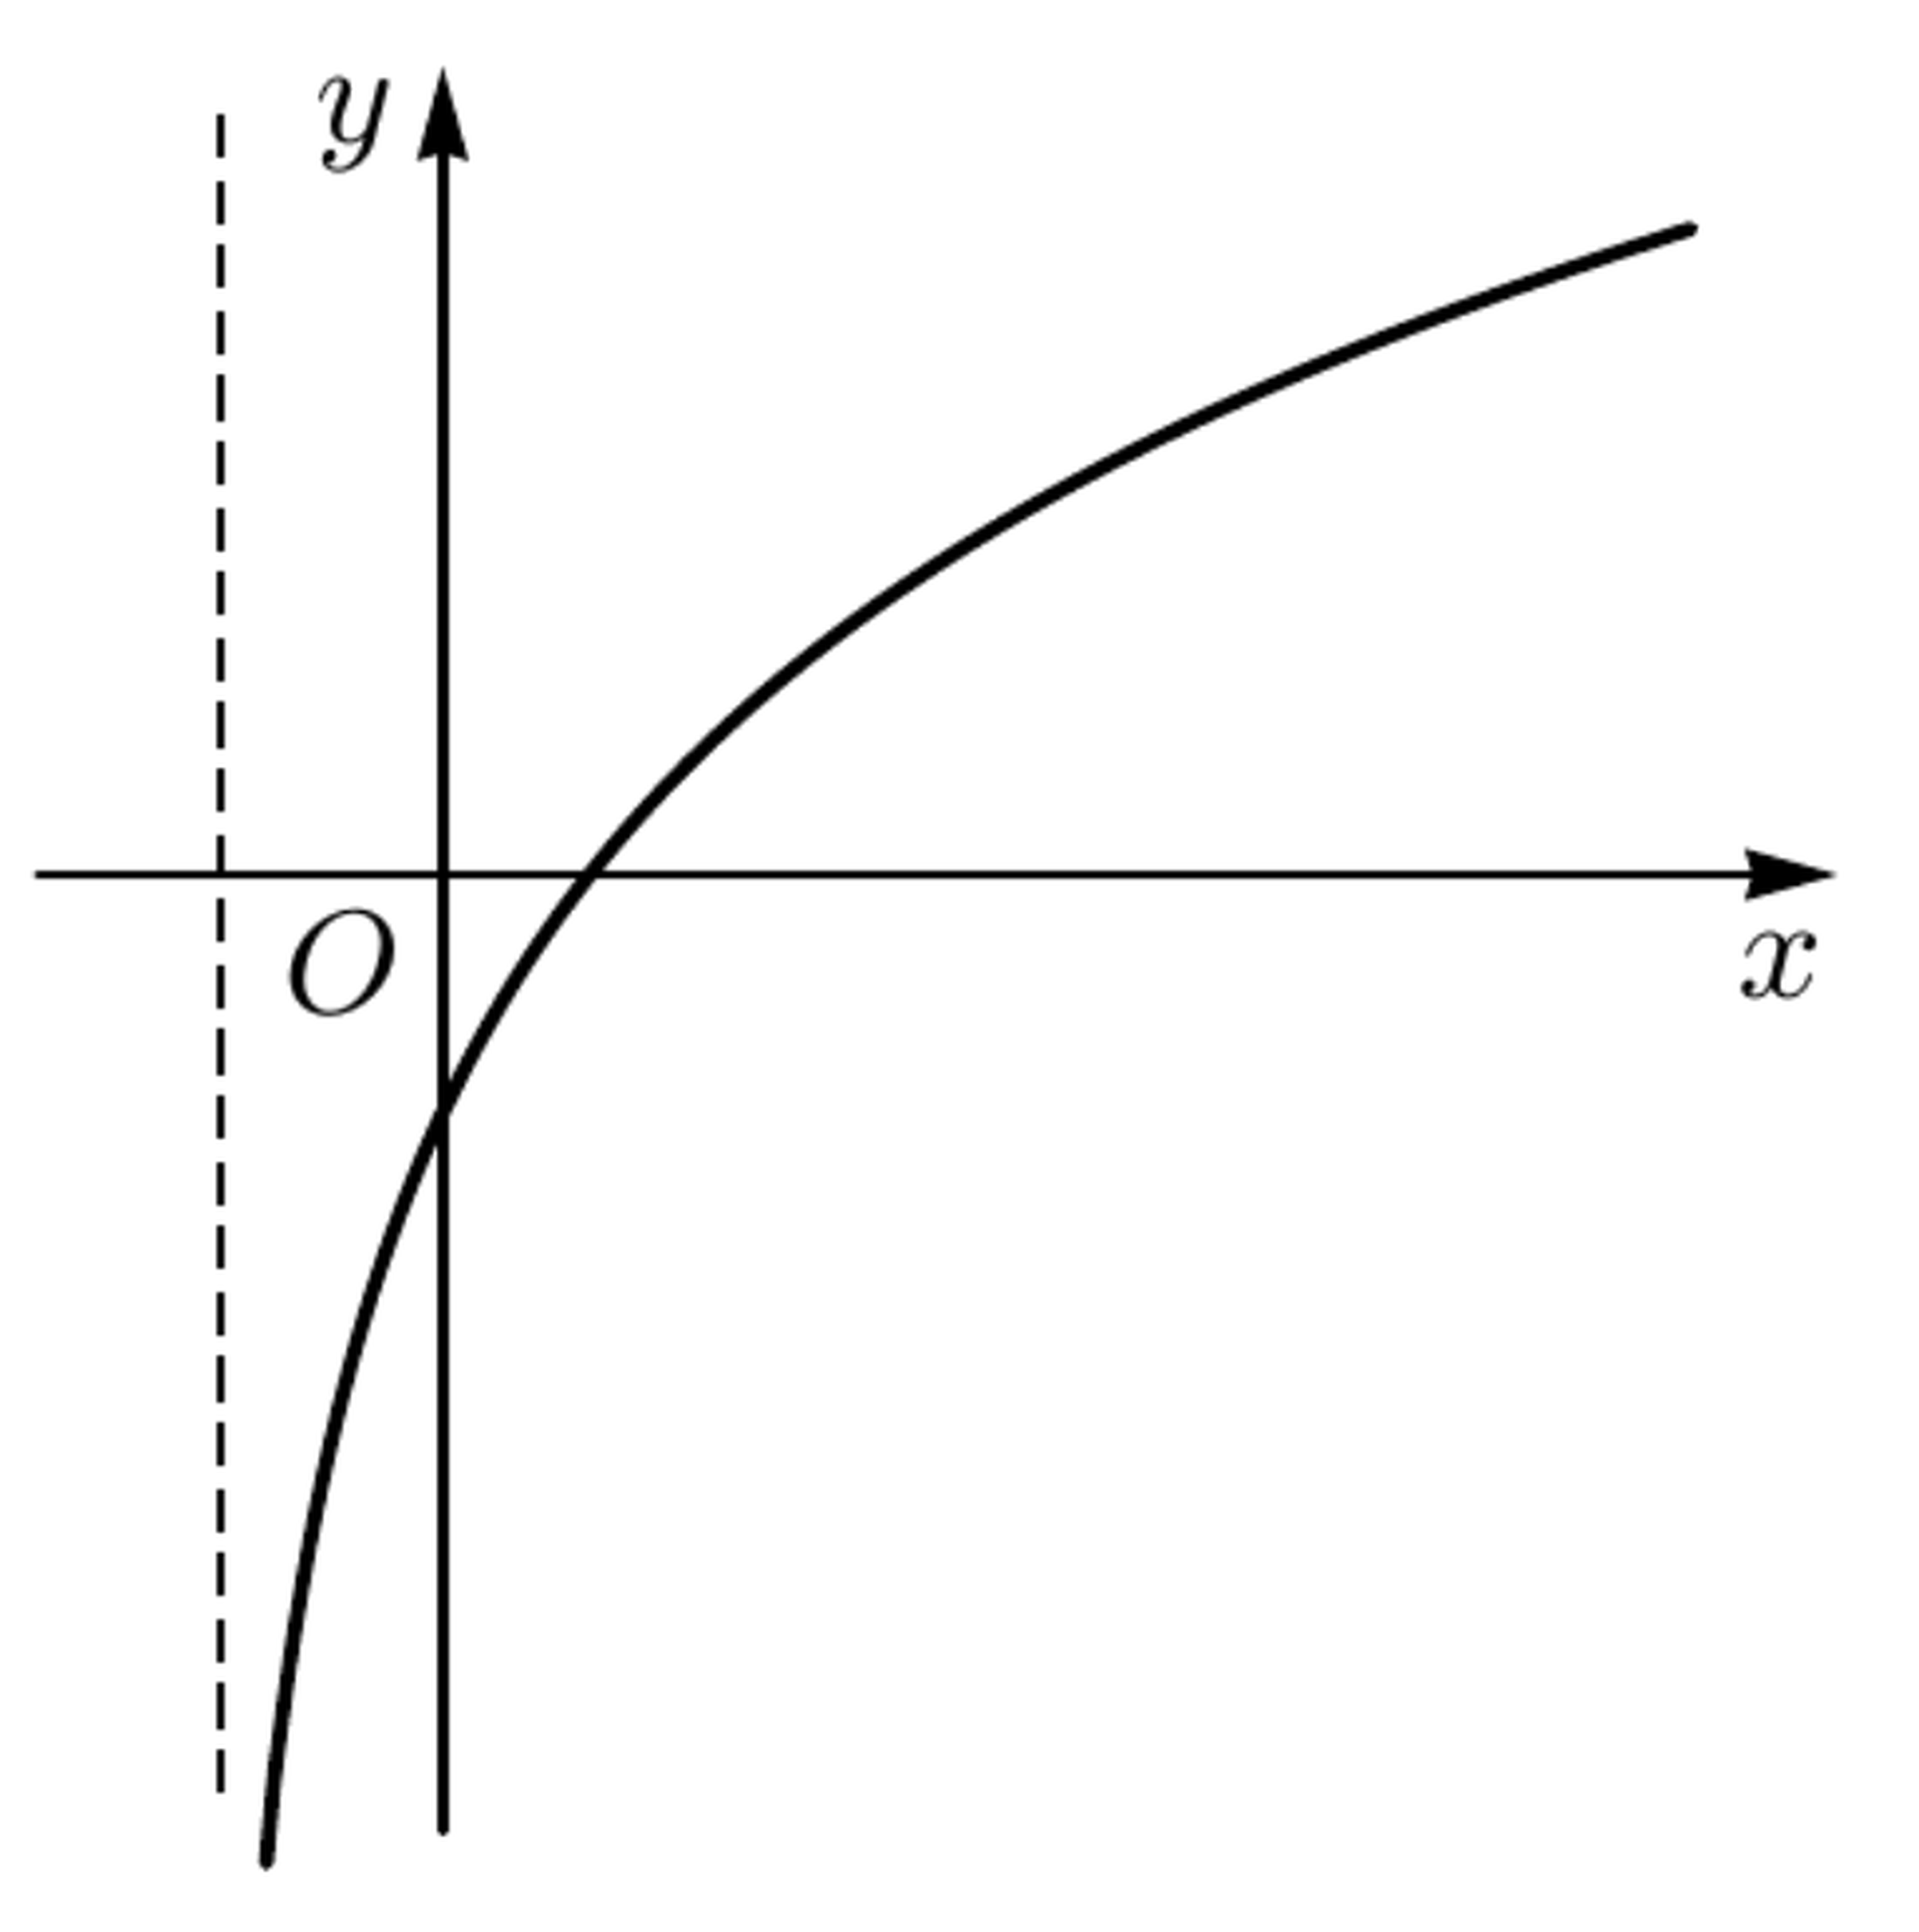
\includegraphics[width=0.42\textwidth]{figures/gao158_q15.png}
\end{center}

\keepwithprev
A. $a>1, b>1$\qquad\qquad B. $a>1, 0<b<1$

C. $0<a<1, b>1$\qquad\qquad D. $0<a<1, 0<b<1$

\ifanswer
\solbegin
\step{图像严格增，得 $a>1$.}
\step{图像与 $y$ 轴交于 $x$ 轴下方，得 $b>0$ 且 $\log_a b<0$，即 $0<b<1$，故选 $B$.}
\solend
\fi

% === Q16 === \lvert\log_2 x\rvert；解析 5 行，故选 C
\item 已知函数 $f(x)=\lvert\log_2 x\rvert$，若 $0<a<b$ 且 $f(a)=f(b)$，则 $a+2b$ 的取值范围是\mbox{（\quad）}

\keepwithprev
A. $(2\sqrt2,+\infty)$\qquad B. $[2\sqrt2,+\infty)$\qquad C. $(3,+\infty)$\qquad D. $[3,+\infty)$

\ifanswer
\solbegin
\step{由 $a<b$ 及 $\lvert\log_2 a\rvert=\lvert\log_2 b\rvert$，得 $\log_2 a=-\log_2 b$，即 $ab=1$，}
\step{且 $0<a<1<b$.}
\step{设 $t=a+2b=2b+\dfrac1b$，则 $t-3=\dfrac{(b-1)(2b-1)}{b}>0$.}
\step{反之，任取 $t>3$，令 $b=\dfrac{t+\sqrt{t^2-8}}{4}>1$、$a=\dfrac1b$，则满足题设且 $a+2b=t$.}
\step{因此取值范围为 $(3,+\infty)$，故选 $C$.}
\solend
\fi

\end{enumerate}

\bigsec{三、解答题}

\begin{enumerate}
\setcounter{enumi}{16}

% === Q17 === 集合、\overline{A}、\subseteq；解析 9 行
\item 已知全集 $U=\R$，集合 $A=\left\{x\mid\dfrac{x-3}{x+1}\leqslant0\right\}$，$B=\{x\mid x^2-2mx+m^2-9<0\}$（$m$ 为实数）.

(1) 当 $m=4$ 时，求 $A\cap B$ 和 $\overline{A}\cup B$；

(2) 若“$x\in A$”是“$x\in B$”的充分条件，求实数 $m$ 的取值范围.

\ifanswer
\solbegin
\step{(1) $\dfrac{x-3}{x+1}\leqslant0\Leftrightarrow-1<x\leqslant3$，所以 $A=(-1,3]$.}
\step{当 $m=4$ 时，$B=\{x\mid(x-4)^2<9\}=(1,7)$，}
\step{于是 $A\cap B=(1,3]$，$\overline{A}\cup B=(-\infty,-1]\cup(1,+\infty)$；}
\step{(2) $x^2-2mx+m^2-9<0\Leftrightarrow(x-m)^2<9$，所以 $B=(m-3,m+3)$.}
\step{题设充分条件等价于 $A\subseteq B$.}
\step{由于 $A=(-1,3]$，左端须满足 $m-3\leqslant-1$.}
\step{又 $3\in A$，须有 $3<m+3$.}
\step{这两个条件也保证 $(-1,3]\subseteq(m-3,m+3)$，}
\step{因此 $A\subseteq B\Leftrightarrow\begin{cases}m-3\leqslant-1\\m+3>3\end{cases}\Leftrightarrow0<m\leqslant2$.}
\solend
\fi

% === Q18 === 蓄水池造价（含 (3) 场地限制）；单位 \mathrm{m}；解析 13 行
\item 某工厂拟建一个容积为 $400\mathrm{m}^3$ 的无盖长方体蓄水池，池深 $4\mathrm{m}$，池底为矩形，其一边长
为 $x\mathrm{m}$. 池壁每平方米造价 100 元，池底每平方米造价 150 元. 设水池的总造价为 $C$
元.

(1) 把 $C$ 表示成 $x$ 的函数，并写出它的定义域；

(2) 当 $x$ 为何值时，总造价最低？最低造价是多少？

(3) 受场地限制，池底一边长 $x$ 不超过 $8\mathrm{m}$，此时总造价最低是多少？

\ifanswer
\solbegin
\step{(1) 设池底另一边长为 $y\mathrm{m}$，则 $4xy=400$，所以 $y=\dfrac{100}{x}$，$x>0$.}
\step{池底面积为 $100\mathrm{m}^2$，池壁总面积为 $8\left(x+\dfrac{100}{x}\right)\mathrm{m}^2$，}
\step{因此 $C(x)=100\times8\left(x+\dfrac{100}{x}\right)+150\times100=800x+\dfrac{80000}{x}+15000$，}
\step{定义域为 $(0,+\infty)$.}
\step{(2) 因为 $x>0$，所以 $C(x)=800\left(x+\dfrac{100}{x}\right)+15000$，}
\step{$\geqslant800\times2\sqrt{x\cdot\dfrac{100}{x}}+15000=31000$，}
\step{当且仅当 $x=\dfrac{100}{x}$，即 $x=10$ 时取等号.}
\step{答：当 $x=10$ 时，总造价最低，为 31000 元.}
\step{(3) 此时定义域为 $(0,8]$. 任取 $0<x_1<x_2\leqslant8$，}
\step{则 $C(x_2)-C(x_1)=800(x_2-x_1)\left(1-\dfrac{100}{x_1x_2}\right)<0$，}
\step{所以 $C(x)$ 在 $(0,8]$ 上严格递减，$x=8$ 时总造价最低，}
\step{且 $C(8)=800\times8+\dfrac{80000}{8}+15000=31400$.}
\step{答：受场地限制时，最低总造价为 31400 元.}
\solend
\fi

% === Q19 === 甲乙滤材 0.8^n／0.7^n；解析 17 行
\item 某环保公司研发了两种新型滤材甲和乙：污水每经过一层甲滤材，污染物含量减少
20\%；每经过一层乙滤材，污染物含量减少 30\%. 每层甲滤材成本 3 万元，每层乙滤材
成本 4 万元. 设原污水中污染物含量为 1，要求处理后污染物含量低于原来的 5\%.

(1) 若只使用一种滤材，污水经过 $n$ 层后污染物含量为 $y$，分别写出使用甲、乙两种滤材
时 $y$ 关于 $n$ 的函数关系式（$n$ 为正整数）；

(2) 若只使用一种滤材，分别求甲、乙至少各需要多少层，并比较哪种滤材的总成本更
低；

(3) 若两种滤材可以混合使用（先后顺序不影响效果），设使用甲滤材 $m$ 层、乙滤材 $n$
层（$m$、$n$ 为非负整数），求满足要求的最低总成本，并指出此时 $m$、$n$ 的值.

\ifanswer
\solbegin
\step{(1) 甲：$y=0.8^n$；乙：$y=0.7^n$，其中 $n$ 为正整数.}
\step{(2) 两种滤材均须满足 $y<0.05$，且污染物含量随层数增加而严格减少.}
\step{$0.8^{14}\approx0.04398<0.05<0.05498\approx0.8^{13}$，}
\step{$0.7^9=0.040353607<0.05<0.05764801=0.7^8$，}
\step{甲至少需要 14 层，成本为 $3\times14=42$ 万元；}
\step{乙至少需要 9 层，成本为 $4\times9=36$ 万元.}
\step{因此，只使用一种滤材时，使用乙滤材的总成本更低.}
\step{(3) 设总成本为 $C$ 万元，则 $C=3m+4n,0.8^m\cdot0.7^n<0.05,m,n\in\{0,1,2,\cdots\}$，}
\step{若 $m\geqslant3$，将其中 3 层甲替换为 2 层乙，}
\step{因为 $0.7^2=0.49<0.512=0.8^3,2\times4<3\times3$，}
\step{替换后污染物含量更低，成本减少 1 万元，因此最低成本方案必有 $m\leqslant2$.}
\step{当 $m=0$ 时，由第（2）小题得至少需要 9 层乙，最低成本为 36 万元.}
\step{当 $m=1$ 或 $m=2$ 时，$0.8\cdot0.7^7>0.8^2\cdot0.7^7=0.052706752>0.05$，}
\step{$0.8^2\cdot0.7^8<0.8\cdot0.7^8=0.046118408<0.05$，}
\step{因此两种情形均至少需要 8 层乙，}
\step{对应最低成本分别为 $3+4\times8=35$ 万元，$3\times2+4\times8=38$ 万元.}
\step{答：满足要求的最低总成本为 35 万元，此时使用甲滤材 1 层、乙滤材 8 层.}
\solend
\fi

% === Q20 === f(x)=\log_2(4^x+1)-x；\Delta；解析 17 行
\item 已知函数 $f(x)=\log_2(4^x+1)-x$.

(1) 证明 $f(x)=\log_2(2^x+2^{-x})$，并求 $f(x)$ 的最小值及取得最小值时 $x$ 的值；

(2) 解不等式 $f(x)>\log_2 5-1$；

(3) 证明：函数 $f(x)$ 在区间 $[0,+\infty)$ 上是严格增函数；并求使关于 $x$ 的方程 $f(x)=m$ 恰
有两个不同实数解的实数 $m$ 的取值范围.

\ifanswer
\solbegin
\step{(1) $f(x)=\log_2(4^x+1)-\log_2 2^x=\log_2\dfrac{4^x+1}{2^x}=\log_2(2^x+2^{-x})$，}
\step{因为 $2^x+2^{-x}\geqslant2\sqrt{2^x\cdot2^{-x}}=2$，所以 $f(x)\geqslant\log_2 2=1$，}
\step{等号当且仅当 $2^x=2^{-x}$，即 $x=0$ 时成立，故最小值为 1.}
\step{(2) 令 $t=2^x>0$，则 $f(x)>\log_2 5-1\Leftrightarrow t+\dfrac1t>\dfrac52\Leftrightarrow2t^2-5t+2>0$}
\step{$\Leftrightarrow(2t-1)(t-2)>0$，}
\step{结合 $t>0$，得 $0<t<\dfrac12$ 或 $t>2$，即 $x<-1$ 或 $x>1$，}
\step{解集为 $(-\infty,-1)\cup(1,+\infty)$.}
\step{(3) 任取 $0\leqslant x_1<x_2$，记 $a=2^{x_1}$，$b=2^{x_2}$，则 $1\leqslant a<b$，$ab>1$，}
\step{从而 $\left(b+\dfrac1b\right)-\left(a+\dfrac1a\right)=(b-a)\left(1-\dfrac{1}{ab}\right)>0$，}
\step{由对数函数的严格递增性，得 $f(x_1)<f(x_2)$，}
\step{所以 $f(x)$ 在 $[0,+\infty)$ 上是严格增函数.}
\step{当 $m<1$ 时，由（1）得方程无实数解；当 $m=1$ 时，只有实数解 $x=0$.}
\step{当 $m>1$ 时，令 $t=2^x>0$，则 $f(x)=m\Leftrightarrow t+\dfrac1t=2^m\Leftrightarrow t^2-2^m t+1=0$，}
\step{此时 $\Delta=2^{2m}-4>0$，两根之和为 $2^m>0$、之积为 $1>0$，}
\step{故有两个不同的正根.}
\step{每个正根 $t$ 唯一确定一个实数 $x=\log_2 t$，故原方程恰有两个不同实数解，}
\step{所求范围为 $m\in(1,+\infty)$.}
\solend
\fi

% === Q21 === f(x)=4^x-m\cdot2^{x+1}+3 值域与 h(m) 分段；解析 13 行
\item 已知函数 $f(x)=4^x-m\cdot2^{x+1}+3$（$m\in\R$），$x\in[0,2]$.

(1) 当 $m=1$ 时，求 $f(x)$ 的值域；

(2) 记 $f(x)$ 的最小值为 $h(m)$，求 $h(m)$ 的表达式；

(3) 若关于 $x$ 的方程 $f(x)=0$ 在区间 $[0,2]$ 上有解，求实数 $m$ 的取值范围.

\ifanswer
\solbegin
\step{令 $t=2^x$，则 $t\in[1,4]$，且 $f(x)=t^2-2mt+3=(t-m)^2+3-m^2$，}
\step{(1) 当 $m=1$ 时，$f(x)=(t-1)^2+2$.}
\step{由 $0\leqslant t-1\leqslant3$，得 $2\leqslant f(x)\leqslant11$，值域为 $[2,11]$.}
\step{(2) 二次函数 $y=(t-m)^2+3-m^2$ 的对称轴为直线 $t=m$.}
\step{当 $m\leqslant1$ 时，在 $t=1$ 处取最小值；}
\step{当 $1<m<4$ 时，在 $t=m$ 处取最小值；}
\step{当 $m\geqslant4$ 时，在 $t=4$ 处取最小值；}
\step{因此 $h(m)=\begin{cases}4-2m,&m\leqslant1\\3-m^2,&1<m<4\\19-8m,&m\geqslant4\end{cases}$；}
\step{(3) 方程 $f(x)=0$ 在 $[0,2]$ 上有解，}
\step{等价于存在 $t\in[1,4]$，使 $m=\dfrac{t^2+3}{2t}=\dfrac12\left(t+\dfrac3t\right)$，}
\step{由基本不等式，$m\geqslant\dfrac12\cdot2\sqrt{t\cdot\dfrac3t}=\sqrt3$，当且仅当 $t=\sqrt3$ 时取等号；}
\step{又 $\dfrac{19}{8}-m=\dfrac{(4-t)(4t-3)}{8t}\geqslant0$，当且仅当 $t=4$ 时取等号；}
\step{因此必有 $\sqrt3\leqslant m\leqslant\dfrac{19}{8}$.}
\solend
\fi

\end{enumerate}

\end{document}
"
%
% ① 原始材料：微信公众号"魔都数学加油站"文章，连载"27学年高一158"，原文标题
% "27学年高一158——2026-2027年上海市上实东滩高一上期中"（本卷本地编号 158 与
% 原卷连载号一致，无撞号）。
% 正文为 9 张 PNG 页（01/05/08/09 为 2560×3620，02/03/04/06/07 为 4762×6735，
% 同一篇各页分辨率混排，逐页按各自分辨率裁图核对）。
% 体例：讲评版——填空 3—12（10 题）、选择 13—16（4 题）、解答 17—21（5 题），
% 共 19 题，自第 3 题起编（1、2 未印在本篇）；Q5 只印【答案】、其余 18 题
% 逐题印【解析】（逐题核实，见 ②）。题目、答案、解析均据原图转录；卷面粉红色
% 水印"魔都数学加油站"及公众号页脚未录入。全卷末题为第 21 题，无附加题节。
% 全卷 2 组配图（逐页通读 9 页确认）——
%   · Q10 题干右侧"曼 → man"字形变换图（02 页），题目配图、三版都出，
%     裁 figures/gao158_q10.png；
%   · Q15 题干"如图所示"对数函数大致图像（03 页右下），题目配图、三版都出，
%     裁 figures/gao158_q15.png；
% 2 图均取自原卷截图，去粉色水印、转灰度、4× LANCZOS 放大；
% 其余各页逐页确认无其它题目配图、无解析内配图、无表格。
%
% 卷首标题：原卷印作"2026-2027 年上实东滩高一上期中"，年份区间按全稿惯例排 en dash；
% 原卷卷面未印副标题，本稿按同期中卷知识模块口径补出"集合与常用逻辑用语、不等式、函数"。
%
% ② 与原卷的排版差异／照录项清单：
%   ① 原文从第 3 题起，本稿保留原题号；共 19 题三节，解答题 5 题到 21；
%      三节各自一个 enumerate＋各自 \setcounter{enumi}{2}／{12}／{16}，
%      不贯穿（题目溯源.py 按 \bigsec 切节、每节独立计 depth，只收 depth==1 的 \item）；
%   ② 混合体例：Q5 只印【答案】、无【解析】，按 高一156 第 3 题成例另提
%      \ans{}、不补造解析；其余 18 题印【解析】、用 \solbegin…\solend；
%      四道选择题答案均在解析末句"故选 C／B／B／C"（逐个放大复核）、
%      题干括号 \mbox{（\quad）} 留空、不另提 \ans{}；答案版
%      【答案】/【解析】标记数 = 19 = 全卷题数（1 个 \ans ＋ 18 个 \solbegin）；
%   ③ 原卷卷面未印副标题，本稿按知识模块口径补出；
%   ④ 原卷填空横线按全稿惯例排 \blankline[4.4em]；选择题选项段前按惯例各加
%      \keepwithprev；解答题不留作答区、不加 \anspace（原卷为讲评版）；
%   ⑤ 数集：Q13"在 \R 上严格递增"、Q14"$x\in\R$"、Q17"$U=\R$"、
%      Q21"$m\in\R$" 原卷印正体粗体 R，按全稿惯例归一 \R；
%      绝对值排 \lvert…\rvert（Q12 $\lvert a\rvert$、Q14 $\lvert x-2\rvert$、
%      Q16 $\lvert\log_2 x\rvert$／$\lvert\log_2 a\rvert$／$\lvert\log_2 b\rvert$），
%      集合描述竖线排 \mid（Q17），不等号按全稿惯例排 \leqslant／\geqslant，
%      补集上划线 \overline{A}（Q17）；
%   ⑥ 子集／真子集符号逐处照录不统一：Q14 解析"$(2,3)\subsetneq(1,3)$"原卷印
%      带下划线且被斜杠划过的 ⊊（真子集，放大 03 页确认），照录 \subsetneq；
%      Q17 解析三处"$A\subseteq B$""$(-1,3]\subseteq(m-3,m+3)$"原卷印
%      带下划线 ⊆（放大 05 页确认），照录 \subseteq；本卷无单线 \subset 用例；
%   ⑦ 判别式：Q20 (3) 解析"$\Delta=2^{2m}-4>0$"原卷印高瘦等腰 \Delta
%      （像素实测高/宽 ≈ 1.13，扁三角 \triangle 为 0.93，放大 08 页确认），
%      照录 \Delta；本卷无扁三角 \triangle 用例；
%   ⑧ "图像"与"图象"：全卷统一用"图像"（Q6 题干、Q10 两处、Q11 解析、
%      Q15 题干与解析两处，逐处放大确认带单人旁），照录不改；
%   ⑨ 中文弯引号照录：Q5 命题"若实数…"、Q10"曼""man""新"、Q14 题干与
%      解析的两则不等式、Q17 (2)"$x\in A$""$x\in B$"；注释里一律 ASCII 引号；
%   ⑩ 半角逗号逐处照录：Q8"$2,3,4$""$-2,-1,0$"、Q10 点坐标 $(x,y)$／
%      $(t,2^t-1)$／$(1-2^t,t)$、Q15 四选项"$a>1, b>1$"等、
%      Q19 (3)"$C=3m+4n,0.8^m\cdot0.7^n<0.05,m,n\in\{0,1,2,\cdots\}$"
%      与"$0.7^2=0.49<0.512=0.8^3,2\times4<3\times3$"、
%      Q21 cases 内"$4-2m,$"等；其余行中逗号／顿号照录全角；
%      行末西文句点 ASCII `.`；
%   ⑪ 顿号照录：Q3"（用 $a$、$b$ 表示）"、Q5"$x$、$y$"、Q13"A、B"、
%      Q16 解析"$>1$、$a=\dfrac1b$"、Q19"甲、乙""$m$、$n$"、
%      Q20"$2^m>0$、之积为"、Q21"$m$、$n$"；顿号一律移到数学模式外，
%      数学模式内不出现中文标点；
%   ⑫ 角度与单位照录：Q10 三处"$90^{\circ}$"、Q18"$400\mathrm{m}^3$"
%      "$4\mathrm{m}$""$x\mathrm{m}$""$8\mathrm{m}$""$y\mathrm{m}$"
%      "$100\mathrm{m}^2$""$\left(x+\dfrac{100}{x}\right)\mathrm{m}^2$"；
%      Q19 百分号"20\%""30\%""5\%"按原卷排 \%；
%   ⑬ 文本模式全角括号照录：Q10"（提示：…）"、Q17"（$m$ 为实数）"、
%      Q19"（$n$ 为正整数）""（先后顺序不影响效果）""（$m$、$n$ 为非负整数）"、
%      Q20"由（1）得"、Q19"由第（2）小题"、Q21"（$m\in\R$）"；
%      子题行首标号按全稿惯例用半角 (1)(2)(3)；
%   ⑭ 复杂式照录别简化：Q3 $\dfrac{\log_3 2+\log_3 5}{\log_3 3+2\log_3 2}$、
%      Q8 $[-3,-2)\cup(4,5]$、Q9 $18ab=2^t\cdot3^t=6^t=a+b$、
%      Q12 $\dfrac{\sqrt6}{2}$、Q18 $C(8)=800\times8+\dfrac{80000}{8}+15000=31400$
%      （原卷即 C(8)，非 C(2)）、Q19 $0.8^{14}\approx0.04398$、
%      $0.7^9=0.040353607$、$0.052706752$、$0.046118408$、
%      Q20 $t^2-2^m t+1=0$、Q21 $h(m)$ 三段 cases 与 $\dfrac{(4-t)(4t-3)}{8t}$ 等；
%      \left…\right 不得拆到不同 $…$ 组；cases 块整体算一个印刷行；
%   ⑮ 一条 \step = 原卷解析的一个印刷行；别并折行、别拆行。跨页续印按题合并
%      （Q7 的 01—02 页、Q9/Q10/Q11 的 02—03 页、Q13/Q14 的 03 页上下、
%      Q15/Q16 的 04 页上下、Q17 的 04—05 页、Q18 的 05—06 页、
%      Q19 的 06—07 页、Q20 的 07—08 页、Q21 的 08—09 页）；
%      跨半页重叠行（Q5【答案】、Q9 设公共值行、Q10 题干、Q16 反之行、
%      Q18 (2) 题干、Q19 末两行、Q20 (3) 末行、Q21 cases 块）只算一个印刷行；
%   ⑯ 配图：2 组题目配图（见 ①），均三版都出，\needvspace 守卫放 \item 之前
%      把"题干＋图"整块推走，\includegraphics 放题干之后；本卷无解析内配图、
%      无红字加粗小标题（全卷逐页确认，故无 \stepm）。
%
% ③ 行数复核：一条 \step = 原卷解析的一个印刷行，cases 块作一个印刷行计。
%   逐题数（逐页核对）：Q3：1；Q4：2；Q5：0（只印【答案】、提 \ans{}，
%   不计入 \step 账）；Q6：1；Q7：4；Q8：5；Q9：2；Q10：2；Q11：3；
%   Q12：3；Q13：2；Q14：3；Q15：2；Q16：5；Q17：9；Q18：13；
%   Q19：17；Q20：17；Q21：13。
%   合计 104 行（104 条 \step ＋ 0 条 \stepm），与原卷逐题印刷行相等。
%   全卷 19 题：Q5 一处 \ans{} ＋ 其余 18 题设 \solbegin…\solend，
%   答案版【答案】/【解析】标记数 = 19 = 全卷题数。
%
% ④ 页码分布（供回原图复核）：
%   卷首标题＋"一、填空题"＋Q3 题干＋解析 1 行、Q4 题干＋解析 2 行、
%   Q5 题干＋【答案】在 01 页上半；Q5【答案】（重叠重印）＋Q6 题干＋解析 1 行、
%   Q7 题干＋解析前 3 行在 01 页下半；Q7 解析末行＋Q8 题干＋解析 5 行、
%   Q9 题干＋解析首行在 02 页上半；Q9 解析末行＋Q10 题干（含"曼→man"图）
%   ＋解析 2 行＋Q11 题干＋解析首行在 02 页下半；Q11 解析后 2 行＋Q12 题干
%   ＋解析 3 行＋"二、选择题"标题＋Q13 题干＋选项在 03 页上半；
%   Q13 选项（重叠重印）＋解析 2 行＋Q14 题干＋选项＋解析 3 行＋Q15 题干
%   ＋对数图像（右侧）在 03 页下半；Q15 选项＋解析 2 行＋Q16 题干＋选项
%   ＋解析前 4 行在 04 页上半；Q16 解析末行＋"三、解答题"标题＋Q17 题干
%   ＋两问＋解析 (1) 3 行在 04 页下半；Q17 解析 (2) 6 行＋Q18 题干＋三问
%   ＋解析 (1) 4 行＋(2) 首行在 05 页上下；Q18 解析 (2) 后 3 行＋(3) 5 行
%   ＋Q19 题干＋三问＋解析 (1) 1 行＋(2) 3 行在 06 页上下；Q19 解析 (2) 3 行
%   ＋(3) 12 行在 07 页上半；Q19 解析末 2 行（重叠）＋Q20 题干＋三问
%   ＋解析 (1) 3 行在 07 页下半；Q20 解析 (2) 4 行＋(3) 前 4 行在 08 页上半；
%   Q20 解析 (3) 后 6 行＋Q21 题干＋(1) 问在 08 页下半；Q21 (2)(3) 问＋
%   解析 (1) 3 行＋(2) 5 行＋cases 块在 09 页上半；Q21 cases 块（重叠）
%   ＋(3) 解析 5 行在 09 页下半。本稿按题连排，不丢行、不并折行；
%   全卷末题为第 21 题，无附加题节。
%
% ⑤ 存疑／需主会话回原图复核：
%   1. Q14 解析"$(2,3)\subsetneq(1,3)$"的 ⊊（真子集带斜杠）与 Q17 的 ⊆
%      是两种不同记号，本稿分别照录 \subsetneq／\subseteq，请复核；
%   2. Q20 (3)"$\Delta=2^{2m}-4>0$"判为高瘦 \Delta，请复核是否 \triangle；
%   3. 任务书提示"Q18 解析里印 C(2)=…"，但 06 页原图逐处读作
%      $C(8)=800\times8+\dfrac{80000}{8}+15000=31400$，未找到 C(2)，
%      本稿照原卷排 C(8)，请复核；
%   4. Q19 解析末句"最低总成本为 35 万元"（07 页上下两处印同），
%      OCR 曾误读为 34，本稿按 35 照录，请复核；
%   5. Q10 提示末尾"坐标为 $(-y,x)$）."为半角 $)$＋全角 $）$ 两枚括号，
%      本稿照录，请复核；
%   6. Q21 cases 块后"；"落在分式中行右侧（排版居中基线所致），
%      本稿排作 $…\end{cases}$；，请复核。
%   全卷除此 6 类外未发现其它笔误／自相矛盾处；19 题中 18 题印【解析】。
%
\documentclass[a4paper,11pt]{article}
\usepackage{common}

\begin{document}

\examtitlest[3]{2026--2027 年上实东滩高一上期中}{集合与常用逻辑用语、不等式、函数}

\bigsec{一、填空题}

\begin{enumerate}
\setcounter{enumi}{2}

% === Q3 === 换底公式；解析 1 行
\item 已知 $3^a=5$，$\log_3 2=b$，则 $\log_{12} 10=$\blankline[4.4em]（用 $a$、$b$ 表示）.

\ifanswer
\solbegin
\step{$\log_{12} 10=\dfrac{\log_3 2+\log_3 5}{\log_3 3+2\log_3 2}=\dfrac{a+b}{1+2b}$.}
\solend
\fi

% === Q4 === 定义域；解析 2 行；半角括号 ( ) 与全角逗号照录
\item 函数 $y=\sqrt{2-x}+\lg(x^2-1)$ 的定义域为\blankline[4.4em].

\ifanswer
\solbegin
\step{由 $2-x\geqslant0$ 且 $x^2-1>0$，得 $x\leqslant2$ 且 ($x<-1$或$x>1$)，}
\step{定义域为 $(-\infty,-1)\cup(1,2]$.}
\solend
\fi

% === Q5 === 只印【答案】、无【解析】；反证法，中文弯引号
\item 用反证法证明命题“若实数 $x$、$y$ 满足 $x+y>2$，则 $x$、$y$ 中至少有一个大于 1”时，
应假设\blankline[4.4em].

\ifanswer
\ans{$x\leqslant1$ 且 $y\leqslant1$}
\fi

% === Q6 === 图像平移；解析 1 行
\item 函数 $y=\dfrac{2x+1}{x-1}$ 的图像可由函数 $y=\dfrac{3}{x}$ 的图像先向右平移 $a$ 个单位，再向上平移 $b$ 个单位
得到，则 $a+b=$\blankline[4.4em].

\ifanswer
\solbegin
\step{$y=\dfrac{2x+1}{x-1}=\dfrac{3}{x-1}+2$，所以 $a=1$，$b=2$，$a+b=3$.}
\solend
\fi

% === Q7 === 集合三元子集；解析 4 行，跨 01—02 页
\item 设 $A=\{a_1,a_2,a_3,a_4\}$ 是由四个实数组成的集合，若 $A$ 的所有三元子集中，三个元素之和
组成的集合为 $B=\{1,4,7,12\}$，则集合 $A=$\blankline[4.4em].

\ifanswer
\solbegin
\step{设 $S=a_1+a_2+a_3+a_4$，}
\step{每个元素在四个三元子集中恰出现三次，则 $3S=1+4+7+12=24$，得 $S=8$.}
\step{四个三元子集的元素和分别为 $S-a_i$，}
\step{所以 $A=\{8-1,8-4,8-7,8-12\}=\{-4,1,4,7\}$.}
\solend
\fi

% === Q8 === 不等式整数解；解析 5 行；半角逗号照录
\item 不等式 $x^2-(a+1)x+a<0$ 的解集中恰有 3 个整数，则 $a$ 的取值范围是\blankline[4.4em].

\ifanswer
\solbegin
\step{原不等式为 $(x-1)(x-a)<0$；}
\step{$a=1$ 时解集为空集，不符合题意.}
\step{若 $a>1$，解集为 $(1,a)$，恰含整数 $2,3,4$，则 $4<a\leqslant5$.}
\step{若 $a<1$，解集为 $(a,1)$，恰含整数 $-2,-1,0$，则 $-3\leqslant a<-2$.}
\step{故 $a$ 的取值范围是 $[-3,-2)\cup(4,5]$.}
\solend
\fi

% === Q9 === 对数换底＋指数；解析 2 行
\item 已知正数 $a$、$b$ 满足 $1+\log_2 a=2+\log_3 b=\log_6(a+b)$，则 $\dfrac1a+\dfrac1b=$\blankline[4.4em].

\ifanswer
\solbegin
\step{设公共值为 $t$，则 $2a=2^t$，$9b=3^t$，$a+b=6^t$，}
\step{于是 $18ab=2^t\cdot3^t=6^t=a+b$，即 $\dfrac1a+\dfrac1b=\dfrac{a+b}{ab}=18$.}
\solend
\fi

% === Q10 === "曼"字旋转 90°；题目配图（三版都出）；解析 2 行
\needvspace{6cm}
\item 网上流传一个有趣的字形变换：把汉字“曼”的右半部分旋转 $90^{\circ}$，就得到英文单词
“man”的艺术字. 数学中，把曲线绕原点旋转也会得到“新”的曲线：将函数
$y=2^x-1$ 的图像绕坐标原点 $O$ 逆时针旋转 $90^{\circ}$，得到的曲线恰是某个函数的
图像，则这个函数的解析式为\blankline[4.4em]（提示：点 $(x,y)$ 绕 $O$ 逆时针旋转 $90^{\circ}$ 后的
坐标为 $(-y,x)$）.

\begin{center}

\includegraphics[width=0.42\textwidth]{figures/gao158_q10.png}
\end{center}

\ifanswer
\solbegin
\step{原图像上的点 $(t,2^t-1)$ 旋转后为 $(1-2^t,t)$.}
\step{记其为 $(x,y)$，则 $x=1-2^y$，即 $y=\log_2(1-x)$，定义域为 $(-\infty,1)$.}
\solend
\fi

% === Q11 === 值域；解析 3 行，跨 02—03 页
\item 函数 $f(x)=\sqrt{x-2}-\sqrt{15-3x}$ 的值域为\blankline[4.4em].

\ifanswer
\solbegin
\step{由 $x-2\geqslant0$ 且 $15-3x\geqslant0$，得定义域为 $[2,5]$.}
\step{在 $[2,5]$ 上，$\sqrt{x-2}$ 与 $-\sqrt{15-3x}$ 均严格递增，因此 $f(x)$ 严格递增.}
\step{$f(2)=-3$，$f(5)=\sqrt3$，结合函数的图像，值域为 $[-3,\sqrt3]$.}
\solend
\fi

% === Q12 === 绝对值 \lvert…\rvert；解析 3 行
\item 设实数 $a$ 满足 $a<4a^3-5a<\lvert a\rvert$，则 $a$ 的取值范围是\blankline[4.4em].

\ifanswer
\solbegin
\step{由 $a<\lvert a\rvert$ 得 $a<0$，原不等式为 $a<4a^3-5a<-a$.}
\step{同除以 $a<0$，得 $1>4a^2-5>-1\Leftrightarrow1<a^2<\dfrac32$，结合 $a<0$，}
\step{得 $-\dfrac{\sqrt6}{2}<a<-1$，故解集为 $\left(-\dfrac{\sqrt6}{2},-1\right)$.}
\solend
\fi

\end{enumerate}

\bigsec{二、选择题}

\begin{enumerate}
\setcounter{enumi}{12}

% === Q13 === \R 归一；解析 2 行，故选 C
\item 已知 $a>b$，则下列不等式一定成立的是\mbox{（\quad）}

\keepwithprev
A. $\dfrac1a<\dfrac1b$\qquad B. $a^2>b^2$\qquad C. $a^3>b^3$\qquad D. $ac^2>bc^2$

\ifanswer
\solbegin
\step{幂函数 $y=x^3$ 在 $\R$ 上严格递增，$a>b\Rightarrow a^3>b^3$，C 正确.}
\step{取 $a=1$，$b=-1$ 得 A、B 不成立；取 $c=0$ 得 D 不成立；故选 $C$.}
\solend
\fi

% === Q14 === \subsetneq 真子集；解析 3 行，故选 B
\item 设 $x\in\R$，则“$\lvert x-2\rvert<1$”是“$x^2-5x+6<0$”的\mbox{（\quad）}

\keepwithprev
A. 充分非必要条件\qquad\qquad B. 必要非充分条件

C. 充要条件\qquad\qquad D. 既非充分又非必要条件

\ifanswer
\solbegin
\step{$\lvert x-2\rvert<1\Leftrightarrow1<x<3$，$x^2-5x+6<0\Leftrightarrow(x-2)(x-3)<0\Leftrightarrow2<x<3$.}
\step{由 $(2,3)\subsetneq(1,3)$，得“$\lvert x-2\rvert<1$”是“$x^2-5x+6<0$”的必要非充分条件，}
\step{故选 $B$.}
\solend
\fi

% === Q15 === 对数函数大致图像（题目配图，三版都出）；解析 2 行，故选 B
\needvspace{9cm}
\item 已知函数 $f(x)=\log_a(x+b)$（$a>0$ 且 $a\ne1$）的大致图像如图所示，则 $a$、$b$ 满足
的关系是\mbox{（\quad）}

\begin{center}
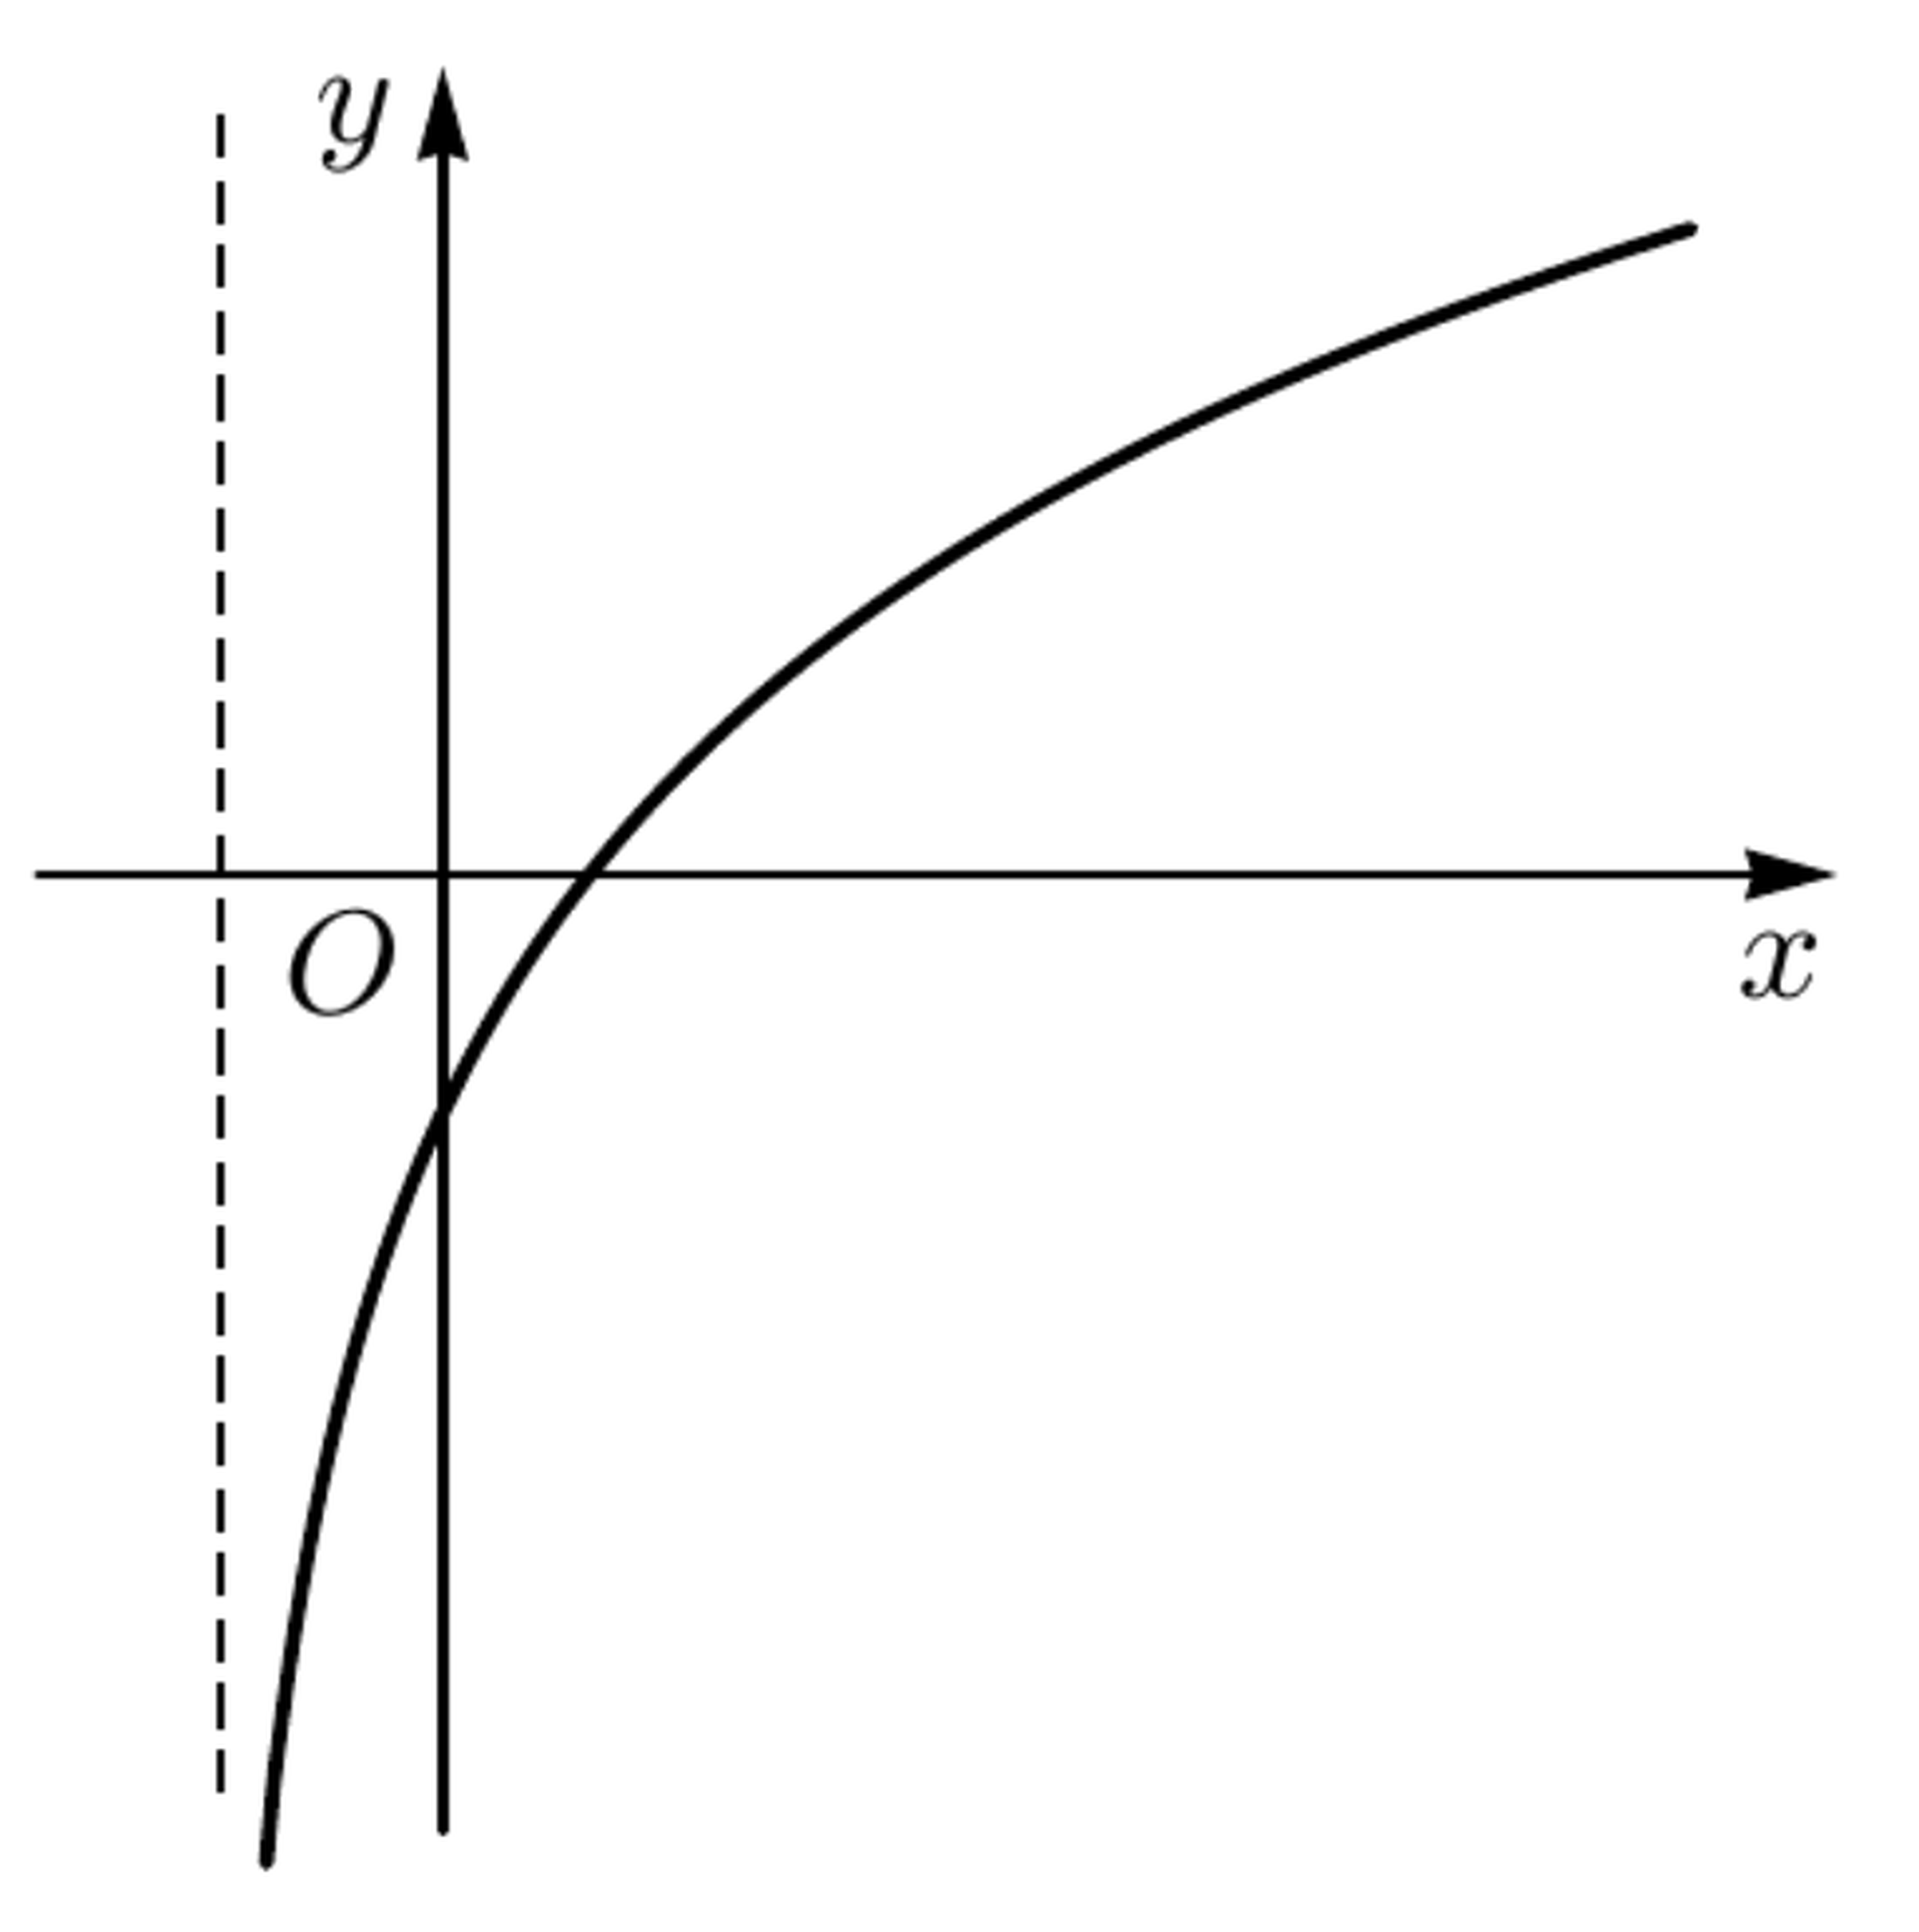
\includegraphics[width=0.42\textwidth]{figures/gao158_q15.png}
\end{center}

\keepwithprev
A. $a>1, b>1$\qquad\qquad B. $a>1, 0<b<1$

C. $0<a<1, b>1$\qquad\qquad D. $0<a<1, 0<b<1$

\ifanswer
\solbegin
\step{图像严格增，得 $a>1$.}
\step{图像与 $y$ 轴交于 $x$ 轴下方，得 $b>0$ 且 $\log_a b<0$，即 $0<b<1$，故选 $B$.}
\solend
\fi

% === Q16 === \lvert\log_2 x\rvert；解析 5 行，故选 C
\item 已知函数 $f(x)=\lvert\log_2 x\rvert$，若 $0<a<b$ 且 $f(a)=f(b)$，则 $a+2b$ 的取值范围是\mbox{（\quad）}

\keepwithprev
A. $(2\sqrt2,+\infty)$\qquad B. $[2\sqrt2,+\infty)$\qquad C. $(3,+\infty)$\qquad D. $[3,+\infty)$

\ifanswer
\solbegin
\step{由 $a<b$ 及 $\lvert\log_2 a\rvert=\lvert\log_2 b\rvert$，得 $\log_2 a=-\log_2 b$，即 $ab=1$，}
\step{且 $0<a<1<b$.}
\step{设 $t=a+2b=2b+\dfrac1b$，则 $t-3=\dfrac{(b-1)(2b-1)}{b}>0$.}
\step{反之，任取 $t>3$，令 $b=\dfrac{t+\sqrt{t^2-8}}{4}>1$、$a=\dfrac1b$，则满足题设且 $a+2b=t$.}
\step{因此取值范围为 $(3,+\infty)$，故选 $C$.}
\solend
\fi

\end{enumerate}

\bigsec{三、解答题}

\begin{enumerate}
\setcounter{enumi}{16}

% === Q17 === 集合、\overline{A}、\subseteq；解析 9 行
\item 已知全集 $U=\R$，集合 $A=\left\{x\mid\dfrac{x-3}{x+1}\leqslant0\right\}$，$B=\{x\mid x^2-2mx+m^2-9<0\}$（$m$ 为实数）.

(1) 当 $m=4$ 时，求 $A\cap B$ 和 $\overline{A}\cup B$；

(2) 若“$x\in A$”是“$x\in B$”的充分条件，求实数 $m$ 的取值范围.

\ifanswer
\solbegin
\step{(1) $\dfrac{x-3}{x+1}\leqslant0\Leftrightarrow-1<x\leqslant3$，所以 $A=(-1,3]$.}
\step{当 $m=4$ 时，$B=\{x\mid(x-4)^2<9\}=(1,7)$，}
\step{于是 $A\cap B=(1,3]$，$\overline{A}\cup B=(-\infty,-1]\cup(1,+\infty)$；}
\step{(2) $x^2-2mx+m^2-9<0\Leftrightarrow(x-m)^2<9$，所以 $B=(m-3,m+3)$.}
\step{题设充分条件等价于 $A\subseteq B$.}
\step{由于 $A=(-1,3]$，左端须满足 $m-3\leqslant-1$.}
\step{又 $3\in A$，须有 $3<m+3$.}
\step{这两个条件也保证 $(-1,3]\subseteq(m-3,m+3)$，}
\step{因此 $A\subseteq B\Leftrightarrow\begin{cases}m-3\leqslant-1\\m+3>3\end{cases}\Leftrightarrow0<m\leqslant2$.}
\solend
\fi

% === Q18 === 蓄水池造价（含 (3) 场地限制）；单位 \mathrm{m}；解析 13 行
\item 某工厂拟建一个容积为 $400\mathrm{m}^3$ 的无盖长方体蓄水池，池深 $4\mathrm{m}$，池底为矩形，其一边长
为 $x\mathrm{m}$. 池壁每平方米造价 100 元，池底每平方米造价 150 元. 设水池的总造价为 $C$
元.

(1) 把 $C$ 表示成 $x$ 的函数，并写出它的定义域；

(2) 当 $x$ 为何值时，总造价最低？最低造价是多少？

(3) 受场地限制，池底一边长 $x$ 不超过 $8\mathrm{m}$，此时总造价最低是多少？

\ifanswer
\solbegin
\step{(1) 设池底另一边长为 $y\mathrm{m}$，则 $4xy=400$，所以 $y=\dfrac{100}{x}$，$x>0$.}
\step{池底面积为 $100\mathrm{m}^2$，池壁总面积为 $8\left(x+\dfrac{100}{x}\right)\mathrm{m}^2$，}
\step{因此 $C(x)=100\times8\left(x+\dfrac{100}{x}\right)+150\times100=800x+\dfrac{80000}{x}+15000$，}
\step{定义域为 $(0,+\infty)$.}
\step{(2) 因为 $x>0$，所以 $C(x)=800\left(x+\dfrac{100}{x}\right)+15000$，}
\step{$\geqslant800\times2\sqrt{x\cdot\dfrac{100}{x}}+15000=31000$，}
\step{当且仅当 $x=\dfrac{100}{x}$，即 $x=10$ 时取等号.}
\step{答：当 $x=10$ 时，总造价最低，为 31000 元.}
\step{(3) 此时定义域为 $(0,8]$. 任取 $0<x_1<x_2\leqslant8$，}
\step{则 $C(x_2)-C(x_1)=800(x_2-x_1)\left(1-\dfrac{100}{x_1x_2}\right)<0$，}
\step{所以 $C(x)$ 在 $(0,8]$ 上严格递减，$x=8$ 时总造价最低，}
\step{且 $C(8)=800\times8+\dfrac{80000}{8}+15000=31400$.}
\step{答：受场地限制时，最低总造价为 31400 元.}
\solend
\fi

% === Q19 === 甲乙滤材 0.8^n／0.7^n；解析 17 行
\item 某环保公司研发了两种新型滤材甲和乙：污水每经过一层甲滤材，污染物含量减少
20\%；每经过一层乙滤材，污染物含量减少 30\%. 每层甲滤材成本 3 万元，每层乙滤材
成本 4 万元. 设原污水中污染物含量为 1，要求处理后污染物含量低于原来的 5\%.

(1) 若只使用一种滤材，污水经过 $n$ 层后污染物含量为 $y$，分别写出使用甲、乙两种滤材
时 $y$ 关于 $n$ 的函数关系式（$n$ 为正整数）；

(2) 若只使用一种滤材，分别求甲、乙至少各需要多少层，并比较哪种滤材的总成本更
低；

(3) 若两种滤材可以混合使用（先后顺序不影响效果），设使用甲滤材 $m$ 层、乙滤材 $n$
层（$m$、$n$ 为非负整数），求满足要求的最低总成本，并指出此时 $m$、$n$ 的值.

\ifanswer
\solbegin
\step{(1) 甲：$y=0.8^n$；乙：$y=0.7^n$，其中 $n$ 为正整数.}
\step{(2) 两种滤材均须满足 $y<0.05$，且污染物含量随层数增加而严格减少.}
\step{$0.8^{14}\approx0.04398<0.05<0.05498\approx0.8^{13}$，}
\step{$0.7^9=0.040353607<0.05<0.05764801=0.7^8$，}
\step{甲至少需要 14 层，成本为 $3\times14=42$ 万元；}
\step{乙至少需要 9 层，成本为 $4\times9=36$ 万元.}
\step{因此，只使用一种滤材时，使用乙滤材的总成本更低.}
\step{(3) 设总成本为 $C$ 万元，则 $C=3m+4n,0.8^m\cdot0.7^n<0.05,m,n\in\{0,1,2,\cdots\}$，}
\step{若 $m\geqslant3$，将其中 3 层甲替换为 2 层乙，}
\step{因为 $0.7^2=0.49<0.512=0.8^3,2\times4<3\times3$，}
\step{替换后污染物含量更低，成本减少 1 万元，因此最低成本方案必有 $m\leqslant2$.}
\step{当 $m=0$ 时，由第（2）小题得至少需要 9 层乙，最低成本为 36 万元.}
\step{当 $m=1$ 或 $m=2$ 时，$0.8\cdot0.7^7>0.8^2\cdot0.7^7=0.052706752>0.05$，}
\step{$0.8^2\cdot0.7^8<0.8\cdot0.7^8=0.046118408<0.05$，}
\step{因此两种情形均至少需要 8 层乙，}
\step{对应最低成本分别为 $3+4\times8=35$ 万元，$3\times2+4\times8=38$ 万元.}
\step{答：满足要求的最低总成本为 35 万元，此时使用甲滤材 1 层、乙滤材 8 层.}
\solend
\fi

% === Q20 === f(x)=\log_2(4^x+1)-x；\Delta；解析 17 行
\item 已知函数 $f(x)=\log_2(4^x+1)-x$.

(1) 证明 $f(x)=\log_2(2^x+2^{-x})$，并求 $f(x)$ 的最小值及取得最小值时 $x$ 的值；

(2) 解不等式 $f(x)>\log_2 5-1$；

(3) 证明：函数 $f(x)$ 在区间 $[0,+\infty)$ 上是严格增函数；并求使关于 $x$ 的方程 $f(x)=m$ 恰
有两个不同实数解的实数 $m$ 的取值范围.

\ifanswer
\solbegin
\step{(1) $f(x)=\log_2(4^x+1)-\log_2 2^x=\log_2\dfrac{4^x+1}{2^x}=\log_2(2^x+2^{-x})$，}
\step{因为 $2^x+2^{-x}\geqslant2\sqrt{2^x\cdot2^{-x}}=2$，所以 $f(x)\geqslant\log_2 2=1$，}
\step{等号当且仅当 $2^x=2^{-x}$，即 $x=0$ 时成立，故最小值为 1.}
\step{(2) 令 $t=2^x>0$，则 $f(x)>\log_2 5-1\Leftrightarrow t+\dfrac1t>\dfrac52\Leftrightarrow2t^2-5t+2>0$}
\step{$\Leftrightarrow(2t-1)(t-2)>0$，}
\step{结合 $t>0$，得 $0<t<\dfrac12$ 或 $t>2$，即 $x<-1$ 或 $x>1$，}
\step{解集为 $(-\infty,-1)\cup(1,+\infty)$.}
\step{(3) 任取 $0\leqslant x_1<x_2$，记 $a=2^{x_1}$，$b=2^{x_2}$，则 $1\leqslant a<b$，$ab>1$，}
\step{从而 $\left(b+\dfrac1b\right)-\left(a+\dfrac1a\right)=(b-a)\left(1-\dfrac{1}{ab}\right)>0$，}
\step{由对数函数的严格递增性，得 $f(x_1)<f(x_2)$，}
\step{所以 $f(x)$ 在 $[0,+\infty)$ 上是严格增函数.}
\step{当 $m<1$ 时，由（1）得方程无实数解；当 $m=1$ 时，只有实数解 $x=0$.}
\step{当 $m>1$ 时，令 $t=2^x>0$，则 $f(x)=m\Leftrightarrow t+\dfrac1t=2^m\Leftrightarrow t^2-2^m t+1=0$，}
\step{此时 $\Delta=2^{2m}-4>0$，两根之和为 $2^m>0$、之积为 $1>0$，}
\step{故有两个不同的正根.}
\step{每个正根 $t$ 唯一确定一个实数 $x=\log_2 t$，故原方程恰有两个不同实数解，}
\step{所求范围为 $m\in(1,+\infty)$.}
\solend
\fi

% === Q21 === f(x)=4^x-m\cdot2^{x+1}+3 值域与 h(m) 分段；解析 13 行
\item 已知函数 $f(x)=4^x-m\cdot2^{x+1}+3$（$m\in\R$），$x\in[0,2]$.

(1) 当 $m=1$ 时，求 $f(x)$ 的值域；

(2) 记 $f(x)$ 的最小值为 $h(m)$，求 $h(m)$ 的表达式；

(3) 若关于 $x$ 的方程 $f(x)=0$ 在区间 $[0,2]$ 上有解，求实数 $m$ 的取值范围.

\ifanswer
\solbegin
\step{令 $t=2^x$，则 $t\in[1,4]$，且 $f(x)=t^2-2mt+3=(t-m)^2+3-m^2$，}
\step{(1) 当 $m=1$ 时，$f(x)=(t-1)^2+2$.}
\step{由 $0\leqslant t-1\leqslant3$，得 $2\leqslant f(x)\leqslant11$，值域为 $[2,11]$.}
\step{(2) 二次函数 $y=(t-m)^2+3-m^2$ 的对称轴为直线 $t=m$.}
\step{当 $m\leqslant1$ 时，在 $t=1$ 处取最小值；}
\step{当 $1<m<4$ 时，在 $t=m$ 处取最小值；}
\step{当 $m\geqslant4$ 时，在 $t=4$ 处取最小值；}
\step{因此 $h(m)=\begin{cases}4-2m,&m\leqslant1\\3-m^2,&1<m<4\\19-8m,&m\geqslant4\end{cases}$；}
\step{(3) 方程 $f(x)=0$ 在 $[0,2]$ 上有解，}
\step{等价于存在 $t\in[1,4]$，使 $m=\dfrac{t^2+3}{2t}=\dfrac12\left(t+\dfrac3t\right)$，}
\step{由基本不等式，$m\geqslant\dfrac12\cdot2\sqrt{t\cdot\dfrac3t}=\sqrt3$，当且仅当 $t=\sqrt3$ 时取等号；}
\step{又 $\dfrac{19}{8}-m=\dfrac{(4-t)(4t-3)}{8t}\geqslant0$，当且仅当 $t=4$ 时取等号；}
\step{因此必有 $\sqrt3\leqslant m\leqslant\dfrac{19}{8}$.}
\solend
\fi

\end{enumerate}

\end{document}
